% Options for packages loaded elsewhere
\PassOptionsToPackage{unicode}{hyperref}
\PassOptionsToPackage{hyphens}{url}
%
\documentclass[
]{article}
\usepackage{lmodern}
\usepackage{amssymb,amsmath}
\usepackage{ifxetex,ifluatex}
\ifnum 0\ifxetex 1\fi\ifluatex 1\fi=0 % if pdftex
  \usepackage[T1]{fontenc}
  \usepackage[utf8]{inputenc}
  \usepackage{textcomp} % provide euro and other symbols
\else % if luatex or xetex
  \usepackage{unicode-math}
  \defaultfontfeatures{Scale=MatchLowercase}
  \defaultfontfeatures[\rmfamily]{Ligatures=TeX,Scale=1}
\fi
% Use upquote if available, for straight quotes in verbatim environments
\IfFileExists{upquote.sty}{\usepackage{upquote}}{}
\IfFileExists{microtype.sty}{% use microtype if available
  \usepackage[]{microtype}
  \UseMicrotypeSet[protrusion]{basicmath} % disable protrusion for tt fonts
}{}
\makeatletter
\@ifundefined{KOMAClassName}{% if non-KOMA class
  \IfFileExists{parskip.sty}{%
    \usepackage{parskip}
  }{% else
    \setlength{\parindent}{0pt}
    \setlength{\parskip}{6pt plus 2pt minus 1pt}}
}{% if KOMA class
  \KOMAoptions{parskip=half}}
\makeatother
\usepackage{xcolor}
\IfFileExists{xurl.sty}{\usepackage{xurl}}{} % add URL line breaks if available
\IfFileExists{bookmark.sty}{\usepackage{bookmark}}{\usepackage{hyperref}}
\hypersetup{
  pdftitle={Histopathology Research Template},
  hidelinks,
  pdfcreator={LaTeX via pandoc}}
\urlstyle{same} % disable monospaced font for URLs
\usepackage[margin=1in]{geometry}
\usepackage{color}
\usepackage{fancyvrb}
\newcommand{\VerbBar}{|}
\newcommand{\VERB}{\Verb[commandchars=\\\{\}]}
\DefineVerbatimEnvironment{Highlighting}{Verbatim}{commandchars=\\\{\}}
% Add ',fontsize=\small' for more characters per line
\usepackage{framed}
\definecolor{shadecolor}{RGB}{255,255,255}
\newenvironment{Shaded}{\begin{snugshade}}{\end{snugshade}}
\newcommand{\AlertTok}[1]{\textcolor[rgb]{0.75,0.01,0.01}{\textbf{\colorbox[rgb]{0.97,0.90,0.90}{#1}}}}
\newcommand{\AnnotationTok}[1]{\textcolor[rgb]{0.79,0.38,0.79}{#1}}
\newcommand{\AttributeTok}[1]{\textcolor[rgb]{0.00,0.34,0.68}{#1}}
\newcommand{\BaseNTok}[1]{\textcolor[rgb]{0.69,0.50,0.00}{#1}}
\newcommand{\BuiltInTok}[1]{\textcolor[rgb]{0.39,0.29,0.61}{\textbf{#1}}}
\newcommand{\CharTok}[1]{\textcolor[rgb]{0.57,0.30,0.62}{#1}}
\newcommand{\CommentTok}[1]{\textcolor[rgb]{0.54,0.53,0.53}{#1}}
\newcommand{\CommentVarTok}[1]{\textcolor[rgb]{0.00,0.58,1.00}{#1}}
\newcommand{\ConstantTok}[1]{\textcolor[rgb]{0.67,0.33,0.00}{#1}}
\newcommand{\ControlFlowTok}[1]{\textcolor[rgb]{0.12,0.11,0.11}{\textbf{#1}}}
\newcommand{\DataTypeTok}[1]{\textcolor[rgb]{0.00,0.34,0.68}{#1}}
\newcommand{\DecValTok}[1]{\textcolor[rgb]{0.69,0.50,0.00}{#1}}
\newcommand{\DocumentationTok}[1]{\textcolor[rgb]{0.38,0.47,0.50}{#1}}
\newcommand{\ErrorTok}[1]{\textcolor[rgb]{0.75,0.01,0.01}{\underline{#1}}}
\newcommand{\ExtensionTok}[1]{\textcolor[rgb]{0.00,0.58,1.00}{\textbf{#1}}}
\newcommand{\FloatTok}[1]{\textcolor[rgb]{0.69,0.50,0.00}{#1}}
\newcommand{\FunctionTok}[1]{\textcolor[rgb]{0.39,0.29,0.61}{#1}}
\newcommand{\ImportTok}[1]{\textcolor[rgb]{1.00,0.33,0.00}{#1}}
\newcommand{\InformationTok}[1]{\textcolor[rgb]{0.69,0.50,0.00}{#1}}
\newcommand{\KeywordTok}[1]{\textcolor[rgb]{0.12,0.11,0.11}{\textbf{#1}}}
\newcommand{\NormalTok}[1]{\textcolor[rgb]{0.12,0.11,0.11}{#1}}
\newcommand{\OperatorTok}[1]{\textcolor[rgb]{0.12,0.11,0.11}{#1}}
\newcommand{\OtherTok}[1]{\textcolor[rgb]{0.00,0.43,0.16}{#1}}
\newcommand{\PreprocessorTok}[1]{\textcolor[rgb]{0.00,0.43,0.16}{#1}}
\newcommand{\RegionMarkerTok}[1]{\textcolor[rgb]{0.00,0.34,0.68}{\colorbox[rgb]{0.88,0.91,0.97}{#1}}}
\newcommand{\SpecialCharTok}[1]{\textcolor[rgb]{0.24,0.68,0.91}{#1}}
\newcommand{\SpecialStringTok}[1]{\textcolor[rgb]{1.00,0.33,0.00}{#1}}
\newcommand{\StringTok}[1]{\textcolor[rgb]{0.75,0.01,0.01}{#1}}
\newcommand{\VariableTok}[1]{\textcolor[rgb]{0.00,0.34,0.68}{#1}}
\newcommand{\VerbatimStringTok}[1]{\textcolor[rgb]{0.75,0.01,0.01}{#1}}
\newcommand{\WarningTok}[1]{\textcolor[rgb]{0.75,0.01,0.01}{#1}}
\usepackage{longtable,booktabs}
% Correct order of tables after \paragraph or \subparagraph
\usepackage{etoolbox}
\makeatletter
\patchcmd\longtable{\par}{\if@noskipsec\mbox{}\fi\par}{}{}
\makeatother
% Allow footnotes in longtable head/foot
\IfFileExists{footnotehyper.sty}{\usepackage{footnotehyper}}{\usepackage{footnote}}
\makesavenoteenv{longtable}
\usepackage{graphicx,grffile}
\makeatletter
\def\maxwidth{\ifdim\Gin@nat@width>\linewidth\linewidth\else\Gin@nat@width\fi}
\def\maxheight{\ifdim\Gin@nat@height>\textheight\textheight\else\Gin@nat@height\fi}
\makeatother
% Scale images if necessary, so that they will not overflow the page
% margins by default, and it is still possible to overwrite the defaults
% using explicit options in \includegraphics[width, height, ...]{}
\setkeys{Gin}{width=\maxwidth,height=\maxheight,keepaspectratio}
% Set default figure placement to htbp
\makeatletter
\def\fps@figure{htbp}
\makeatother
\setlength{\emergencystretch}{3em} % prevent overfull lines
\providecommand{\tightlist}{%
  \setlength{\itemsep}{0pt}\setlength{\parskip}{0pt}}
\setcounter{secnumdepth}{5}
\usepackage{xcolor}
\definecolor{backgroundecho}{HTML}{cccccc}
\definecolor{textecho}{HTML}{333333}

\let\oldverbatim=\verbatim
\let\oldendverbatim=\endverbatim

\makeatletter
\renewenvironment{verbatim}{
    \def\FrameCommand{
        \hskip-\fboxsep
        \color{textecho}
        \colorbox{backgroundecho}
        }
    \MakeFramed{\@setminipage}
    \oldverbatim
}
{
    \oldendverbatim
    \vskip-2em\@minipagefalse % The size required for this negative space is probably in some variable
    \endMakeFramed
}
\makeatother
\usepackage{pdflscape}
\newcommand{\blandscape}{\begin{landscape}}
\newcommand{\elandscape}{\end{landscape}}
\usepackage{xcolor}
\usepackage{afterpage}
\renewcommand{\linethickness}{0.05em}
\usepackage{booktabs}
\usepackage{sectsty} \allsectionsfont{\nohang\centering \emph}
\usepackage{float}
\usepackage{svg}

\title{Histopathology Research Template}
\author{true}
\date{2020-02-26}

\begin{document}
\maketitle

{
\setcounter{tocdepth}{5}
\tableofcontents
}
\begin{center}\rule{0.5\linewidth}{0.5pt}\end{center}

\([![DOI](https://zenodo.org/badge/DOI/10.5281/zenodo.3635430.svg)](https://doi.org/10.5281/zenodo.3635430)\)

\url{https://doi.org/10.5281/zenodo.3635430}

\url{https://osf.io/3tjfk/}

\href{https://sbalci.github.io/histopathology-template/}{Histopathology
Research Template 🔬}

\begin{center}\rule{0.5\linewidth}{0.5pt}\end{center}

\hypertarget{introduction}{%
\section{Introduction}\label{introduction}}

\begin{itemize}
\tightlist
\item
  \textbf{State the marker of interest, the study objectives, and
  hypotheses (Knijn, Simmer, and Nagtegaal 2015)}.\footnote{From Table
    1: Proposed items for reporting histopathology studies.
    Recommendations for reporting histopathology studies: a proposal
    Virchows Arch (2015) 466:611--615 DOI 10.1007/s00428-015-1762-3
    \url{https://www.ncbi.nlm.nih.gov/pmc/articles/PMC4460276/}}
\end{itemize}

\hypertarget{materials-methods}{%
\section{Materials \& Methods}\label{materials-methods}}

\textbf{Describe Materials and Methods as highlighted in (Knijn, Simmer,
and Nagtegaal 2015)}.\footnote{From Table 1: Proposed items for
  reporting histopathology studies. Recommendations for reporting
  histopathology studies: a proposal Virchows Arch (2015) 466:611--615
  DOI 10.1007/s00428-015-1762-3
  \url{https://www.ncbi.nlm.nih.gov/pmc/articles/PMC4460276/}}

\begin{itemize}
\item
  Describe patient characteristics, and inclusion and exclusion criteria
\item
  Describe treatment details
\item
  Describe the type of material used
\item
  Specify how expression of the biomarker was assessed
\item
  Describe the number of independent (blinded) scorers and how they
  scored
\item
  State the method of case selection, study design, origin of the cases,
  and time frame
\item
  Describe the end of the follow-up period and median follow-up time
\item
  Define all clinical endpoints examined
\item
  Specify all applied statistical methods
\item
  Describe how interactions with other clinical/pathological factors
  were analyzed
\end{itemize}

\begin{center}\rule{0.5\linewidth}{0.5pt}\end{center}

\hypertarget{header-codes}{%
\subsection{Header Codes}\label{header-codes}}

\textbf{Codes for general settings.}\footnote{See
  \href{https://github.com/sbalci/histopathology-template/blob/master/childRmd/_01header.Rmd}{\texttt{childRmd/\_01header.Rmd}}
  file for other general settings}

\textbf{Setup global chunk settings}\footnote{Change
  \texttt{echo\ =\ FALSE} to hide codes after knitting and Change
  \texttt{cache\ =\ TRUE} to knit quickly. Change \texttt{error=TRUE} to
  continue rendering while errors are present.}

\begin{Shaded}
\begin{Highlighting}[]
\NormalTok{knitr}\OperatorTok{::}\NormalTok{opts_chunk}\OperatorTok{$}\KeywordTok{set}\NormalTok{(}
    \DataTypeTok{eval =} \OtherTok{TRUE}\NormalTok{,}
    \DataTypeTok{echo =} \OtherTok{TRUE}\NormalTok{,}
    \DataTypeTok{fig.path =}\NormalTok{ here}\OperatorTok{::}\KeywordTok{here}\NormalTok{(}\StringTok{"figs/"}\NormalTok{),}
    \DataTypeTok{message =} \OtherTok{FALSE}\NormalTok{,}
    \DataTypeTok{warning =} \OtherTok{FALSE}\NormalTok{,}
    \DataTypeTok{error =} \OtherTok{TRUE}\NormalTok{,}
    \DataTypeTok{cache =} \OtherTok{TRUE}\NormalTok{,}
    \DataTypeTok{comment =} \OtherTok{NA}\NormalTok{,}
    \DataTypeTok{tidy =} \OtherTok{TRUE}\NormalTok{,}
    \DataTypeTok{fig.width =} \DecValTok{6}\NormalTok{,}
    \DataTypeTok{fig.height =} \DecValTok{4}
\NormalTok{)}
\end{Highlighting}
\end{Shaded}

\begin{Shaded}
\begin{Highlighting}[]
\KeywordTok{library}\NormalTok{(knitr)}
\NormalTok{hook_output =}\StringTok{ }\NormalTok{knit_hooks}\OperatorTok{$}\KeywordTok{get}\NormalTok{(}\StringTok{"output"}\NormalTok{)}
\NormalTok{knit_hooks}\OperatorTok{$}\KeywordTok{set}\NormalTok{(}\DataTypeTok{output =} \ControlFlowTok{function}\NormalTok{(x, options) \{}
    \CommentTok{# this hook is used only when the linewidth option is not NULL}
    \ControlFlowTok{if}\NormalTok{ (}\OperatorTok{!}\KeywordTok{is.null}\NormalTok{(n <-}\StringTok{ }\NormalTok{options}\OperatorTok{$}\NormalTok{linewidth)) \{}
\NormalTok{        x =}\StringTok{ }\NormalTok{knitr}\OperatorTok{:::}\KeywordTok{split_lines}\NormalTok{(x)}
        \CommentTok{# any lines wider than n should be wrapped}
        \ControlFlowTok{if}\NormalTok{ (}\KeywordTok{any}\NormalTok{(}\KeywordTok{nchar}\NormalTok{(x) }\OperatorTok{>}\StringTok{ }\NormalTok{n)) }
\NormalTok{            x =}\StringTok{ }\KeywordTok{strwrap}\NormalTok{(x, }\DataTypeTok{width =}\NormalTok{ n)}
\NormalTok{        x =}\StringTok{ }\KeywordTok{paste}\NormalTok{(x, }\DataTypeTok{collapse =} \StringTok{"}\CharTok{\textbackslash{}n}\StringTok{"}\NormalTok{)}
\NormalTok{    \}}
    \KeywordTok{hook_output}\NormalTok{(x, options)}
\NormalTok{\})}
\end{Highlighting}
\end{Shaded}

\begin{Shaded}
\begin{Highlighting}[]
\NormalTok{# linewidth css}
\NormalTok{  pre}\InformationTok{:not(}\ExtensionTok{[class]}\InformationTok{)}\NormalTok{ \{}
    \KeywordTok{color}\NormalTok{: }\ConstantTok{#333333}\OperatorTok{;}
    \KeywordTok{background-color}\NormalTok{: }\ConstantTok{#cccccc}\OperatorTok{;}
\NormalTok{  \}}
\end{Highlighting}
\end{Shaded}

\begin{Shaded}
\begin{Highlighting}[]
\CommentTok{# linewidth css}
\end{Highlighting}
\end{Shaded}

\textbf{Load Library}

see
\href{https://github.com/sbalci/histopathology-template/blob/master/R/loadLibrary.R}{\texttt{R/loadLibrary.R}}
for the libraries loaded.

\begin{Shaded}
\begin{Highlighting}[]
\KeywordTok{source}\NormalTok{(}\DataTypeTok{file =}\NormalTok{ here}\OperatorTok{::}\KeywordTok{here}\NormalTok{(}\StringTok{"R"}\NormalTok{, }\StringTok{"loadLibrary.R"}\NormalTok{))}
\end{Highlighting}
\end{Shaded}

\begin{center}\rule{0.5\linewidth}{0.5pt}\end{center}

\hypertarget{generate-fake-data}{%
\subsection{Generate Fake Data}\label{generate-fake-data}}

\textbf{Codes for generating fake data}.\footnote{See
  \href{https://github.com/sbalci/histopathology-template/blob/master/childRmd/_02fakeData.Rmd}{\texttt{childRmd/\_02fakeData.Rmd}}
  file for other codes}

\textbf{Generate Fake Data}

This code generates a fake histopathological data. Some sources for fake
data generation here\footnote{Synthea The validity of synthetic clinical
  data: a validation study of a leading synthetic data generator
  (Synthea) using clinical quality measures. BMC Med Inform Decis Mak
  19, 44 (2019) \url{doi:10.1186/s12911-019-0793-0}} , here\footnote{\url{https://bmcmedinformdecismak.biomedcentral.com/articles/10.1186/s12911-019-0793-0}}
, here\footnote{\href{https://synthetichealth.github.io/synthea/}{Synthetic
  Patient Generation}} , here\footnote{\href{https://github.com/synthetichealth/synthea/wiki/Basic-Setup-and-Running}{Basic
  Setup and Running}} , here\footnote{\href{http://www.mli.gmu.edu/index.php/research/ipdg/}{intelligent
  patient data generator (iPDG)}} , here\footnote{\url{https://medium.com/free-code-camp/how-our-test-data-generator-makes-fake-data-look-real-ace01c5bde4a}}
, here\footnote{\url{https://forums.librehealth.io/t/demo-data-generation/203}}
, here\footnote{\url{https://mihin.org/services/patient-generator/}} ,
and here\footnote{lung, cancer, breast datası ile birleştir} .

\textbf{Use
\href{https://github.com/sbalci/histopathology-template/blob/master/R/gc_fake_data.R}{this
code} to generate fake clinicopathologic data}

\begin{Shaded}
\begin{Highlighting}[]
\KeywordTok{source}\NormalTok{(}\DataTypeTok{file =}\NormalTok{ here}\OperatorTok{::}\KeywordTok{here}\NormalTok{(}\StringTok{"R"}\NormalTok{, }\StringTok{"gc_fake_data.R"}\NormalTok{))}
\end{Highlighting}
\end{Shaded}

\begin{Shaded}
\begin{Highlighting}[]
\NormalTok{wakefield}\OperatorTok{::}\KeywordTok{table_heat}\NormalTok{(}\DataTypeTok{x =}\NormalTok{ fakedata, }\DataTypeTok{palette =} \StringTok{"Set1"}\NormalTok{, }\DataTypeTok{flip =} \OtherTok{TRUE}\NormalTok{, }\DataTypeTok{print =} \OtherTok{TRUE}\NormalTok{)}
\end{Highlighting}
\end{Shaded}

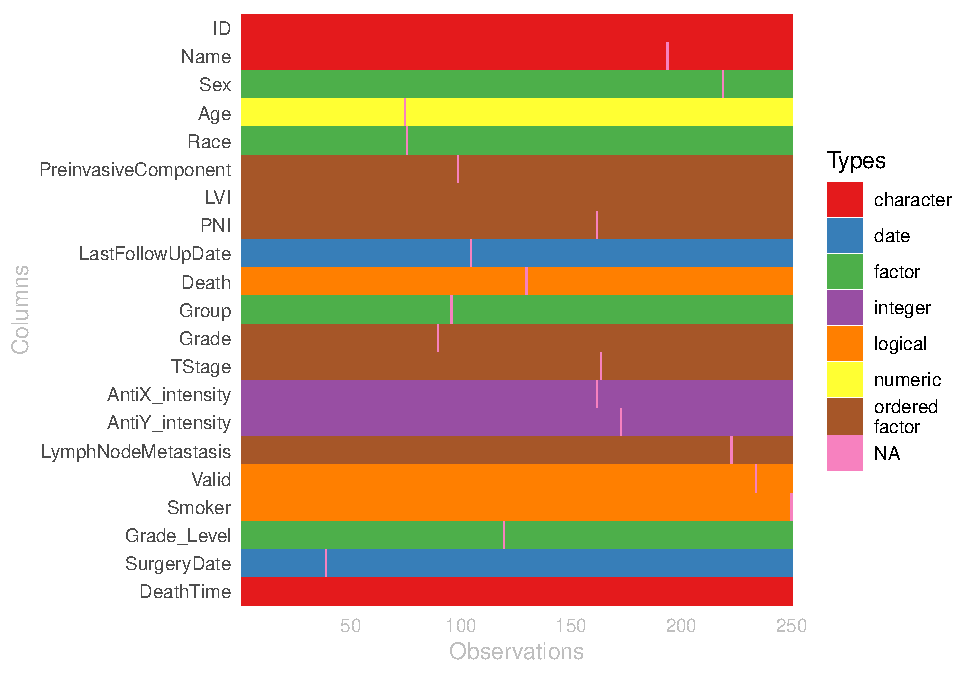
\includegraphics{/Users/serdarbalciold/histopathRprojects/histopathology-template/figs/plot fake data-1.pdf}

\begin{center}\rule{0.5\linewidth}{0.5pt}\end{center}

\hypertarget{import-data}{%
\subsection{Import Data}\label{import-data}}

\textbf{Codes for importing data.}\footnote{See
  \href{https://github.com/sbalci/histopathology-template/blob/master/childRmd/_03importData.Rmd}{\texttt{childRmd/\_03importData.Rmd}}
  file for other codes}

\textbf{Read the data}

\begin{Shaded}
\begin{Highlighting}[]
\KeywordTok{library}\NormalTok{(readxl)}
\NormalTok{mydata <-}\StringTok{ }\NormalTok{readxl}\OperatorTok{::}\KeywordTok{read_excel}\NormalTok{(here}\OperatorTok{::}\KeywordTok{here}\NormalTok{(}\StringTok{"data"}\NormalTok{, }\StringTok{"mydata.xlsx"}\NormalTok{))}
\CommentTok{# View(mydata) # Use to view data after importing}
\end{Highlighting}
\end{Shaded}

Add code for import multiple data purrr reduce

\begin{center}\rule{0.5\linewidth}{0.5pt}\end{center}

\hypertarget{study-population}{%
\subsection{Study Population}\label{study-population}}

\hypertarget{report-general-features}{%
\subsubsection{Report General Features}\label{report-general-features}}

\textbf{Codes for reporting general features.}\footnote{See
  \href{https://github.com/sbalci/histopathology-template/blob/master/childRmd/_04briefSummary.Rmd}{\texttt{childRmd/\_04briefSummary.Rmd}}
  file for other codes}

\textbf{Dataframe Report}

\begin{Shaded}
\begin{Highlighting}[]
\CommentTok{# Dataframe report}
\NormalTok{mydata }\OperatorTok\StringTok{ }\NormalTok{dplyr}\OperatorTok{::}\KeywordTok{select}\NormalTok{(}\OperatorTok{-}\KeywordTok{contains}\NormalTok{(}\StringTok{"Date"}\NormalTok{)) }\OperatorTok\StringTok{ }\NormalTok{report}\OperatorTok{::}\KeywordTok{report}\NormalTok{(.)}
\end{Highlighting}
\end{Shaded}

\begin{verbatim}
The data contains 250 observations of the following variables:
  - ID: 250 entries: 001, n = 1; 002, n = 1; 003, n = 1 and 247 others (0 missing)
  - Name: 249 entries: Aadan, n = 1; Aadhyan, n = 1; Abduljaleel, n = 1 and 246 others (1 missing)
  - Sex: 2 entries: Male, n = 134; Female, n = 115 (1 missing)
  - Age: Mean = 48.99, SD = 14.44, Median = , MAD = 19.27, range: [25, 73], Skewness = 0.03, Kurtosis = -1.28, 1 missing
  - Race: 7 entries: White, n = 167; Hispanic, n = 36; Black, n = 23 and 4 others (1 missing)
  - PreinvasiveComponent: 2 entries: Absent, n = 194; Present, n = 55 (1 missing)
  - LVI: 2 entries: Absent, n = 166; Present, n = 84 (0 missing)
  - PNI: 2 entries: Absent, n = 165; Present, n = 84 (1 missing)
  - Death: 2 levels: FALSE (n = 69, 27.60%); TRUE (n = 180, 72.00%) and missing (n = 1, 0.40%)
  - Group: 2 entries: Treatment, n = 129; Control, n = 120 (1 missing)
  - Grade: 3 entries: 3, n = 110; 2, n = 79; 1, n = 60 (1 missing)
  - TStage: 4 entries: 4, n = 117; 2, n = 58; 3, n = 53 and 1 other (1 missing)
  - AntiX_intensity: Mean = 2.42, SD = 0.64, Median = , MAD = 0.00, range: [1, 3], Skewness = -0.67, Kurtosis = -0.57, 1 missing
  - AntiY_intensity: Mean = 2.07, SD = 0.77, Median = , MAD = 1.48, range: [1, 3], Skewness = -0.12, Kurtosis = -1.29, 1 missing
  - LymphNodeMetastasis: 2 entries: Absent, n = 155; Present, n = 94 (1 missing)
  - Valid: 2 levels: FALSE (n = 135, 54.00%); TRUE (n = 114, 45.60%) and missing (n = 1, 0.40%)
  - Smoker: 2 levels: FALSE (n = 132, 52.80%); TRUE (n = 117, 46.80%) and missing (n = 1, 0.40%)
  - Grade_Level: 3 entries: high, n = 103; moderate, n = 78; low, n = 68 (1 missing)
  - DeathTime: 2 entries: Within1Year, n = 148; MoreThan1Year, n = 102 (0 missing)
\end{verbatim}

\begin{Shaded}
\begin{Highlighting}[]
\NormalTok{mydata }\OperatorTok\StringTok{ }\NormalTok{explore}\OperatorTok{::}\KeywordTok{describe_tbl}\NormalTok{()}
\end{Highlighting}
\end{Shaded}

\begin{verbatim}
250 observations with 21 variables
18 variables containing missings (NA)
0 variables with no variance
\end{verbatim}

\begin{center}\rule{0.5\linewidth}{0.5pt}\end{center}

\hypertarget{ethics-and-irb}{%
\subsection{Ethics and IRB}\label{ethics-and-irb}}

\hypertarget{always-respect-patient-privacy}{%
\subsubsection{Always Respect Patient
Privacy}\label{always-respect-patient-privacy}}

\textbf{Always Respect Patient Privacy}\\
- Health Information Privacy\footnote{\url{https://www.hhs.gov/hipaa/index.html}}~\\
- Kişisel Verilerin Korunması\footnote{\href{https://barandogan.av.tr/blog/ceza-hukuku/kisisel-verilerin-ele-gecirilmesi-yayilmasi-baskasina-verilmesi-sucu.html}{Kişisel
  verilerin kaydedilmesi ve kişisel verileri hukuka aykırı olarak verme
  veya ele geçirme Türk Ceza Kanunu'nun 135. ve 136. maddesi kapsamında
  bizim hukuk sistemimizde suç olarak tanımlanmıştır. Kişisel verilerin
  kaydedilmesi suçunun cezası 1 ila 3 yıl hapis cezasıdır. Suçun
  nitelikli hali ise, kamu görevlisi tarafından görevin verdiği yetkinin
  kötüye kullanılarak veya belirli bir meslek veya sanatın sağladığı
  kolaylıktan yararlanılarak işlenmesidir ki bu durumda suçun cezası 1.5
  ile 4.5 yıl hapis cezası olacaktır.}}

\noindent

\colorbox{yellow}{
\parbox{\dimexpr\linewidth-2\fboxsep}{

**Always Respect Patient Privacy**  
- Health Information Privacy^[https://www.hhs.gov/hipaa/index.html]  
- Kişisel Verilerin Korunması^[[Kişisel verilerin kaydedilmesi ve kişisel verileri hukuka aykırı olarak verme veya ele geçirme Türk Ceza Kanunu'nun 135. ve 136. maddesi kapsamında bizim hukuk sistemimizde suç olarak tanımlanmıştır. Kişisel verilerin kaydedilmesi suçunun cezası 1 ila 3 yıl hapis cezasıdır. Suçun nitelikli hali ise, kamu görevlisi tarafından görevin verdiği yetkinin kötüye kullanılarak veya belirli bir meslek veya sanatın sağladığı kolaylıktan yararlanılarak işlenmesidir ki bu durumda suçun cezası 1.5 ile 4.5 yıl hapis cezası olacaktır.](https://barandogan.av.tr/blog/ceza-hukuku/kisisel-verilerin-ele-gecirilmesi-yayilmasi-baskasina-verilmesi-sucu.html)]  

}
}

\begin{center}\rule{0.5\linewidth}{0.5pt}\end{center}

\hypertarget{define-variable-types}{%
\subsection{Define Variable Types}\label{define-variable-types}}

\textbf{Codes for defining variable types}.\footnote{See
  \href{https://github.com/sbalci/histopathology-template/blob/master/childRmd/_06variableTypes.Rmd}{\texttt{childRmd/\_06variableTypes.Rmd}}
  file for other codes}

\textbf{print column names as vector}

\begin{Shaded}
\begin{Highlighting}[]
\KeywordTok{dput}\NormalTok{(}\KeywordTok{names}\NormalTok{(mydata))}
\end{Highlighting}
\end{Shaded}

\begin{verbatim}
c("ID", "Name", "Sex", "Age", "Race", "PreinvasiveComponent", 
"LVI", "PNI", "LastFollowUpDate", "Death", "Group", "Grade", 
"TStage", "AntiX_intensity", "AntiY_intensity", "LymphNodeMetastasis", 
"Valid", "Smoker", "Grade_Level", "SurgeryDate", "DeathTime")
\end{verbatim}

\hypertarget{find-key-columns}{%
\subsubsection{Find Key Columns}\label{find-key-columns}}

\hypertarget{find-id-and-key-columns-to-exclude-from-analysis}{%
\paragraph{Find ID and key columns to exclude from
analysis}\label{find-id-and-key-columns-to-exclude-from-analysis}}

\begin{verbatim}
vctrs::vec_assert()

dplyr::all_equal()

arsenal::compare()

visdat::vis_compare()
\end{verbatim}

See the code as function in
\href{https://github.com/sbalci/histopathology-template/blob/master/R/find_key.R}{\texttt{R/find\_key.R}}.

\begin{Shaded}
\begin{Highlighting}[]
\NormalTok{keycolumns <-}\StringTok{ }\NormalTok{mydata }\OperatorTok\StringTok{ }\KeywordTok{sapply}\NormalTok{(., }\DataTypeTok{FUN =}\NormalTok{ dataMaid}\OperatorTok{::}\NormalTok{isKey) }\OperatorTok\StringTok{ }\NormalTok{tibble}\OperatorTok{::}\KeywordTok{as_tibble}\NormalTok{() }\OperatorTok\StringTok{ }
\StringTok{    }\NormalTok{dplyr}\OperatorTok{::}\KeywordTok{select}\NormalTok{(}\KeywordTok{which}\NormalTok{(.[}\DecValTok{1}\NormalTok{, ] }\OperatorTok{==}\StringTok{ }\OtherTok{TRUE}\NormalTok{)) }\OperatorTok\StringTok{ }\KeywordTok{names}\NormalTok{()}
\NormalTok{keycolumns}
\end{Highlighting}
\end{Shaded}

\begin{verbatim}
[1] "ID"   "Name"
\end{verbatim}

\hypertarget{variable-types}{%
\subsubsection{Variable Types}\label{variable-types}}

\textbf{Get variable types}

\begin{Shaded}
\begin{Highlighting}[]
\NormalTok{mydata }\OperatorTok\StringTok{ }\NormalTok{dplyr}\OperatorTok{::}\KeywordTok{select}\NormalTok{(}\OperatorTok{-}\NormalTok{keycolumns) }\OperatorTok\StringTok{ }\NormalTok{inspectdf}\OperatorTok{::}\KeywordTok{inspect_types}\NormalTok{()}
\end{Highlighting}
\end{Shaded}

\begin{verbatim}
# A tibble: 4 x 4
  type             cnt  pcnt col_name  
  <chr>          <int> <dbl> <list>    
1 character         11  57.9 <chr [11]>
2 logical            3  15.8 <chr [3]> 
3 numeric            3  15.8 <chr [3]> 
4 POSIXct POSIXt     2  10.5 <chr [2]> 
\end{verbatim}

\begin{Shaded}
\begin{Highlighting}[]
\NormalTok{mydata }\OperatorTok\StringTok{ }\NormalTok{dplyr}\OperatorTok{::}\KeywordTok{select}\NormalTok{(}\OperatorTok{-}\NormalTok{keycolumns, }\OperatorTok{-}\KeywordTok{contains}\NormalTok{(}\StringTok{"Date"}\NormalTok{)) }\OperatorTok\StringTok{ }\NormalTok{describer}\OperatorTok{::}\KeywordTok{describe}\NormalTok{() }\OperatorTok\StringTok{ }
\StringTok{    }\NormalTok{knitr}\OperatorTok{::}\KeywordTok{kable}\NormalTok{(}\DataTypeTok{format =} \StringTok{"markdown"}\NormalTok{)}
\end{Highlighting}
\end{Shaded}

\begin{longtable}[]{@{}lllrrrlrrrl@{}}
\toprule
\begin{minipage}[b]{0.10\columnwidth}\raggedright
.column\_name\strut
\end{minipage} & \begin{minipage}[b]{0.07\columnwidth}\raggedright
.column\_class\strut
\end{minipage} & \begin{minipage}[b]{0.06\columnwidth}\raggedright
.column\_type\strut
\end{minipage} & \begin{minipage}[b]{0.08\columnwidth}\raggedleft
.count\_elements\strut
\end{minipage} & \begin{minipage}[b]{0.06\columnwidth}\raggedleft
.mean\_value\strut
\end{minipage} & \begin{minipage}[b]{0.05\columnwidth}\raggedleft
.sd\_value\strut
\end{minipage} & \begin{minipage}[b]{0.07\columnwidth}\raggedright
.q0\_value\strut
\end{minipage} & \begin{minipage}[b]{0.05\columnwidth}\raggedleft
.q25\_value\strut
\end{minipage} & \begin{minipage}[b]{0.05\columnwidth}\raggedleft
.q50\_value\strut
\end{minipage} & \begin{minipage}[b]{0.05\columnwidth}\raggedleft
.q75\_value\strut
\end{minipage} & \begin{minipage}[b]{0.06\columnwidth}\raggedright
.q100\_value\strut
\end{minipage}\tabularnewline
\midrule
\endhead
\begin{minipage}[t]{0.10\columnwidth}\raggedright
Sex\strut
\end{minipage} & \begin{minipage}[t]{0.07\columnwidth}\raggedright
character\strut
\end{minipage} & \begin{minipage}[t]{0.06\columnwidth}\raggedright
character\strut
\end{minipage} & \begin{minipage}[t]{0.08\columnwidth}\raggedleft
250\strut
\end{minipage} & \begin{minipage}[t]{0.06\columnwidth}\raggedleft
NA\strut
\end{minipage} & \begin{minipage}[t]{0.05\columnwidth}\raggedleft
NA\strut
\end{minipage} & \begin{minipage}[t]{0.07\columnwidth}\raggedright
Female\strut
\end{minipage} & \begin{minipage}[t]{0.05\columnwidth}\raggedleft
NA\strut
\end{minipage} & \begin{minipage}[t]{0.05\columnwidth}\raggedleft
NA\strut
\end{minipage} & \begin{minipage}[t]{0.05\columnwidth}\raggedleft
NA\strut
\end{minipage} & \begin{minipage}[t]{0.06\columnwidth}\raggedright
Male\strut
\end{minipage}\tabularnewline
\begin{minipage}[t]{0.10\columnwidth}\raggedright
Age\strut
\end{minipage} & \begin{minipage}[t]{0.07\columnwidth}\raggedright
numeric\strut
\end{minipage} & \begin{minipage}[t]{0.06\columnwidth}\raggedright
double\strut
\end{minipage} & \begin{minipage}[t]{0.08\columnwidth}\raggedleft
250\strut
\end{minipage} & \begin{minipage}[t]{0.06\columnwidth}\raggedleft
48.991968\strut
\end{minipage} & \begin{minipage}[t]{0.05\columnwidth}\raggedleft
14.4417607\strut
\end{minipage} & \begin{minipage}[t]{0.07\columnwidth}\raggedright
25\strut
\end{minipage} & \begin{minipage}[t]{0.05\columnwidth}\raggedleft
36\strut
\end{minipage} & \begin{minipage}[t]{0.05\columnwidth}\raggedleft
50\strut
\end{minipage} & \begin{minipage}[t]{0.05\columnwidth}\raggedleft
62\strut
\end{minipage} & \begin{minipage}[t]{0.06\columnwidth}\raggedright
73\strut
\end{minipage}\tabularnewline
\begin{minipage}[t]{0.10\columnwidth}\raggedright
Race\strut
\end{minipage} & \begin{minipage}[t]{0.07\columnwidth}\raggedright
character\strut
\end{minipage} & \begin{minipage}[t]{0.06\columnwidth}\raggedright
character\strut
\end{minipage} & \begin{minipage}[t]{0.08\columnwidth}\raggedleft
250\strut
\end{minipage} & \begin{minipage}[t]{0.06\columnwidth}\raggedleft
NA\strut
\end{minipage} & \begin{minipage}[t]{0.05\columnwidth}\raggedleft
NA\strut
\end{minipage} & \begin{minipage}[t]{0.07\columnwidth}\raggedright
Asian\strut
\end{minipage} & \begin{minipage}[t]{0.05\columnwidth}\raggedleft
NA\strut
\end{minipage} & \begin{minipage}[t]{0.05\columnwidth}\raggedleft
NA\strut
\end{minipage} & \begin{minipage}[t]{0.05\columnwidth}\raggedleft
NA\strut
\end{minipage} & \begin{minipage}[t]{0.06\columnwidth}\raggedright
White\strut
\end{minipage}\tabularnewline
\begin{minipage}[t]{0.10\columnwidth}\raggedright
PreinvasiveComponent\strut
\end{minipage} & \begin{minipage}[t]{0.07\columnwidth}\raggedright
character\strut
\end{minipage} & \begin{minipage}[t]{0.06\columnwidth}\raggedright
character\strut
\end{minipage} & \begin{minipage}[t]{0.08\columnwidth}\raggedleft
250\strut
\end{minipage} & \begin{minipage}[t]{0.06\columnwidth}\raggedleft
NA\strut
\end{minipage} & \begin{minipage}[t]{0.05\columnwidth}\raggedleft
NA\strut
\end{minipage} & \begin{minipage}[t]{0.07\columnwidth}\raggedright
Absent\strut
\end{minipage} & \begin{minipage}[t]{0.05\columnwidth}\raggedleft
NA\strut
\end{minipage} & \begin{minipage}[t]{0.05\columnwidth}\raggedleft
NA\strut
\end{minipage} & \begin{minipage}[t]{0.05\columnwidth}\raggedleft
NA\strut
\end{minipage} & \begin{minipage}[t]{0.06\columnwidth}\raggedright
Present\strut
\end{minipage}\tabularnewline
\begin{minipage}[t]{0.10\columnwidth}\raggedright
LVI\strut
\end{minipage} & \begin{minipage}[t]{0.07\columnwidth}\raggedright
character\strut
\end{minipage} & \begin{minipage}[t]{0.06\columnwidth}\raggedright
character\strut
\end{minipage} & \begin{minipage}[t]{0.08\columnwidth}\raggedleft
250\strut
\end{minipage} & \begin{minipage}[t]{0.06\columnwidth}\raggedleft
NA\strut
\end{minipage} & \begin{minipage}[t]{0.05\columnwidth}\raggedleft
NA\strut
\end{minipage} & \begin{minipage}[t]{0.07\columnwidth}\raggedright
Absent\strut
\end{minipage} & \begin{minipage}[t]{0.05\columnwidth}\raggedleft
NA\strut
\end{minipage} & \begin{minipage}[t]{0.05\columnwidth}\raggedleft
NA\strut
\end{minipage} & \begin{minipage}[t]{0.05\columnwidth}\raggedleft
NA\strut
\end{minipage} & \begin{minipage}[t]{0.06\columnwidth}\raggedright
Present\strut
\end{minipage}\tabularnewline
\begin{minipage}[t]{0.10\columnwidth}\raggedright
PNI\strut
\end{minipage} & \begin{minipage}[t]{0.07\columnwidth}\raggedright
character\strut
\end{minipage} & \begin{minipage}[t]{0.06\columnwidth}\raggedright
character\strut
\end{minipage} & \begin{minipage}[t]{0.08\columnwidth}\raggedleft
250\strut
\end{minipage} & \begin{minipage}[t]{0.06\columnwidth}\raggedleft
NA\strut
\end{minipage} & \begin{minipage}[t]{0.05\columnwidth}\raggedleft
NA\strut
\end{minipage} & \begin{minipage}[t]{0.07\columnwidth}\raggedright
Absent\strut
\end{minipage} & \begin{minipage}[t]{0.05\columnwidth}\raggedleft
NA\strut
\end{minipage} & \begin{minipage}[t]{0.05\columnwidth}\raggedleft
NA\strut
\end{minipage} & \begin{minipage}[t]{0.05\columnwidth}\raggedleft
NA\strut
\end{minipage} & \begin{minipage}[t]{0.06\columnwidth}\raggedright
Present\strut
\end{minipage}\tabularnewline
\begin{minipage}[t]{0.10\columnwidth}\raggedright
Death\strut
\end{minipage} & \begin{minipage}[t]{0.07\columnwidth}\raggedright
logical\strut
\end{minipage} & \begin{minipage}[t]{0.06\columnwidth}\raggedright
logical\strut
\end{minipage} & \begin{minipage}[t]{0.08\columnwidth}\raggedleft
250\strut
\end{minipage} & \begin{minipage}[t]{0.06\columnwidth}\raggedleft
NA\strut
\end{minipage} & \begin{minipage}[t]{0.05\columnwidth}\raggedleft
NA\strut
\end{minipage} & \begin{minipage}[t]{0.07\columnwidth}\raggedright
FALSE\strut
\end{minipage} & \begin{minipage}[t]{0.05\columnwidth}\raggedleft
NA\strut
\end{minipage} & \begin{minipage}[t]{0.05\columnwidth}\raggedleft
NA\strut
\end{minipage} & \begin{minipage}[t]{0.05\columnwidth}\raggedleft
NA\strut
\end{minipage} & \begin{minipage}[t]{0.06\columnwidth}\raggedright
TRUE\strut
\end{minipage}\tabularnewline
\begin{minipage}[t]{0.10\columnwidth}\raggedright
Group\strut
\end{minipage} & \begin{minipage}[t]{0.07\columnwidth}\raggedright
character\strut
\end{minipage} & \begin{minipage}[t]{0.06\columnwidth}\raggedright
character\strut
\end{minipage} & \begin{minipage}[t]{0.08\columnwidth}\raggedleft
250\strut
\end{minipage} & \begin{minipage}[t]{0.06\columnwidth}\raggedleft
NA\strut
\end{minipage} & \begin{minipage}[t]{0.05\columnwidth}\raggedleft
NA\strut
\end{minipage} & \begin{minipage}[t]{0.07\columnwidth}\raggedright
Control\strut
\end{minipage} & \begin{minipage}[t]{0.05\columnwidth}\raggedleft
NA\strut
\end{minipage} & \begin{minipage}[t]{0.05\columnwidth}\raggedleft
NA\strut
\end{minipage} & \begin{minipage}[t]{0.05\columnwidth}\raggedleft
NA\strut
\end{minipage} & \begin{minipage}[t]{0.06\columnwidth}\raggedright
Treatment\strut
\end{minipage}\tabularnewline
\begin{minipage}[t]{0.10\columnwidth}\raggedright
Grade\strut
\end{minipage} & \begin{minipage}[t]{0.07\columnwidth}\raggedright
character\strut
\end{minipage} & \begin{minipage}[t]{0.06\columnwidth}\raggedright
character\strut
\end{minipage} & \begin{minipage}[t]{0.08\columnwidth}\raggedleft
250\strut
\end{minipage} & \begin{minipage}[t]{0.06\columnwidth}\raggedleft
NA\strut
\end{minipage} & \begin{minipage}[t]{0.05\columnwidth}\raggedleft
NA\strut
\end{minipage} & \begin{minipage}[t]{0.07\columnwidth}\raggedright
1\strut
\end{minipage} & \begin{minipage}[t]{0.05\columnwidth}\raggedleft
NA\strut
\end{minipage} & \begin{minipage}[t]{0.05\columnwidth}\raggedleft
NA\strut
\end{minipage} & \begin{minipage}[t]{0.05\columnwidth}\raggedleft
NA\strut
\end{minipage} & \begin{minipage}[t]{0.06\columnwidth}\raggedright
3\strut
\end{minipage}\tabularnewline
\begin{minipage}[t]{0.10\columnwidth}\raggedright
TStage\strut
\end{minipage} & \begin{minipage}[t]{0.07\columnwidth}\raggedright
character\strut
\end{minipage} & \begin{minipage}[t]{0.06\columnwidth}\raggedright
character\strut
\end{minipage} & \begin{minipage}[t]{0.08\columnwidth}\raggedleft
250\strut
\end{minipage} & \begin{minipage}[t]{0.06\columnwidth}\raggedleft
NA\strut
\end{minipage} & \begin{minipage}[t]{0.05\columnwidth}\raggedleft
NA\strut
\end{minipage} & \begin{minipage}[t]{0.07\columnwidth}\raggedright
1\strut
\end{minipage} & \begin{minipage}[t]{0.05\columnwidth}\raggedleft
NA\strut
\end{minipage} & \begin{minipage}[t]{0.05\columnwidth}\raggedleft
NA\strut
\end{minipage} & \begin{minipage}[t]{0.05\columnwidth}\raggedleft
NA\strut
\end{minipage} & \begin{minipage}[t]{0.06\columnwidth}\raggedright
4\strut
\end{minipage}\tabularnewline
\begin{minipage}[t]{0.10\columnwidth}\raggedright
AntiX\_intensity\strut
\end{minipage} & \begin{minipage}[t]{0.07\columnwidth}\raggedright
numeric\strut
\end{minipage} & \begin{minipage}[t]{0.06\columnwidth}\raggedright
double\strut
\end{minipage} & \begin{minipage}[t]{0.08\columnwidth}\raggedleft
250\strut
\end{minipage} & \begin{minipage}[t]{0.06\columnwidth}\raggedleft
2.421687\strut
\end{minipage} & \begin{minipage}[t]{0.05\columnwidth}\raggedleft
0.6435878\strut
\end{minipage} & \begin{minipage}[t]{0.07\columnwidth}\raggedright
1\strut
\end{minipage} & \begin{minipage}[t]{0.05\columnwidth}\raggedleft
2\strut
\end{minipage} & \begin{minipage}[t]{0.05\columnwidth}\raggedleft
3\strut
\end{minipage} & \begin{minipage}[t]{0.05\columnwidth}\raggedleft
3\strut
\end{minipage} & \begin{minipage}[t]{0.06\columnwidth}\raggedright
3\strut
\end{minipage}\tabularnewline
\begin{minipage}[t]{0.10\columnwidth}\raggedright
AntiY\_intensity\strut
\end{minipage} & \begin{minipage}[t]{0.07\columnwidth}\raggedright
numeric\strut
\end{minipage} & \begin{minipage}[t]{0.06\columnwidth}\raggedright
double\strut
\end{minipage} & \begin{minipage}[t]{0.08\columnwidth}\raggedleft
250\strut
\end{minipage} & \begin{minipage}[t]{0.06\columnwidth}\raggedleft
2.068273\strut
\end{minipage} & \begin{minipage}[t]{0.05\columnwidth}\raggedleft
0.7668520\strut
\end{minipage} & \begin{minipage}[t]{0.07\columnwidth}\raggedright
1\strut
\end{minipage} & \begin{minipage}[t]{0.05\columnwidth}\raggedleft
1\strut
\end{minipage} & \begin{minipage}[t]{0.05\columnwidth}\raggedleft
2\strut
\end{minipage} & \begin{minipage}[t]{0.05\columnwidth}\raggedleft
3\strut
\end{minipage} & \begin{minipage}[t]{0.06\columnwidth}\raggedright
3\strut
\end{minipage}\tabularnewline
\begin{minipage}[t]{0.10\columnwidth}\raggedright
LymphNodeMetastasis\strut
\end{minipage} & \begin{minipage}[t]{0.07\columnwidth}\raggedright
character\strut
\end{minipage} & \begin{minipage}[t]{0.06\columnwidth}\raggedright
character\strut
\end{minipage} & \begin{minipage}[t]{0.08\columnwidth}\raggedleft
250\strut
\end{minipage} & \begin{minipage}[t]{0.06\columnwidth}\raggedleft
NA\strut
\end{minipage} & \begin{minipage}[t]{0.05\columnwidth}\raggedleft
NA\strut
\end{minipage} & \begin{minipage}[t]{0.07\columnwidth}\raggedright
Absent\strut
\end{minipage} & \begin{minipage}[t]{0.05\columnwidth}\raggedleft
NA\strut
\end{minipage} & \begin{minipage}[t]{0.05\columnwidth}\raggedleft
NA\strut
\end{minipage} & \begin{minipage}[t]{0.05\columnwidth}\raggedleft
NA\strut
\end{minipage} & \begin{minipage}[t]{0.06\columnwidth}\raggedright
Present\strut
\end{minipage}\tabularnewline
\begin{minipage}[t]{0.10\columnwidth}\raggedright
Valid\strut
\end{minipage} & \begin{minipage}[t]{0.07\columnwidth}\raggedright
logical\strut
\end{minipage} & \begin{minipage}[t]{0.06\columnwidth}\raggedright
logical\strut
\end{minipage} & \begin{minipage}[t]{0.08\columnwidth}\raggedleft
250\strut
\end{minipage} & \begin{minipage}[t]{0.06\columnwidth}\raggedleft
NA\strut
\end{minipage} & \begin{minipage}[t]{0.05\columnwidth}\raggedleft
NA\strut
\end{minipage} & \begin{minipage}[t]{0.07\columnwidth}\raggedright
FALSE\strut
\end{minipage} & \begin{minipage}[t]{0.05\columnwidth}\raggedleft
NA\strut
\end{minipage} & \begin{minipage}[t]{0.05\columnwidth}\raggedleft
NA\strut
\end{minipage} & \begin{minipage}[t]{0.05\columnwidth}\raggedleft
NA\strut
\end{minipage} & \begin{minipage}[t]{0.06\columnwidth}\raggedright
TRUE\strut
\end{minipage}\tabularnewline
\begin{minipage}[t]{0.10\columnwidth}\raggedright
Smoker\strut
\end{minipage} & \begin{minipage}[t]{0.07\columnwidth}\raggedright
logical\strut
\end{minipage} & \begin{minipage}[t]{0.06\columnwidth}\raggedright
logical\strut
\end{minipage} & \begin{minipage}[t]{0.08\columnwidth}\raggedleft
250\strut
\end{minipage} & \begin{minipage}[t]{0.06\columnwidth}\raggedleft
NA\strut
\end{minipage} & \begin{minipage}[t]{0.05\columnwidth}\raggedleft
NA\strut
\end{minipage} & \begin{minipage}[t]{0.07\columnwidth}\raggedright
FALSE\strut
\end{minipage} & \begin{minipage}[t]{0.05\columnwidth}\raggedleft
NA\strut
\end{minipage} & \begin{minipage}[t]{0.05\columnwidth}\raggedleft
NA\strut
\end{minipage} & \begin{minipage}[t]{0.05\columnwidth}\raggedleft
NA\strut
\end{minipage} & \begin{minipage}[t]{0.06\columnwidth}\raggedright
TRUE\strut
\end{minipage}\tabularnewline
\begin{minipage}[t]{0.10\columnwidth}\raggedright
Grade\_Level\strut
\end{minipage} & \begin{minipage}[t]{0.07\columnwidth}\raggedright
character\strut
\end{minipage} & \begin{minipage}[t]{0.06\columnwidth}\raggedright
character\strut
\end{minipage} & \begin{minipage}[t]{0.08\columnwidth}\raggedleft
250\strut
\end{minipage} & \begin{minipage}[t]{0.06\columnwidth}\raggedleft
NA\strut
\end{minipage} & \begin{minipage}[t]{0.05\columnwidth}\raggedleft
NA\strut
\end{minipage} & \begin{minipage}[t]{0.07\columnwidth}\raggedright
high\strut
\end{minipage} & \begin{minipage}[t]{0.05\columnwidth}\raggedleft
NA\strut
\end{minipage} & \begin{minipage}[t]{0.05\columnwidth}\raggedleft
NA\strut
\end{minipage} & \begin{minipage}[t]{0.05\columnwidth}\raggedleft
NA\strut
\end{minipage} & \begin{minipage}[t]{0.06\columnwidth}\raggedright
moderate\strut
\end{minipage}\tabularnewline
\begin{minipage}[t]{0.10\columnwidth}\raggedright
DeathTime\strut
\end{minipage} & \begin{minipage}[t]{0.07\columnwidth}\raggedright
character\strut
\end{minipage} & \begin{minipage}[t]{0.06\columnwidth}\raggedright
character\strut
\end{minipage} & \begin{minipage}[t]{0.08\columnwidth}\raggedleft
250\strut
\end{minipage} & \begin{minipage}[t]{0.06\columnwidth}\raggedleft
NA\strut
\end{minipage} & \begin{minipage}[t]{0.05\columnwidth}\raggedleft
NA\strut
\end{minipage} & \begin{minipage}[t]{0.07\columnwidth}\raggedright
MoreThan1Year\strut
\end{minipage} & \begin{minipage}[t]{0.05\columnwidth}\raggedleft
NA\strut
\end{minipage} & \begin{minipage}[t]{0.05\columnwidth}\raggedleft
NA\strut
\end{minipage} & \begin{minipage}[t]{0.05\columnwidth}\raggedleft
NA\strut
\end{minipage} & \begin{minipage}[t]{0.06\columnwidth}\raggedright
Within1Year\strut
\end{minipage}\tabularnewline
\bottomrule
\end{longtable}

\textbf{Plot variable types}

\begin{Shaded}
\begin{Highlighting}[]
\NormalTok{mydata }\OperatorTok\StringTok{ }\NormalTok{dplyr}\OperatorTok{::}\KeywordTok{select}\NormalTok{(}\OperatorTok{-}\NormalTok{keycolumns) }\OperatorTok\StringTok{ }\NormalTok{inspectdf}\OperatorTok{::}\KeywordTok{inspect_types}\NormalTok{() }\OperatorTok\StringTok{ }\NormalTok{inspectdf}\OperatorTok{::}\KeywordTok{show_plot}\NormalTok{()}
\end{Highlighting}
\end{Shaded}

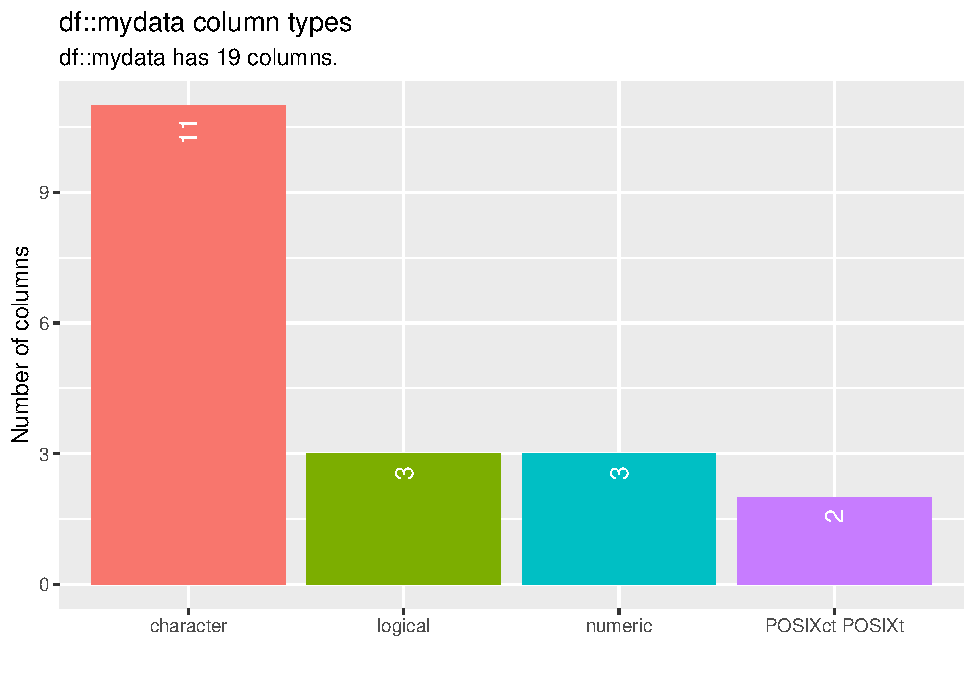
\includegraphics{/Users/serdarbalciold/histopathRprojects/histopathology-template/figs/variable type plot inspectdf-1.pdf}

\begin{Shaded}
\begin{Highlighting}[]
\CommentTok{# https://github.com/ropensci/visdat}
\CommentTok{# http://visdat.njtierney.com/articles/using_visdat.html}
\CommentTok{# https://cran.r-project.org/web/packages/visdat/index.html}
\CommentTok{# http://visdat.njtierney.com/}

\CommentTok{# visdat::vis_guess(mydata)}

\NormalTok{visdat}\OperatorTok{::}\KeywordTok{vis_dat}\NormalTok{(mydata)}
\end{Highlighting}
\end{Shaded}

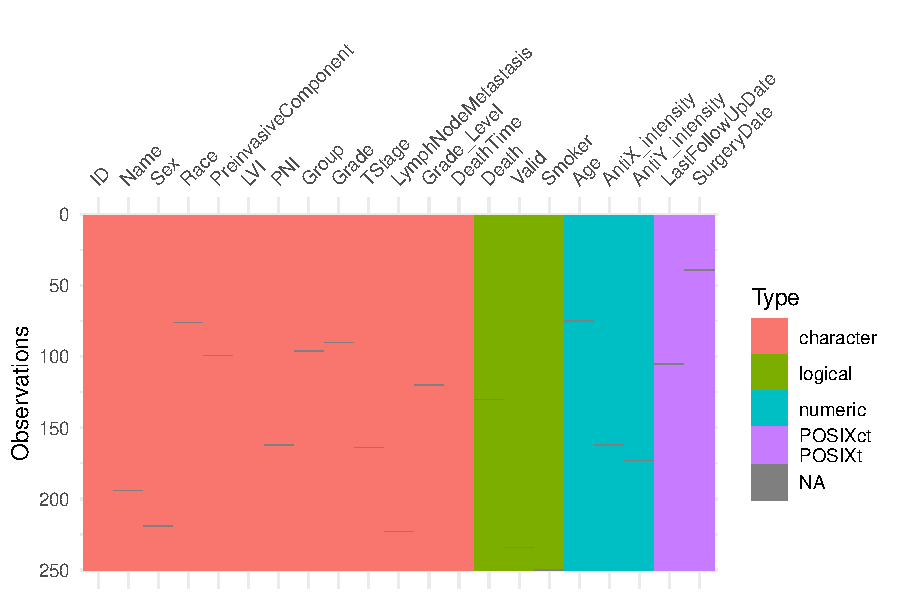
\includegraphics{/Users/serdarbalciold/histopathRprojects/histopathology-template/figs/variable type plot visdat-1.pdf}

\begin{Shaded}
\begin{Highlighting}[]
\NormalTok{mydata }\OperatorTok\StringTok{ }\NormalTok{explore}\OperatorTok{::}\KeywordTok{explore_tbl}\NormalTok{()}
\end{Highlighting}
\end{Shaded}

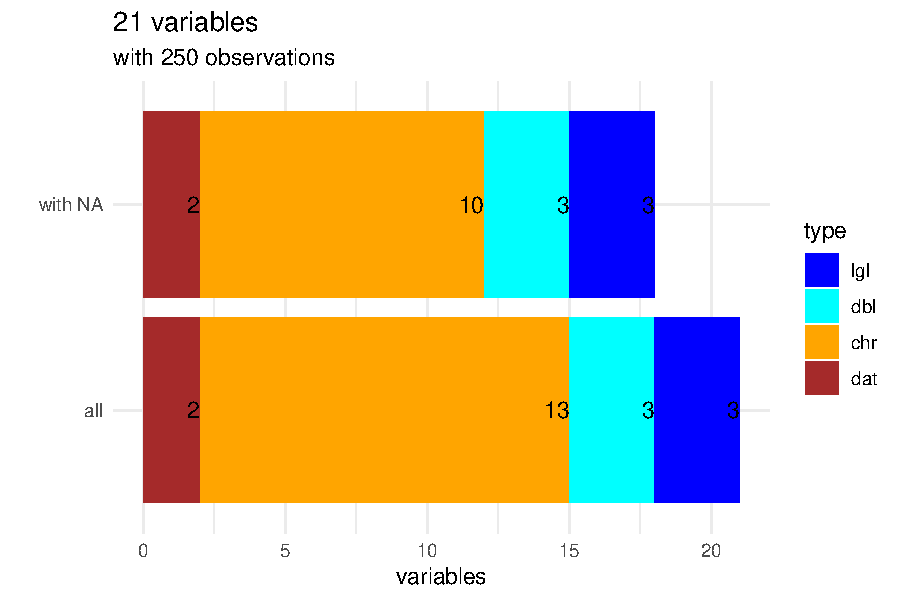
\includegraphics{/Users/serdarbalciold/histopathRprojects/histopathology-template/figs/variable type plot explore-1.pdf}

\hypertarget{define-variable-types-1}{%
\subsubsection{Define Variable Types}\label{define-variable-types-1}}

\hypertarget{find-character-variables}{%
\paragraph{\texorpdfstring{Find \texttt{character}
variables}{Find character variables}}\label{find-character-variables}}

\begin{Shaded}
\begin{Highlighting}[]
\NormalTok{characterVariables <-}\StringTok{ }\NormalTok{mydata }\OperatorTok\StringTok{ }\NormalTok{dplyr}\OperatorTok{::}\KeywordTok{select}\NormalTok{(}\OperatorTok{-}\NormalTok{keycolumns) }\OperatorTok\StringTok{ }\NormalTok{inspectdf}\OperatorTok{::}\KeywordTok{inspect_types}\NormalTok{() }\OperatorTok\StringTok{ }
\StringTok{    }\NormalTok{dplyr}\OperatorTok{::}\KeywordTok{filter}\NormalTok{(type }\OperatorTok{==}\StringTok{ "character"}\NormalTok{) }\OperatorTok\StringTok{ }\NormalTok{dplyr}\OperatorTok{::}\KeywordTok{select}\NormalTok{(col_name) }\OperatorTok\StringTok{ }\NormalTok{dplyr}\OperatorTok{::}\KeywordTok{pull}\NormalTok{() }\OperatorTok\StringTok{ }
\StringTok{    }\KeywordTok{unlist}\NormalTok{()}

\NormalTok{characterVariables}
\end{Highlighting}
\end{Shaded}

\begin{verbatim}
 [1] "Sex"                  "Race"                 "PreinvasiveComponent"
 [4] "LVI"                  "PNI"                  "Group"               
 [7] "Grade"                "TStage"               "LymphNodeMetastasis" 
[10] "Grade_Level"          "DeathTime"           
\end{verbatim}

\hypertarget{find-categorical-variables}{%
\paragraph{\texorpdfstring{Find \texttt{categorical}
variables}{Find categorical variables}}\label{find-categorical-variables}}

\begin{Shaded}
\begin{Highlighting}[]
\NormalTok{categoricalVariables <-}\StringTok{ }\NormalTok{mydata }\OperatorTok\StringTok{ }\NormalTok{dplyr}\OperatorTok{::}\KeywordTok{select}\NormalTok{(}\OperatorTok{-}\NormalTok{keycolumns, }\OperatorTok{-}\KeywordTok{contains}\NormalTok{(}\StringTok{"Date"}\NormalTok{)) }\OperatorTok\StringTok{ }
\StringTok{    }\NormalTok{describer}\OperatorTok{::}\KeywordTok{describe}\NormalTok{() }\OperatorTok\StringTok{ }\NormalTok{janitor}\OperatorTok{::}\KeywordTok{clean_names}\NormalTok{() }\OperatorTok\StringTok{ }\NormalTok{dplyr}\OperatorTok{::}\KeywordTok{filter}\NormalTok{(column_type }\OperatorTok{==}\StringTok{ }
\StringTok{    "factor"}\NormalTok{) }\OperatorTok\StringTok{ }\NormalTok{dplyr}\OperatorTok{::}\KeywordTok{select}\NormalTok{(column_name) }\OperatorTok\StringTok{ }\NormalTok{dplyr}\OperatorTok{::}\KeywordTok{pull}\NormalTok{()}

\NormalTok{categoricalVariables}
\end{Highlighting}
\end{Shaded}

\begin{verbatim}
character(0)
\end{verbatim}

\hypertarget{find-continious-variables}{%
\paragraph{\texorpdfstring{Find \texttt{continious}
variables}{Find continious variables}}\label{find-continious-variables}}

\begin{Shaded}
\begin{Highlighting}[]
\NormalTok{continiousVariables <-}\StringTok{ }\NormalTok{mydata }\OperatorTok\StringTok{ }\NormalTok{dplyr}\OperatorTok{::}\KeywordTok{select}\NormalTok{(}\OperatorTok{-}\NormalTok{keycolumns, }\OperatorTok{-}\KeywordTok{contains}\NormalTok{(}\StringTok{"Date"}\NormalTok{)) }\OperatorTok\StringTok{ }
\StringTok{    }\NormalTok{describer}\OperatorTok{::}\KeywordTok{describe}\NormalTok{() }\OperatorTok\StringTok{ }\NormalTok{janitor}\OperatorTok{::}\KeywordTok{clean_names}\NormalTok{() }\OperatorTok\StringTok{ }\NormalTok{dplyr}\OperatorTok{::}\KeywordTok{filter}\NormalTok{(column_type }\OperatorTok{==}\StringTok{ }
\StringTok{    "numeric"} \OperatorTok{|}\StringTok{ }\NormalTok{column_type }\OperatorTok{==}\StringTok{ "double"}\NormalTok{) }\OperatorTok\StringTok{ }\NormalTok{dplyr}\OperatorTok{::}\KeywordTok{select}\NormalTok{(column_name) }\OperatorTok\StringTok{ }\NormalTok{dplyr}\OperatorTok{::}\KeywordTok{pull}\NormalTok{()}

\NormalTok{continiousVariables}
\end{Highlighting}
\end{Shaded}

\begin{verbatim}
[1] "Age"             "AntiX_intensity" "AntiY_intensity"
\end{verbatim}

\hypertarget{find-numeric-variables}{%
\paragraph{\texorpdfstring{Find \texttt{numeric}
variables}{Find numeric variables}}\label{find-numeric-variables}}

\begin{Shaded}
\begin{Highlighting}[]
\NormalTok{numericVariables <-}\StringTok{ }\NormalTok{mydata }\OperatorTok\StringTok{ }\NormalTok{dplyr}\OperatorTok{::}\KeywordTok{select}\NormalTok{(}\OperatorTok{-}\NormalTok{keycolumns) }\OperatorTok\StringTok{ }\NormalTok{inspectdf}\OperatorTok{::}\KeywordTok{inspect_types}\NormalTok{() }\OperatorTok\StringTok{ }
\StringTok{    }\NormalTok{dplyr}\OperatorTok{::}\KeywordTok{filter}\NormalTok{(type }\OperatorTok{==}\StringTok{ "numeric"}\NormalTok{) }\OperatorTok\StringTok{ }\NormalTok{dplyr}\OperatorTok{::}\KeywordTok{select}\NormalTok{(col_name) }\OperatorTok\StringTok{ }\NormalTok{dplyr}\OperatorTok{::}\KeywordTok{pull}\NormalTok{() }\OperatorTok\StringTok{ }
\StringTok{    }\KeywordTok{unlist}\NormalTok{()}

\NormalTok{numericVariables}
\end{Highlighting}
\end{Shaded}

\begin{verbatim}
[1] "Age"             "AntiX_intensity" "AntiY_intensity"
\end{verbatim}

\hypertarget{find-integer-variables}{%
\paragraph{\texorpdfstring{Find \texttt{integer}
variables}{Find integer variables}}\label{find-integer-variables}}

\begin{Shaded}
\begin{Highlighting}[]
\NormalTok{integerVariables <-}\StringTok{ }\NormalTok{mydata }\OperatorTok\StringTok{ }\NormalTok{dplyr}\OperatorTok{::}\KeywordTok{select}\NormalTok{(}\OperatorTok{-}\NormalTok{keycolumns) }\OperatorTok\StringTok{ }\NormalTok{inspectdf}\OperatorTok{::}\KeywordTok{inspect_types}\NormalTok{() }\OperatorTok\StringTok{ }
\StringTok{    }\NormalTok{dplyr}\OperatorTok{::}\KeywordTok{filter}\NormalTok{(type }\OperatorTok{==}\StringTok{ "integer"}\NormalTok{) }\OperatorTok\StringTok{ }\NormalTok{dplyr}\OperatorTok{::}\KeywordTok{select}\NormalTok{(col_name) }\OperatorTok\StringTok{ }\NormalTok{dplyr}\OperatorTok{::}\KeywordTok{pull}\NormalTok{() }\OperatorTok\StringTok{ }
\StringTok{    }\KeywordTok{unlist}\NormalTok{()}

\NormalTok{integerVariables}
\end{Highlighting}
\end{Shaded}

\begin{verbatim}
NULL
\end{verbatim}

\hypertarget{find-list-variables}{%
\paragraph{\texorpdfstring{Find \texttt{list}
variables}{Find list variables}}\label{find-list-variables}}

\begin{Shaded}
\begin{Highlighting}[]
\NormalTok{listVariables <-}\StringTok{ }\NormalTok{mydata }\OperatorTok\StringTok{ }\NormalTok{dplyr}\OperatorTok{::}\KeywordTok{select}\NormalTok{(}\OperatorTok{-}\NormalTok{keycolumns) }\OperatorTok\StringTok{ }\NormalTok{inspectdf}\OperatorTok{::}\KeywordTok{inspect_types}\NormalTok{() }\OperatorTok\StringTok{ }
\StringTok{    }\NormalTok{dplyr}\OperatorTok{::}\KeywordTok{filter}\NormalTok{(type }\OperatorTok{==}\StringTok{ "list"}\NormalTok{) }\OperatorTok\StringTok{ }\NormalTok{dplyr}\OperatorTok{::}\KeywordTok{select}\NormalTok{(col_name) }\OperatorTok\StringTok{ }\NormalTok{dplyr}\OperatorTok{::}\KeywordTok{pull}\NormalTok{() }\OperatorTok\StringTok{ }
\StringTok{    }\KeywordTok{unlist}\NormalTok{()}
\NormalTok{listVariables}
\end{Highlighting}
\end{Shaded}

\begin{verbatim}
NULL
\end{verbatim}

\hypertarget{find-date-variables}{%
\paragraph{\texorpdfstring{Find \texttt{date}
variables}{Find date variables}}\label{find-date-variables}}

\begin{Shaded}
\begin{Highlighting}[]
\NormalTok{is_date <-}\StringTok{ }\ControlFlowTok{function}\NormalTok{(x) }\KeywordTok{inherits}\NormalTok{(x, }\KeywordTok{c}\NormalTok{(}\StringTok{"POSIXct"}\NormalTok{, }\StringTok{"POSIXt"}\NormalTok{))}

\NormalTok{dateVariables <-}\StringTok{ }\KeywordTok{names}\NormalTok{(}\KeywordTok{which}\NormalTok{(}\KeywordTok{sapply}\NormalTok{(mydata, }\DataTypeTok{FUN =}\NormalTok{ is_date) }\OperatorTok{==}\StringTok{ }\OtherTok{TRUE}\NormalTok{))}
\NormalTok{dateVariables}
\end{Highlighting}
\end{Shaded}

\begin{verbatim}
[1] "LastFollowUpDate" "SurgeryDate"     
\end{verbatim}

\begin{center}\rule{0.5\linewidth}{0.5pt}\end{center}

\hypertarget{overview-the-data}{%
\subsection{Overview the Data}\label{overview-the-data}}

\textbf{Codes for overviewing the data.}\footnote{See
  \href{https://github.com/sbalci/histopathology-template/blob/master/childRmd/_07overView.Rmd}{\texttt{childRmd/\_07overView.Rmd}}
  file for other codes}

\hypertarget{view-data}{%
\subsubsection{View Data}\label{view-data}}

\begin{Shaded}
\begin{Highlighting}[]
\KeywordTok{View}\NormalTok{(mydata)}
\end{Highlighting}
\end{Shaded}

\begin{Shaded}
\begin{Highlighting}[]
\NormalTok{reactable}\OperatorTok{::}\KeywordTok{reactable}\NormalTok{(}\DataTypeTok{data =}\NormalTok{ mydata, }\DataTypeTok{sortable =} \OtherTok{TRUE}\NormalTok{, }\DataTypeTok{resizable =} \OtherTok{TRUE}\NormalTok{, }\DataTypeTok{filterable =} \OtherTok{TRUE}\NormalTok{, }
    \DataTypeTok{searchable =} \OtherTok{TRUE}\NormalTok{, }\DataTypeTok{pagination =} \OtherTok{TRUE}\NormalTok{, }\DataTypeTok{paginationType =} \StringTok{"numbers"}\NormalTok{, }\DataTypeTok{showPageSizeOptions =} \OtherTok{TRUE}\NormalTok{, }
    \DataTypeTok{highlight =} \OtherTok{TRUE}\NormalTok{, }\DataTypeTok{striped =} \OtherTok{TRUE}\NormalTok{, }\DataTypeTok{outlined =} \OtherTok{TRUE}\NormalTok{, }\DataTypeTok{compact =} \OtherTok{TRUE}\NormalTok{, }\DataTypeTok{wrap =} \OtherTok{FALSE}\NormalTok{, }
    \DataTypeTok{showSortIcon =} \OtherTok{TRUE}\NormalTok{, }\DataTypeTok{showSortable =} \OtherTok{TRUE}\NormalTok{)}
\end{Highlighting}
\end{Shaded}

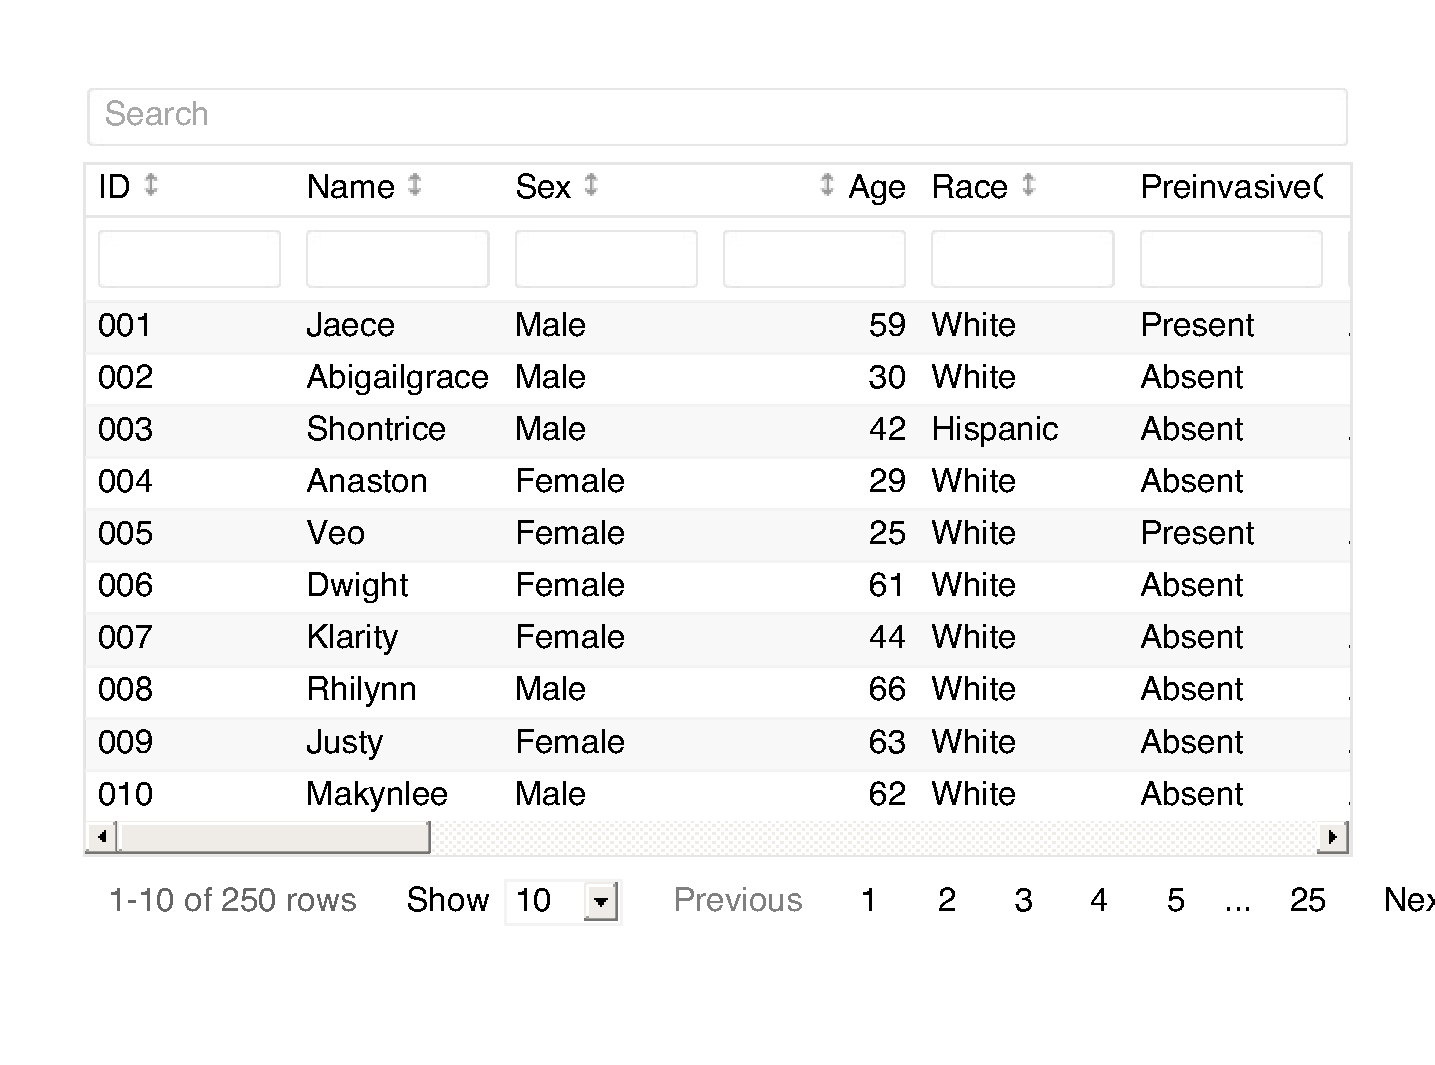
\includegraphics{/Users/serdarbalciold/histopathRprojects/histopathology-template/figs/view ractable-1.pdf}

\hypertarget{overview-exploratory-data-analysis-eda}{%
\subsubsection{Overview / Exploratory Data Analysis
(EDA)}\label{overview-exploratory-data-analysis-eda}}

\textbf{Summary of Data via summarytools 📦}

\begin{Shaded}
\begin{Highlighting}[]
\NormalTok{summarytools}\OperatorTok{::}\KeywordTok{view}\NormalTok{(summarytools}\OperatorTok{::}\KeywordTok{dfSummary}\NormalTok{(mydata }\OperatorTok\StringTok{ }\NormalTok{dplyr}\OperatorTok{::}\KeywordTok{select}\NormalTok{(}\OperatorTok{-}\NormalTok{keycolumns)))}
\end{Highlighting}
\end{Shaded}

\begin{Shaded}
\begin{Highlighting}[]
\ControlFlowTok{if}\NormalTok{ (}\OperatorTok{!}\KeywordTok{dir.exists}\NormalTok{(here}\OperatorTok{::}\KeywordTok{here}\NormalTok{(}\StringTok{"out"}\NormalTok{))) \{}
    \KeywordTok{dir.create}\NormalTok{(here}\OperatorTok{::}\KeywordTok{here}\NormalTok{(}\StringTok{"out"}\NormalTok{))}
\NormalTok{\}}

\NormalTok{summarytools}\OperatorTok{::}\KeywordTok{view}\NormalTok{(}\DataTypeTok{x =}\NormalTok{ summarytools}\OperatorTok{::}\KeywordTok{dfSummary}\NormalTok{(mydata }\OperatorTok\StringTok{ }\NormalTok{dplyr}\OperatorTok{::}\KeywordTok{select}\NormalTok{(}\OperatorTok{-}\NormalTok{keycolumns)), }
    \DataTypeTok{file =}\NormalTok{ here}\OperatorTok{::}\KeywordTok{here}\NormalTok{(}\StringTok{"out"}\NormalTok{, }\StringTok{"mydata_summary.html"}\NormalTok{))}
\end{Highlighting}
\end{Shaded}

\textbf{Summary via dataMaid 📦}

\begin{Shaded}
\begin{Highlighting}[]
\ControlFlowTok{if}\NormalTok{ (}\OperatorTok{!}\KeywordTok{dir.exists}\NormalTok{(here}\OperatorTok{::}\KeywordTok{here}\NormalTok{(}\StringTok{"out"}\NormalTok{))) \{}
    \KeywordTok{dir.create}\NormalTok{(here}\OperatorTok{::}\KeywordTok{here}\NormalTok{(}\StringTok{"out"}\NormalTok{))}
\NormalTok{\}}

\NormalTok{dataMaid}\OperatorTok{::}\KeywordTok{makeDataReport}\NormalTok{(}\DataTypeTok{data =}\NormalTok{ mydata, }\DataTypeTok{file =}\NormalTok{ here}\OperatorTok{::}\KeywordTok{here}\NormalTok{(}\StringTok{"out"}\NormalTok{, }\StringTok{"dataMaid_mydata.Rmd"}\NormalTok{), }
    \DataTypeTok{replace =} \OtherTok{TRUE}\NormalTok{, }\DataTypeTok{openResult =} \OtherTok{FALSE}\NormalTok{, }\DataTypeTok{render =} \OtherTok{FALSE}\NormalTok{, }\DataTypeTok{quiet =} \OtherTok{TRUE}\NormalTok{)}
\end{Highlighting}
\end{Shaded}

\textbf{Summary via explore 📦}

\begin{Shaded}
\begin{Highlighting}[]
\ControlFlowTok{if}\NormalTok{ (}\OperatorTok{!}\KeywordTok{dir.exists}\NormalTok{(here}\OperatorTok{::}\KeywordTok{here}\NormalTok{(}\StringTok{"out"}\NormalTok{))) \{}
    \KeywordTok{dir.create}\NormalTok{(here}\OperatorTok{::}\KeywordTok{here}\NormalTok{(}\StringTok{"out"}\NormalTok{))}
\NormalTok{\}}

\NormalTok{mydata }\OperatorTok\StringTok{ }\NormalTok{dplyr}\OperatorTok{::}\KeywordTok{select}\NormalTok{(}\OperatorTok{-}\NormalTok{dateVariables) }\OperatorTok\StringTok{ }\NormalTok{explore}\OperatorTok{::}\KeywordTok{report}\NormalTok{(}\DataTypeTok{output_file =} \StringTok{"mydata_report.html"}\NormalTok{, }
    \DataTypeTok{output_dir =}\NormalTok{ here}\OperatorTok{::}\KeywordTok{here}\NormalTok{(}\StringTok{"out"}\NormalTok{))}
\end{Highlighting}
\end{Shaded}

\textbf{Glimpse of Data}

\begin{Shaded}
\begin{Highlighting}[]
\NormalTok{dplyr}\OperatorTok{::}\KeywordTok{glimpse}\NormalTok{(mydata }\OperatorTok\StringTok{ }\NormalTok{dplyr}\OperatorTok{::}\KeywordTok{select}\NormalTok{(}\OperatorTok{-}\NormalTok{keycolumns, }\OperatorTok{-}\NormalTok{dateVariables))}
\end{Highlighting}
\end{Shaded}

\begin{verbatim}
Observations: 250
Variables: 17
$ Sex                  <chr> "Male", "Male", "Male", "Female", "Female", "F...
$ Age                  <dbl> 59, 30, 42, 29, 25, 61, 44, 66, 63, 62, 35, 43...
$ Race                 <chr> "White", "White", "Hispanic", "White", "White"...
$ PreinvasiveComponent <chr> "Present", "Absent", "Absent", "Absent", "Pres...
$ LVI                  <chr> "Absent", "Present", "Absent", "Present", "Abs...
$ PNI                  <chr> "Present", "Absent", "Absent", "Absent", "Pres...
$ Death                <lgl> TRUE, TRUE, TRUE, FALSE, TRUE, TRUE, TRUE, TRU...
$ Group                <chr> "Control", "Control", "Control", "Control", "C...
$ Grade                <chr> "2", "3", "1", "3", "3", "3", "3", "3", "3", "...
$ TStage               <chr> "3", "3", "4", "4", "2", "1", "2", "4", "2", "...
$ AntiX_intensity      <dbl> 2, 3, 3, 2, 2, 3, 3, 3, 3, 3, 2, 1, 3, 3, 3, 3...
$ AntiY_intensity      <dbl> 1, 2, 3, 2, 3, 3, 1, 3, 3, 1, 2, 3, 2, 2, 3, 3...
$ LymphNodeMetastasis  <chr> "Absent", "Absent", "Present", "Present", "Pre...
$ Valid                <lgl> FALSE, FALSE, TRUE, FALSE, FALSE, FALSE, TRUE,...
$ Smoker               <lgl> FALSE, FALSE, FALSE, FALSE, FALSE, TRUE, FALSE...
$ Grade_Level          <chr> "high", "moderate", "low", "moderate", "high",...
$ DeathTime            <chr> "Within1Year", "Within1Year", "Within1Year", "...
\end{verbatim}

\begin{Shaded}
\begin{Highlighting}[]
\NormalTok{mydata }\OperatorTok\StringTok{ }\NormalTok{explore}\OperatorTok{::}\KeywordTok{describe}\NormalTok{()}
\end{Highlighting}
\end{Shaded}

\begin{verbatim}
# A tibble: 21 x 8
   variable             type     na na_pct unique   min  mean   max
   <chr>                <chr> <int>  <dbl>  <int> <dbl> <dbl> <dbl>
 1 ID                   chr       0    0      250    NA NA       NA
 2 Name                 chr       1    0.4    250    NA NA       NA
 3 Sex                  chr       1    0.4      3    NA NA       NA
 4 Age                  dbl       1    0.4     49    25 49.0     73
 5 Race                 chr       1    0.4      8    NA NA       NA
 6 PreinvasiveComponent chr       1    0.4      3    NA NA       NA
 7 LVI                  chr       0    0        2    NA NA       NA
 8 PNI                  chr       1    0.4      3    NA NA       NA
 9 LastFollowUpDate     dat       1    0.4     13    NA NA       NA
10 Death                lgl       1    0.4      3     0  0.72     1
# ... with 11 more rows
\end{verbatim}

\textbf{Explore}

\begin{Shaded}
\begin{Highlighting}[]
\NormalTok{explore}\OperatorTok{::}\KeywordTok{explore}\NormalTok{(mydata)}
\end{Highlighting}
\end{Shaded}

\hypertarget{control-data}{%
\subsubsection{Control Data}\label{control-data}}

\textbf{Control Data if matching expectations}

\begin{Shaded}
\begin{Highlighting}[]
\NormalTok{visdat}\OperatorTok{::}\KeywordTok{vis_expect}\NormalTok{(}\DataTypeTok{data =}\NormalTok{ mydata, }\DataTypeTok{expectation =} \OperatorTok{~}\NormalTok{.x }\OperatorTok{==}\StringTok{ }\DecValTok{-1}\NormalTok{, }\DataTypeTok{show_perc =} \OtherTok{TRUE}\NormalTok{)}

\NormalTok{visdat}\OperatorTok{::}\KeywordTok{vis_expect}\NormalTok{(mydata, }\OperatorTok{~}\NormalTok{.x }\OperatorTok{>=}\StringTok{ }\DecValTok{25}\NormalTok{)}
\end{Highlighting}
\end{Shaded}

\textbf{See missing values}

\begin{Shaded}
\begin{Highlighting}[]
\NormalTok{visdat}\OperatorTok{::}\KeywordTok{vis_miss}\NormalTok{(airquality, }\DataTypeTok{cluster =} \OtherTok{TRUE}\NormalTok{)}
\end{Highlighting}
\end{Shaded}

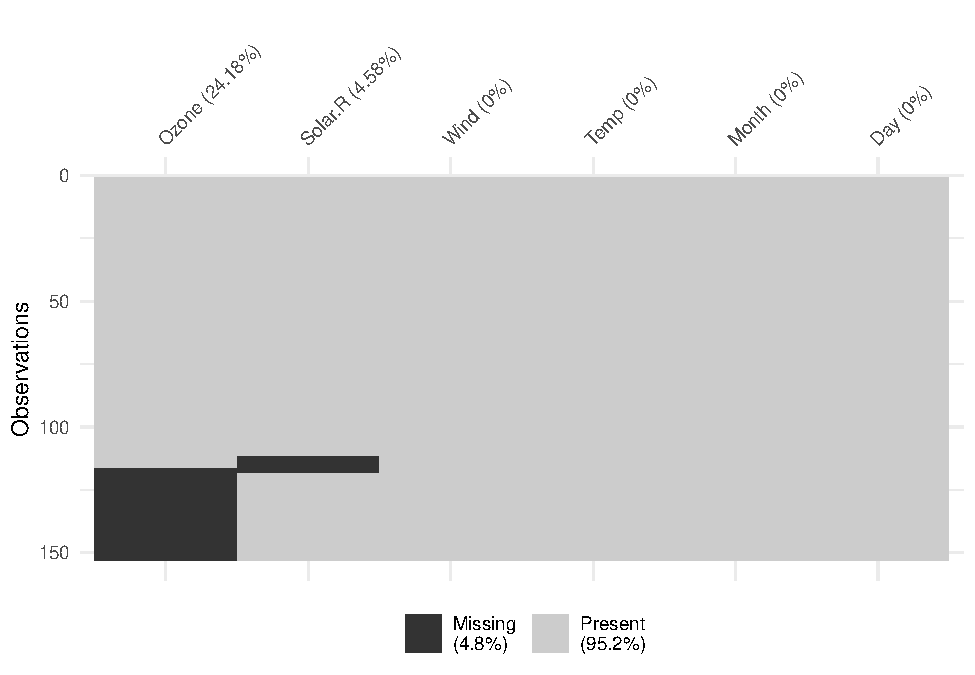
\includegraphics{/Users/serdarbalciold/histopathRprojects/histopathology-template/figs/missing values visdat-1.pdf}

\begin{Shaded}
\begin{Highlighting}[]
\NormalTok{visdat}\OperatorTok{::}\KeywordTok{vis_miss}\NormalTok{(airquality, }\DataTypeTok{sort_miss =} \OtherTok{TRUE}\NormalTok{)}
\end{Highlighting}
\end{Shaded}

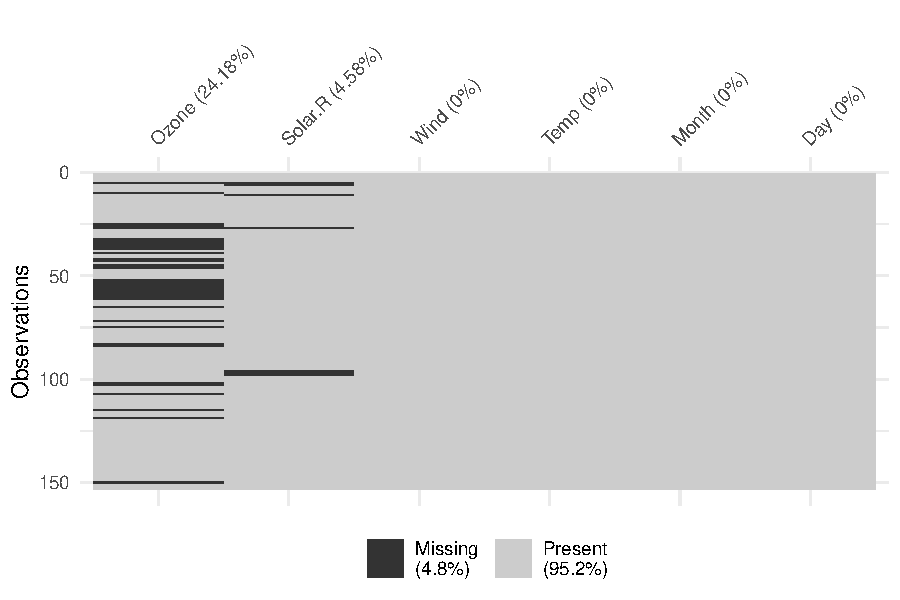
\includegraphics{/Users/serdarbalciold/histopathRprojects/histopathology-template/figs/missing values visdat 2-1.pdf}

\begin{Shaded}
\begin{Highlighting}[]
\NormalTok{xray}\OperatorTok{::}\KeywordTok{anomalies}\NormalTok{(mydata)}
\end{Highlighting}
\end{Shaded}

\begin{verbatim}
$variables
               Variable   q qNA  pNA qZero pZero qBlank pBlank qInf pInf
1                 Valid 250   1 0.4%   135   54%      0      -    0    -
2                Smoker 250   1 0.4%   132 52.8%      0      -    0    -
3                 Death 250   1 0.4%    69 27.6%      0      -    0    -
4                   Sex 250   1 0.4%     0     -      0      -    0    -
5  PreinvasiveComponent 250   1 0.4%     0     -      0      -    0    -
6                   PNI 250   1 0.4%     0     -      0      -    0    -
7                 Group 250   1 0.4%     0     -      0      -    0    -
8   LymphNodeMetastasis 250   1 0.4%     0     -      0      -    0    -
9                 Grade 250   1 0.4%     0     -      0      -    0    -
10      AntiX_intensity 250   1 0.4%     0     -      0      -    0    -
11      AntiY_intensity 250   1 0.4%     0     -      0      -    0    -
12          Grade_Level 250   1 0.4%     0     -      0      -    0    -
13               TStage 250   1 0.4%     0     -      0      -    0    -
14                 Race 250   1 0.4%     0     -      0      -    0    -
15     LastFollowUpDate 250   1 0.4%     0     -      0      -    0    -
16                  Age 250   1 0.4%     0     -      0      -    0    -
17          SurgeryDate 250   1 0.4%     0     -      0      -    0    -
18                 Name 250   1 0.4%     0     -      0      -    0    -
19                  LVI 250   0    -     0     -      0      -    0    -
20            DeathTime 250   0    -     0     -      0      -    0    -
21                   ID 250   0    -     0     -      0      -    0    -
   qDistinct      type anomalous_percent
1          3   Logical             54.4%
2          3   Logical             53.2%
3          3   Logical               28%
4          3 Character              0.4%
5          3 Character              0.4%
6          3 Character              0.4%
7          3 Character              0.4%
8          3 Character              0.4%
9          4 Character              0.4%
10         4   Numeric              0.4%
11         4   Numeric              0.4%
12         4 Character              0.4%
13         5 Character              0.4%
14         8 Character              0.4%
15        13 Timestamp              0.4%
16        49   Numeric              0.4%
17       233 Timestamp              0.4%
18       250 Character              0.4%
19         2 Character                 -
20         2 Character                 -
21       250 Character                 -

$problem_variables
 [1] Variable          q                 qNA               pNA              
 [5] qZero             pZero             qBlank            pBlank           
 [9] qInf              pInf              qDistinct         type             
[13] anomalous_percent problems         
<0 rows> (or 0-length row.names)
\end{verbatim}

\begin{Shaded}
\begin{Highlighting}[]
\NormalTok{xray}\OperatorTok{::}\KeywordTok{distributions}\NormalTok{(mydata)}
\end{Highlighting}
\end{Shaded}

\begin{verbatim}
================================================================================
\end{verbatim}

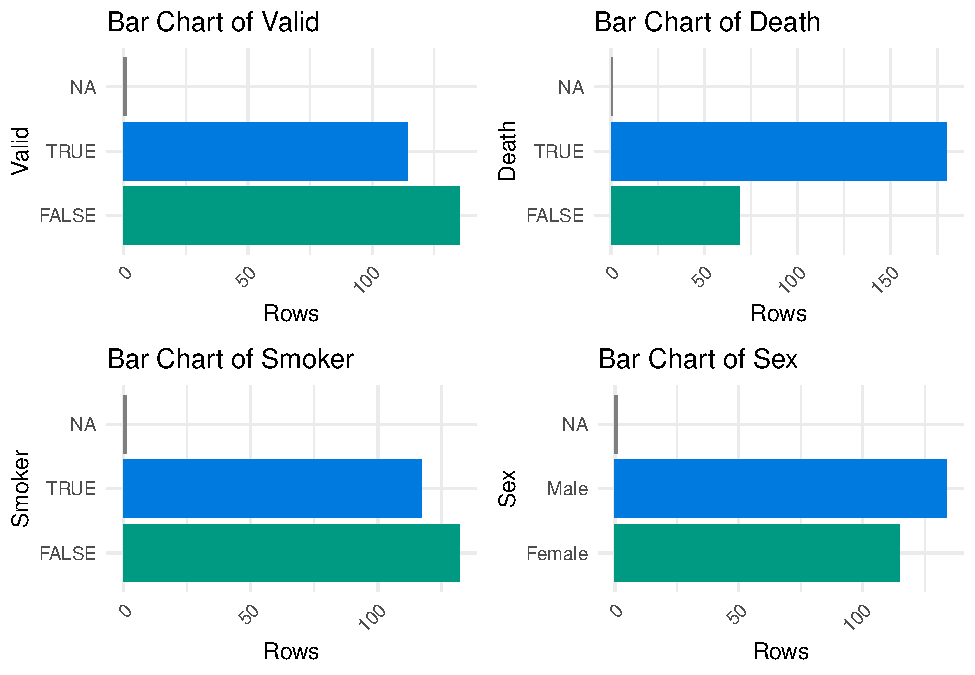
\includegraphics{/Users/serdarbalciold/histopathRprojects/histopathology-template/figs/xray 2-1.pdf}
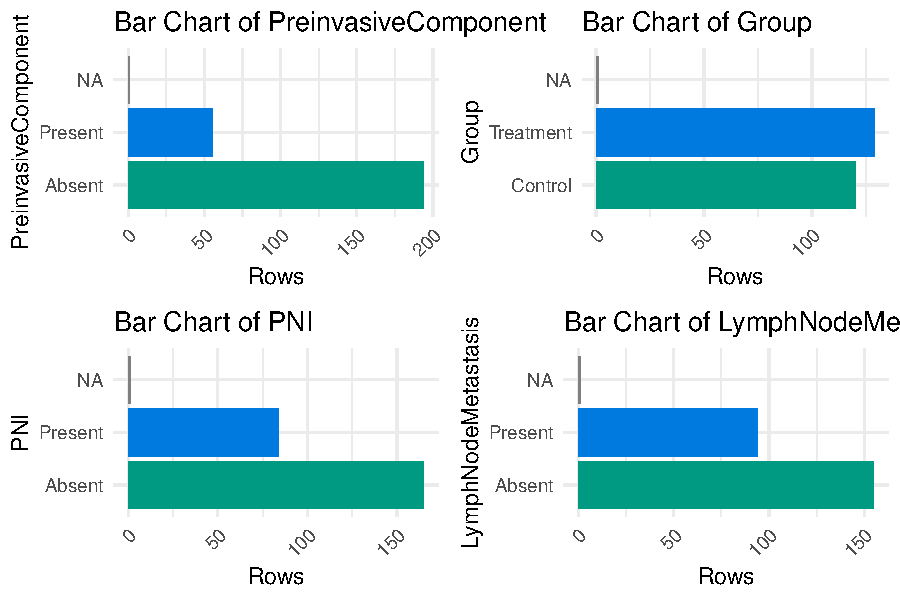
\includegraphics{/Users/serdarbalciold/histopathRprojects/histopathology-template/figs/xray 2-2.pdf}
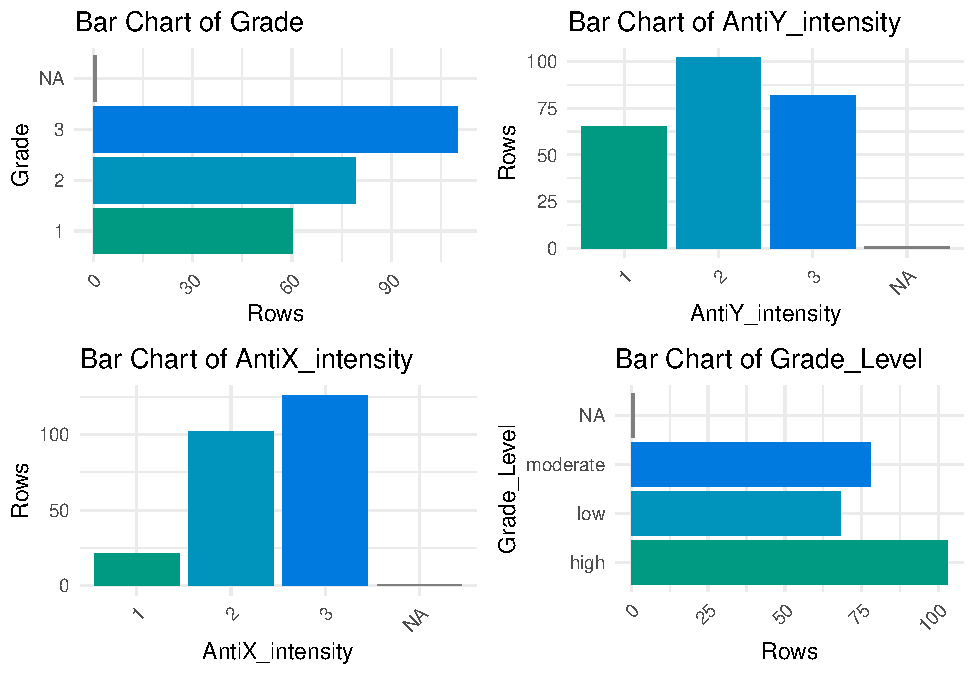
\includegraphics{/Users/serdarbalciold/histopathRprojects/histopathology-template/figs/xray 2-3.pdf}
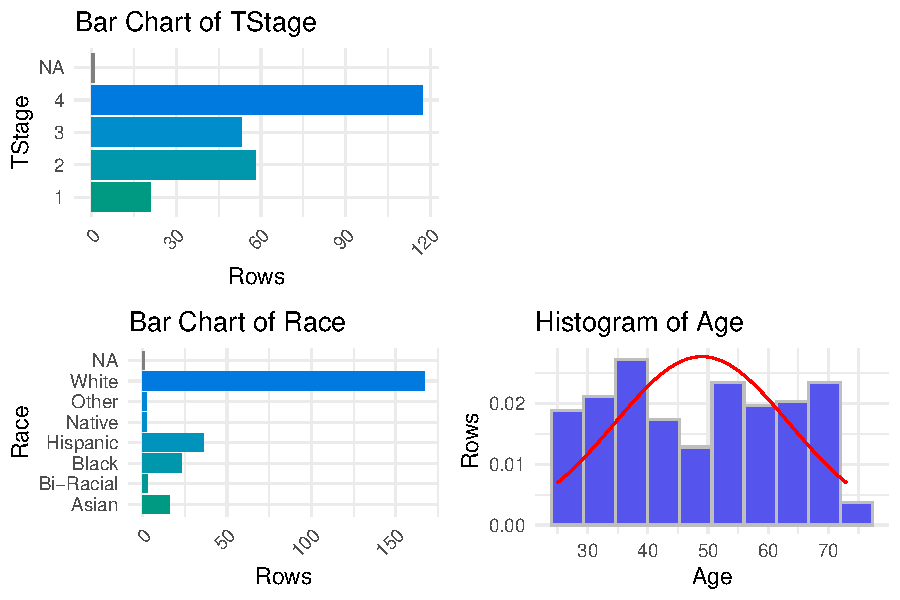
\includegraphics{/Users/serdarbalciold/histopathRprojects/histopathology-template/figs/xray 2-4.pdf}

\begin{verbatim}
[1] "Ignoring variable LastFollowUpDate: Unsupported type for visualization."
\end{verbatim}

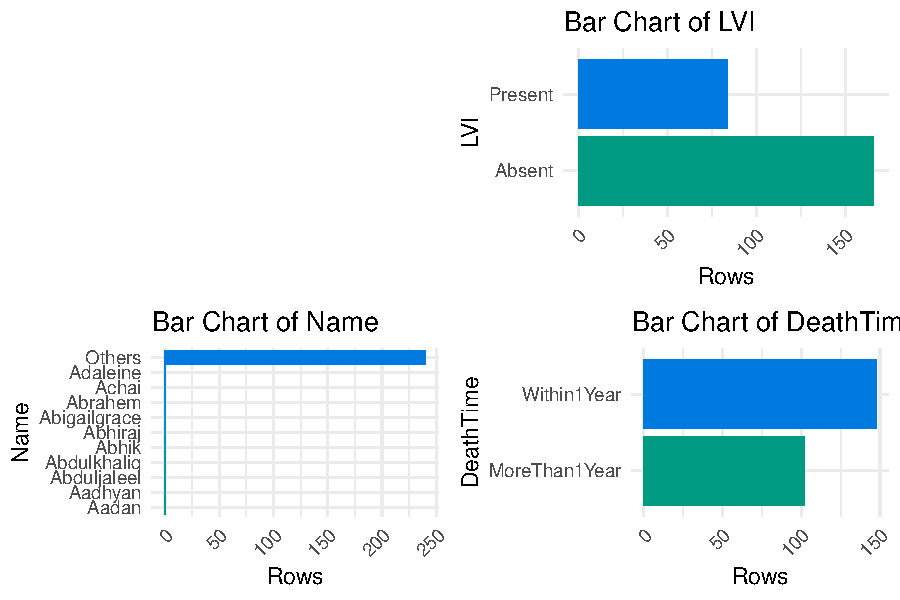
\includegraphics{/Users/serdarbalciold/histopathRprojects/histopathology-template/figs/xray 2-5.pdf}

\begin{verbatim}
[1] "Ignoring variable SurgeryDate: Unsupported type for visualization."
\end{verbatim}

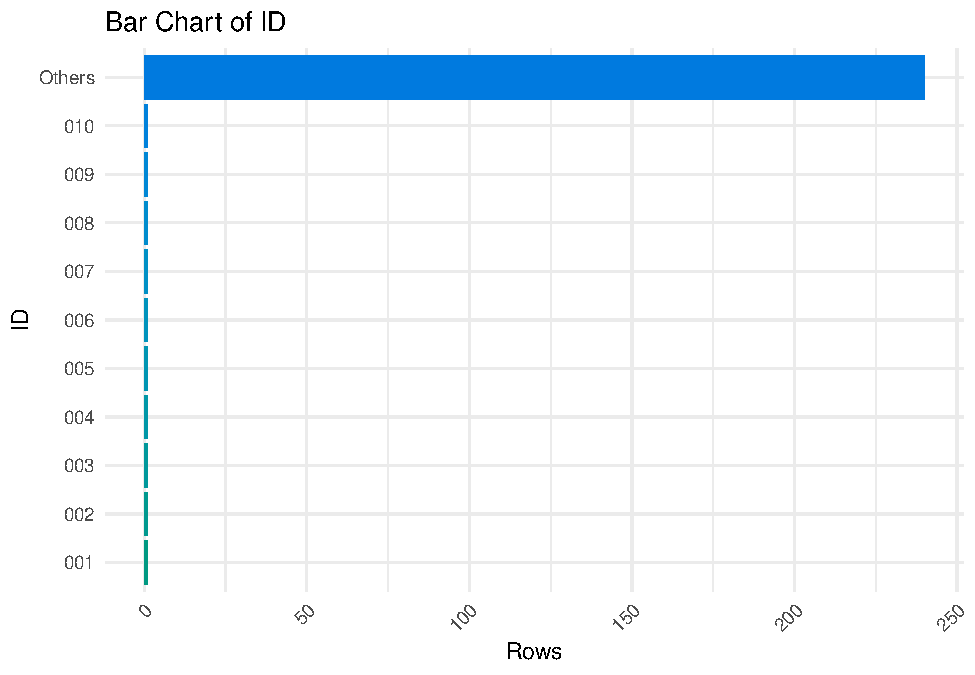
\includegraphics{/Users/serdarbalciold/histopathRprojects/histopathology-template/figs/xray 2-6.pdf}

\begin{verbatim}
         Variable p_1 p_10 p_25 p_50 p_75 p_90 p_99
1 AntiX_intensity   1    2    2    3    3    3    3
2 AntiY_intensity   1    1    1    2    3    3    3
3             Age  25 29.8   36   50   62 69.2   73
\end{verbatim}

\hypertarget{explore-data}{%
\subsubsection{Explore Data}\label{explore-data}}

\textbf{Summary of Data via DataExplorer 📦}

\begin{Shaded}
\begin{Highlighting}[]
\NormalTok{DataExplorer}\OperatorTok{::}\KeywordTok{plot_str}\NormalTok{(mydata)}
\end{Highlighting}
\end{Shaded}

\begin{Shaded}
\begin{Highlighting}[]
\NormalTok{DataExplorer}\OperatorTok{::}\KeywordTok{plot_str}\NormalTok{(mydata, }\DataTypeTok{type =} \StringTok{"r"}\NormalTok{)}
\end{Highlighting}
\end{Shaded}

\begin{Shaded}
\begin{Highlighting}[]
\NormalTok{DataExplorer}\OperatorTok{::}\KeywordTok{introduce}\NormalTok{(mydata)}
\end{Highlighting}
\end{Shaded}

\begin{verbatim}
# A tibble: 1 x 9
   rows columns discrete_columns continuous_colu~ all_missing_col~
  <int>   <int>            <int>            <int>            <int>
1   250      21               18                3                0
# ... with 4 more variables: total_missing_values <int>, complete_rows <int>,
#   total_observations <int>, memory_usage <dbl>
\end{verbatim}

\begin{Shaded}
\begin{Highlighting}[]
\NormalTok{DataExplorer}\OperatorTok{::}\KeywordTok{plot_intro}\NormalTok{(mydata)}
\end{Highlighting}
\end{Shaded}

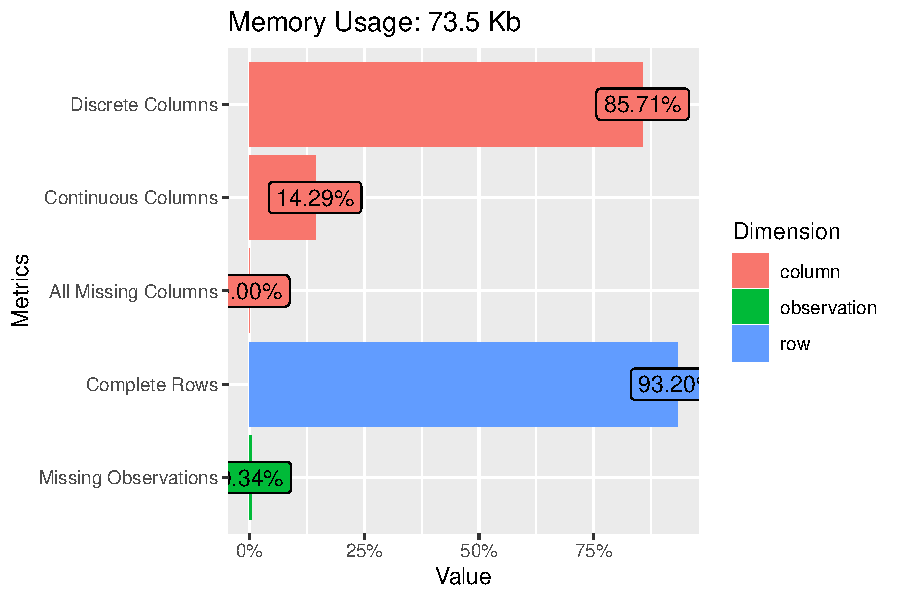
\includegraphics{/Users/serdarbalciold/histopathRprojects/histopathology-template/figs/DataExplorer 4-1.pdf}

\begin{Shaded}
\begin{Highlighting}[]
\NormalTok{DataExplorer}\OperatorTok{::}\KeywordTok{plot_missing}\NormalTok{(mydata)}
\end{Highlighting}
\end{Shaded}

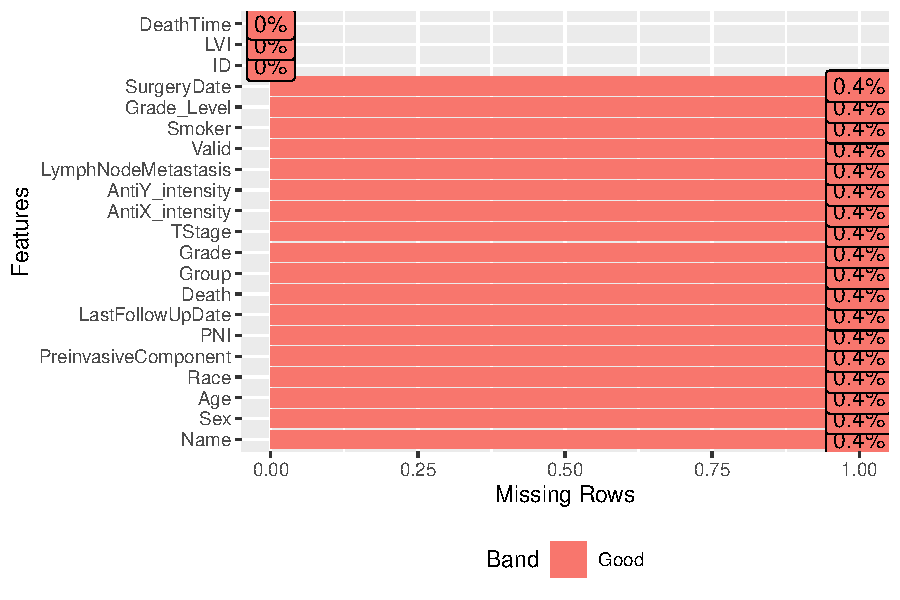
\includegraphics{/Users/serdarbalciold/histopathRprojects/histopathology-template/figs/DataExplorer 5-1.pdf}

\textbf{Drop columns}

\begin{Shaded}
\begin{Highlighting}[]
\NormalTok{mydata2 <-}\StringTok{ }\NormalTok{DataExplorer}\OperatorTok{::}\KeywordTok{drop_columns}\NormalTok{(mydata, }\StringTok{"TStage"}\NormalTok{)}
\end{Highlighting}
\end{Shaded}

\begin{Shaded}
\begin{Highlighting}[]
\NormalTok{DataExplorer}\OperatorTok{::}\KeywordTok{plot_bar}\NormalTok{(mydata)}
\end{Highlighting}
\end{Shaded}

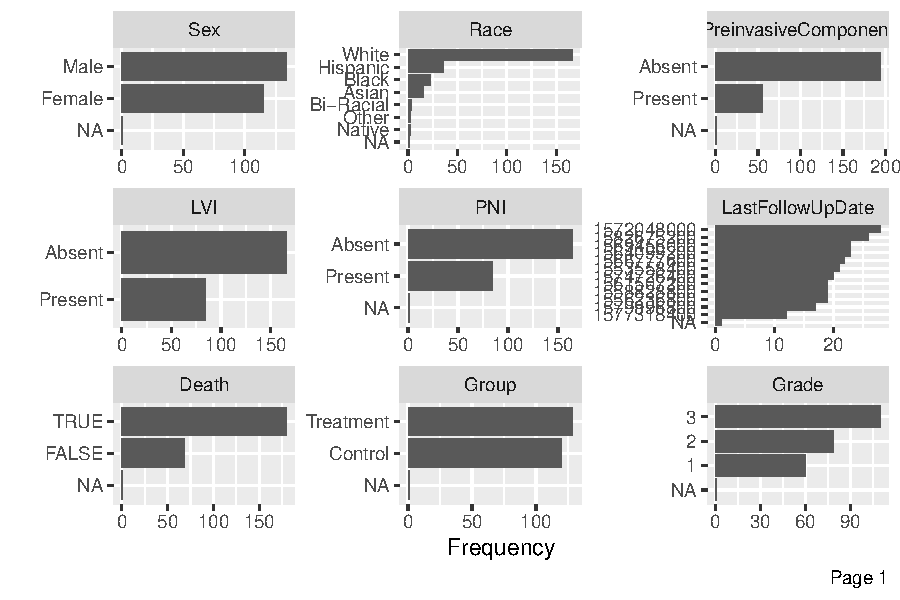
\includegraphics{/Users/serdarbalciold/histopathRprojects/histopathology-template/figs/DataExplorer 7-1.pdf}
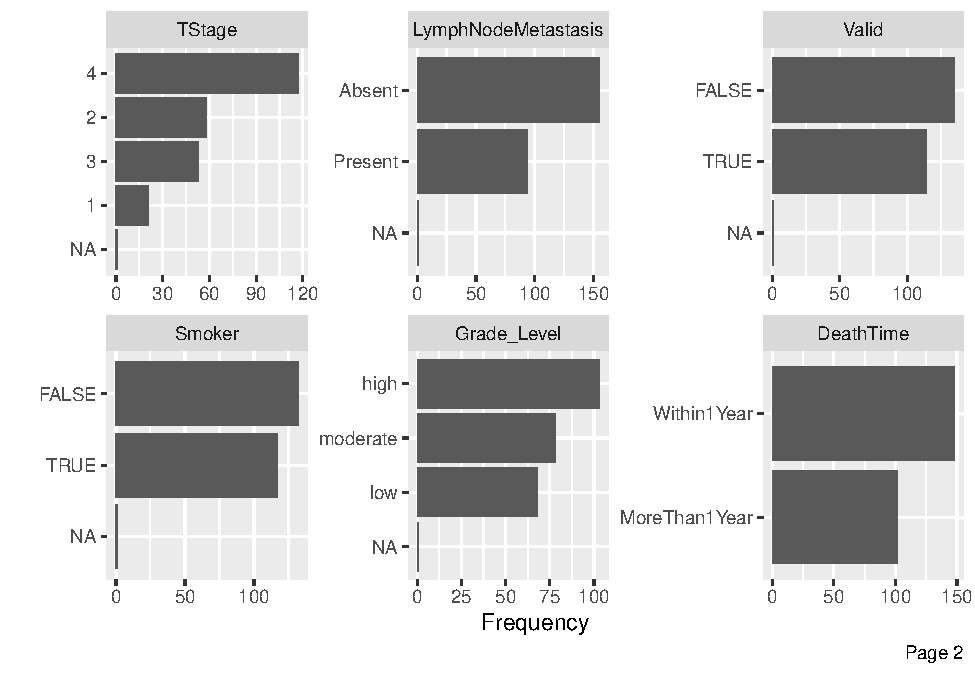
\includegraphics{/Users/serdarbalciold/histopathRprojects/histopathology-template/figs/DataExplorer 7-2.pdf}

\begin{Shaded}
\begin{Highlighting}[]
\NormalTok{DataExplorer}\OperatorTok{::}\KeywordTok{plot_bar}\NormalTok{(mydata, }\DataTypeTok{with =} \StringTok{"Death"}\NormalTok{)}
\end{Highlighting}
\end{Shaded}

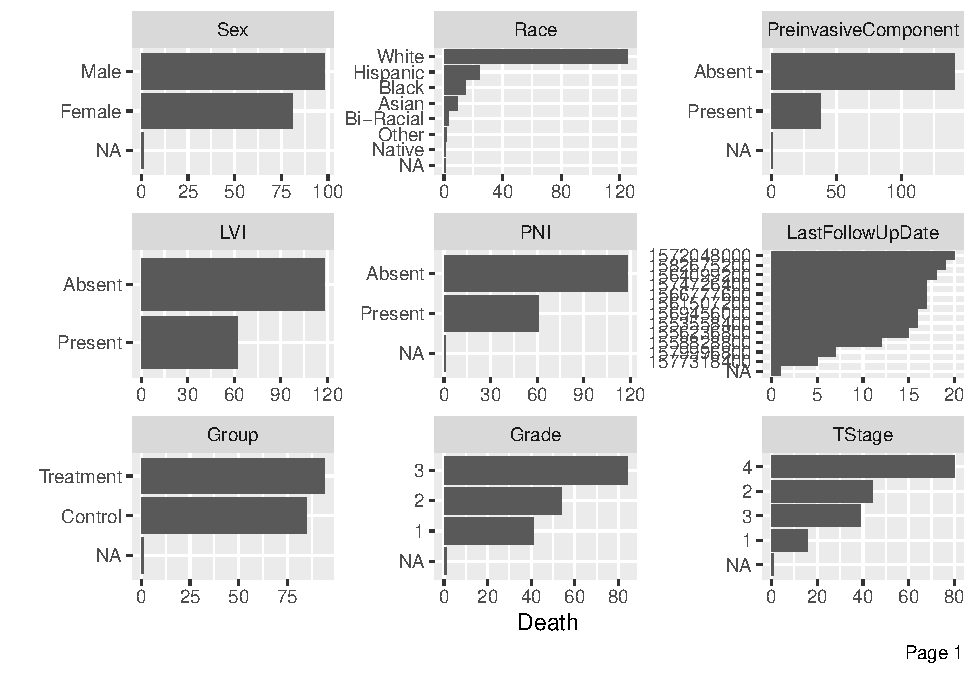
\includegraphics{/Users/serdarbalciold/histopathRprojects/histopathology-template/figs/DataExplorer 8-1.pdf}
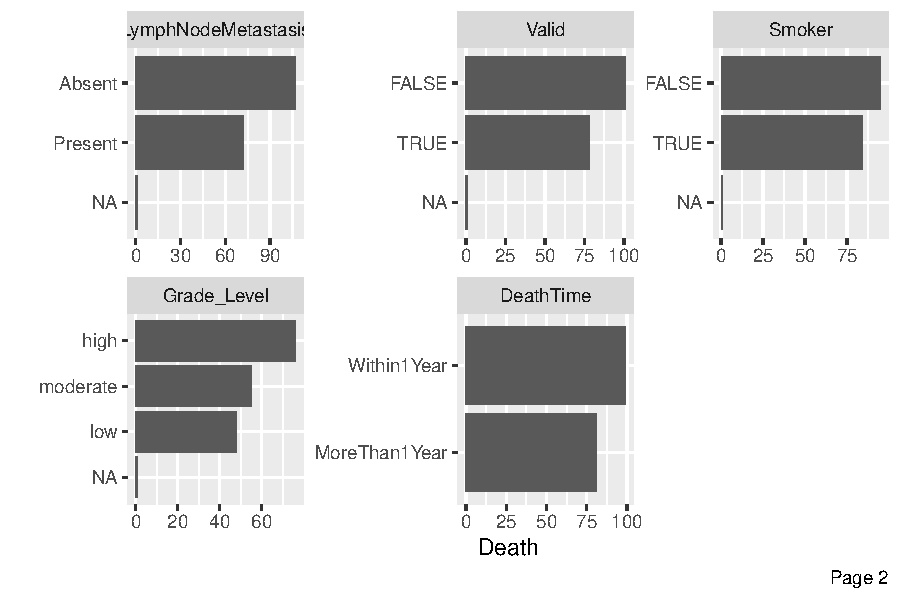
\includegraphics{/Users/serdarbalciold/histopathRprojects/histopathology-template/figs/DataExplorer 8-2.pdf}

\begin{Shaded}
\begin{Highlighting}[]
\NormalTok{DataExplorer}\OperatorTok{::}\KeywordTok{plot_histogram}\NormalTok{(mydata)}
\end{Highlighting}
\end{Shaded}

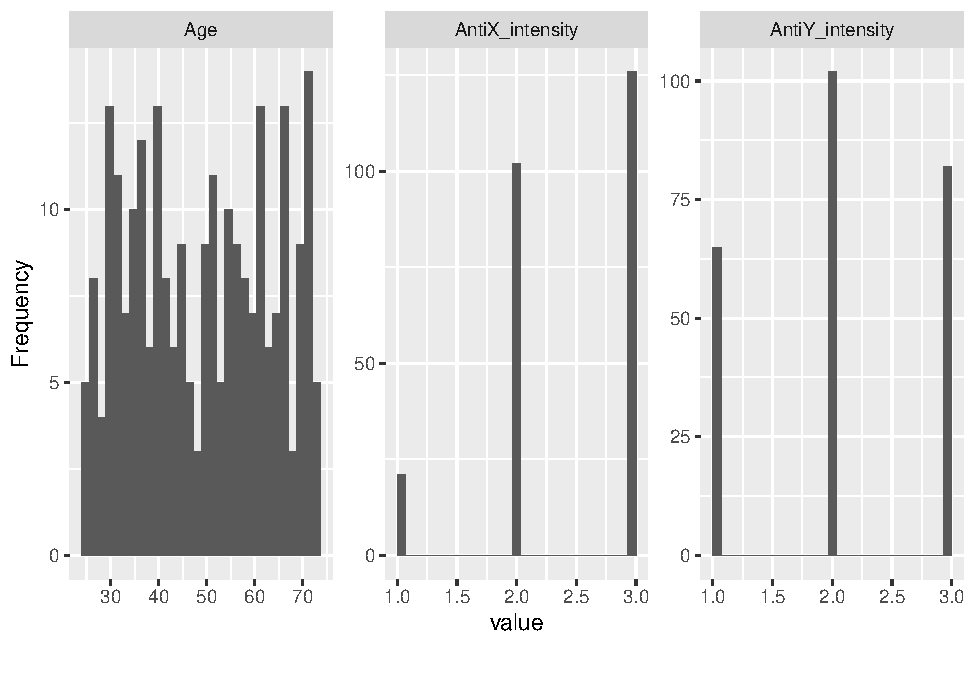
\includegraphics{/Users/serdarbalciold/histopathRprojects/histopathology-template/figs/DataExplorer 9-1.pdf}

\begin{center}\rule{0.5\linewidth}{0.5pt}\end{center}

\begin{center}\rule{0.5\linewidth}{0.5pt}\end{center}

\hypertarget{statistical-analysis}{%
\section{Statistical Analysis}\label{statistical-analysis}}

\textbf{Learn these tests as highlighted in (Schmidt et al.
2017).}\footnote{Statistical Literacy Among Academic Pathologists: A
  Survey Study to Gauge Knowledge of Frequently Used Statistical Tests
  Among Trainees and Faculty. Archives of Pathology \& Laboratory
  Medicine: February 2017, Vol. 141, No.~2, pp.~279-287.
  \url{https://doi.org/10.5858/arpa.2016-0200-OA}}

\begin{center}\rule{0.5\linewidth}{0.5pt}\end{center}

\hypertarget{results}{%
\section{Results}\label{results}}

\textbf{Write results as described in (Knijn, Simmer, and Nagtegaal
2015)}\footnote{From Table 1: Proposed items for reporting
  histopathology studies. Recommendations for reporting histopathology
  studies: a proposal Virchows Arch (2015) 466:611--615 DOI
  10.1007/s00428-015-1762-3
  \url{https://www.ncbi.nlm.nih.gov/pmc/articles/PMC4460276/}}

\begin{itemize}
\item
  Describe the number of patients included in the analysis and reason
  for dropout
\item
  Report patient/disease characteristics (including the biomarker of
  interest) with the number of missing values
\item
  Describe the interaction of the biomarker of interest with established
  prognostic variables
\item
  Include at least 90 \% of initial cases included in univariate and
  multivariate analyses
\item
  Report the estimated effect (relative risk/odds ratio, confidence
  interval, and p value) in univariate analysis
\item
  Report the estimated effect (hazard rate/odds ratio, confidence
  interval, and p value) in multivariate analysis
\item
  Report the estimated effects (hazard ratio/odds ratio, confidence
  interval, and p value) of other prognostic factors included in
  multivariate analysis
\end{itemize}

\begin{center}\rule{0.5\linewidth}{0.5pt}\end{center}

\hypertarget{data-dictionary}{%
\subsection{Data Dictionary}\label{data-dictionary}}

\textbf{Codes for generating data dictionary}.\footnote{See
  \href{https://github.com/sbalci/histopathology-template/blob/master/childRmd/_08dataDictionary.Rmd}{\texttt{childRmd/\_08dataDictionary.Rmd}}
  file for other codes}

\begin{center}\rule{0.5\linewidth}{0.5pt}\end{center}

\hypertarget{clean-and-recode-data}{%
\subsection{Clean and Recode Data}\label{clean-and-recode-data}}

\textbf{Codes for clean and recode data}.\footnote{See
  \href{https://github.com/sbalci/histopathology-template/blob/master/childRmd/_09cleanRecode.Rmd}{\texttt{childRmd/\_09cleanRecode.Rmd}}
  file for other codes}

questionr::irec()

questionr::iorder()

questionr::icut()

iris \%\textgreater\% mutate(sumVar = rowSums(.{[}1:4{]}))

iris \%\textgreater\% mutate(sumVar = rowSums(select(.,
contains(``Sepal'')))) \%\textgreater\% head

iris \%\textgreater\% mutate(sumVar = select(., contains(``Sepal''))
\%\textgreater\% rowSums()) \%\textgreater\% head

iRenameColumn.R

iSelectColumn.R

\begin{verbatim}
<= 22 Low
>= 23 & <= 41 Average 
>=42 High
\end{verbatim}

\begin{center}\rule{0.5\linewidth}{0.5pt}\end{center}

\hypertarget{impute-missing-data}{%
\subsection{Impute Missing Data}\label{impute-missing-data}}

\hypertarget{impute}{%
\subsection{impute}\label{impute}}

\textbf{Codes for missing data and impute}.\footnote{See
  \href{https://github.com/sbalci/histopathology-template/blob/master/childRmd/_10impute.Rmd}{\texttt{childRmd/\_10impute.Rmd}}
  file for other codes}

\begin{itemize}
\item
  Multiple imputation support in Finalfit\\
  \url{https://www.datasurg.net/2019/09/25/multiple-imputation-support-in-finalfit/}
\item
  Missing data\\
  \url{https://finalfit.org/articles/missing.html}
\end{itemize}

\hypertarget{missing-data}{%
\subsubsection{Missing Data}\label{missing-data}}

\textbf{Plot missing data}

\begin{Shaded}
\begin{Highlighting}[]
\NormalTok{visdat}\OperatorTok{::}\KeywordTok{vis_miss}\NormalTok{(mydata)}
\end{Highlighting}
\end{Shaded}

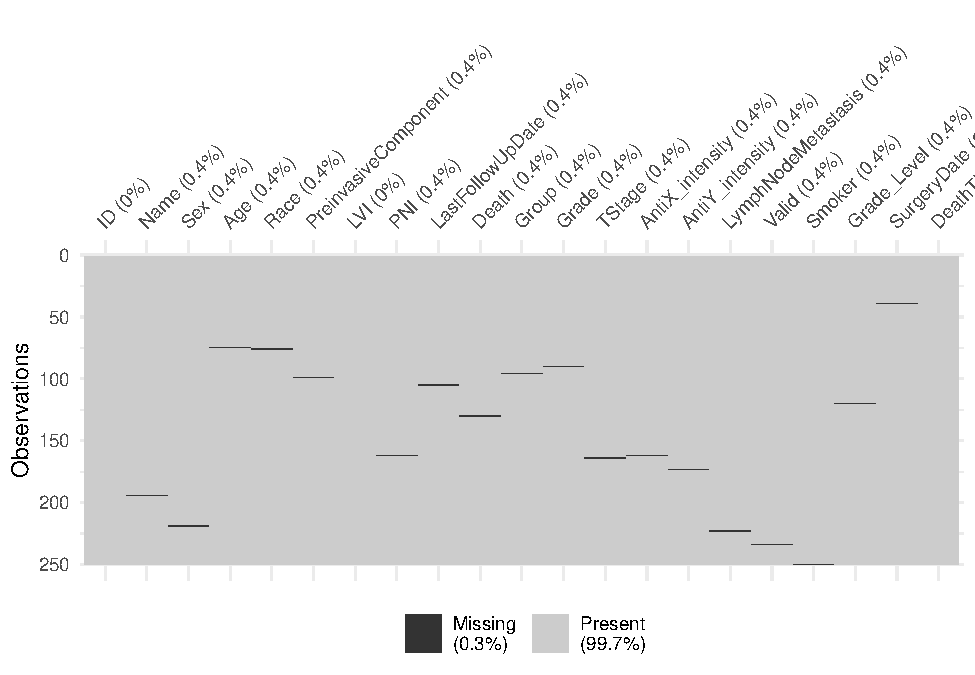
\includegraphics{/Users/serdarbalciold/histopathRprojects/histopathology-template/figs/visdat-1.pdf}

\hypertarget{impute-continious}{%
\subsubsection{impute continious}\label{impute-continious}}

\hypertarget{impute-categorical}{%
\subsubsection{impute categorical}\label{impute-categorical}}

\hypertarget{impute-outlier}{%
\subsubsection{impute outlier}\label{impute-outlier}}

\hypertarget{transform}{%
\subsection{transform}\label{transform}}

\hypertarget{min--max}{%
\subsubsection{min -max}\label{min--max}}

\hypertarget{skewness}{%
\subsubsection{skewness}\label{skewness}}

\hypertarget{log}{%
\subsubsection{log}\label{log}}

\hypertarget{binning}{%
\subsection{binning}\label{binning}}

\hypertarget{optimal-binning}{%
\subsubsection{optimal binning}\label{optimal-binning}}

\hypertarget{standardize}{%
\subsubsection{standardize}\label{standardize}}

\hypertarget{data-transformation-report}{%
\subsection{data transformation
report}\label{data-transformation-report}}

\hypertarget{inspectdf}{%
\subsection{inspectdf}\label{inspectdf}}

\begin{center}\rule{0.5\linewidth}{0.5pt}\end{center}

\pagebreak

\hypertarget{descriptive-statistics}{%
\subsection{Descriptive Statistics}\label{descriptive-statistics}}

\textbf{Codes for Descriptive Statistics}.\footnote{See
  \href{https://github.com/sbalci/histopathology-template/blob/master/childRmd/_11descriptives.Rmd}{\texttt{childRmd/\_11descriptives.Rmd}}
  file for other codes}

\hypertarget{table-one}{%
\subsubsection{Table One}\label{table-one}}

\textbf{Report Data properties via report 📦}

\begin{Shaded}
\begin{Highlighting}[]
\NormalTok{mydata }\OperatorTok\StringTok{ }\NormalTok{dplyr}\OperatorTok{::}\KeywordTok{select}\NormalTok{(}\OperatorTok{-}\NormalTok{dplyr}\OperatorTok{::}\KeywordTok{contains}\NormalTok{(}\StringTok{"Date"}\NormalTok{)) }\OperatorTok\StringTok{ }\NormalTok{report}\OperatorTok{::}\KeywordTok{report}\NormalTok{()}
\end{Highlighting}
\end{Shaded}

\begin{verbatim}
The data contains 250 observations of the following variables:
  - ID: 250 entries: 001, n = 1; 002, n = 1; 003, n = 1 and 247 others (0 missing)
  - Name: 249 entries: Aadan, n = 1; Aadhyan, n = 1; Abduljaleel, n = 1 and 246 others (1 missing)
  - Sex: 2 entries: Male, n = 134; Female, n = 115 (1 missing)
  - Age: Mean = 48.99, SD = 14.44, Median = , MAD = 19.27, range: [25, 73], Skewness = 0.03, Kurtosis = -1.28, 1 missing
  - Race: 7 entries: White, n = 167; Hispanic, n = 36; Black, n = 23 and 4 others (1 missing)
  - PreinvasiveComponent: 2 entries: Absent, n = 194; Present, n = 55 (1 missing)
  - LVI: 2 entries: Absent, n = 166; Present, n = 84 (0 missing)
  - PNI: 2 entries: Absent, n = 165; Present, n = 84 (1 missing)
  - Death: 2 levels: FALSE (n = 69, 27.60%); TRUE (n = 180, 72.00%) and missing (n = 1, 0.40%)
  - Group: 2 entries: Treatment, n = 129; Control, n = 120 (1 missing)
  - Grade: 3 entries: 3, n = 110; 2, n = 79; 1, n = 60 (1 missing)
  - TStage: 4 entries: 4, n = 117; 2, n = 58; 3, n = 53 and 1 other (1 missing)
  - AntiX_intensity: Mean = 2.42, SD = 0.64, Median = , MAD = 0.00, range: [1, 3], Skewness = -0.67, Kurtosis = -0.57, 1 missing
  - AntiY_intensity: Mean = 2.07, SD = 0.77, Median = , MAD = 1.48, range: [1, 3], Skewness = -0.12, Kurtosis = -1.29, 1 missing
  - LymphNodeMetastasis: 2 entries: Absent, n = 155; Present, n = 94 (1 missing)
  - Valid: 2 levels: FALSE (n = 135, 54.00%); TRUE (n = 114, 45.60%) and missing (n = 1, 0.40%)
  - Smoker: 2 levels: FALSE (n = 132, 52.80%); TRUE (n = 117, 46.80%) and missing (n = 1, 0.40%)
  - Grade_Level: 3 entries: high, n = 103; moderate, n = 78; low, n = 68 (1 missing)
  - DeathTime: 2 entries: Within1Year, n = 148; MoreThan1Year, n = 102 (0 missing)
\end{verbatim}

\textbf{Table 1 via arsenal 📦}

\begin{Shaded}
\begin{Highlighting}[]
\CommentTok{# cat(names(mydata), sep = " + \textbackslash{}n")}
\KeywordTok{library}\NormalTok{(arsenal)}
\NormalTok{tab1 <-}\StringTok{ }\NormalTok{arsenal}\OperatorTok{::}\KeywordTok{tableby}\NormalTok{(}
  \OperatorTok{~}\StringTok{ }\NormalTok{Sex }\OperatorTok{+}
\StringTok{    }\NormalTok{Age }\OperatorTok{+}
\StringTok{    }\NormalTok{Race }\OperatorTok{+}
\StringTok{    }\NormalTok{PreinvasiveComponent }\OperatorTok{+}
\StringTok{    }\NormalTok{LVI }\OperatorTok{+}
\StringTok{    }\NormalTok{PNI }\OperatorTok{+}
\StringTok{    }\NormalTok{Death }\OperatorTok{+}
\StringTok{    }\NormalTok{Group }\OperatorTok{+}
\StringTok{    }\NormalTok{Grade }\OperatorTok{+}
\StringTok{    }\NormalTok{TStage }\OperatorTok{+}
\StringTok{    }\CommentTok{# `Anti-X-intensity` +}
\StringTok{    }\CommentTok{# `Anti-Y-intensity` +}
\StringTok{    }\NormalTok{LymphNodeMetastasis }\OperatorTok{+}
\StringTok{    }\NormalTok{Valid }\OperatorTok{+}
\StringTok{    }\NormalTok{Smoker }\OperatorTok{+}
\StringTok{    }\NormalTok{Grade_Level}
\NormalTok{  ,}
  \DataTypeTok{data =}\NormalTok{ mydata }
\NormalTok{)}
\KeywordTok{summary}\NormalTok{(tab1)}
\end{Highlighting}
\end{Shaded}

\begin{longtable}[]{@{}lc@{}}
\toprule
& Overall (N=250)\tabularnewline
\midrule
\endhead
\textbf{Sex} &\tabularnewline
~~~N-Miss & 1\tabularnewline
~~~Female & 115 (46.2\%)\tabularnewline
~~~Male & 134 (53.8\%)\tabularnewline
\textbf{Age} &\tabularnewline
~~~N-Miss & 1\tabularnewline
~~~Mean (SD) & 48.992 (14.442)\tabularnewline
~~~Range & 25.000 - 73.000\tabularnewline
\textbf{Race} &\tabularnewline
~~~N-Miss & 1\tabularnewline
~~~Asian & 16 (6.4\%)\tabularnewline
~~~Bi-Racial & 3 (1.2\%)\tabularnewline
~~~Black & 23 (9.2\%)\tabularnewline
~~~Hispanic & 36 (14.5\%)\tabularnewline
~~~Native & 2 (0.8\%)\tabularnewline
~~~Other & 2 (0.8\%)\tabularnewline
~~~White & 167 (67.1\%)\tabularnewline
\textbf{PreinvasiveComponent} &\tabularnewline
~~~N-Miss & 1\tabularnewline
~~~Absent & 194 (77.9\%)\tabularnewline
~~~Present & 55 (22.1\%)\tabularnewline
\textbf{LVI} &\tabularnewline
~~~Absent & 166 (66.4\%)\tabularnewline
~~~Present & 84 (33.6\%)\tabularnewline
\textbf{PNI} &\tabularnewline
~~~N-Miss & 1\tabularnewline
~~~Absent & 165 (66.3\%)\tabularnewline
~~~Present & 84 (33.7\%)\tabularnewline
\textbf{Death} &\tabularnewline
~~~N-Miss & 1\tabularnewline
~~~FALSE & 69 (27.7\%)\tabularnewline
~~~TRUE & 180 (72.3\%)\tabularnewline
\textbf{Group} &\tabularnewline
~~~N-Miss & 1\tabularnewline
~~~Control & 120 (48.2\%)\tabularnewline
~~~Treatment & 129 (51.8\%)\tabularnewline
\textbf{Grade} &\tabularnewline
~~~N-Miss & 1\tabularnewline
~~~1 & 60 (24.1\%)\tabularnewline
~~~2 & 79 (31.7\%)\tabularnewline
~~~3 & 110 (44.2\%)\tabularnewline
\textbf{TStage} &\tabularnewline
~~~N-Miss & 1\tabularnewline
~~~1 & 21 (8.4\%)\tabularnewline
~~~2 & 58 (23.3\%)\tabularnewline
~~~3 & 53 (21.3\%)\tabularnewline
~~~4 & 117 (47.0\%)\tabularnewline
\textbf{LymphNodeMetastasis} &\tabularnewline
~~~N-Miss & 1\tabularnewline
~~~Absent & 155 (62.2\%)\tabularnewline
~~~Present & 94 (37.8\%)\tabularnewline
\textbf{Valid} &\tabularnewline
~~~N-Miss & 1\tabularnewline
~~~FALSE & 135 (54.2\%)\tabularnewline
~~~TRUE & 114 (45.8\%)\tabularnewline
\textbf{Smoker} &\tabularnewline
~~~N-Miss & 1\tabularnewline
~~~FALSE & 132 (53.0\%)\tabularnewline
~~~TRUE & 117 (47.0\%)\tabularnewline
\textbf{Grade\_Level} &\tabularnewline
~~~N-Miss & 1\tabularnewline
~~~high & 103 (41.4\%)\tabularnewline
~~~low & 68 (27.3\%)\tabularnewline
~~~moderate & 78 (31.3\%)\tabularnewline
\bottomrule
\end{longtable}

\textbf{Table 1 via tableone 📦}

\begin{Shaded}
\begin{Highlighting}[]
\KeywordTok{library}\NormalTok{(tableone)}
\NormalTok{mydata }\OperatorTok\StringTok{ }\NormalTok{dplyr}\OperatorTok{::}\KeywordTok{select}\NormalTok{(}\OperatorTok{-}\NormalTok{keycolumns, }\OperatorTok{-}\NormalTok{dateVariables) }\OperatorTok\StringTok{ }\NormalTok{tableone}\OperatorTok{::}\KeywordTok{CreateTableOne}\NormalTok{(}\DataTypeTok{data =}\NormalTok{ .)}
\end{Highlighting}
\end{Shaded}

\begin{verbatim}
                                    
                                     Overall      
  n                                    250        
  Sex = Male (%)                       134 (53.8) 
  Age (mean (SD))                    48.99 (14.44)
  Race (%)                                        
     Asian                              16 ( 6.4) 
     Bi-Racial                           3 ( 1.2) 
     Black                              23 ( 9.2) 
     Hispanic                           36 (14.5) 
     Native                              2 ( 0.8) 
     Other                               2 ( 0.8) 
     White                             167 (67.1) 
  PreinvasiveComponent = Present (%)    55 (22.1) 
  LVI = Present (%)                     84 (33.6) 
  PNI = Present (%)                     84 (33.7) 
  Death = TRUE (%)                     180 (72.3) 
  Group = Treatment (%)                129 (51.8) 
  Grade (%)                                       
     1                                  60 (24.1) 
     2                                  79 (31.7) 
     3                                 110 (44.2) 
  TStage (%)                                      
     1                                  21 ( 8.4) 
     2                                  58 (23.3) 
     3                                  53 (21.3) 
     4                                 117 (47.0) 
  AntiX_intensity (mean (SD))         2.42 (0.64) 
  AntiY_intensity (mean (SD))         2.07 (0.77) 
  LymphNodeMetastasis = Present (%)     94 (37.8) 
  Valid = TRUE (%)                     114 (45.8) 
  Smoker = TRUE (%)                    117 (47.0) 
  Grade_Level (%)                                 
     high                              103 (41.4) 
     low                                68 (27.3) 
     moderate                           78 (31.3) 
  DeathTime = Within1Year (%)          148 (59.2) 
\end{verbatim}

\textbf{Descriptive Statistics of Continuous Variables}

\begin{Shaded}
\begin{Highlighting}[]
\NormalTok{mydata }\OperatorTok\StringTok{ }\NormalTok{dplyr}\OperatorTok{::}\KeywordTok{select}\NormalTok{(continiousVariables, numericVariables, integerVariables) }\OperatorTok\StringTok{ }
\StringTok{    }\NormalTok{summarytools}\OperatorTok{::}\KeywordTok{descr}\NormalTok{(., }\DataTypeTok{style =} \StringTok{"rmarkdown"}\NormalTok{)}
\end{Highlighting}
\end{Shaded}

\begin{Shaded}
\begin{Highlighting}[]
\KeywordTok{print}\NormalTok{(summarytools}\OperatorTok{::}\KeywordTok{descr}\NormalTok{(mydata), }\DataTypeTok{method =} \StringTok{"render"}\NormalTok{, }\DataTypeTok{table.classes =} \StringTok{"st-small"}\NormalTok{)}
\end{Highlighting}
\end{Shaded}

\begin{Shaded}
\begin{Highlighting}[]
\NormalTok{mydata }\OperatorTok\StringTok{ }\NormalTok{summarytools}\OperatorTok{::}\KeywordTok{descr}\NormalTok{(., }\DataTypeTok{stats =} \StringTok{"common"}\NormalTok{, }\DataTypeTok{transpose =} \OtherTok{TRUE}\NormalTok{, }\DataTypeTok{headings =} \OtherTok{FALSE}\NormalTok{)}
\end{Highlighting}
\end{Shaded}

\begin{Shaded}
\begin{Highlighting}[]
\NormalTok{mydata }\OperatorTok\StringTok{ }\NormalTok{summarytools}\OperatorTok{::}\KeywordTok{descr}\NormalTok{(}\DataTypeTok{stats =} \StringTok{"common"}\NormalTok{) }\OperatorTok\StringTok{ }\NormalTok{summarytools}\OperatorTok{::}\KeywordTok{tb}\NormalTok{()}
\end{Highlighting}
\end{Shaded}

\begin{Shaded}
\begin{Highlighting}[]
\NormalTok{mydata}\OperatorTok{$}\NormalTok{Sex }\OperatorTok\StringTok{ }\NormalTok{summarytools}\OperatorTok{::}\KeywordTok{freq}\NormalTok{(}\DataTypeTok{cumul =} \OtherTok{FALSE}\NormalTok{, }\DataTypeTok{report.nas =} \OtherTok{FALSE}\NormalTok{) }\OperatorTok\StringTok{ }\NormalTok{summarytools}\OperatorTok{::}\KeywordTok{tb}\NormalTok{()}
\end{Highlighting}
\end{Shaded}

\begin{Shaded}
\begin{Highlighting}[]
\NormalTok{mydata }\OperatorTok\StringTok{ }\NormalTok{explore}\OperatorTok{::}\KeywordTok{describe}\NormalTok{() }\OperatorTok\StringTok{ }\NormalTok{dplyr}\OperatorTok{::}\KeywordTok{filter}\NormalTok{(unique }\OperatorTok{<}\StringTok{ }\DecValTok{5}\NormalTok{)}
\end{Highlighting}
\end{Shaded}

\begin{verbatim}
# A tibble: 14 x 8
   variable             type     na na_pct unique   min  mean   max
   <chr>                <chr> <int>  <dbl>  <int> <dbl> <dbl> <dbl>
 1 Sex                  chr       1    0.4      3    NA NA       NA
 2 PreinvasiveComponent chr       1    0.4      3    NA NA       NA
 3 LVI                  chr       0    0        2    NA NA       NA
 4 PNI                  chr       1    0.4      3    NA NA       NA
 5 Death                lgl       1    0.4      3     0  0.72     1
 6 Group                chr       1    0.4      3    NA NA       NA
 7 Grade                chr       1    0.4      4    NA NA       NA
 8 AntiX_intensity      dbl       1    0.4      4     1  2.42     3
 9 AntiY_intensity      dbl       1    0.4      4     1  2.07     3
10 LymphNodeMetastasis  chr       1    0.4      3    NA NA       NA
11 Valid                lgl       1    0.4      3     0  0.46     1
12 Smoker               lgl       1    0.4      3     0  0.47     1
13 Grade_Level          chr       1    0.4      4    NA NA       NA
14 DeathTime            chr       0    0        2    NA NA       NA
\end{verbatim}

\begin{Shaded}
\begin{Highlighting}[]
\NormalTok{mydata }\OperatorTok\StringTok{ }\NormalTok{explore}\OperatorTok{::}\KeywordTok{describe}\NormalTok{() }\OperatorTok\StringTok{ }\NormalTok{dplyr}\OperatorTok{::}\KeywordTok{filter}\NormalTok{(na }\OperatorTok{>}\StringTok{ }\DecValTok{0}\NormalTok{)}
\end{Highlighting}
\end{Shaded}

\begin{verbatim}
# A tibble: 18 x 8
   variable             type     na na_pct unique   min  mean   max
   <chr>                <chr> <int>  <dbl>  <int> <dbl> <dbl> <dbl>
 1 Name                 chr       1    0.4    250    NA NA       NA
 2 Sex                  chr       1    0.4      3    NA NA       NA
 3 Age                  dbl       1    0.4     49    25 49.0     73
 4 Race                 chr       1    0.4      8    NA NA       NA
 5 PreinvasiveComponent chr       1    0.4      3    NA NA       NA
 6 PNI                  chr       1    0.4      3    NA NA       NA
 7 LastFollowUpDate     dat       1    0.4     13    NA NA       NA
 8 Death                lgl       1    0.4      3     0  0.72     1
 9 Group                chr       1    0.4      3    NA NA       NA
10 Grade                chr       1    0.4      4    NA NA       NA
11 TStage               chr       1    0.4      5    NA NA       NA
12 AntiX_intensity      dbl       1    0.4      4     1  2.42     3
13 AntiY_intensity      dbl       1    0.4      4     1  2.07     3
14 LymphNodeMetastasis  chr       1    0.4      3    NA NA       NA
15 Valid                lgl       1    0.4      3     0  0.46     1
16 Smoker               lgl       1    0.4      3     0  0.47     1
17 Grade_Level          chr       1    0.4      4    NA NA       NA
18 SurgeryDate          dat       1    0.4    233    NA NA       NA
\end{verbatim}

\begin{Shaded}
\begin{Highlighting}[]
\NormalTok{mydata }\OperatorTok\StringTok{ }\NormalTok{explore}\OperatorTok{::}\KeywordTok{describe}\NormalTok{()}
\end{Highlighting}
\end{Shaded}

\begin{verbatim}
# A tibble: 21 x 8
   variable             type     na na_pct unique   min  mean   max
   <chr>                <chr> <int>  <dbl>  <int> <dbl> <dbl> <dbl>
 1 ID                   chr       0    0      250    NA NA       NA
 2 Name                 chr       1    0.4    250    NA NA       NA
 3 Sex                  chr       1    0.4      3    NA NA       NA
 4 Age                  dbl       1    0.4     49    25 49.0     73
 5 Race                 chr       1    0.4      8    NA NA       NA
 6 PreinvasiveComponent chr       1    0.4      3    NA NA       NA
 7 LVI                  chr       0    0        2    NA NA       NA
 8 PNI                  chr       1    0.4      3    NA NA       NA
 9 LastFollowUpDate     dat       1    0.4     13    NA NA       NA
10 Death                lgl       1    0.4      3     0  0.72     1
# ... with 11 more rows
\end{verbatim}

\hypertarget{categorical-variables}{%
\subsubsection{Categorical Variables}\label{categorical-variables}}

\textbf{Use \texttt{R/gc\_desc\_cat.R} to generate
\texttt{gc\_desc\_cat.Rmd} containing descriptive statistics for
categorical variables}

\begin{Shaded}
\begin{Highlighting}[]
\KeywordTok{source}\NormalTok{(here}\OperatorTok{::}\KeywordTok{here}\NormalTok{(}\StringTok{"R"}\NormalTok{, }\StringTok{"gc_desc_cat.R"}\NormalTok{))}
\end{Highlighting}
\end{Shaded}

\hypertarget{descriptive-statistics-sex}{%
\paragraph{Descriptive Statistics
Sex}\label{descriptive-statistics-sex}}

\begin{Shaded}
\begin{Highlighting}[]
\NormalTok{mydata }\OperatorTok\StringTok{ }\NormalTok{janitor}\OperatorTok{::}\KeywordTok{tabyl}\NormalTok{(Sex) }\OperatorTok\StringTok{ }\NormalTok{janitor}\OperatorTok{::}\KeywordTok{adorn_pct_formatting}\NormalTok{(}\DataTypeTok{rounding =} \StringTok{"half up"}\NormalTok{, }
    \DataTypeTok{digits =} \DecValTok{1}\NormalTok{) }\OperatorTok\StringTok{ }\NormalTok{knitr}\OperatorTok{::}\KeywordTok{kable}\NormalTok{()}
\end{Highlighting}
\end{Shaded}

\begin{longtable}[]{@{}lrll@{}}
\toprule
Sex & n & percent & valid\_percent\tabularnewline
\midrule
\endhead
Female & 115 & 46.0\% & 46.2\%\tabularnewline
Male & 134 & 53.6\% & 53.8\%\tabularnewline
NA & 1 & 0.4\% & -\tabularnewline
\bottomrule
\end{longtable}

\pagebreak

\hypertarget{descriptive-statistics-race}{%
\paragraph{Descriptive Statistics
Race}\label{descriptive-statistics-race}}

\begin{Shaded}
\begin{Highlighting}[]
\NormalTok{mydata }\OperatorTok\StringTok{ }\NormalTok{janitor}\OperatorTok{::}\KeywordTok{tabyl}\NormalTok{(Race) }\OperatorTok\StringTok{ }\NormalTok{janitor}\OperatorTok{::}\KeywordTok{adorn_pct_formatting}\NormalTok{(}\DataTypeTok{rounding =} \StringTok{"half up"}\NormalTok{, }
    \DataTypeTok{digits =} \DecValTok{1}\NormalTok{) }\OperatorTok\StringTok{ }\NormalTok{knitr}\OperatorTok{::}\KeywordTok{kable}\NormalTok{()}
\end{Highlighting}
\end{Shaded}

\begin{longtable}[]{@{}lrll@{}}
\toprule
Race & n & percent & valid\_percent\tabularnewline
\midrule
\endhead
Asian & 16 & 6.4\% & 6.4\%\tabularnewline
Bi-Racial & 3 & 1.2\% & 1.2\%\tabularnewline
Black & 23 & 9.2\% & 9.2\%\tabularnewline
Hispanic & 36 & 14.4\% & 14.5\%\tabularnewline
Native & 2 & 0.8\% & 0.8\%\tabularnewline
Other & 2 & 0.8\% & 0.8\%\tabularnewline
White & 167 & 66.8\% & 67.1\%\tabularnewline
NA & 1 & 0.4\% & -\tabularnewline
\bottomrule
\end{longtable}

\pagebreak

\hypertarget{descriptive-statistics-preinvasivecomponent}{%
\paragraph{Descriptive Statistics
PreinvasiveComponent}\label{descriptive-statistics-preinvasivecomponent}}

\begin{Shaded}
\begin{Highlighting}[]
\NormalTok{mydata }\OperatorTok\StringTok{ }\NormalTok{janitor}\OperatorTok{::}\KeywordTok{tabyl}\NormalTok{(PreinvasiveComponent) }\OperatorTok\StringTok{ }\NormalTok{janitor}\OperatorTok{::}\KeywordTok{adorn_pct_formatting}\NormalTok{(}\DataTypeTok{rounding =} \StringTok{"half up"}\NormalTok{, }
    \DataTypeTok{digits =} \DecValTok{1}\NormalTok{) }\OperatorTok\StringTok{ }\NormalTok{knitr}\OperatorTok{::}\KeywordTok{kable}\NormalTok{()}
\end{Highlighting}
\end{Shaded}

\begin{longtable}[]{@{}lrll@{}}
\toprule
PreinvasiveComponent & n & percent & valid\_percent\tabularnewline
\midrule
\endhead
Absent & 194 & 77.6\% & 77.9\%\tabularnewline
Present & 55 & 22.0\% & 22.1\%\tabularnewline
NA & 1 & 0.4\% & -\tabularnewline
\bottomrule
\end{longtable}

\pagebreak

\hypertarget{descriptive-statistics-lvi}{%
\paragraph{Descriptive Statistics
LVI}\label{descriptive-statistics-lvi}}

\begin{Shaded}
\begin{Highlighting}[]
\NormalTok{mydata }\OperatorTok\StringTok{ }\NormalTok{janitor}\OperatorTok{::}\KeywordTok{tabyl}\NormalTok{(LVI) }\OperatorTok\StringTok{ }\NormalTok{janitor}\OperatorTok{::}\KeywordTok{adorn_pct_formatting}\NormalTok{(}\DataTypeTok{rounding =} \StringTok{"half up"}\NormalTok{, }
    \DataTypeTok{digits =} \DecValTok{1}\NormalTok{) }\OperatorTok\StringTok{ }\NormalTok{knitr}\OperatorTok{::}\KeywordTok{kable}\NormalTok{()}
\end{Highlighting}
\end{Shaded}

\begin{longtable}[]{@{}lrl@{}}
\toprule
LVI & n & percent\tabularnewline
\midrule
\endhead
Absent & 166 & 66.4\%\tabularnewline
Present & 84 & 33.6\%\tabularnewline
\bottomrule
\end{longtable}

\pagebreak

\hypertarget{descriptive-statistics-pni}{%
\paragraph{Descriptive Statistics
PNI}\label{descriptive-statistics-pni}}

\begin{Shaded}
\begin{Highlighting}[]
\NormalTok{mydata }\OperatorTok\StringTok{ }\NormalTok{janitor}\OperatorTok{::}\KeywordTok{tabyl}\NormalTok{(PNI) }\OperatorTok\StringTok{ }\NormalTok{janitor}\OperatorTok{::}\KeywordTok{adorn_pct_formatting}\NormalTok{(}\DataTypeTok{rounding =} \StringTok{"half up"}\NormalTok{, }
    \DataTypeTok{digits =} \DecValTok{1}\NormalTok{) }\OperatorTok\StringTok{ }\NormalTok{knitr}\OperatorTok{::}\KeywordTok{kable}\NormalTok{()}
\end{Highlighting}
\end{Shaded}

\begin{longtable}[]{@{}lrll@{}}
\toprule
PNI & n & percent & valid\_percent\tabularnewline
\midrule
\endhead
Absent & 165 & 66.0\% & 66.3\%\tabularnewline
Present & 84 & 33.6\% & 33.7\%\tabularnewline
NA & 1 & 0.4\% & -\tabularnewline
\bottomrule
\end{longtable}

\pagebreak

\hypertarget{descriptive-statistics-group}{%
\paragraph{Descriptive Statistics
Group}\label{descriptive-statistics-group}}

\begin{Shaded}
\begin{Highlighting}[]
\NormalTok{mydata }\OperatorTok\StringTok{ }\NormalTok{janitor}\OperatorTok{::}\KeywordTok{tabyl}\NormalTok{(Group) }\OperatorTok\StringTok{ }\NormalTok{janitor}\OperatorTok{::}\KeywordTok{adorn_pct_formatting}\NormalTok{(}\DataTypeTok{rounding =} \StringTok{"half up"}\NormalTok{, }
    \DataTypeTok{digits =} \DecValTok{1}\NormalTok{) }\OperatorTok\StringTok{ }\NormalTok{knitr}\OperatorTok{::}\KeywordTok{kable}\NormalTok{()}
\end{Highlighting}
\end{Shaded}

\begin{longtable}[]{@{}lrll@{}}
\toprule
Group & n & percent & valid\_percent\tabularnewline
\midrule
\endhead
Control & 120 & 48.0\% & 48.2\%\tabularnewline
Treatment & 129 & 51.6\% & 51.8\%\tabularnewline
NA & 1 & 0.4\% & -\tabularnewline
\bottomrule
\end{longtable}

\pagebreak

\hypertarget{descriptive-statistics-grade}{%
\paragraph{Descriptive Statistics
Grade}\label{descriptive-statistics-grade}}

\begin{Shaded}
\begin{Highlighting}[]
\NormalTok{mydata }\OperatorTok\StringTok{ }\NormalTok{janitor}\OperatorTok{::}\KeywordTok{tabyl}\NormalTok{(Grade) }\OperatorTok\StringTok{ }\NormalTok{janitor}\OperatorTok{::}\KeywordTok{adorn_pct_formatting}\NormalTok{(}\DataTypeTok{rounding =} \StringTok{"half up"}\NormalTok{, }
    \DataTypeTok{digits =} \DecValTok{1}\NormalTok{) }\OperatorTok\StringTok{ }\NormalTok{knitr}\OperatorTok{::}\KeywordTok{kable}\NormalTok{()}
\end{Highlighting}
\end{Shaded}

\begin{longtable}[]{@{}lrll@{}}
\toprule
Grade & n & percent & valid\_percent\tabularnewline
\midrule
\endhead
1 & 60 & 24.0\% & 24.1\%\tabularnewline
2 & 79 & 31.6\% & 31.7\%\tabularnewline
3 & 110 & 44.0\% & 44.2\%\tabularnewline
NA & 1 & 0.4\% & -\tabularnewline
\bottomrule
\end{longtable}

\pagebreak

\hypertarget{descriptive-statistics-tstage}{%
\paragraph{Descriptive Statistics
TStage}\label{descriptive-statistics-tstage}}

\begin{Shaded}
\begin{Highlighting}[]
\NormalTok{mydata }\OperatorTok\StringTok{ }\NormalTok{janitor}\OperatorTok{::}\KeywordTok{tabyl}\NormalTok{(TStage) }\OperatorTok\StringTok{ }\NormalTok{janitor}\OperatorTok{::}\KeywordTok{adorn_pct_formatting}\NormalTok{(}\DataTypeTok{rounding =} \StringTok{"half up"}\NormalTok{, }
    \DataTypeTok{digits =} \DecValTok{1}\NormalTok{) }\OperatorTok\StringTok{ }\NormalTok{knitr}\OperatorTok{::}\KeywordTok{kable}\NormalTok{()}
\end{Highlighting}
\end{Shaded}

\begin{longtable}[]{@{}lrll@{}}
\toprule
TStage & n & percent & valid\_percent\tabularnewline
\midrule
\endhead
1 & 21 & 8.4\% & 8.4\%\tabularnewline
2 & 58 & 23.2\% & 23.3\%\tabularnewline
3 & 53 & 21.2\% & 21.3\%\tabularnewline
4 & 117 & 46.8\% & 47.0\%\tabularnewline
NA & 1 & 0.4\% & -\tabularnewline
\bottomrule
\end{longtable}

\pagebreak

\hypertarget{descriptive-statistics-lymphnodemetastasis}{%
\paragraph{Descriptive Statistics
LymphNodeMetastasis}\label{descriptive-statistics-lymphnodemetastasis}}

\begin{Shaded}
\begin{Highlighting}[]
\NormalTok{mydata }\OperatorTok\StringTok{ }\NormalTok{janitor}\OperatorTok{::}\KeywordTok{tabyl}\NormalTok{(LymphNodeMetastasis) }\OperatorTok\StringTok{ }\NormalTok{janitor}\OperatorTok{::}\KeywordTok{adorn_pct_formatting}\NormalTok{(}\DataTypeTok{rounding =} \StringTok{"half up"}\NormalTok{, }
    \DataTypeTok{digits =} \DecValTok{1}\NormalTok{) }\OperatorTok\StringTok{ }\NormalTok{knitr}\OperatorTok{::}\KeywordTok{kable}\NormalTok{()}
\end{Highlighting}
\end{Shaded}

\begin{longtable}[]{@{}lrll@{}}
\toprule
LymphNodeMetastasis & n & percent & valid\_percent\tabularnewline
\midrule
\endhead
Absent & 155 & 62.0\% & 62.2\%\tabularnewline
Present & 94 & 37.6\% & 37.8\%\tabularnewline
NA & 1 & 0.4\% & -\tabularnewline
\bottomrule
\end{longtable}

\pagebreak

\hypertarget{descriptive-statistics-grade_level}{%
\paragraph{Descriptive Statistics
Grade\_Level}\label{descriptive-statistics-grade_level}}

\begin{Shaded}
\begin{Highlighting}[]
\NormalTok{mydata }\OperatorTok\StringTok{ }\NormalTok{janitor}\OperatorTok{::}\KeywordTok{tabyl}\NormalTok{(Grade_Level) }\OperatorTok\StringTok{ }\NormalTok{janitor}\OperatorTok{::}\KeywordTok{adorn_pct_formatting}\NormalTok{(}\DataTypeTok{rounding =} \StringTok{"half up"}\NormalTok{, }
    \DataTypeTok{digits =} \DecValTok{1}\NormalTok{) }\OperatorTok\StringTok{ }\NormalTok{knitr}\OperatorTok{::}\KeywordTok{kable}\NormalTok{()}
\end{Highlighting}
\end{Shaded}

\begin{longtable}[]{@{}lrll@{}}
\toprule
Grade\_Level & n & percent & valid\_percent\tabularnewline
\midrule
\endhead
high & 103 & 41.2\% & 41.4\%\tabularnewline
low & 68 & 27.2\% & 27.3\%\tabularnewline
moderate & 78 & 31.2\% & 31.3\%\tabularnewline
NA & 1 & 0.4\% & -\tabularnewline
\bottomrule
\end{longtable}

\pagebreak

\hypertarget{descriptive-statistics-deathtime}{%
\paragraph{Descriptive Statistics
DeathTime}\label{descriptive-statistics-deathtime}}

\begin{Shaded}
\begin{Highlighting}[]
\NormalTok{mydata }\OperatorTok\StringTok{ }\NormalTok{janitor}\OperatorTok{::}\KeywordTok{tabyl}\NormalTok{(DeathTime) }\OperatorTok\StringTok{ }\NormalTok{janitor}\OperatorTok{::}\KeywordTok{adorn_pct_formatting}\NormalTok{(}\DataTypeTok{rounding =} \StringTok{"half up"}\NormalTok{, }
    \DataTypeTok{digits =} \DecValTok{1}\NormalTok{) }\OperatorTok\StringTok{ }\NormalTok{knitr}\OperatorTok{::}\KeywordTok{kable}\NormalTok{()}
\end{Highlighting}
\end{Shaded}

\begin{longtable}[]{@{}lrl@{}}
\toprule
DeathTime & n & percent\tabularnewline
\midrule
\endhead
MoreThan1Year & 102 & 40.8\%\tabularnewline
Within1Year & 148 & 59.2\%\tabularnewline
\bottomrule
\end{longtable}

\pagebreak

\begin{Shaded}
\begin{Highlighting}[]
\NormalTok{race_stats <-}\StringTok{ }\NormalTok{summarytools}\OperatorTok{::}\KeywordTok{freq}\NormalTok{(mydata}\OperatorTok{$}\NormalTok{Race)}
\KeywordTok{print}\NormalTok{(race_stats, }\DataTypeTok{report.nas =} \OtherTok{FALSE}\NormalTok{, }\DataTypeTok{totals =} \OtherTok{FALSE}\NormalTok{, }\DataTypeTok{display.type =} \OtherTok{FALSE}\NormalTok{, }\DataTypeTok{Variable.label =} \StringTok{"Race Group"}\NormalTok{)}
\end{Highlighting}
\end{Shaded}

\begin{Shaded}
\begin{Highlighting}[]
\NormalTok{mydata }\OperatorTok\StringTok{ }\NormalTok{explore}\OperatorTok{::}\KeywordTok{describe}\NormalTok{(PreinvasiveComponent)}
\end{Highlighting}
\end{Shaded}

\begin{verbatim}
variable = PreinvasiveComponent
type     = character
na       = 1 of 250 (0.4%)
unique   = 3
 Absent  = 194 (77.6%)
 Present = 55 (22%)
 NA      = 1 (0.4%)
\end{verbatim}

\begin{Shaded}
\begin{Highlighting}[]
\CommentTok{## Frequency or custom tables for categorical variables}
\NormalTok{SmartEDA}\OperatorTok{::}\KeywordTok{ExpCTable}\NormalTok{(mydata, }\DataTypeTok{Target =} \OtherTok{NULL}\NormalTok{, }\DataTypeTok{margin =} \DecValTok{1}\NormalTok{, }\DataTypeTok{clim =} \DecValTok{10}\NormalTok{, }\DataTypeTok{nlim =} \DecValTok{5}\NormalTok{, }\DataTypeTok{round =} \DecValTok{2}\NormalTok{, }
    \DataTypeTok{bin =} \OtherTok{NULL}\NormalTok{, }\DataTypeTok{per =}\NormalTok{ T)}
\end{Highlighting}
\end{Shaded}

\begin{verbatim}
               Variable         Valid Frequency Percent CumPercent
1                   Sex        Female       115    46.0       46.0
2                   Sex          Male       134    53.6       99.6
3                   Sex            NA         1     0.4      100.0
4                   Sex         TOTAL       250      NA         NA
5                  Race         Asian        16     6.4        6.4
6                  Race     Bi-Racial         3     1.2        7.6
7                  Race         Black        23     9.2       16.8
8                  Race      Hispanic        36    14.4       31.2
9                  Race            NA         1     0.4       31.6
10                 Race        Native         2     0.8       32.4
11                 Race         Other         2     0.8       33.2
12                 Race         White       167    66.8      100.0
13                 Race         TOTAL       250      NA         NA
14 PreinvasiveComponent        Absent       194    77.6       77.6
15 PreinvasiveComponent            NA         1     0.4       78.0
16 PreinvasiveComponent       Present        55    22.0      100.0
17 PreinvasiveComponent         TOTAL       250      NA         NA
18                  LVI        Absent       166    66.4       66.4
19                  LVI       Present        84    33.6      100.0
20                  LVI         TOTAL       250      NA         NA
21                  PNI        Absent       165    66.0       66.0
22                  PNI            NA         1     0.4       66.4
23                  PNI       Present        84    33.6      100.0
24                  PNI         TOTAL       250      NA         NA
25                Group       Control       120    48.0       48.0
26                Group            NA         1     0.4       48.4
27                Group     Treatment       129    51.6      100.0
28                Group         TOTAL       250      NA         NA
29                Grade             1        60    24.0       24.0
30                Grade             2        79    31.6       55.6
31                Grade             3       110    44.0       99.6
32                Grade            NA         1     0.4      100.0
33                Grade         TOTAL       250      NA         NA
34               TStage             1        21     8.4        8.4
35               TStage             2        58    23.2       31.6
36               TStage             3        53    21.2       52.8
37               TStage             4       117    46.8       99.6
38               TStage            NA         1     0.4      100.0
39               TStage         TOTAL       250      NA         NA
40  LymphNodeMetastasis        Absent       155    62.0       62.0
41  LymphNodeMetastasis            NA         1     0.4       62.4
42  LymphNodeMetastasis       Present        94    37.6      100.0
43  LymphNodeMetastasis         TOTAL       250      NA         NA
44          Grade_Level          high       103    41.2       41.2
45          Grade_Level           low        68    27.2       68.4
46          Grade_Level      moderate        78    31.2       99.6
47          Grade_Level            NA         1     0.4      100.0
48          Grade_Level         TOTAL       250      NA         NA
49            DeathTime MoreThan1Year       102    40.8       40.8
50            DeathTime   Within1Year       148    59.2      100.0
51            DeathTime         TOTAL       250      NA         NA
52      AntiX_intensity             1        21     8.4        8.4
53      AntiX_intensity             2       102    40.8       49.2
54      AntiX_intensity             3       126    50.4       99.6
55      AntiX_intensity            NA         1     0.4      100.0
56      AntiX_intensity         TOTAL       250      NA         NA
57      AntiY_intensity             1        65    26.0       26.0
58      AntiY_intensity             2       102    40.8       66.8
59      AntiY_intensity             3        82    32.8       99.6
60      AntiY_intensity            NA         1     0.4      100.0
61      AntiY_intensity         TOTAL       250      NA         NA
\end{verbatim}

\begin{Shaded}
\begin{Highlighting}[]
\NormalTok{inspectdf}\OperatorTok{::}\KeywordTok{inspect_cat}\NormalTok{(mydata)}
\end{Highlighting}
\end{Shaded}

\begin{verbatim}
# A tibble: 16 x 5
   col_name               cnt common      common_pcnt levels            
   <chr>                <int> <chr>             <dbl> <named list>      
 1 Death                    3 TRUE               72   <tibble [3 x 3]>  
 2 DeathTime                2 Within1Year        59.2 <tibble [2 x 3]>  
 3 Grade                    4 3                  44   <tibble [4 x 3]>  
 4 Grade_Level              4 high               41.2 <tibble [4 x 3]>  
 5 Group                    3 Treatment          51.6 <tibble [3 x 3]>  
 6 ID                     250 001                 0.4 <tibble [250 x 3]>
 7 LVI                      2 Absent             66.4 <tibble [2 x 3]>  
 8 LymphNodeMetastasis      3 Absent             62   <tibble [3 x 3]>  
 9 Name                   250 Aadan               0.4 <tibble [250 x 3]>
10 PNI                      3 Absent             66   <tibble [3 x 3]>  
11 PreinvasiveComponent     3 Absent             77.6 <tibble [3 x 3]>  
12 Race                     8 White              66.8 <tibble [8 x 3]>  
13 Sex                      3 Male               53.6 <tibble [3 x 3]>  
14 Smoker                   3 FALSE              52.8 <tibble [3 x 3]>  
15 TStage                   5 4                  46.8 <tibble [5 x 3]>  
16 Valid                    3 FALSE              54   <tibble [3 x 3]>  
\end{verbatim}

\begin{Shaded}
\begin{Highlighting}[]
\NormalTok{inspectdf}\OperatorTok{::}\KeywordTok{inspect_cat}\NormalTok{(mydata)}\OperatorTok{$}\NormalTok{levels}\OperatorTok{$}\NormalTok{Group}
\end{Highlighting}
\end{Shaded}

\begin{verbatim}
# A tibble: 3 x 3
  value      prop   cnt
  <chr>     <dbl> <int>
1 Treatment 0.516   129
2 Control   0.48    120
3 <NA>      0.004     1
\end{verbatim}

\hypertarget{split-group-stats-categorical}{%
\paragraph{Split-Group Stats
Categorical}\label{split-group-stats-categorical}}

\begin{Shaded}
\begin{Highlighting}[]
\KeywordTok{library}\NormalTok{(summarytools)}

\NormalTok{grouped_freqs <-}\StringTok{ }\KeywordTok{stby}\NormalTok{(}\DataTypeTok{data =}\NormalTok{ mydata}\OperatorTok{$}\NormalTok{Smoker, }\DataTypeTok{INDICES =}\NormalTok{ mydata}\OperatorTok{$}\NormalTok{Sex, }\DataTypeTok{FUN =}\NormalTok{ freq, }\DataTypeTok{cumul =} \OtherTok{FALSE}\NormalTok{, }
    \DataTypeTok{report.nas =} \OtherTok{FALSE}\NormalTok{)}

\NormalTok{grouped_freqs }\OperatorTok\StringTok{ }\KeywordTok{tb}\NormalTok{(}\DataTypeTok{order =} \DecValTok{2}\NormalTok{)}
\end{Highlighting}
\end{Shaded}

\hypertarget{grouped-categorical}{%
\paragraph{Grouped Categorical}\label{grouped-categorical}}

\begin{Shaded}
\begin{Highlighting}[]
\NormalTok{summarytools}\OperatorTok{::}\KeywordTok{stby}\NormalTok{(}\KeywordTok{list}\NormalTok{(}\DataTypeTok{x =}\NormalTok{ mydata}\OperatorTok{$}\NormalTok{LVI, }\DataTypeTok{y =}\NormalTok{ mydata}\OperatorTok{$}\NormalTok{LymphNodeMetastasis), mydata}\OperatorTok{$}\NormalTok{PNI, }
\NormalTok{    summarytools}\OperatorTok{::}\NormalTok{ctable)}
\end{Highlighting}
\end{Shaded}

\begin{Shaded}
\begin{Highlighting}[]
\KeywordTok{with}\NormalTok{(mydata, summarytools}\OperatorTok{::}\KeywordTok{stby}\NormalTok{(}\KeywordTok{list}\NormalTok{(}\DataTypeTok{x =}\NormalTok{ LVI, }\DataTypeTok{y =}\NormalTok{ LymphNodeMetastasis), PNI, summarytools}\OperatorTok{::}\NormalTok{ctable))}
\end{Highlighting}
\end{Shaded}

\begin{Shaded}
\begin{Highlighting}[]
\NormalTok{mydata }\OperatorTok\StringTok{ }\NormalTok{dplyr}\OperatorTok{::}\KeywordTok{select}\NormalTok{(characterVariables) }\OperatorTok\StringTok{ }\NormalTok{dplyr}\OperatorTok{::}\KeywordTok{select}\NormalTok{(PreinvasiveComponent, }
\NormalTok{    PNI, LVI) }\OperatorTok\StringTok{ }\NormalTok{reactable}\OperatorTok{::}\KeywordTok{reactable}\NormalTok{(}\DataTypeTok{data =}\NormalTok{ ., }\DataTypeTok{groupBy =} \KeywordTok{c}\NormalTok{(}\StringTok{"PreinvasiveComponent"}\NormalTok{, }
    \StringTok{"PNI"}\NormalTok{), }\DataTypeTok{columns =} \KeywordTok{list}\NormalTok{(}\DataTypeTok{LVI =}\NormalTok{ reactable}\OperatorTok{::}\KeywordTok{colDef}\NormalTok{(}\DataTypeTok{aggregate =} \StringTok{"count"}\NormalTok{)))}
\end{Highlighting}
\end{Shaded}

\pagebreak

\begin{center}\rule{0.5\linewidth}{0.5pt}\end{center}

\hypertarget{continious-variables}{%
\subsubsection{Continious Variables}\label{continious-variables}}

\begin{Shaded}
\begin{Highlighting}[]
\NormalTok{questionr}\OperatorTok{:::}\KeywordTok{icut}\NormalTok{()}
\end{Highlighting}
\end{Shaded}

\begin{Shaded}
\begin{Highlighting}[]
\KeywordTok{source}\NormalTok{(here}\OperatorTok{::}\KeywordTok{here}\NormalTok{(}\StringTok{"R"}\NormalTok{, }\StringTok{"gc_desc_cont.R"}\NormalTok{))}
\end{Highlighting}
\end{Shaded}

\textbf{Descriptive Statistics Age}

\begin{Shaded}
\begin{Highlighting}[]
\NormalTok{mydata }\OperatorTok\StringTok{ }\NormalTok{jmv}\OperatorTok{::}\KeywordTok{descriptives}\NormalTok{(}\DataTypeTok{data =}\NormalTok{ ., }\DataTypeTok{vars =} \StringTok{"Age"}\NormalTok{, }\DataTypeTok{hist =} \OtherTok{TRUE}\NormalTok{, }\DataTypeTok{dens =} \OtherTok{TRUE}\NormalTok{, }\DataTypeTok{box =} \OtherTok{TRUE}\NormalTok{, }
    \DataTypeTok{violin =} \OtherTok{TRUE}\NormalTok{, }\DataTypeTok{dot =} \OtherTok{TRUE}\NormalTok{, }\DataTypeTok{mode =} \OtherTok{TRUE}\NormalTok{, }\DataTypeTok{sd =} \OtherTok{TRUE}\NormalTok{, }\DataTypeTok{variance =} \OtherTok{TRUE}\NormalTok{, }\DataTypeTok{skew =} \OtherTok{TRUE}\NormalTok{, }
    \DataTypeTok{kurt =} \OtherTok{TRUE}\NormalTok{, }\DataTypeTok{quart =} \OtherTok{TRUE}\NormalTok{)}
\end{Highlighting}
\end{Shaded}

\begin{verbatim}

 DESCRIPTIVES

 Descriptives                      
 ───────────────────────────────── 
                          Age      
 ───────────────────────────────── 
   N                         249   
   Missing                     1   
   Mean                     49.0   
   Median                   50.0   
   Mode                     29.0   
   Standard deviation       14.4   
   Variance                  209   
   Minimum                  25.0   
   Maximum                  73.0   
   Skewness               0.0315   
   Std. error skewness     0.154   
   Kurtosis                -1.28   
   Std. error kurtosis     0.307   
   25th percentile          36.0   
   50th percentile          50.0   
   75th percentile          62.0   
 ───────────────────────────────── 
\end{verbatim}

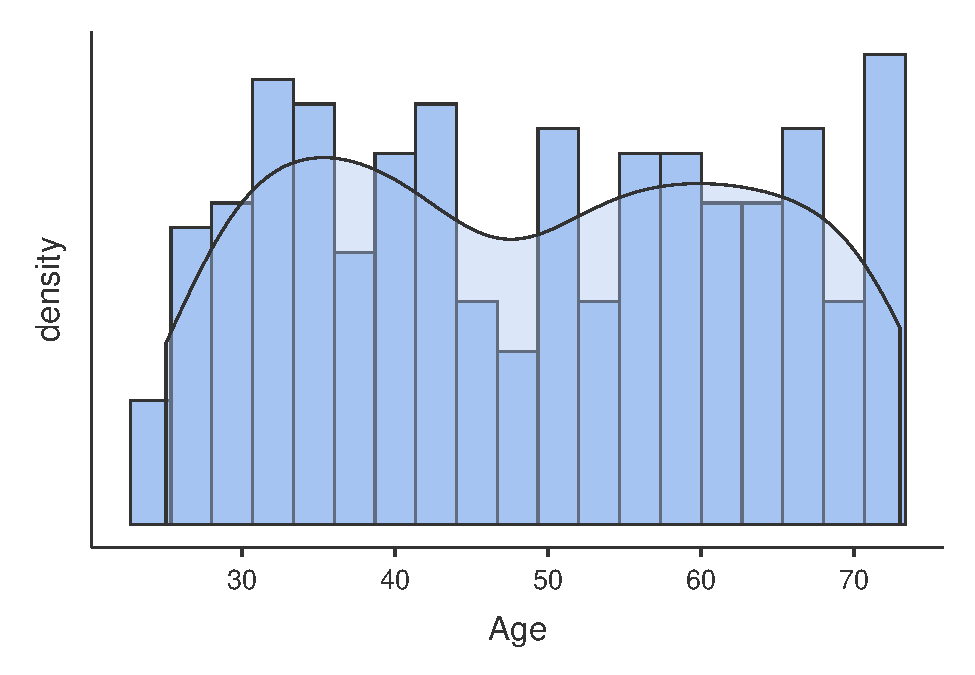
\includegraphics{/Users/serdarbalciold/histopathRprojects/histopathology-template/figs/Descriptive Statistics Age-1.pdf}
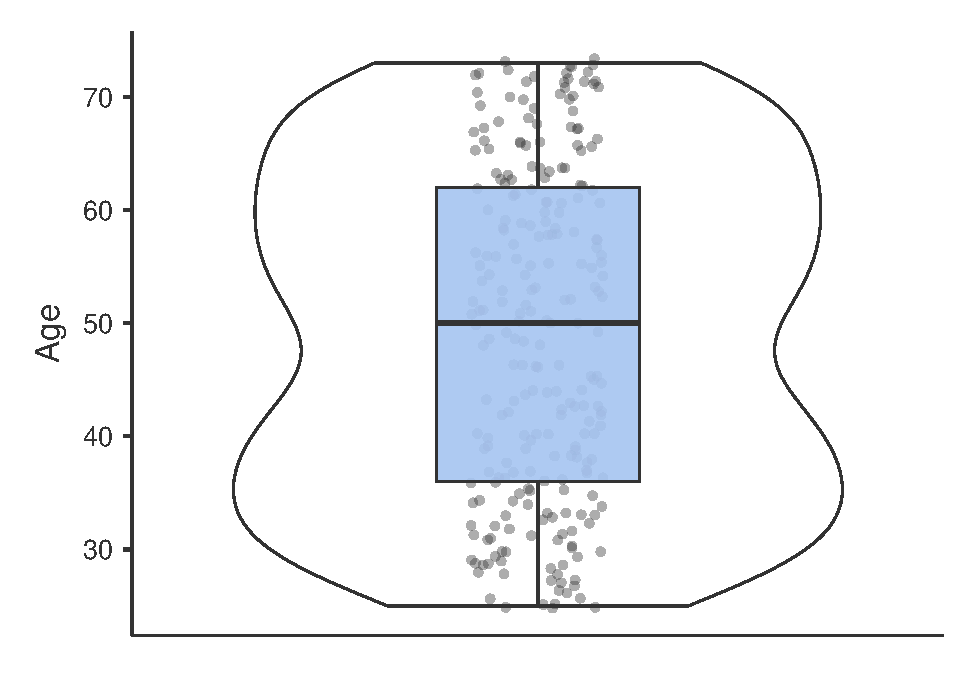
\includegraphics{/Users/serdarbalciold/histopathRprojects/histopathology-template/figs/Descriptive Statistics Age-2.pdf}

\pagebreak

\textbf{Descriptive Statistics AntiX\_intensity}

\begin{Shaded}
\begin{Highlighting}[]
\NormalTok{mydata }\OperatorTok\StringTok{ }\NormalTok{jmv}\OperatorTok{::}\KeywordTok{descriptives}\NormalTok{(}\DataTypeTok{data =}\NormalTok{ ., }\DataTypeTok{vars =} \StringTok{"AntiX_intensity"}\NormalTok{, }\DataTypeTok{hist =} \OtherTok{TRUE}\NormalTok{, }\DataTypeTok{dens =} \OtherTok{TRUE}\NormalTok{, }
    \DataTypeTok{box =} \OtherTok{TRUE}\NormalTok{, }\DataTypeTok{violin =} \OtherTok{TRUE}\NormalTok{, }\DataTypeTok{dot =} \OtherTok{TRUE}\NormalTok{, }\DataTypeTok{mode =} \OtherTok{TRUE}\NormalTok{, }\DataTypeTok{sd =} \OtherTok{TRUE}\NormalTok{, }\DataTypeTok{variance =} \OtherTok{TRUE}\NormalTok{, }
    \DataTypeTok{skew =} \OtherTok{TRUE}\NormalTok{, }\DataTypeTok{kurt =} \OtherTok{TRUE}\NormalTok{, }\DataTypeTok{quart =} \OtherTok{TRUE}\NormalTok{)}
\end{Highlighting}
\end{Shaded}

\begin{verbatim}

 DESCRIPTIVES

 Descriptives                               
 ────────────────────────────────────────── 
                          AntiX_intensity   
 ────────────────────────────────────────── 
   N                                  249   
   Missing                              1   
   Mean                              2.42   
   Median                            3.00   
   Mode                              3.00   
   Standard deviation               0.644   
   Variance                         0.414   
   Minimum                           1.00   
   Maximum                           3.00   
   Skewness                        -0.665   
   Std. error skewness              0.154   
   Kurtosis                        -0.554   
   Std. error kurtosis              0.307   
   25th percentile                   2.00   
   50th percentile                   3.00   
   75th percentile                   3.00   
 ────────────────────────────────────────── 
\end{verbatim}

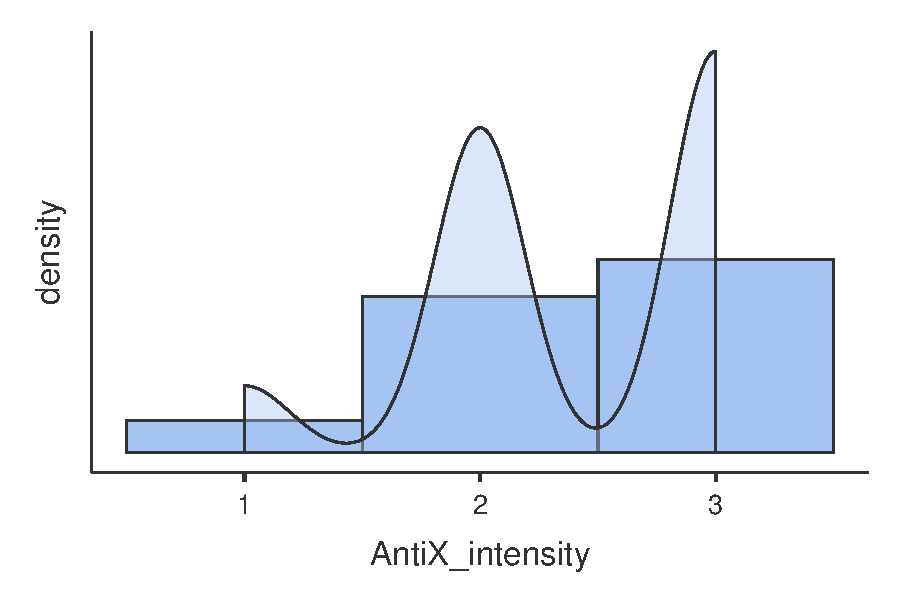
\includegraphics{/Users/serdarbalciold/histopathRprojects/histopathology-template/figs/Descriptive Statistics AntiX_intensity-1.pdf}
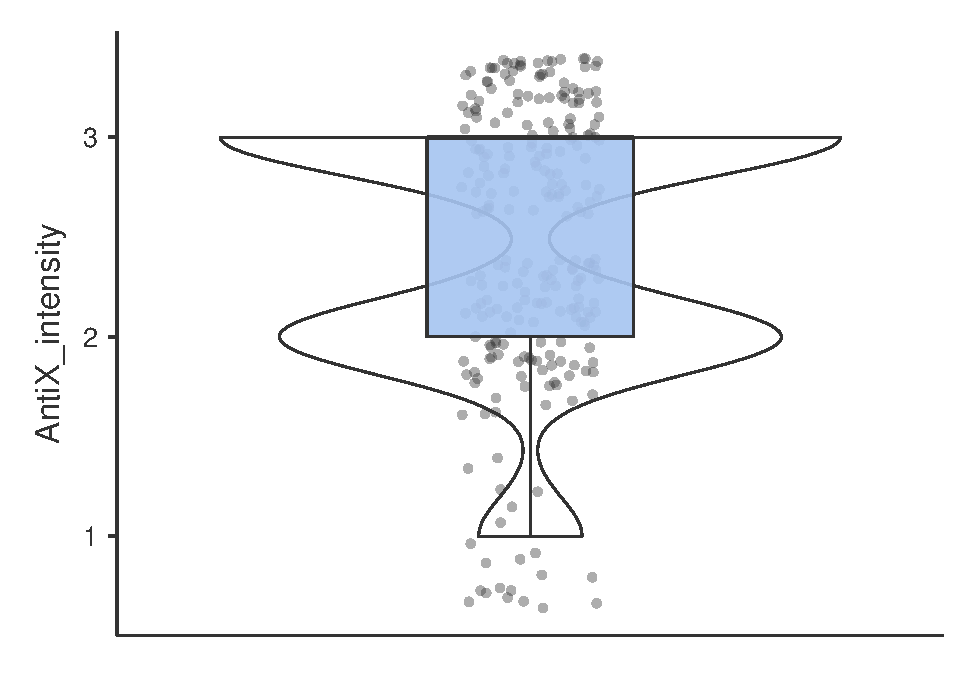
\includegraphics{/Users/serdarbalciold/histopathRprojects/histopathology-template/figs/Descriptive Statistics AntiX_intensity-2.pdf}

\pagebreak

\textbf{Descriptive Statistics AntiY\_intensity}

\begin{Shaded}
\begin{Highlighting}[]
\NormalTok{mydata }\OperatorTok\StringTok{ }\NormalTok{jmv}\OperatorTok{::}\KeywordTok{descriptives}\NormalTok{(}\DataTypeTok{data =}\NormalTok{ ., }\DataTypeTok{vars =} \StringTok{"AntiY_intensity"}\NormalTok{, }\DataTypeTok{hist =} \OtherTok{TRUE}\NormalTok{, }\DataTypeTok{dens =} \OtherTok{TRUE}\NormalTok{, }
    \DataTypeTok{box =} \OtherTok{TRUE}\NormalTok{, }\DataTypeTok{violin =} \OtherTok{TRUE}\NormalTok{, }\DataTypeTok{dot =} \OtherTok{TRUE}\NormalTok{, }\DataTypeTok{mode =} \OtherTok{TRUE}\NormalTok{, }\DataTypeTok{sd =} \OtherTok{TRUE}\NormalTok{, }\DataTypeTok{variance =} \OtherTok{TRUE}\NormalTok{, }
    \DataTypeTok{skew =} \OtherTok{TRUE}\NormalTok{, }\DataTypeTok{kurt =} \OtherTok{TRUE}\NormalTok{, }\DataTypeTok{quart =} \OtherTok{TRUE}\NormalTok{)}
\end{Highlighting}
\end{Shaded}

\begin{verbatim}

 DESCRIPTIVES

 Descriptives                               
 ────────────────────────────────────────── 
                          AntiY_intensity   
 ────────────────────────────────────────── 
   N                                  249   
   Missing                              1   
   Mean                              2.07   
   Median                            2.00   
   Mode                              2.00   
   Standard deviation               0.767   
   Variance                         0.588   
   Minimum                           1.00   
   Maximum                           3.00   
   Skewness                        -0.117   
   Std. error skewness              0.154   
   Kurtosis                         -1.29   
   Std. error kurtosis              0.307   
   25th percentile                   1.00   
   50th percentile                   2.00   
   75th percentile                   3.00   
 ────────────────────────────────────────── 
\end{verbatim}

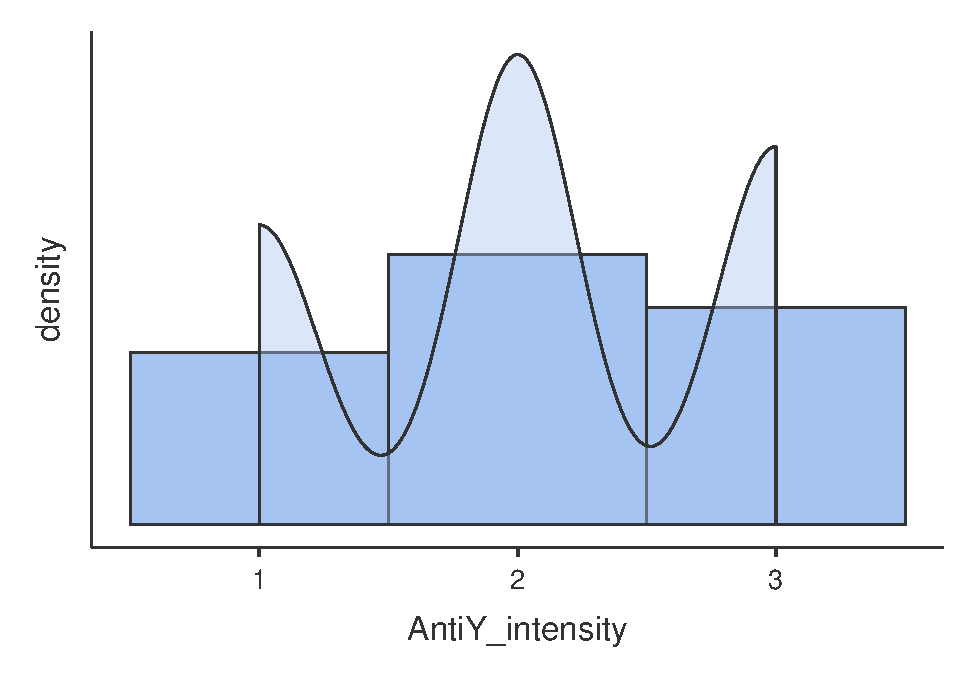
\includegraphics{/Users/serdarbalciold/histopathRprojects/histopathology-template/figs/Descriptive Statistics AntiY_intensity-1.pdf}
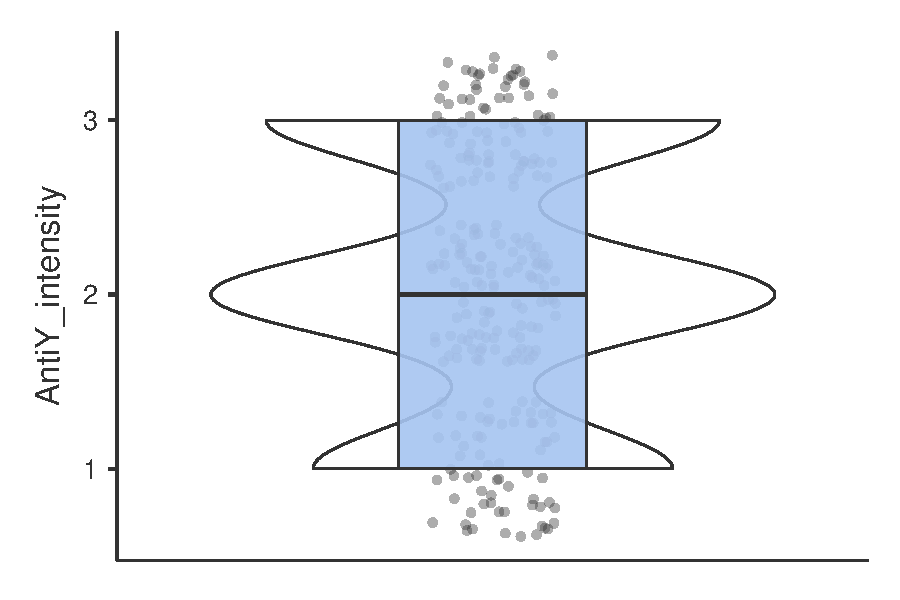
\includegraphics{/Users/serdarbalciold/histopathRprojects/histopathology-template/figs/Descriptive Statistics AntiY_intensity-2.pdf}

\pagebreak

\begin{Shaded}
\begin{Highlighting}[]
\NormalTok{tab <-}\StringTok{ }\NormalTok{tableone}\OperatorTok{::}\KeywordTok{CreateTableOne}\NormalTok{(}\DataTypeTok{data =}\NormalTok{ mydata)}
\CommentTok{# ?print.ContTable}
\NormalTok{tab}\OperatorTok{$}\NormalTok{ContTable}
\end{Highlighting}
\end{Shaded}

\begin{verbatim}
                             
                              Overall      
  n                           250          
  Age (mean (SD))             48.99 (14.44)
  AntiX_intensity (mean (SD))  2.42 (0.64) 
  AntiY_intensity (mean (SD))  2.07 (0.77) 
\end{verbatim}

\begin{Shaded}
\begin{Highlighting}[]
\KeywordTok{print}\NormalTok{(tab}\OperatorTok{$}\NormalTok{ContTable, }\DataTypeTok{nonnormal =} \KeywordTok{c}\NormalTok{(}\StringTok{"Anti-X-intensity"}\NormalTok{))}
\end{Highlighting}
\end{Shaded}

\begin{verbatim}
                             
                              Overall      
  n                           250          
  Age (mean (SD))             48.99 (14.44)
  AntiX_intensity (mean (SD))  2.42 (0.64) 
  AntiY_intensity (mean (SD))  2.07 (0.77) 
\end{verbatim}

\begin{Shaded}
\begin{Highlighting}[]
\NormalTok{mydata }\OperatorTok\StringTok{ }\NormalTok{explore}\OperatorTok{::}\KeywordTok{describe}\NormalTok{(Age)}
\end{Highlighting}
\end{Shaded}

\begin{verbatim}
variable = Age
type     = double
na       = 1 of 250 (0.4%)
unique   = 49
min|max  = 25 | 73
q05|q95  = 27.4 | 71
q25|q75  = 36 | 62
median   = 50
mean     = 48.99197
\end{verbatim}

\begin{Shaded}
\begin{Highlighting}[]
\NormalTok{mydata }\OperatorTok\StringTok{ }\NormalTok{dplyr}\OperatorTok{::}\KeywordTok{select}\NormalTok{(continiousVariables) }\OperatorTok\StringTok{ }\NormalTok{SmartEDA}\OperatorTok{::}\KeywordTok{ExpNumStat}\NormalTok{(}\DataTypeTok{data =}\NormalTok{ ., }
    \DataTypeTok{by =} \StringTok{"A"}\NormalTok{, }\DataTypeTok{gp =} \OtherTok{NULL}\NormalTok{, }\DataTypeTok{Qnt =} \KeywordTok{seq}\NormalTok{(}\DecValTok{0}\NormalTok{, }\DecValTok{1}\NormalTok{, }\FloatTok{0.1}\NormalTok{), }\DataTypeTok{MesofShape =} \DecValTok{2}\NormalTok{, }\DataTypeTok{Outlier =} \OtherTok{TRUE}\NormalTok{, }\DataTypeTok{round =} \DecValTok{2}\NormalTok{)}
\end{Highlighting}
\end{Shaded}

\begin{Shaded}
\begin{Highlighting}[]
\NormalTok{inspectdf}\OperatorTok{::}\KeywordTok{inspect_num}\NormalTok{(mydata, }\DataTypeTok{breaks =} \DecValTok{10}\NormalTok{)}
\end{Highlighting}
\end{Shaded}

\begin{verbatim}
# A tibble: 3 x 10
  col_name        min    q1 median  mean    q3   max     sd pcnt_na hist        
  <chr>         <dbl> <dbl>  <dbl> <dbl> <dbl> <dbl>  <dbl>   <dbl> <named list>
1 Age              25    36     50 49.0     62    73 14.4       0.4 <tibble [12~
2 AntiX_intens~     1     2      3  2.42     3     3  0.644     0.4 <tibble [12~
3 AntiY_intens~     1     1      2  2.07     3     3  0.767     0.4 <tibble [12~
\end{verbatim}

\begin{Shaded}
\begin{Highlighting}[]
\NormalTok{inspectdf}\OperatorTok{::}\KeywordTok{inspect_num}\NormalTok{(mydata)}\OperatorTok{$}\NormalTok{hist}\OperatorTok{$}\NormalTok{Age}
\end{Highlighting}
\end{Shaded}

\begin{verbatim}
# A tibble: 27 x 2
   value        prop
   <chr>       <dbl>
 1 [-Inf, 24) 0     
 2 [24, 26)   0.0201
 3 [26, 28)   0.0321
 4 [28, 30)   0.0482
 5 [30, 32)   0.0442
 6 [32, 34)   0.0482
 7 [34, 36)   0.0402
 8 [36, 38)   0.0482
 9 [38, 40)   0.0442
10 [40, 42)   0.0402
# ... with 17 more rows
\end{verbatim}

\begin{Shaded}
\begin{Highlighting}[]
\NormalTok{inspectdf}\OperatorTok{::}\KeywordTok{inspect_num}\NormalTok{(mydata, }\DataTypeTok{breaks =} \DecValTok{10}\NormalTok{) }\OperatorTok\StringTok{ }\NormalTok{inspectdf}\OperatorTok{::}\KeywordTok{show_plot}\NormalTok{()}
\end{Highlighting}
\end{Shaded}

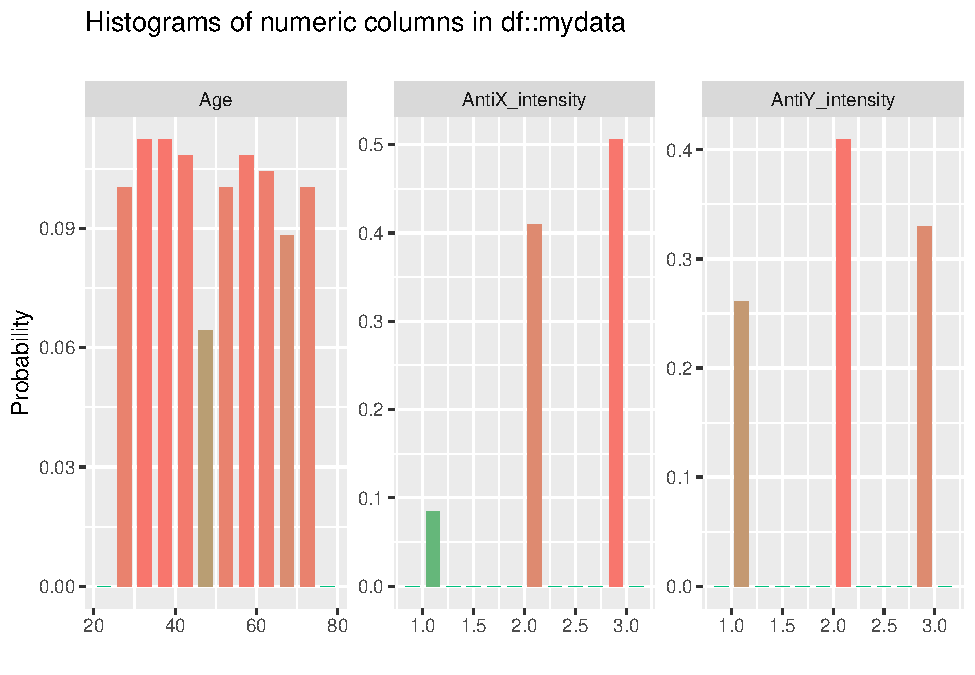
\includegraphics{/Users/serdarbalciold/histopathRprojects/histopathology-template/figs/inspectdf 5-1.pdf}

\hypertarget{split-group-stats-continious}{%
\paragraph{Split-Group Stats
Continious}\label{split-group-stats-continious}}

\begin{Shaded}
\begin{Highlighting}[]
\NormalTok{grouped_descr <-}\StringTok{ }\NormalTok{summarytools}\OperatorTok{::}\KeywordTok{stby}\NormalTok{(}\DataTypeTok{data =}\NormalTok{ mydata, }\DataTypeTok{INDICES =}\NormalTok{ mydata}\OperatorTok{$}\NormalTok{Sex, }\DataTypeTok{FUN =}\NormalTok{ summarytools}\OperatorTok{::}\NormalTok{descr, }
    \DataTypeTok{stats =} \StringTok{"common"}\NormalTok{)}
\CommentTok{# grouped_descr %>% summarytools::tb(order = 2)}
\NormalTok{grouped_descr }\OperatorTok\StringTok{ }\NormalTok{summarytools}\OperatorTok{::}\KeywordTok{tb}\NormalTok{()}
\end{Highlighting}
\end{Shaded}

\hypertarget{grouped-continious}{%
\paragraph{Grouped Continious}\label{grouped-continious}}

\begin{Shaded}
\begin{Highlighting}[]
\NormalTok{summarytools}\OperatorTok{::}\KeywordTok{stby}\NormalTok{(}\DataTypeTok{data =}\NormalTok{ mydata, }\DataTypeTok{INDICES =}\NormalTok{ mydata}\OperatorTok{$}\NormalTok{PreinvasiveComponent, }\DataTypeTok{FUN =}\NormalTok{ summarytools}\OperatorTok{::}\NormalTok{descr, }
    \DataTypeTok{stats =} \KeywordTok{c}\NormalTok{(}\StringTok{"mean"}\NormalTok{, }\StringTok{"sd"}\NormalTok{, }\StringTok{"min"}\NormalTok{, }\StringTok{"med"}\NormalTok{, }\StringTok{"max"}\NormalTok{), }\DataTypeTok{transpose =} \OtherTok{TRUE}\NormalTok{)}
\end{Highlighting}
\end{Shaded}

\begin{Shaded}
\begin{Highlighting}[]
\KeywordTok{with}\NormalTok{(mydata, summarytools}\OperatorTok{::}\KeywordTok{stby}\NormalTok{(Age, PreinvasiveComponent, summarytools}\OperatorTok{::}\NormalTok{descr), }
    \DataTypeTok{stats =} \KeywordTok{c}\NormalTok{(}\StringTok{"mean"}\NormalTok{, }\StringTok{"sd"}\NormalTok{, }\StringTok{"min"}\NormalTok{, }\StringTok{"med"}\NormalTok{, }\StringTok{"max"}\NormalTok{), }\DataTypeTok{transpose =} \OtherTok{TRUE}\NormalTok{)}
\end{Highlighting}
\end{Shaded}

\begin{Shaded}
\begin{Highlighting}[]
\NormalTok{mydata }\OperatorTok\StringTok{ }\KeywordTok{group_by}\NormalTok{(PreinvasiveComponent) }\OperatorTok\StringTok{ }\NormalTok{summarytools}\OperatorTok{::}\KeywordTok{descr}\NormalTok{(}\DataTypeTok{stats =} \StringTok{"fivenum"}\NormalTok{)}
\end{Highlighting}
\end{Shaded}

\begin{Shaded}
\begin{Highlighting}[]
\CommentTok{## Summary statistics by – category}
\NormalTok{SmartEDA}\OperatorTok{::}\KeywordTok{ExpNumStat}\NormalTok{(mydata, }\DataTypeTok{by =} \StringTok{"GA"}\NormalTok{, }\DataTypeTok{gp =} \StringTok{"PreinvasiveComponent"}\NormalTok{, }\DataTypeTok{Qnt =} \KeywordTok{seq}\NormalTok{(}\DecValTok{0}\NormalTok{, }
    \DecValTok{1}\NormalTok{, }\FloatTok{0.1}\NormalTok{), }\DataTypeTok{MesofShape =} \DecValTok{2}\NormalTok{, }\DataTypeTok{Outlier =} \OtherTok{TRUE}\NormalTok{, }\DataTypeTok{round =} \DecValTok{2}\NormalTok{)}
\end{Highlighting}
\end{Shaded}

\begin{verbatim}
  Vname                        Group  TN nNeg nZero nPos NegInf PosInf NA_Value
1   Age     PreinvasiveComponent:All 250    0     0  249      0      0        1
2   Age PreinvasiveComponent:Present  55    0     0   55      0      0        0
3   Age  PreinvasiveComponent:Absent 194    0     0  193      0      0        1
4   Age      PreinvasiveComponent:NA   0    0     0    0      0      0        0
  Per_of_Missing   sum min  max  mean median    SD   CV  IQR Skewness Kurtosis
1           0.40 12199  25   73 48.99     50 14.44 0.29 26.0     0.03    -1.28
2           0.00  2694  25   73 48.98     51 15.22 0.31 26.5    -0.02    -1.29
3           0.52  9449  25   73 48.96     49 14.28 0.29 26.0     0.06    -1.28
4            NaN     0 Inf -Inf   NaN     NA    NA   NA   NA      NaN      NaN
  0%  10%  20%  30%  40% 50%  60% 70% 80%  90% 100% LB.25% UB.75% nOutliers
1 25 29.8 34.0 38.0 43.0  50 54.8  59  64 69.2   73  -3.00 101.00         0
2 25 28.4 32.8 39.2 42.6  51 55.4  59  63 70.0   73  -4.25 101.75         0
3 25 30.2 34.0 38.0 43.0  49 54.0  59  64 69.0   73  -3.00 101.00         0
4 NA   NA   NA   NA   NA  NA   NA  NA  NA   NA   NA     NA     NA         0
\end{verbatim}

\pagebreak

\begin{center}\rule{0.5\linewidth}{0.5pt}\end{center}

\newpage
\begin{landscape}

\hypertarget{cross-tables}{%
\subsection{Cross Tables}\label{cross-tables}}

\textbf{Codes for cross tables}.\footnote{See
  \href{https://github.com/sbalci/histopathology-template/blob/master/childRmd/_12crossTables.Rmd}{\texttt{childRmd/\_12crossTables.Rmd}}
  file for other codes}

\begin{Shaded}
\begin{Highlighting}[]
\KeywordTok{library}\NormalTok{(finalfit)}
\end{Highlighting}
\end{Shaded}

\begin{Shaded}
\begin{Highlighting}[]
\CommentTok{# dependent <- c('dependent1', 'dependent2' )}

\CommentTok{# explanatory <- c('explanatory1', 'explanatory2' )}

\NormalTok{dependent <-}\StringTok{ "PreinvasiveComponent"}

\NormalTok{explanatory <-}\StringTok{ }\KeywordTok{c}\NormalTok{(}\StringTok{"Sex"}\NormalTok{, }\StringTok{"Age"}\NormalTok{, }\StringTok{"Grade"}\NormalTok{, }\StringTok{"TStage"}\NormalTok{)}
\end{Highlighting}
\end{Shaded}

Change \texttt{column\ =\ TRUE} argument to get row or column
percentages.

\begin{Shaded}
\begin{Highlighting}[]
\KeywordTok{source}\NormalTok{(here}\OperatorTok{::}\KeywordTok{here}\NormalTok{(}\StringTok{"R"}\NormalTok{, }\StringTok{"gc_table_cross.R"}\NormalTok{))}
\end{Highlighting}
\end{Shaded}

\textbf{Cross Table PreinvasiveComponent}

\begin{Shaded}
\begin{Highlighting}[]
\NormalTok{mydata }\OperatorTok
\StringTok{    }\KeywordTok{summary_factorlist}\NormalTok{(}\DataTypeTok{dependent =} \StringTok{'PreinvasiveComponent'}\NormalTok{, }
                       \DataTypeTok{explanatory =}\NormalTok{ explanatory,}
                       \CommentTok{# column = TRUE,}
                       \DataTypeTok{total_col =} \OtherTok{TRUE}\NormalTok{,}
                       \DataTypeTok{p =} \OtherTok{TRUE}\NormalTok{,}
                       \DataTypeTok{add_dependent_label =} \OtherTok{TRUE}\NormalTok{,}
                       \DataTypeTok{na_include=}\OtherTok{FALSE}
                       \CommentTok{# catTest = catTestfisher}
\NormalTok{                       ) ->}\StringTok{ }\NormalTok{table}

\NormalTok{knitr}\OperatorTok{::}\KeywordTok{kable}\NormalTok{(table, }\DataTypeTok{row.names =} \OtherTok{FALSE}\NormalTok{, }\DataTypeTok{align =} \KeywordTok{c}\NormalTok{(}\StringTok{'l'}\NormalTok{, }\StringTok{'l'}\NormalTok{, }\StringTok{'r'}\NormalTok{, }\StringTok{'r'}\NormalTok{, }\StringTok{'r'}\NormalTok{))}
\end{Highlighting}
\end{Shaded}

\begin{longtable}[]{@{}llrrrl@{}}
\toprule
Dependent: PreinvasiveComponent & & Absent & Present & Total &
p\tabularnewline
\midrule
\endhead
Sex & Female & 84 (43.5) & 31 (56.4) & 115 (46.4) & 0.092\tabularnewline
& Male & 109 (56.5) & 24 (43.6) & 133 (53.6) &\tabularnewline
Age & Mean (SD) & 49.0 (14.3) & 49.0 (15.2) & 49.0 (14.4) &
0.978\tabularnewline
Grade & 1 & 49 (25.3) & 11 (20.4) & 60 (24.2) & 0.263\tabularnewline
& 2 & 65 (33.5) & 14 (25.9) & 79 (31.9) &\tabularnewline
& 3 & 80 (41.2) & 29 (53.7) & 109 (44.0) &\tabularnewline
TStage & 1 & 17 (8.8) & 4 (7.3) & 21 (8.5) & 0.014\tabularnewline
& 2 & 44 (22.8) & 13 (23.6) & 57 (23.0) &\tabularnewline
& 3 & 33 (17.1) & 20 (36.4) & 53 (21.4) &\tabularnewline
& 4 & 99 (51.3) & 18 (32.7) & 117 (47.2) &\tabularnewline
\bottomrule
\end{longtable}

\pagebreak

\pagebreak

\pagebreak

\pagebreak

\pagebreak

\begin{Shaded}
\begin{Highlighting}[]
\KeywordTok{library}\NormalTok{(DT)}
\KeywordTok{datatable}\NormalTok{(mtcars, }\DataTypeTok{rownames =} \OtherTok{FALSE}\NormalTok{, }\DataTypeTok{filter=}\StringTok{"top"}\NormalTok{, }\DataTypeTok{options =} \KeywordTok{list}\NormalTok{(}\DataTypeTok{pageLength =} \DecValTok{5}\NormalTok{, }\DataTypeTok{scrollX=}\NormalTok{T) )}
\end{Highlighting}
\end{Shaded}

\hypertarget{chi-square-posthoc-pairwise}{%
\subsubsection{chi-square posthoc
pairwise}\label{chi-square-posthoc-pairwise}}

\hypertarget{rmngb}{%
\paragraph{rmngb}\label{rmngb}}

\hypertarget{rvaidememoire}{%
\paragraph{RVAideMemoire}\label{rvaidememoire}}

\newpage
\begin{landscape}

\end{landscape}

\end{landscape}

\hypertarget{plots}{%
\section{Plots}\label{plots}}

\textbf{Codes for generating Plots}.\footnote{See
  \href{https://github.com/sbalci/histopathology-template/blob/master/childRmd/_13plots.Rmd}{\texttt{childRmd/\_13plots.Rmd}}
  file for other codes}

\hypertarget{categorical-variables-1}{%
\subsection{Categorical Variables}\label{categorical-variables-1}}

\hypertarget{plots-1}{%
\section{Plots}\label{plots-1}}

\hypertarget{continious-variables-1}{%
\subsection{Continious Variables}\label{continious-variables-1}}

\hypertarget{interactive}{%
\section{Interactive graphics}\label{interactive}}

\begin{center}\rule{0.5\linewidth}{0.5pt}\end{center}

R allows to build any type of
\href{https://www.r-graph-gallery.com/interactive-charts/}{interactive
graphic}. My favourite library is
\href{https://www.r-graph-gallery.com/get-the-best-from-ggplotly/}{plotly}
that will turn any of your ggplot2 graphic interactive in one
supplementary line of code. Try to hover points, to select a zone, to
click on the legend.

\begin{Shaded}
\begin{Highlighting}[]
\KeywordTok{library}\NormalTok{(ggplot2)}
\KeywordTok{library}\NormalTok{(plotly)}
\KeywordTok{library}\NormalTok{(gapminder)}

\NormalTok{p <-}\StringTok{ }\NormalTok{gapminder }\OperatorTok\StringTok{ }\KeywordTok{filter}\NormalTok{(year }\OperatorTok{==}\StringTok{ }\DecValTok{1977}\NormalTok{) }\OperatorTok\StringTok{ }\KeywordTok{ggplot}\NormalTok{(}\KeywordTok{aes}\NormalTok{(gdpPercap, lifeExp, }\DataTypeTok{size =}\NormalTok{ pop, }
    \DataTypeTok{color =}\NormalTok{ continent)) }\OperatorTok{+}\StringTok{ }\KeywordTok{geom_point}\NormalTok{() }\OperatorTok{+}\StringTok{ }\KeywordTok{scale_x_log10}\NormalTok{() }\OperatorTok{+}\StringTok{ }\KeywordTok{theme_bw}\NormalTok{()}

\KeywordTok{ggplotly}\NormalTok{(p)}
\end{Highlighting}
\end{Shaded}

\textbf{Codes for generating paired tests}.\footnote{See
  \href{https://github.com/sbalci/histopathology-template/blob/master/childRmd/_14pairedTests.Rmd}{\texttt{childRmd/\_14pairedTests.Rmd}}
  file for other codes}

\textbf{Codes for generating hypothesis tests}.\footnote{See
  \href{https://github.com/sbalci/histopathology-template/blob/master/childRmd/_15hypothesisTests.Rmd}{\texttt{childRmd/\_15hypothesisTests.Rmd}}
  file for other codes}

\hypertarget{hypothesis-tests}{%
\section{Hypothesis Tests}\label{hypothesis-tests}}

\hypertarget{tests-of-normality}{%
\subsection{Tests of Normality}\label{tests-of-normality}}

\hypertarget{categorical}{%
\subsection{Categorical}\label{categorical}}

\hypertarget{chi-square-cramer-association-predictive-power}{%
\subsubsection{Chi-Square Cramer Association Predictive
Power}\label{chi-square-cramer-association-predictive-power}}

\hypertarget{continious}{%
\subsection{Continious}\label{continious}}

\url{https://stat.ethz.ch/R-manual/R-devel/library/stats/html/t.test.html}

t.test(mtcars\(mpg ~ mtcars\)am) \%\textgreater\% report::report()

report(t.test(iris\(Sepal.Length, iris\)Petal.Length))

\hypertarget{odds}{%
\subsection{Odds}\label{odds}}

\hypertarget{frequently-used-statistical-tests-by-pathologists}{%
\section{Frequently Used Statistical Tests By
Pathologists}\label{frequently-used-statistical-tests-by-pathologists}}

Frequently Used Statistical Tests\footnote{Statistical Literacy Among
  Academic Pathologists: A Survey Study to Gauge Knowledge of Frequently
  Used Statistical Tests Among Trainees and Faculty. Archives of
  Pathology \& Laboratory Medicine: February 2017, Vol. 141, No.~2,
  pp.~279-287. \url{https://doi.org/10.5858/arpa.2016-0200-OA}} by
(Schmidt et al. 2017)

\begin{itemize}
\tightlist
\item
  Student t test
\item
  Regression/ANOVA
\item
  Chi-square test
\item
  Mann-Whitney test (rank sum)
\item
  Fisher exact test
\item
  Survival analysis

  \begin{itemize}
  \tightlist
  \item
    Kaplan-Meier/log-rank
  \item
    Cox regression
  \end{itemize}
\item
  Multiple comparison adjustment

  \begin{itemize}
  \tightlist
  \item
    Tukey
  \item
    Bonferroni
  \item
    Newman-Keuls
  \end{itemize}
\item
  Kappa Statistic
\item
  ROC analysis
\item
  Logistic regression
\item
  Spearman rank correlation
\item
  Kruskal-Wallis test
\item
  Pearson correlation statistic
\item
  Normality test
\item
  McNemar test
\end{itemize}

\hypertarget{consider-adding}{%
\section{Consider Adding:}\label{consider-adding}}

\begin{itemize}
\tightlist
\item
  \url{https://cran.r-project.org/web/packages/sm/sm.pdf}
\item
  \url{https://cran.r-project.org/web/packages/Rfit/Rfit.pdf}
\end{itemize}

\newpage
\begin{landscape}

\textbf{Codes for ROC}.\footnote{See
  \href{https://github.com/sbalci/histopathology-template/blob/master/childRmd/_16ROC.Rmd}{\texttt{childRmd/\_16ROC.Rmd}}
  file for other codes}

\hypertarget{roc}{%
\section{ROC}\label{roc}}

\textbf{Codes for Decision Tree}.\footnote{See
  \href{https://github.com/sbalci/histopathology-template/blob/master/childRmd/_17decisionTree.Rmd}{\texttt{childRmd/\_17decisionTree.Rmd}}}

\hypertarget{decision-tree}{%
\section{Decision Tree}\label{decision-tree}}

\textbf{Explore}

\begin{Shaded}
\begin{Highlighting}[]
\NormalTok{explore}\OperatorTok{::}\KeywordTok{explore}\NormalTok{(mydata)}
\end{Highlighting}
\end{Shaded}

\hypertarget{survival-analysis}{%
\subsection{Survival Analysis}\label{survival-analysis}}

\textbf{Codes for Survival Analysis}\footnote{See
  \href{https://github.com/sbalci/histopathology-template/blob/master/childRmd/_18survival.Rmd}{\texttt{childRmd/\_18survival.Rmd}}
  file for other codes, and
  \href{https://github.com/sbalci/histopathology-template/blob/master/childRmd/_19shinySurvival.Rmd}{\texttt{childRmd/\_19shinySurvival.Rmd}}
  for \texttt{shiny} application}

\begin{itemize}
\tightlist
\item
  Survival analysis with strata, clusters, frailties and competing risks
  in in Finalfit
\end{itemize}

\url{https://www.datasurg.net/2019/09/12/survival-analysis-with-strata-clusters-frailties-and-competing-risks-in-in-finalfit/}

\begin{itemize}
\tightlist
\item
  Intracranial WHO grade I meningioma: a competing risk analysis of
  progression and disease-specific survival
\end{itemize}

\url{https://link.springer.com/article/10.1007/s00701-019-04096-9}

\textbf{Calculate survival time}

\begin{Shaded}
\begin{Highlighting}[]
\NormalTok{mydata}\OperatorTok{$}\NormalTok{int <-}\StringTok{ }\NormalTok{lubridate}\OperatorTok{::}\KeywordTok{interval}\NormalTok{(lubridate}\OperatorTok{::}\KeywordTok{ymd}\NormalTok{(mydata}\OperatorTok{$}\NormalTok{SurgeryDate), lubridate}\OperatorTok{::}\KeywordTok{ymd}\NormalTok{(mydata}\OperatorTok{$}\NormalTok{LastFollowUpDate))}
\NormalTok{mydata}\OperatorTok{$}\NormalTok{OverallTime <-}\StringTok{ }\NormalTok{lubridate}\OperatorTok{::}\KeywordTok{time_length}\NormalTok{(mydata}\OperatorTok{$}\NormalTok{int, }\StringTok{"month"}\NormalTok{)}
\NormalTok{mydata}\OperatorTok{$}\NormalTok{OverallTime <-}\StringTok{ }\KeywordTok{round}\NormalTok{(mydata}\OperatorTok{$}\NormalTok{OverallTime, }\DataTypeTok{digits =} \DecValTok{1}\NormalTok{)}
\end{Highlighting}
\end{Shaded}

\textbf{recode death status outcome as numbers for survival analysis}

\begin{Shaded}
\begin{Highlighting}[]
\CommentTok{## Recoding mydata$Death into mydata$Outcome}
\NormalTok{mydata}\OperatorTok{$}\NormalTok{Outcome <-}\StringTok{ }\NormalTok{forcats}\OperatorTok{::}\KeywordTok{fct_recode}\NormalTok{(}\KeywordTok{as.character}\NormalTok{(mydata}\OperatorTok{$}\NormalTok{Death), }\StringTok{`}\DataTypeTok{1}\StringTok{`}\NormalTok{ =}\StringTok{ "TRUE"}\NormalTok{, }\StringTok{`}\DataTypeTok{0}\StringTok{`}\NormalTok{ =}\StringTok{ "FALSE"}\NormalTok{)}
\NormalTok{mydata}\OperatorTok{$}\NormalTok{Outcome <-}\StringTok{ }\KeywordTok{as.numeric}\NormalTok{(}\KeywordTok{as.character}\NormalTok{(mydata}\OperatorTok{$}\NormalTok{Outcome))}
\end{Highlighting}
\end{Shaded}

\textbf{it is always a good practice to double-check after
recoding}\footnote{\href{https://www.datasurg.net/2019/10/15/jama-retraction-after-miscoding-new-finalfit-function-to-check-recoding/}{JAMA
  retraction after miscoding -- new Finalfit function to check recoding}}

\begin{Shaded}
\begin{Highlighting}[]
\KeywordTok{table}\NormalTok{(mydata}\OperatorTok{$}\NormalTok{Death, mydata}\OperatorTok{$}\NormalTok{Outcome)}
\end{Highlighting}
\end{Shaded}

\begin{verbatim}
       
          0   1
  FALSE  69   0
  TRUE    0 180
\end{verbatim}

\hypertarget{kaplan-meier}{%
\subsubsection{Kaplan-Meier}\label{kaplan-meier}}

\begin{Shaded}
\begin{Highlighting}[]
\KeywordTok{library}\NormalTok{(survival)}
\CommentTok{# data(lung) km <- with(lung, Surv(time, status))}
\NormalTok{km <-}\StringTok{ }\KeywordTok{with}\NormalTok{(mydata, }\KeywordTok{Surv}\NormalTok{(OverallTime, Outcome))}
\KeywordTok{head}\NormalTok{(km, }\DecValTok{80}\NormalTok{)}
\end{Highlighting}
\end{Shaded}

\begin{verbatim}
 [1]  9.4  11.1   7.3   7.2+  6.3   9.3   9.3   9.2   3.4  11.3   7.5  10.2+
[13]  4.1  10.1   7.3   9.0+  5.1   5.2+  9.3  10.8   3.6   4.1+  5.1   6.2 
[25]  8.9   8.0  11.2  10.5   8.2   7.5+  6.9   5.1+  7.6+  3.6+ 10.3   5.8 
[37]  4.0   3.9    NA   8.4  10.0  11.6   7.6+  8.4   6.7   9.0+  7.4  11.2 
[49]  6.0   9.1+  8.6  10.2   9.2   9.8   7.3  11.1  10.6   4.4+  9.9   6.2+
[61]  6.7   6.7+  8.3   6.5   3.2+  8.1+ 11.0  10.3+  6.3  10.8   3.7   7.1+
[73]  4.2   4.6   9.1   4.4   8.5   8.8+  7.3+ 10.8+
\end{verbatim}

\begin{Shaded}
\begin{Highlighting}[]
\KeywordTok{plot}\NormalTok{(km)}
\end{Highlighting}
\end{Shaded}

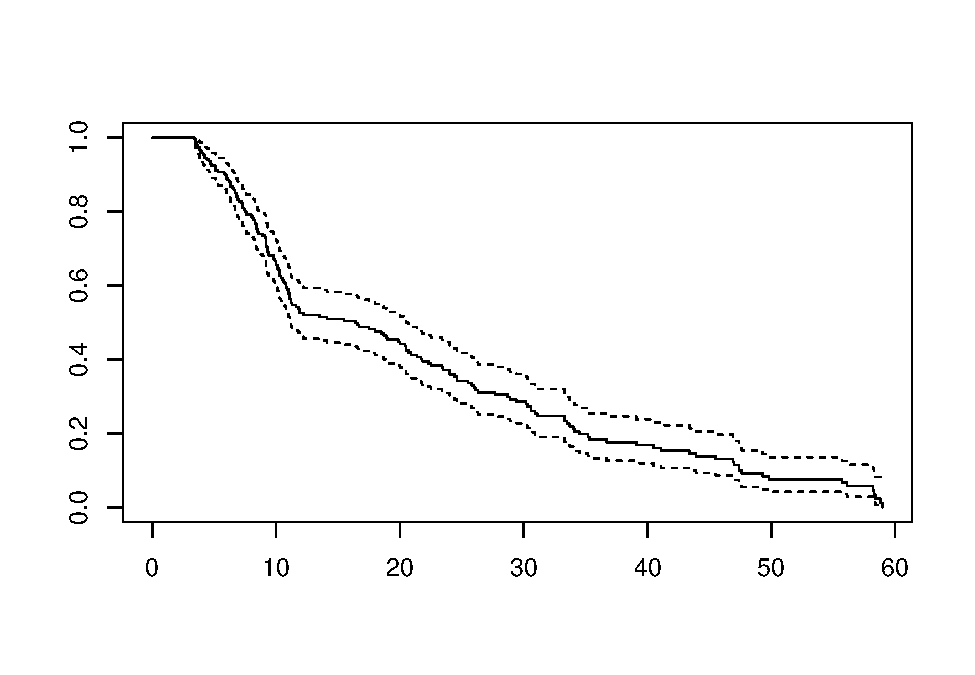
\includegraphics{/Users/serdarbalciold/histopathRprojects/histopathology-template/figs/km-1.pdf}

\textbf{Kaplan-Meier Plot Log-Rank Test}

\begin{Shaded}
\begin{Highlighting}[]
\CommentTok{# Drawing Survival Curves Using ggplot2}
\CommentTok{# https://rpkgs.datanovia.com/survminer/reference/ggsurvplot.html}
\NormalTok{dependentKM <-}\StringTok{ "Surv(OverallTime, Outcome)"}
\NormalTok{explanatoryKM <-}\StringTok{ "LVI"}

\NormalTok{mydata }\OperatorTok
\StringTok{  }\NormalTok{finalfit}\OperatorTok{::}\KeywordTok{surv_plot}\NormalTok{(}\DataTypeTok{.data =}\NormalTok{ .,}
                      \DataTypeTok{dependent =}\NormalTok{ dependentKM,}
                      \DataTypeTok{explanatory =}\NormalTok{ explanatoryKM,}
                      \DataTypeTok{xlab=}\StringTok{'Time (months)'}\NormalTok{,}
                      \DataTypeTok{pval=}\OtherTok{TRUE}\NormalTok{,}
                      \DataTypeTok{legend =} \StringTok{'none'}\NormalTok{,}
                      \DataTypeTok{break.time.by =} \DecValTok{12}\NormalTok{,}
                      \DataTypeTok{xlim =} \KeywordTok{c}\NormalTok{(}\DecValTok{0}\NormalTok{,}\DecValTok{60}\NormalTok{)}
                      \CommentTok{# legend.labs = c('a','b')}
\NormalTok{                      )}
\end{Highlighting}
\end{Shaded}

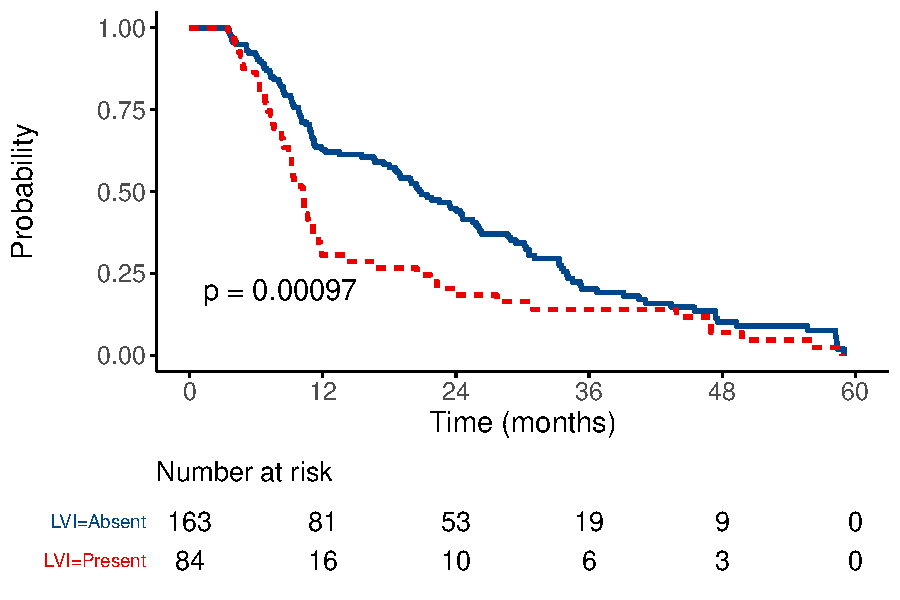
\includegraphics{/Users/serdarbalciold/histopathRprojects/histopathology-template/figs/Kaplan-Meier Plot Log-Rank Test-1.pdf}

\begin{Shaded}
\begin{Highlighting}[]
\CommentTok{# Drawing Survival Curves Using ggplot2}
\CommentTok{# https://rpkgs.datanovia.com/survminer/reference/ggsurvplot.html}

\NormalTok{mydata }\OperatorTok
\StringTok{  }\NormalTok{finalfit}\OperatorTok{::}\KeywordTok{surv_plot}\NormalTok{(}\DataTypeTok{.data =}\NormalTok{ .,}
                      \DataTypeTok{dependent =} \StringTok{"Surv(OverallTime, Outcome)"}\NormalTok{,}
                      \DataTypeTok{explanatory =} \StringTok{"LVI"}\NormalTok{,}
                      \DataTypeTok{xlab=}\StringTok{'Time (months)'}\NormalTok{,}
                      \DataTypeTok{pval=}\OtherTok{TRUE}\NormalTok{,}
                      \DataTypeTok{legend =} \StringTok{'none'}\NormalTok{,}
                      \DataTypeTok{break.time.by =} \DecValTok{12}\NormalTok{,}
                      \DataTypeTok{xlim =} \KeywordTok{c}\NormalTok{(}\DecValTok{0}\NormalTok{,}\DecValTok{60}\NormalTok{)}
                      \CommentTok{# legend.labs = c('a','b')}
\NormalTok{                      )}
\end{Highlighting}
\end{Shaded}

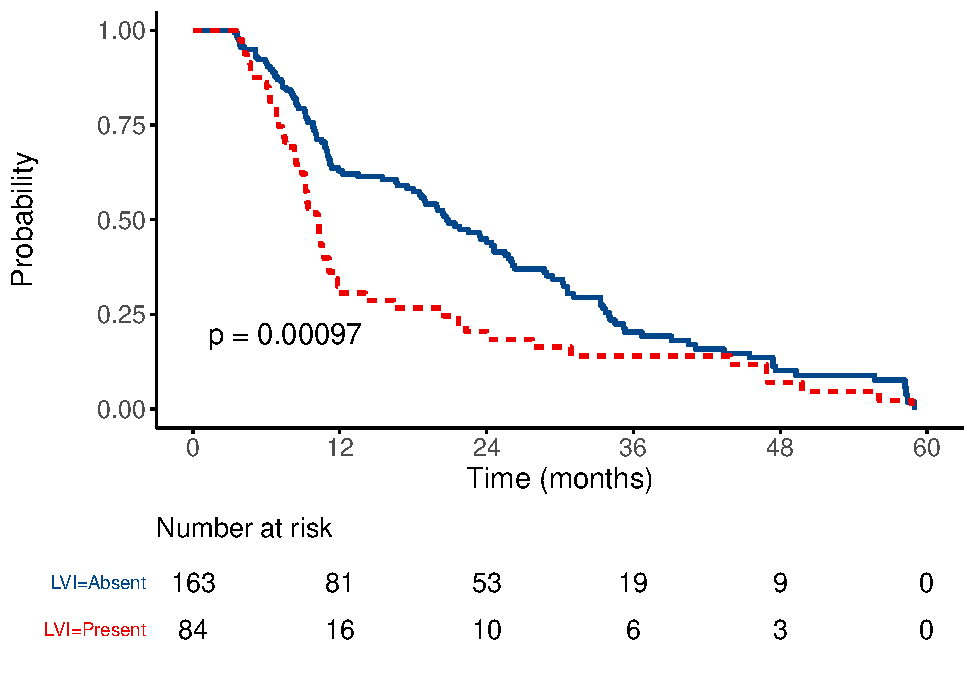
\includegraphics{/Users/serdarbalciold/histopathRprojects/histopathology-template/figs/Kaplan-Meier Plot Log-Rank Test 2-1.pdf}

\hypertarget{univariate-cox-regression}{%
\subsubsection{Univariate
Cox-Regression}\label{univariate-cox-regression}}

\begin{Shaded}
\begin{Highlighting}[]
\KeywordTok{library}\NormalTok{(finalfit)}
\KeywordTok{library}\NormalTok{(survival)}
\NormalTok{explanatoryUni <-}\StringTok{ "LVI"}
\NormalTok{dependentUni <-}\StringTok{ "Surv(OverallTime, Outcome)"}

\NormalTok{tUni <-}\StringTok{ }\NormalTok{mydata }\OperatorTok\StringTok{ }\NormalTok{finalfit}\OperatorTok{::}\KeywordTok{finalfit}\NormalTok{(dependentUni, explanatoryUni)}

\NormalTok{knitr}\OperatorTok{::}\KeywordTok{kable}\NormalTok{(tUni, }\DataTypeTok{row.names =} \OtherTok{FALSE}\NormalTok{, }\DataTypeTok{align =} \KeywordTok{c}\NormalTok{(}\StringTok{"l"}\NormalTok{, }\StringTok{"l"}\NormalTok{, }\StringTok{"r"}\NormalTok{, }\StringTok{"r"}\NormalTok{, }\StringTok{"r"}\NormalTok{, }\StringTok{"r"}\NormalTok{))}
\end{Highlighting}
\end{Shaded}

\begin{longtable}[]{@{}llrrr@{}}
\toprule
Dependent: Surv(OverallTime, Outcome) & & all & HR (univariable) & HR
(multivariable)\tabularnewline
\midrule
\endhead
LVI & Absent & 166 (100.0) & - & -\tabularnewline
& Present & 84 (100.0) & 1.69 (1.23-2.31, p=0.001) & 1.69 (1.23-2.31,
p=0.001)\tabularnewline
\bottomrule
\end{longtable}

\begin{Shaded}
\begin{Highlighting}[]
\NormalTok{tUni_df <-}\StringTok{ }\NormalTok{tibble}\OperatorTok{::}\KeywordTok{as_tibble}\NormalTok{(tUni, }\DataTypeTok{.name_repair =} \StringTok{"minimal"}\NormalTok{) }\OperatorTok\StringTok{ }\NormalTok{janitor}\OperatorTok{::}\KeywordTok{clean_names}\NormalTok{()}

\NormalTok{tUni_df_descr <-}\StringTok{ }\KeywordTok{paste0}\NormalTok{(}\StringTok{"When "}\NormalTok{, tUni_df}\OperatorTok{$}\NormalTok{dependent_surv_overall_time_outcome[}\DecValTok{1}\NormalTok{], }
    \StringTok{" is "}\NormalTok{, tUni_df}\OperatorTok{$}\NormalTok{x[}\DecValTok{2}\NormalTok{], }\StringTok{", there is "}\NormalTok{, tUni_df}\OperatorTok{$}\NormalTok{hr_univariable[}\DecValTok{2}\NormalTok{], }\StringTok{" times risk than "}\NormalTok{, }
    \StringTok{"when "}\NormalTok{, tUni_df}\OperatorTok{$}\NormalTok{dependent_surv_overall_time_outcome[}\DecValTok{1}\NormalTok{], }\StringTok{" is "}\NormalTok{, tUni_df}\OperatorTok{$}\NormalTok{x[}\DecValTok{1}\NormalTok{], }
    \StringTok{"."}\NormalTok{)}
\end{Highlighting}
\end{Shaded}

When LVI is Present, there is 1.69 (1.23-2.31, p=0.001) times risk than
when LVI is Absent.

\noindent

\colorbox{yellow}{
\parbox{\dimexpr\linewidth-2\fboxsep}{

$ When LVI is Present, there is 1.69 (1.23-2.31, p=0.001) times risk than when LVI is Absent. $

}
}

\hypertarget{kaplan-meier-median-survival}{%
\subsubsection{Kaplan-Meier Median
Survival}\label{kaplan-meier-median-survival}}

\begin{Shaded}
\begin{Highlighting}[]
\NormalTok{km_fit <-}\StringTok{ }\KeywordTok{survfit}\NormalTok{(}\KeywordTok{Surv}\NormalTok{(OverallTime, Outcome) }\OperatorTok{~}\StringTok{ }\NormalTok{LVI, }\DataTypeTok{data =}\NormalTok{ mydata)}
\NormalTok{km_fit}
\end{Highlighting}
\end{Shaded}

\begin{verbatim}
Call: survfit(formula = Surv(OverallTime, Outcome) ~ LVI, data = mydata)

   3 observations deleted due to missingness 
              n events median 0.95LCL 0.95UCL
LVI=Absent  163    116   20.7    18.0    25.8
LVI=Present  84     62   10.2     9.2    11.6
\end{verbatim}

\begin{Shaded}
\begin{Highlighting}[]
\KeywordTok{plot}\NormalTok{(km_fit)}
\end{Highlighting}
\end{Shaded}

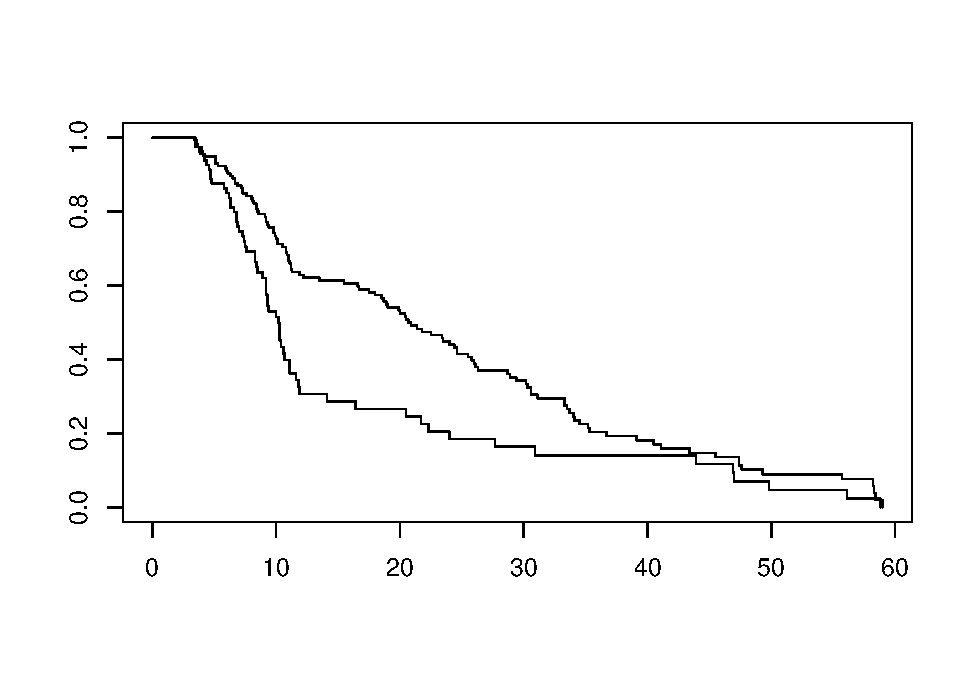
\includegraphics{/Users/serdarbalciold/histopathRprojects/histopathology-template/figs/Median Survivals-1.pdf}

\begin{Shaded}
\begin{Highlighting}[]
\CommentTok{# summary(km_fit)}
\end{Highlighting}
\end{Shaded}

\begin{Shaded}
\begin{Highlighting}[]
\NormalTok{km_fit_median_df <-}\StringTok{ }\KeywordTok{summary}\NormalTok{(km_fit)}
\NormalTok{km_fit_median_df <-}\StringTok{ }\KeywordTok{as.data.frame}\NormalTok{(km_fit_median_df}\OperatorTok{$}\NormalTok{table) }\OperatorTok\StringTok{ }\NormalTok{janitor}\OperatorTok{::}\KeywordTok{clean_names}\NormalTok{() }\OperatorTok\StringTok{ }
\StringTok{    }\NormalTok{tibble}\OperatorTok{::}\KeywordTok{rownames_to_column}\NormalTok{()}
\end{Highlighting}
\end{Shaded}

\begin{Shaded}
\begin{Highlighting}[]
\NormalTok{km_fit_median_definition <-}\StringTok{ }\NormalTok{km_fit_median_df }\OperatorTok\StringTok{ }\NormalTok{dplyr}\OperatorTok{::}\KeywordTok{mutate}\NormalTok{(}\DataTypeTok{description =}\NormalTok{ glue}\OperatorTok{::}\KeywordTok{glue}\NormalTok{(}\StringTok{"When \{rowname\}, median survival is \{median\} [\{x0_95lcl\} - \{x0_95ucl\}, 95% CI] months."}\NormalTok{)) }\OperatorTok\StringTok{ }
\StringTok{    }\NormalTok{dplyr}\OperatorTok{::}\KeywordTok{select}\NormalTok{(description) }\OperatorTok\StringTok{ }\NormalTok{dplyr}\OperatorTok{::}\KeywordTok{pull}\NormalTok{()}
\end{Highlighting}
\end{Shaded}

When LVI=Absent, median survival is 20.7 {[}18 - 25.8, 95\% CI{]}
months., When LVI=Present, median survival is 10.2 {[}9.2 - 11.6, 95\%
CI{]} months.

\noindent

\colorbox{yellow}{
\parbox{\dimexpr\linewidth-2\fboxsep}{

When LVI=Absent, median survival is 20.7 [18 - 25.8, 95% CI] months., When LVI=Present, median survival is 10.2 [9.2 - 11.6, 95% CI] months.

}
}

\hypertarget{yr-survival}{%
\subsubsection{1-3-5-yr survival}\label{yr-survival}}

\begin{Shaded}
\begin{Highlighting}[]
\KeywordTok{summary}\NormalTok{(km_fit, }\DataTypeTok{times =} \KeywordTok{c}\NormalTok{(}\DecValTok{12}\NormalTok{, }\DecValTok{36}\NormalTok{, }\DecValTok{60}\NormalTok{))}
\end{Highlighting}
\end{Shaded}

\begin{verbatim}
Call: survfit(formula = Surv(OverallTime, Outcome) ~ LVI, data = mydata)

3 observations deleted due to missingness 
                LVI=Absent 
 time n.risk n.event survival std.err lower 95% CI upper 95% CI
   12     81      53    0.629  0.0408        0.554        0.714
   36     19      48    0.203  0.0385        0.140        0.295

                LVI=Present 
 time n.risk n.event survival std.err lower 95% CI upper 95% CI
   12     16      48    0.306  0.0586       0.2102        0.446
   36      6       8    0.141  0.0483       0.0716        0.276
\end{verbatim}

\begin{Shaded}
\begin{Highlighting}[]
\NormalTok{km_fit_summary <-}\StringTok{ }\KeywordTok{summary}\NormalTok{(km_fit, }\DataTypeTok{times =} \KeywordTok{c}\NormalTok{(}\DecValTok{12}\NormalTok{, }\DecValTok{36}\NormalTok{, }\DecValTok{60}\NormalTok{))}

\NormalTok{km_fit_df <-}\StringTok{ }\KeywordTok{as.data.frame}\NormalTok{(km_fit_summary[}\KeywordTok{c}\NormalTok{(}\StringTok{"strata"}\NormalTok{, }\StringTok{"time"}\NormalTok{, }\StringTok{"n.risk"}\NormalTok{, }\StringTok{"n.event"}\NormalTok{, }
    \StringTok{"surv"}\NormalTok{, }\StringTok{"std.err"}\NormalTok{, }\StringTok{"lower"}\NormalTok{, }\StringTok{"upper"}\NormalTok{)])}
\end{Highlighting}
\end{Shaded}

\begin{Shaded}
\begin{Highlighting}[]
\NormalTok{km_fit_definition <-}\StringTok{ }\NormalTok{km_fit_df }\OperatorTok\StringTok{ }\NormalTok{dplyr}\OperatorTok{::}\KeywordTok{mutate}\NormalTok{(}\DataTypeTok{description =}\NormalTok{ glue}\OperatorTok{::}\KeywordTok{glue}\NormalTok{(}\StringTok{"When \{strata\}, \{time\} month survival is \{scales::percent(surv)\} [\{scales::percent(lower)\}-\{scales::percent(upper)\}, 95% CI]."}\NormalTok{)) }\OperatorTok\StringTok{ }
\StringTok{    }\NormalTok{dplyr}\OperatorTok{::}\KeywordTok{select}\NormalTok{(description) }\OperatorTok\StringTok{ }\NormalTok{dplyr}\OperatorTok{::}\KeywordTok{pull}\NormalTok{()}
\end{Highlighting}
\end{Shaded}

When LVI=Absent, 12 month survival is 62.9\% {[}55.4\%-71.4\%, 95\%
CI{]}., When LVI=Absent, 36 month survival is 20.3\% {[}14.0\%-29.5\%,
95\% CI{]}., When LVI=Present, 12 month survival is 30.6\%
{[}21.0\%-44.6\%, 95\% CI{]}., When LVI=Present, 36 month survival is
14.1\% {[}7.2\%-27.6\%, 95\% CI{]}.

\noindent

\colorbox{yellow}{
\parbox{\dimexpr\linewidth-2\fboxsep}{

When LVI=Absent, 12 month survival is 62.9% [55.4%-71.4%, 95% CI]., When LVI=Absent, 36 month survival is 20.3% [14.0%-29.5%, 95% CI]., When LVI=Present, 12 month survival is 30.6% [21.0%-44.6%, 95% CI]., When LVI=Present, 36 month survival is 14.1% [7.2%-27.6%, 95% CI].

}
}

\begin{Shaded}
\begin{Highlighting}[]
\KeywordTok{source}\NormalTok{(here}\OperatorTok{::}\KeywordTok{here}\NormalTok{(}\StringTok{"R"}\NormalTok{, }\StringTok{"gc_survival.R"}\NormalTok{))}
\end{Highlighting}
\end{Shaded}

\hypertarget{survival-analysis-lvi}{%
\subsubsection{Survival Analysis LVI}\label{survival-analysis-lvi}}

\textbf{Kaplan-Meier Plot Log-Rank Test}

\begin{Shaded}
\begin{Highlighting}[]
\KeywordTok{library}\NormalTok{(survival)}
\KeywordTok{library}\NormalTok{(survminer)}
\KeywordTok{library}\NormalTok{(finalfit)}

\NormalTok{mydata }\OperatorTok
\StringTok{  }\NormalTok{finalfit}\OperatorTok{::}\KeywordTok{surv_plot}\NormalTok{(}\StringTok{'Surv(OverallTime, Outcome)'}\NormalTok{, }\StringTok{'LVI'}\NormalTok{, }
  \DataTypeTok{xlab=}\StringTok{'Time (months)'}\NormalTok{, }\DataTypeTok{pval=}\OtherTok{TRUE}\NormalTok{, }\DataTypeTok{legend =} \StringTok{'none'}\NormalTok{,}
    \DataTypeTok{break.time.by =} \DecValTok{12}\NormalTok{, }\DataTypeTok{xlim =} \KeywordTok{c}\NormalTok{(}\DecValTok{0}\NormalTok{,}\DecValTok{60}\NormalTok{)}

\CommentTok{# legend.labs = c('a','b')}

\NormalTok{)}
\end{Highlighting}
\end{Shaded}

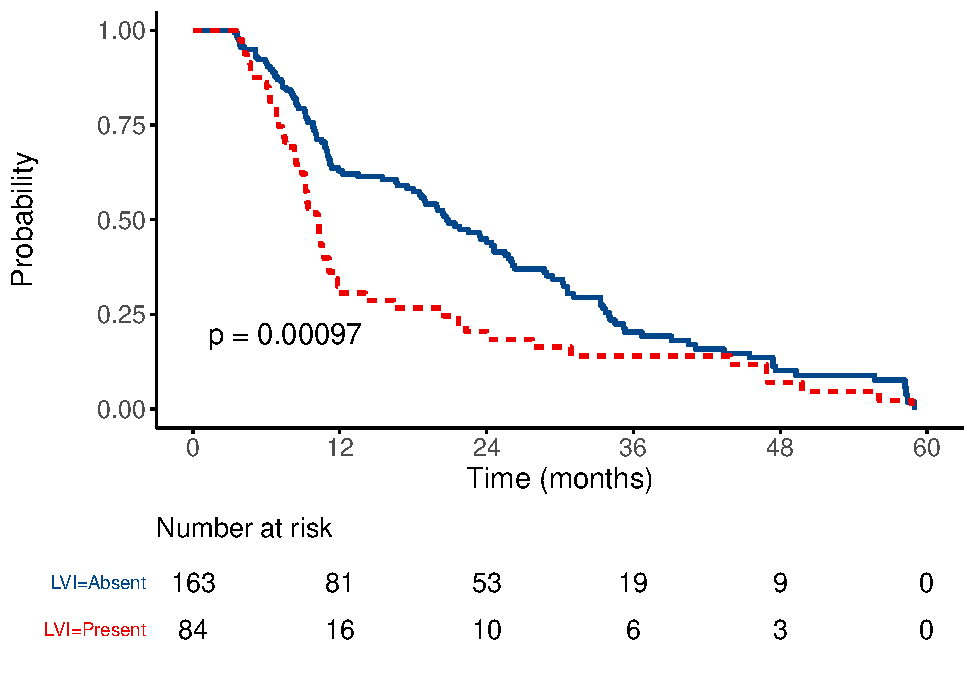
\includegraphics{/Users/serdarbalciold/histopathRprojects/histopathology-template/figs/Kaplan-Meier LVI-1.pdf}

\textbf{Univariate Cox-Regression}

\begin{Shaded}
\begin{Highlighting}[]
\NormalTok{explanatoryUni <-}\StringTok{ "LVI"}
\NormalTok{dependentUni <-}\StringTok{ "Surv(OverallTime, Outcome)"}
\NormalTok{tUni <-}\StringTok{ }\NormalTok{mydata }\OperatorTok\StringTok{ }\KeywordTok{finalfit}\NormalTok{(dependentUni, explanatoryUni, }\DataTypeTok{metrics =} \OtherTok{TRUE}\NormalTok{)}

\NormalTok{knitr}\OperatorTok{::}\KeywordTok{kable}\NormalTok{(tUni, }\DataTypeTok{row.names =} \OtherTok{FALSE}\NormalTok{, }\DataTypeTok{align =} \KeywordTok{c}\NormalTok{(}\StringTok{"l"}\NormalTok{, }\StringTok{"l"}\NormalTok{, }\StringTok{"r"}\NormalTok{, }\StringTok{"r"}\NormalTok{, }\StringTok{"r"}\NormalTok{, }\StringTok{"r"}\NormalTok{))}
\end{Highlighting}
\end{Shaded}

\begin{table}

\centering
\begin{tabular}[t]{l|l|r|r|r}
\hline
Dependent: Surv(OverallTime, Outcome) &   & all & HR (univariable) & HR (multivariable)\\
\hline
LVI & Absent & 166 (100.0) & - & -\\
\hline
 & Present & 84 (100.0) & 1.69 (1.23-2.31, p=0.001) & 1.69 (1.23-2.31, p=0.001)\\
\hline
\end{tabular}
\centering
\begin{tabular}[t]{l}
\hline
x\\
\hline
Number in dataframe = 250, Number in model = 247, Missing = 3, Number of events = 178, Concordance = 0.576 (SE = 0.020), R-squared = 0.040( Max possible = 0.998), Likelihood ratio test = 10.075 (df = 1, p = 0.002)\\
\hline
\end{tabular}
\end{table}

\textbf{Univariate Cox-Regression Summary}

\begin{Shaded}
\begin{Highlighting}[]
\NormalTok{tUni_df <-}\StringTok{ }\NormalTok{tibble}\OperatorTok{::}\KeywordTok{as_tibble}\NormalTok{(tUni, }\DataTypeTok{.name_repair =} \StringTok{"minimal"}\NormalTok{) }\OperatorTok\StringTok{ }\NormalTok{janitor}\OperatorTok{::}\KeywordTok{clean_names}\NormalTok{(}\DataTypeTok{dat =}\NormalTok{ ., }
    \DataTypeTok{case =} \StringTok{"snake"}\NormalTok{)}


\NormalTok{n_level <-}\StringTok{ }\KeywordTok{dim}\NormalTok{(tUni_df)[}\DecValTok{1}\NormalTok{]}

\NormalTok{tUni_df_descr <-}\StringTok{ }\ControlFlowTok{function}\NormalTok{(n) \{}
    \KeywordTok{paste0}\NormalTok{(}\StringTok{"When "}\NormalTok{, tUni_df}\OperatorTok{$}\NormalTok{dependent_surv_overall_time_outcome[}\DecValTok{1}\NormalTok{], }\StringTok{" is "}\NormalTok{, tUni_df}\OperatorTok{$}\NormalTok{x[n }\OperatorTok{+}\StringTok{ }
\StringTok{        }\DecValTok{1}\NormalTok{], }\StringTok{", there is "}\NormalTok{, tUni_df}\OperatorTok{$}\NormalTok{hr_univariable[n }\OperatorTok{+}\StringTok{ }\DecValTok{1}\NormalTok{], }\StringTok{" times risk than "}\NormalTok{, }\StringTok{"when "}\NormalTok{, }
\NormalTok{        tUni_df}\OperatorTok{$}\NormalTok{dependent_surv_overall_time_outcome[}\DecValTok{1}\NormalTok{], }\StringTok{" is "}\NormalTok{, tUni_df}\OperatorTok{$}\NormalTok{x[}\DecValTok{1}\NormalTok{], }\StringTok{"."}\NormalTok{)}
    
\NormalTok{\}}



\NormalTok{results5 <-}\StringTok{ }\NormalTok{purrr}\OperatorTok{::}\KeywordTok{map}\NormalTok{(}\DataTypeTok{.x =} \KeywordTok{c}\NormalTok{(}\DecValTok{2}\OperatorTok{:}\NormalTok{n_level }\OperatorTok{-}\StringTok{ }\DecValTok{1}\NormalTok{), }\DataTypeTok{.f =}\NormalTok{ tUni_df_descr)}

\KeywordTok{print}\NormalTok{(}\KeywordTok{unlist}\NormalTok{(results5))}
\end{Highlighting}
\end{Shaded}

\begin{verbatim}
[1] "When  is c(\"Absent\", \"Present\"), there is  times risk than when  is c(\"LVI\", \"\")."
\end{verbatim}

\pagebreak

\textbf{Median Survival}

\begin{Shaded}
\begin{Highlighting}[]
\NormalTok{km_fit <-}\StringTok{ }\KeywordTok{survfit}\NormalTok{(}\KeywordTok{Surv}\NormalTok{(OverallTime, Outcome) }\OperatorTok{~}\StringTok{ }\NormalTok{LVI, }\DataTypeTok{data =}\NormalTok{ mydata)}
\NormalTok{km_fit}
\end{Highlighting}
\end{Shaded}

\begin{verbatim}
Call: survfit(formula = Surv(OverallTime, Outcome) ~ LVI, data = mydata)

   3 observations deleted due to missingness 
              n events median 0.95LCL 0.95UCL
LVI=Absent  163    116   20.7    18.0    25.8
LVI=Present  84     62   10.2     9.2    11.6
\end{verbatim}

\begin{Shaded}
\begin{Highlighting}[]
\NormalTok{km_fit_median_df <-}\StringTok{ }\KeywordTok{summary}\NormalTok{(km_fit)}
\NormalTok{km_fit_median_df <-}\StringTok{ }\KeywordTok{as.data.frame}\NormalTok{(km_fit_median_df}\OperatorTok{$}\NormalTok{table) }\OperatorTok\StringTok{ }\NormalTok{janitor}\OperatorTok{::}\KeywordTok{clean_names}\NormalTok{(}\DataTypeTok{dat =}\NormalTok{ ., }
    \DataTypeTok{case =} \StringTok{"snake"}\NormalTok{) }\OperatorTok\StringTok{ }\NormalTok{tibble}\OperatorTok{::}\KeywordTok{rownames_to_column}\NormalTok{(}\DataTypeTok{.data =}\NormalTok{ ., }\DataTypeTok{var =} \StringTok{"LVI"}\NormalTok{)}



\NormalTok{km_fit_median_definition <-}\StringTok{ }\NormalTok{km_fit_median_df }\OperatorTok\StringTok{ }\NormalTok{dplyr}\OperatorTok{::}\KeywordTok{mutate}\NormalTok{(}\DataTypeTok{description =}\NormalTok{ glue}\OperatorTok{::}\KeywordTok{glue}\NormalTok{(}\StringTok{"When, LVI, \{LVI\}, median survival is \{median\} [\{x0_95lcl\} - \{x0_95ucl\}, 95% CI] months."}\NormalTok{)) }\OperatorTok\StringTok{ }
\StringTok{    }\NormalTok{dplyr}\OperatorTok{::}\KeywordTok{mutate}\NormalTok{(}\DataTypeTok{description =} \KeywordTok{gsub}\NormalTok{(}\DataTypeTok{pattern =} \StringTok{"thefactor="}\NormalTok{, }\DataTypeTok{replacement =} \StringTok{" is "}\NormalTok{, }
        \DataTypeTok{x =}\NormalTok{ description)) }\OperatorTok\StringTok{ }\NormalTok{dplyr}\OperatorTok{::}\KeywordTok{select}\NormalTok{(description) }\OperatorTok\StringTok{ }\NormalTok{dplyr}\OperatorTok{::}\KeywordTok{pull}\NormalTok{()}

\NormalTok{km_fit_median_definition}
\end{Highlighting}
\end{Shaded}

\begin{verbatim}
When, LVI, LVI=Absent, median survival is 20.7 [18 - 25.8, 95% CI] months.
When, LVI, LVI=Present, median survival is 10.2 [9.2 - 11.6, 95% CI] months.
\end{verbatim}

\textbf{1-3-5-yr survival}

\begin{Shaded}
\begin{Highlighting}[]
\KeywordTok{summary}\NormalTok{(km_fit, }\DataTypeTok{times =} \KeywordTok{c}\NormalTok{(}\DecValTok{12}\NormalTok{, }\DecValTok{36}\NormalTok{, }\DecValTok{60}\NormalTok{))}
\end{Highlighting}
\end{Shaded}

\begin{verbatim}
Call: survfit(formula = Surv(OverallTime, Outcome) ~ LVI, data = mydata)

3 observations deleted due to missingness 
                LVI=Absent 
 time n.risk n.event survival std.err lower 95% CI upper 95% CI
   12     81      53    0.629  0.0408        0.554        0.714
   36     19      48    0.203  0.0385        0.140        0.295

                LVI=Present 
 time n.risk n.event survival std.err lower 95% CI upper 95% CI
   12     16      48    0.306  0.0586       0.2102        0.446
   36      6       8    0.141  0.0483       0.0716        0.276
\end{verbatim}

\begin{Shaded}
\begin{Highlighting}[]
\NormalTok{km_fit_summary <-}\StringTok{ }\KeywordTok{summary}\NormalTok{(km_fit, }\DataTypeTok{times =} \KeywordTok{c}\NormalTok{(}\DecValTok{12}\NormalTok{, }\DecValTok{36}\NormalTok{, }\DecValTok{60}\NormalTok{))}

\NormalTok{km_fit_df <-}\StringTok{ }\KeywordTok{as.data.frame}\NormalTok{(km_fit_summary[}\KeywordTok{c}\NormalTok{(}\StringTok{"strata"}\NormalTok{, }\StringTok{"time"}\NormalTok{, }\StringTok{"n.risk"}\NormalTok{, }\StringTok{"n.event"}\NormalTok{, }
    \StringTok{"surv"}\NormalTok{, }\StringTok{"std.err"}\NormalTok{, }\StringTok{"lower"}\NormalTok{, }\StringTok{"upper"}\NormalTok{)])}

\NormalTok{km_fit_df}
\end{Highlighting}
\end{Shaded}

\begin{verbatim}
       strata time n.risk n.event      surv    std.err     lower     upper
1  LVI=Absent   12     81      53 0.6289603 0.04083915 0.5538010 0.7143200
2  LVI=Absent   36     19      48 0.2032782 0.03847378 0.1402771 0.2945743
3 LVI=Present   12     16      48 0.3060515 0.05864373 0.2102289 0.4455501
4 LVI=Present   36      6       8 0.1405339 0.04832884 0.0716238 0.2757431
\end{verbatim}

\begin{Shaded}
\begin{Highlighting}[]
\NormalTok{km_fit_definition <-}\StringTok{ }\NormalTok{km_fit_df }\OperatorTok\StringTok{ }\NormalTok{dplyr}\OperatorTok{::}\KeywordTok{mutate}\NormalTok{(}\DataTypeTok{description =}\NormalTok{ glue}\OperatorTok{::}\KeywordTok{glue}\NormalTok{(}\StringTok{"When \{strata\}, \{time\} month survival is \{scales::percent(surv)\} [\{scales::percent(lower)\}-\{scales::percent(upper)\}, 95% CI]."}\NormalTok{)) }\OperatorTok\StringTok{ }
\StringTok{    }\NormalTok{dplyr}\OperatorTok{::}\KeywordTok{select}\NormalTok{(description) }\OperatorTok\StringTok{ }\NormalTok{dplyr}\OperatorTok{::}\KeywordTok{pull}\NormalTok{()}

\NormalTok{km_fit_definition}
\end{Highlighting}
\end{Shaded}

\begin{verbatim}
When LVI=Absent, 12 month survival is 62.9% [55.4%-71.4%, 95% CI].
When LVI=Absent, 36 month survival is 20.3% [14.0%-29.5%, 95% CI].
When LVI=Present, 12 month survival is 30.6% [21.0%-44.6%, 95% CI].
When LVI=Present, 36 month survival is 14.1% [7.2%-27.6%, 95% CI].
\end{verbatim}

\pagebreak

\begin{Shaded}
\begin{Highlighting}[]
\KeywordTok{summary}\NormalTok{(km_fit)}\OperatorTok{$}\NormalTok{table}
\end{Highlighting}
\end{Shaded}

\begin{verbatim}
            records n.max n.start events   *rmean *se(rmean) median 0.95LCL
LVI=Absent      163   163     163    116 23.99525   1.447518   20.7    18.0
LVI=Present      84    84      84     62 16.43902   1.977111   10.2     9.2
            0.95UCL
LVI=Absent     25.8
LVI=Present    11.6
\end{verbatim}

\begin{Shaded}
\begin{Highlighting}[]
\NormalTok{km_fit_median_df <-}\StringTok{ }\KeywordTok{summary}\NormalTok{(km_fit)}
\NormalTok{results1html <-}\StringTok{ }\KeywordTok{as.data.frame}\NormalTok{(km_fit_median_df}\OperatorTok{$}\NormalTok{table) }\OperatorTok\StringTok{ }\NormalTok{janitor}\OperatorTok{::}\KeywordTok{clean_names}\NormalTok{(}\DataTypeTok{dat =}\NormalTok{ ., }
    \DataTypeTok{case =} \StringTok{"snake"}\NormalTok{) }\OperatorTok\StringTok{ }\NormalTok{tibble}\OperatorTok{::}\KeywordTok{rownames_to_column}\NormalTok{(}\DataTypeTok{.data =}\NormalTok{ ., }\DataTypeTok{var =} \StringTok{"LVI"}\NormalTok{)}

\NormalTok{results1html[, }\DecValTok{1}\NormalTok{] <-}\StringTok{ }\KeywordTok{gsub}\NormalTok{(}\DataTypeTok{pattern =} \StringTok{"thefactor="}\NormalTok{, }\DataTypeTok{replacement =} \StringTok{""}\NormalTok{, }\DataTypeTok{x =}\NormalTok{ results1html[, }
    \DecValTok{1}\NormalTok{])}

\NormalTok{knitr}\OperatorTok{::}\KeywordTok{kable}\NormalTok{(results1html, }\DataTypeTok{row.names =} \OtherTok{FALSE}\NormalTok{, }\DataTypeTok{align =} \KeywordTok{c}\NormalTok{(}\StringTok{"l"}\NormalTok{, }\KeywordTok{rep}\NormalTok{(}\StringTok{"r"}\NormalTok{, }\DecValTok{9}\NormalTok{)), }\DataTypeTok{format =} \StringTok{"html"}\NormalTok{, }
    \DataTypeTok{digits =} \DecValTok{1}\NormalTok{)}
\end{Highlighting}
\end{Shaded}

LVI

records

n\_max

n\_start

events

rmean

se\_rmean

median

x0\_95lcl

x0\_95ucl

LVI=Absent

163

163

163

116

24.0

1.4

20.7

18.0

25.8

LVI=Present

84

84

84

62

16.4

2.0

10.2

9.2

11.6

\pagebreak

\textbf{Pairwise Comparisons}

\pagebreak

\hypertarget{pairwise-comparison}{%
\subsubsection{Pairwise comparison}\label{pairwise-comparison}}

\begin{Shaded}
\begin{Highlighting}[]
\NormalTok{dependentKM <-}\StringTok{ "Surv(OverallTime, Outcome)"}
\NormalTok{explanatoryKM <-}\StringTok{ "TStage"}

\NormalTok{mydata }\OperatorTok
\StringTok{  }\NormalTok{finalfit}\OperatorTok{::}\KeywordTok{surv_plot}\NormalTok{(}\DataTypeTok{.data =}\NormalTok{ .,}
                      \DataTypeTok{dependent =}\NormalTok{ dependentKM,}
                      \DataTypeTok{explanatory =}\NormalTok{ explanatoryKM,}
                      \DataTypeTok{xlab=}\StringTok{'Time (months)'}\NormalTok{,}
                      \DataTypeTok{pval=}\OtherTok{TRUE}\NormalTok{,}
                      \DataTypeTok{legend =} \StringTok{'none'}\NormalTok{,}
                      \DataTypeTok{break.time.by =} \DecValTok{12}\NormalTok{,}
                      \DataTypeTok{xlim =} \KeywordTok{c}\NormalTok{(}\DecValTok{0}\NormalTok{,}\DecValTok{60}\NormalTok{)}
                      \CommentTok{# legend.labs = c('a','b')}
\NormalTok{                      )}
\end{Highlighting}
\end{Shaded}

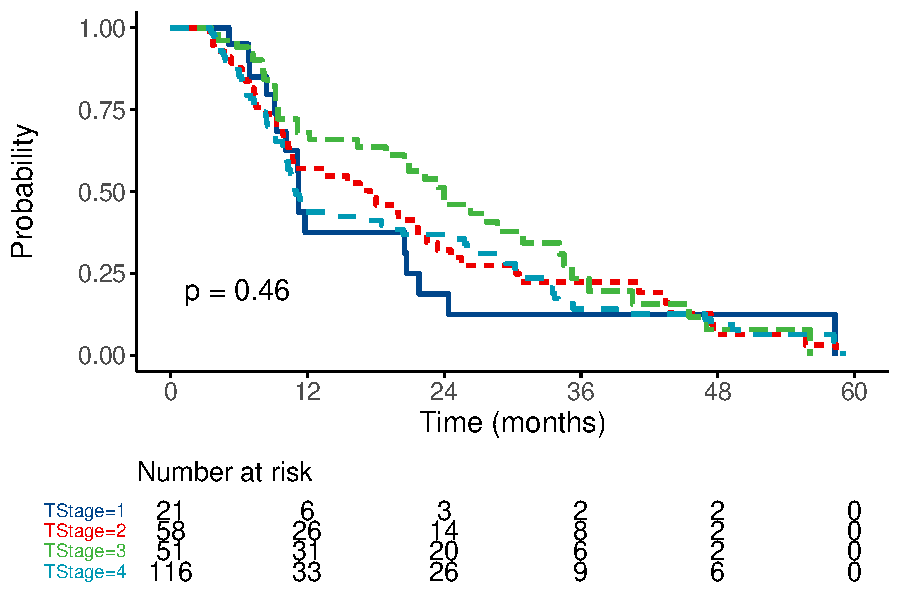
\includegraphics{/Users/serdarbalciold/histopathRprojects/histopathology-template/figs/Kaplan-Meier Plot Log-Rank Test TStage-1.pdf}

\begin{Shaded}
\begin{Highlighting}[]
\NormalTok{km_fit}
\end{Highlighting}
\end{Shaded}

\begin{verbatim}
Call: survfit(formula = Surv(OverallTime, Outcome) ~ LVI, data = mydata)

   3 observations deleted due to missingness 
              n events median 0.95LCL 0.95UCL
LVI=Absent  163    116   20.7    18.0    25.8
LVI=Present  84     62   10.2     9.2    11.6
\end{verbatim}

\begin{Shaded}
\begin{Highlighting}[]
\KeywordTok{print}\NormalTok{(km_fit, }
      \DataTypeTok{scale=}\DecValTok{1}\NormalTok{,}
      \DataTypeTok{digits =} \KeywordTok{max}\NormalTok{(}\KeywordTok{options}\NormalTok{()}\OperatorTok{$}\NormalTok{digits }\OperatorTok{-}\StringTok{ }\DecValTok{4}\NormalTok{,}\DecValTok{3}\NormalTok{),}
      \DataTypeTok{print.rmean=}\KeywordTok{getOption}\NormalTok{(}\StringTok{"survfit.print.rmean"}\NormalTok{),}
      \DataTypeTok{rmean =} \KeywordTok{getOption}\NormalTok{(}\StringTok{'survfit.rmean'}\NormalTok{),}
      \DataTypeTok{print.median=}\KeywordTok{getOption}\NormalTok{(}\StringTok{"survfit.print.median"}\NormalTok{),}
      \DataTypeTok{median =} \KeywordTok{getOption}\NormalTok{(}\StringTok{'survfit.median'}\NormalTok{)}
      
\NormalTok{      )}
\end{Highlighting}
\end{Shaded}

\begin{verbatim}
Call: survfit(formula = Surv(OverallTime, Outcome) ~ LVI, data = mydata)

   3 observations deleted due to missingness 
              n events median 0.95LCL 0.95UCL
LVI=Absent  163    116   20.7    18.0    25.8
LVI=Present  84     62   10.2     9.2    11.6
\end{verbatim}

\hypertarget{multivariate-analysis-survival}{%
\subsubsection{Multivariate Analysis
Survival}\label{multivariate-analysis-survival}}

explanatory = c(``age.factor'', ``sex.factor'', ``obstruct.factor'',
``perfor.factor'') dependent = `mort\_5yr' colon\_s \%\textgreater\%
hr\_plot(dependent, explanatory)

\begin{Shaded}
\begin{Highlighting}[]
\KeywordTok{library}\NormalTok{(survival)}
\KeywordTok{library}\NormalTok{(survminer)}
\KeywordTok{library}\NormalTok{(finalfit)}
\NormalTok{mb_followup }\OperatorTok
\StringTok{  }\NormalTok{finalfit}\OperatorTok{::}\KeywordTok{surv_plot}\NormalTok{(}\StringTok{'Surv(OverallTime, Outcome)'}\NormalTok{, }\StringTok{'Operation'}\NormalTok{, }
  \DataTypeTok{xlab=}\StringTok{'Time (months)'}\NormalTok{, }\DataTypeTok{pval=}\OtherTok{TRUE}\NormalTok{, }\DataTypeTok{legend =} \StringTok{'none'}\NormalTok{,}
  \CommentTok{# pval.coord}
    \DataTypeTok{break.time.by =} \DecValTok{12}\NormalTok{, }\DataTypeTok{xlim =} \KeywordTok{c}\NormalTok{(}\DecValTok{0}\NormalTok{,}\DecValTok{60}\NormalTok{), }\DataTypeTok{ylim =} \KeywordTok{c}\NormalTok{(}\FloatTok{0.8}\NormalTok{, }\DecValTok{1}\NormalTok{)}

\CommentTok{# legend.labs = c('a','b')}

\NormalTok{)}
\end{Highlighting}
\end{Shaded}

\textbf{Univariate Cox-Regression}

\begin{Shaded}
\begin{Highlighting}[]
\NormalTok{explanatoryUni <-}\StringTok{ "Operation"}
\NormalTok{dependentUni <-}\StringTok{ "Surv(OverallTime, Outcome)"}
\NormalTok{tUni <-}\StringTok{ }\NormalTok{mb_followup }\OperatorTok\StringTok{ }\KeywordTok{finalfit}\NormalTok{(dependentUni, explanatoryUni)}

\NormalTok{knitr}\OperatorTok{::}\KeywordTok{kable}\NormalTok{(tUni, }\DataTypeTok{row.names =} \OtherTok{FALSE}\NormalTok{, }\DataTypeTok{align =} \KeywordTok{c}\NormalTok{(}\StringTok{"l"}\NormalTok{, }\StringTok{"l"}\NormalTok{, }\StringTok{"r"}\NormalTok{, }\StringTok{"r"}\NormalTok{, }\StringTok{"r"}\NormalTok{, }\StringTok{"r"}\NormalTok{))}
\end{Highlighting}
\end{Shaded}

\textbf{Univariate Cox-Regression Summary}

\begin{Shaded}
\begin{Highlighting}[]
\NormalTok{tUni_df <-}\StringTok{ }\NormalTok{tibble}\OperatorTok{::}\KeywordTok{as_tibble}\NormalTok{(tUni, }\DataTypeTok{.name_repair =} \StringTok{"minimal"}\NormalTok{) }\OperatorTok\StringTok{ }\NormalTok{janitor}\OperatorTok{::}\KeywordTok{clean_names}\NormalTok{(}\DataTypeTok{dat =}\NormalTok{ ., }
    \DataTypeTok{case =} \StringTok{"snake"}\NormalTok{)}


\NormalTok{n_level <-}\StringTok{ }\KeywordTok{dim}\NormalTok{(tUni_df)[}\DecValTok{1}\NormalTok{]}

\NormalTok{tUni_df_descr <-}\StringTok{ }\ControlFlowTok{function}\NormalTok{(n) \{}
    \KeywordTok{paste0}\NormalTok{(}\StringTok{"When "}\NormalTok{, tUni_df}\OperatorTok{$}\NormalTok{dependent_surv_overall_time_outcome[}\DecValTok{1}\NormalTok{], }\StringTok{" is "}\NormalTok{, tUni_df}\OperatorTok{$}\NormalTok{x[n }\OperatorTok{+}\StringTok{ }
\StringTok{        }\DecValTok{1}\NormalTok{], }\StringTok{", there is "}\NormalTok{, tUni_df}\OperatorTok{$}\NormalTok{hr_univariable[n }\OperatorTok{+}\StringTok{ }\DecValTok{1}\NormalTok{], }\StringTok{" times risk than "}\NormalTok{, }\StringTok{"when "}\NormalTok{, }
\NormalTok{        tUni_df}\OperatorTok{$}\NormalTok{dependent_surv_overall_time_outcome[}\DecValTok{1}\NormalTok{], }\StringTok{" is "}\NormalTok{, tUni_df}\OperatorTok{$}\NormalTok{x[}\DecValTok{1}\NormalTok{], }\StringTok{"."}\NormalTok{)}
    
\NormalTok{\}}



\NormalTok{results5 <-}\StringTok{ }\NormalTok{purrr}\OperatorTok{::}\KeywordTok{map}\NormalTok{(}\DataTypeTok{.x =} \KeywordTok{c}\NormalTok{(}\DecValTok{2}\OperatorTok{:}\NormalTok{n_level }\OperatorTok{-}\StringTok{ }\DecValTok{1}\NormalTok{), }\DataTypeTok{.f =}\NormalTok{ tUni_df_descr)}

\KeywordTok{print}\NormalTok{(}\KeywordTok{unlist}\NormalTok{(results5))}
\end{Highlighting}
\end{Shaded}

\pagebreak

\textbf{Median Survival}

\begin{Shaded}
\begin{Highlighting}[]
\NormalTok{km_fit <-}\StringTok{ }\KeywordTok{survfit}\NormalTok{(}\KeywordTok{Surv}\NormalTok{(OverallTime, Outcome) }\OperatorTok{~}\StringTok{ }\NormalTok{Operation, }\DataTypeTok{data =}\NormalTok{ mb_followup)}

\CommentTok{# km_fit}

\CommentTok{# summary(km_fit)}

\NormalTok{km_fit_median_df <-}\StringTok{ }\KeywordTok{summary}\NormalTok{(km_fit)}
\NormalTok{km_fit_median_df <-}\StringTok{ }\KeywordTok{as.data.frame}\NormalTok{(km_fit_median_df}\OperatorTok{$}\NormalTok{table) }\OperatorTok\StringTok{ }\NormalTok{janitor}\OperatorTok{::}\KeywordTok{clean_names}\NormalTok{(}\DataTypeTok{dat =}\NormalTok{ ., }
    \DataTypeTok{case =} \StringTok{"snake"}\NormalTok{) }\OperatorTok\StringTok{ }\NormalTok{tibble}\OperatorTok{::}\KeywordTok{rownames_to_column}\NormalTok{(}\DataTypeTok{.data =}\NormalTok{ ., }\DataTypeTok{var =} \StringTok{"Derece"}\NormalTok{)}

\NormalTok{km_fit_median_df}

\CommentTok{# km_fit_median_df %>% knitr::kable(format = 'latex') %>%}
\CommentTok{# kableExtra::kable_styling(latex_options='scale_down')}

\NormalTok{km_fit_median_definition <-}\StringTok{ }\NormalTok{km_fit_median_df }\OperatorTok\StringTok{ }\NormalTok{dplyr}\OperatorTok{::}\KeywordTok{mutate}\NormalTok{(}\DataTypeTok{description =}\NormalTok{ glue}\OperatorTok{::}\KeywordTok{glue}\NormalTok{(}\StringTok{"When, Derece, \{Derece\}, median survival is \{median\} [\{x0_95lcl\} - \{x0_95ucl\}, 95% CI] months."}\NormalTok{)) }\OperatorTok\StringTok{ }
\StringTok{    }\NormalTok{dplyr}\OperatorTok{::}\KeywordTok{mutate}\NormalTok{(}\DataTypeTok{description =} \KeywordTok{gsub}\NormalTok{(}\DataTypeTok{pattern =} \StringTok{"thefactor="}\NormalTok{, }\DataTypeTok{replacement =} \StringTok{" is "}\NormalTok{, }
        \DataTypeTok{x =}\NormalTok{ description)) }\OperatorTok\StringTok{ }\NormalTok{dplyr}\OperatorTok{::}\KeywordTok{select}\NormalTok{(description) }\OperatorTok\StringTok{ }\NormalTok{dplyr}\OperatorTok{::}\KeywordTok{pull}\NormalTok{()}

\CommentTok{# km_fit_median_definition}
\end{Highlighting}
\end{Shaded}

\textbf{1-3-5-yr survival}

\begin{Shaded}
\begin{Highlighting}[]
\KeywordTok{summary}\NormalTok{(km_fit, }\DataTypeTok{times =} \KeywordTok{c}\NormalTok{(}\DecValTok{12}\NormalTok{, }\DecValTok{36}\NormalTok{, }\DecValTok{60}\NormalTok{))}

\NormalTok{km_fit_summary <-}\StringTok{ }\KeywordTok{summary}\NormalTok{(km_fit, }\DataTypeTok{times =} \KeywordTok{c}\NormalTok{(}\DecValTok{12}\NormalTok{, }\DecValTok{36}\NormalTok{, }\DecValTok{60}\NormalTok{))}

\NormalTok{km_fit_df <-}\StringTok{ }\KeywordTok{as.data.frame}\NormalTok{(km_fit_summary[}\KeywordTok{c}\NormalTok{(}\StringTok{"strata"}\NormalTok{, }\StringTok{"time"}\NormalTok{, }\StringTok{"n.risk"}\NormalTok{, }\StringTok{"n.event"}\NormalTok{, }
    \StringTok{"surv"}\NormalTok{, }\StringTok{"std.err"}\NormalTok{, }\StringTok{"lower"}\NormalTok{, }\StringTok{"upper"}\NormalTok{)])}

\NormalTok{km_fit_df }\OperatorTok\StringTok{ }\NormalTok{knitr}\OperatorTok{::}\KeywordTok{kable}\NormalTok{(}\DataTypeTok{format =} \StringTok{"latex"}\NormalTok{) }\OperatorTok\StringTok{ }\NormalTok{kableExtra}\OperatorTok{::}\KeywordTok{kable_styling}\NormalTok{(}\DataTypeTok{latex_options =} \StringTok{"scale_down"}\NormalTok{)}





\NormalTok{km_fit_definition <-}\StringTok{ }\NormalTok{km_fit_df }\OperatorTok\StringTok{ }\NormalTok{dplyr}\OperatorTok{::}\KeywordTok{mutate}\NormalTok{(}\DataTypeTok{description =}\NormalTok{ glue}\OperatorTok{::}\KeywordTok{glue}\NormalTok{(}\StringTok{"When \{strata\}, \{time\} month survival is \{scales::percent(surv)\} [\{scales::percent(lower)\}-\{scales::percent(upper)\}, 95% CI]."}\NormalTok{)) }\OperatorTok\StringTok{ }
\StringTok{    }\NormalTok{dplyr}\OperatorTok{::}\KeywordTok{select}\NormalTok{(description) }\OperatorTok\StringTok{ }\NormalTok{dplyr}\OperatorTok{::}\KeywordTok{pull}\NormalTok{()}

\NormalTok{km_fit_definition}
\end{Highlighting}
\end{Shaded}

\pagebreak

\textbf{Pairwise Comparisons}

\begin{Shaded}
\begin{Highlighting}[]
\NormalTok{survminer}\OperatorTok{::}\KeywordTok{pairwise_survdiff}\NormalTok{(}\DataTypeTok{formula =} \KeywordTok{Surv}\NormalTok{(OverallTime, Outcome) }\OperatorTok{~}\StringTok{ }\NormalTok{Operation, }\DataTypeTok{data =}\NormalTok{ mb_followup, }
    \DataTypeTok{p.adjust.method =} \StringTok{"BH"}\NormalTok{)}
\end{Highlighting}
\end{Shaded}

\pagebreak

\begin{center}\rule{0.5\linewidth}{0.5pt}\end{center}

\hypertarget{interactive-survival-analysis}{%
\section{Interactive Survival
Analysis}\label{interactive-survival-analysis}}

\textbf{Codes for generating Survival Analysis}.\footnote{See
  \href{https://github.com/sbalci/histopathology-template/blob/master/childRmd/_18survival.Rmd}{\texttt{childRmd/\_18survival.Rmd}}
  file for other codes}

\textbf{Codes for generating Shiny Survival Analysis}.\footnote{See
  \href{https://github.com/sbalci/histopathology-template/blob/master/childRmd/_19shinySurvival.Rmd}{\texttt{childRmd/\_19shinySurvival.Rmd}}
  file for other codes}

\begin{center}\rule{0.5\linewidth}{0.5pt}\end{center}

\end{landscape}

\hypertarget{correlation}{%
\section{Correlation}\label{correlation}}

\hypertarget{correlation-analysis}{%
\subsection{Correlation Analysis}\label{correlation-analysis}}

\textbf{Codes for generating correlation analysis}.\footnote{See
  \href{https://github.com/sbalci/histopathology-template/blob/master/childRmd/_20correlation.Rmd}{\texttt{childRmd/\_20correlation.Rmd}}
  file for other codes}

\url{https://stat.ethz.ch/R-manual/R-patched/library/stats/html/cor.test.html}

\begin{Shaded}
\begin{Highlighting}[]
\NormalTok{https}\OperatorTok{:}\ErrorTok{//}\NormalTok{neuropsychology.github.io}\OperatorTok{/}\NormalTok{psycho.R}\OperatorTok{/}\DecValTok{2018}\OperatorTok{/}\DecValTok{05}\OperatorTok{/}\DecValTok{20}\OperatorTok{/}\NormalTok{correlation.html}

\NormalTok{devtools}\OperatorTok{::}\KeywordTok{install_github}\NormalTok{(}\StringTok{"neuropsychology/psycho.R"}\NormalTok{)  }\CommentTok{# Install the newest version}

\KeywordTok{remove.packages}\NormalTok{(}\StringTok{"psycho"}\NormalTok{)}
\NormalTok{renv}\OperatorTok{::}\KeywordTok{install}\NormalTok{(}\StringTok{"neuropsychology/psycho.R@0.4.0"}\NormalTok{)}
\CommentTok{# devtools::install_github("neuropsychology/psycho.R@0.4.0")}

\KeywordTok{library}\NormalTok{(psycho)}
\OperatorTok{<!--}\StringTok{ }\KeywordTok{library}\NormalTok{(tidyverse) }\OperatorTok{-}\NormalTok{->}

\NormalTok{cor <-}\StringTok{ }\NormalTok{psycho}\OperatorTok{::}\NormalTok{affective }\OperatorTok\StringTok{ }
\StringTok{  }\KeywordTok{correlation}\NormalTok{()}

\KeywordTok{summary}\NormalTok{(cor)}


\KeywordTok{plot}\NormalTok{(cor)}


\KeywordTok{print}\NormalTok{(cor)}
\end{Highlighting}
\end{Shaded}

\begin{Shaded}
\begin{Highlighting}[]
\KeywordTok{summary}\NormalTok{(cor) }\OperatorTok\StringTok{ }
\StringTok{  }\NormalTok{knitr}\OperatorTok{::}\KeywordTok{kable}\NormalTok{(}\DataTypeTok{format =} \StringTok{"latex"}\NormalTok{) }\OperatorTok\StringTok{ }
\StringTok{  }\NormalTok{kableExtra}\OperatorTok{::}\KeywordTok{kable_styling}\NormalTok{(}\DataTypeTok{latex_options=}\StringTok{"scale_down"}\NormalTok{)}


\KeywordTok{ggplot}\NormalTok{(mydata, }\KeywordTok{aes}\NormalTok{(}\DataTypeTok{x =}\NormalTok{ tx_zamani_verici_yasi, }\DataTypeTok{y =}\NormalTok{ trombosit)) }\OperatorTok{+}
\StringTok{  }\KeywordTok{geom_point}\NormalTok{() }\OperatorTok{+}\StringTok{ }
\StringTok{  }\KeywordTok{geom_smooth}\NormalTok{(}\DataTypeTok{method =}\NormalTok{ lm, }\DataTypeTok{size =} \DecValTok{1}\NormalTok{)}
\end{Highlighting}
\end{Shaded}

\hypertarget{models}{%
\section{Models}\label{models}}

\textbf{Codes used in models}\footnote{See
  \href{https://github.com/sbalci/histopathology-template/blob/master/childRmd/_21models.Rmd}{\texttt{childRmd/\_21models.Rmd}}
  file for other codes}\\
\textbf{Use
\href{https://easystats.github.io/report/articles/supporting_new_models.html}{these
descriptions} to add autoreporting of new models}

\hypertarget{linear-model}{%
\subsubsection{Linear Model}\label{linear-model}}

\textbf{generate automatic reporting of model via
\href{https://easystats.github.io/report/}{easystats/report} 📦}

\begin{Shaded}
\begin{Highlighting}[]
\KeywordTok{library}\NormalTok{(report)}
\NormalTok{model <-}\StringTok{ }\KeywordTok{lm}\NormalTok{(Sepal.Length }\OperatorTok{~}\StringTok{ }\NormalTok{Species, }\DataTypeTok{data =}\NormalTok{ iris)}
\NormalTok{report}\OperatorTok{::}\KeywordTok{report}\NormalTok{(model)}
\end{Highlighting}
\end{Shaded}

\begin{verbatim}
We fitted a linear model (estimated using OLS) to predict Sepal.Length with Species (formula = Sepal.Length ~ Species). Standardized parameters were obtained by fitting the model on a standardized version of the dataset. Effect sizes were labelled following Funder's (2019) recommendations.

The model explains a significant and substantial proportion of variance (R2 = 0.62, F(2, 147) = 119.26, p < .001, adj. R2 = 0.61). The model's intercept, corresponding to Sepal.Length = 0 and Species = setosa, is at 5.01 (SE = 0.07, 95% CI [4.86, 5.15], p < .001). Within this model:

  - The effect of Speciesversicolor is positive and can be considered as very large and significant (beta = 1.12, SE = 0.12, 95% CI [0.88, 1.37], std. beta = 1.12, p < .001).
  - The effect of Speciesvirginica is positive and can be considered as very large and significant (beta = 1.91, SE = 0.12, 95% CI [1.66, 2.16], std. beta = 1.91, p < .001).
\end{verbatim}

\textbf{Table report for a linear model}

\begin{Shaded}
\begin{Highlighting}[]
\NormalTok{model <-}\StringTok{ }\KeywordTok{lm}\NormalTok{(Sepal.Length }\OperatorTok{~}\StringTok{ }\NormalTok{Petal.Length }\OperatorTok{+}\StringTok{ }\NormalTok{Species, }\DataTypeTok{data=}\NormalTok{iris)}
\NormalTok{r <-}\StringTok{ }\KeywordTok{report}\NormalTok{(model)}
\KeywordTok{to_text}\NormalTok{(r)}
\KeywordTok{to_table}\NormalTok{(r)}
\end{Highlighting}
\end{Shaded}

\hypertarget{general-linear-models-glms}{%
\subsubsection{General Linear Models
(GLMs)}\label{general-linear-models-glms}}

\url{https://stat.ethz.ch/R-manual/R-devel/library/stats/html/glm.html}

\begin{Shaded}
\begin{Highlighting}[]
\NormalTok{model <-}\StringTok{ }\KeywordTok{glm}\NormalTok{(vs }\OperatorTok{~}\StringTok{ }\NormalTok{mpg }\OperatorTok{+}\StringTok{ }\NormalTok{cyl, }\DataTypeTok{data=}\NormalTok{mtcars, }\DataTypeTok{family=}\StringTok{"binomial"}\NormalTok{)}
\NormalTok{r <-}\StringTok{ }\KeywordTok{report}\NormalTok{(model)}

\KeywordTok{to_fulltext}\NormalTok{(r)}
\KeywordTok{to_fulltable}\NormalTok{(r)}
\end{Highlighting}
\end{Shaded}

\begin{Shaded}
\begin{Highlighting}[]
\NormalTok{Where a multivariable model contains a subset of the variables specified }\ControlFlowTok{in}\NormalTok{ the full univariable set, this can be specified.}

\NormalTok{explanatory =}\StringTok{ }\KeywordTok{c}\NormalTok{(}\StringTok{"age.factor"}\NormalTok{, }\StringTok{"sex.factor"}\NormalTok{, }\StringTok{"obstruct.factor"}\NormalTok{, }\StringTok{"perfor.factor"}\NormalTok{)}
\NormalTok{explanatory.multi =}\StringTok{ }\KeywordTok{c}\NormalTok{(}\StringTok{"age.factor"}\NormalTok{, }\StringTok{"obstruct.factor"}\NormalTok{)}
\NormalTok{dependent =}\StringTok{ 'mort_5yr'}
\NormalTok{colon_s }\OperatorTok
\StringTok{  }\KeywordTok{summarizer}\NormalTok{(dependent, explanatory, explanatory.multi)}

\NormalTok{Random effects.}

\NormalTok{e.g. lme4}\OperatorTok{::}\KeywordTok{glmer}\NormalTok{(dependent }\OperatorTok{~}\StringTok{ }\NormalTok{explanatory }\OperatorTok{+}\StringTok{ }\NormalTok{(}\DecValTok{1} \OperatorTok{|}\StringTok{ }\NormalTok{random_effect), }\DataTypeTok{family=}\StringTok{"binomial"}\NormalTok{)}

\NormalTok{explanatory =}\StringTok{ }\KeywordTok{c}\NormalTok{(}\StringTok{"age.factor"}\NormalTok{, }\StringTok{"sex.factor"}\NormalTok{, }\StringTok{"obstruct.factor"}\NormalTok{, }\StringTok{"perfor.factor"}\NormalTok{)}
\NormalTok{explanatory.multi =}\StringTok{ }\KeywordTok{c}\NormalTok{(}\StringTok{"age.factor"}\NormalTok{, }\StringTok{"obstruct.factor"}\NormalTok{)}
\NormalTok{random.effect =}\StringTok{ "hospital"}
\NormalTok{dependent =}\StringTok{ 'mort_5yr'}
\NormalTok{colon_s }\OperatorTok
\StringTok{  }\KeywordTok{summarizer}\NormalTok{(dependent, explanatory, explanatory.multi, random.effect)}

\NormalTok{metrics=}\OtherTok{TRUE}\NormalTok{ provides common model metrics.}

\NormalTok{colon_s }\OperatorTok
\StringTok{  }\KeywordTok{summarizer}\NormalTok{(dependent, explanatory, explanatory.multi,  }\DataTypeTok{metrics=}\OtherTok{TRUE}\NormalTok{)}

\NormalTok{Cox proportional hazards}

\NormalTok{e.g. survival}\OperatorTok{::}\KeywordTok{coxph}\NormalTok{(dependent }\OperatorTok{~}\StringTok{ }\NormalTok{explanatory)}

\NormalTok{explanatory =}\StringTok{ }\KeywordTok{c}\NormalTok{(}\StringTok{"age.factor"}\NormalTok{, }\StringTok{"sex.factor"}\NormalTok{, }\StringTok{"obstruct.factor"}\NormalTok{, }\StringTok{"perfor.factor"}\NormalTok{)}
\NormalTok{dependent =}\StringTok{ "Surv(time, status)"}

\NormalTok{colon_s }\OperatorTok
\StringTok{    }\KeywordTok{summarizer}\NormalTok{(dependent, explanatory)}

\NormalTok{Rather than going all}\OperatorTok{-}\ControlFlowTok{in}\OperatorTok{-}\NormalTok{one, any number of subset models can be manually added on to a }\KeywordTok{summary.factorlist}\NormalTok{() table using }\KeywordTok{summarizer.merge}\NormalTok{(). This is particularly useful when models take a long}\OperatorTok{-}\NormalTok{time to run or are complicated.}

\NormalTok{Note requirement }\ControlFlowTok{for}\NormalTok{ glm.id=TRUE. fit2df is a subfunction extracting most common models to a dataframe.}

\NormalTok{explanatory =}\StringTok{ }\KeywordTok{c}\NormalTok{(}\StringTok{"age.factor"}\NormalTok{, }\StringTok{"sex.factor"}\NormalTok{, }\StringTok{"obstruct.factor"}\NormalTok{, }\StringTok{"perfor.factor"}\NormalTok{)}
\NormalTok{explanatory.multi =}\StringTok{ }\KeywordTok{c}\NormalTok{(}\StringTok{"age.factor"}\NormalTok{, }\StringTok{"obstruct.factor"}\NormalTok{)}
\NormalTok{random.effect =}\StringTok{ "hospital"}
\NormalTok{dependent =}\StringTok{ 'mort_5yr'}

\CommentTok{# Separate tables}
\NormalTok{colon_s }\OperatorTok
\StringTok{  }\KeywordTok{summary.factorlist}\NormalTok{(dependent, explanatory, }\DataTypeTok{glm.id=}\OtherTok{TRUE}\NormalTok{) ->}\StringTok{ }\NormalTok{example.summary}

\NormalTok{colon_s }\OperatorTok
\StringTok{  }\KeywordTok{glmuni}\NormalTok{(dependent, explanatory) }\OperatorTok
\StringTok{  }\KeywordTok{fit2df}\NormalTok{(}\DataTypeTok{estimate.suffix=}\StringTok{" (univariable)"}\NormalTok{) ->}\StringTok{ }\NormalTok{example.univariable}

\NormalTok{colon_s }\OperatorTok
\StringTok{  }\KeywordTok{glmmulti}\NormalTok{(dependent, explanatory) }\OperatorTok
\StringTok{  }\KeywordTok{fit2df}\NormalTok{(}\DataTypeTok{estimate.suffix=}\StringTok{" (multivariable)"}\NormalTok{) ->}\StringTok{ }\NormalTok{example.multivariable}


\NormalTok{colon_s }\OperatorTok
\StringTok{  }\KeywordTok{glmmixed}\NormalTok{(dependent, explanatory, random.effect) }\OperatorTok
\StringTok{  }\KeywordTok{fit2df}\NormalTok{(}\DataTypeTok{estimate.suffix=}\StringTok{" (multilevel"}\NormalTok{) ->}\StringTok{ }\NormalTok{example.multilevel}

\CommentTok{# Pipe together}
\NormalTok{example.summary }\OperatorTok
\StringTok{  }\KeywordTok{summarizer.merge}\NormalTok{(example.univariable) }\OperatorTok
\StringTok{  }\KeywordTok{summarizer.merge}\NormalTok{(example.multivariable) }\OperatorTok
\StringTok{  }\KeywordTok{summarizer.merge}\NormalTok{(example.multilevel) }\OperatorTok
\StringTok{  }\KeywordTok{select}\NormalTok{(}\OperatorTok{-}\KeywordTok{c}\NormalTok{(glm.id, index)) ->}\StringTok{ }\NormalTok{example.final}
\NormalTok{example.final}

\NormalTok{Cox Proportional Hazards example with separate tables merged together.}

\NormalTok{explanatory =}\StringTok{ }\KeywordTok{c}\NormalTok{(}\StringTok{"age.factor"}\NormalTok{, }\StringTok{"sex.factor"}\NormalTok{, }\StringTok{"obstruct.factor"}\NormalTok{, }\StringTok{"perfor.factor"}\NormalTok{)}
\NormalTok{explanatory.multi =}\StringTok{ }\KeywordTok{c}\NormalTok{(}\StringTok{"age.factor"}\NormalTok{, }\StringTok{"obstruct.factor"}\NormalTok{)}
\NormalTok{dependent =}\StringTok{ "Surv(time, status)"}

\CommentTok{# Separate tables}
\NormalTok{colon_s }\OperatorTok
\StringTok{    }\KeywordTok{summary.factorlist}\NormalTok{(dependent, explanatory, }\DataTypeTok{glm.id=}\OtherTok{TRUE}\NormalTok{) ->}\StringTok{ }\NormalTok{example2.summary}

\NormalTok{colon_s }\OperatorTok
\StringTok{    }\KeywordTok{coxphuni}\NormalTok{(dependent, explanatory) }\OperatorTok
\StringTok{    }\KeywordTok{fit2df}\NormalTok{(}\DataTypeTok{estimate.suffix=}\StringTok{" (univariable)"}\NormalTok{) ->}\StringTok{ }\NormalTok{example2.univariable}

\NormalTok{colon_s }\OperatorTok
\StringTok{  }\KeywordTok{coxphmulti}\NormalTok{(dependent, explanatory.multi) }\OperatorTok
\StringTok{  }\KeywordTok{fit2df}\NormalTok{(}\DataTypeTok{estimate.suffix=}\StringTok{" (multivariable)"}\NormalTok{) ->}\StringTok{ }\NormalTok{example2.multivariable}

\CommentTok{# Pipe together}
\NormalTok{example2.summary }\OperatorTok
\StringTok{    }\KeywordTok{summarizer.merge}\NormalTok{(example2.univariable) }\OperatorTok
\StringTok{    }\KeywordTok{summarizer.merge}\NormalTok{(example2.multivariable) }\OperatorTok
\StringTok{    }\KeywordTok{select}\NormalTok{(}\OperatorTok{-}\KeywordTok{c}\NormalTok{(glm.id, index)) ->}\StringTok{ }\NormalTok{example2.final}
\NormalTok{example2.final}







\CommentTok{# OR plot}
\NormalTok{explanatory =}\StringTok{ }\KeywordTok{c}\NormalTok{(}\StringTok{"age.factor"}\NormalTok{, }\StringTok{"sex.factor"}\NormalTok{, }\StringTok{"obstruct.factor"}\NormalTok{, }\StringTok{"perfor.factor"}\NormalTok{)}
\NormalTok{dependent =}\StringTok{ 'mort_5yr'}
\NormalTok{colon_s }\OperatorTok
\StringTok{  }\KeywordTok{or.plot}\NormalTok{(dependent, explanatory)}
\CommentTok{# Previously fitted models (`glmmulti()` or `glmmixed()`) can be provided directly to `glmfit`}

\CommentTok{# HR plot (not fully tested)}
\NormalTok{explanatory =}\StringTok{ }\KeywordTok{c}\NormalTok{(}\StringTok{"age.factor"}\NormalTok{, }\StringTok{"sex.factor"}\NormalTok{, }\StringTok{"obstruct.factor"}\NormalTok{, }\StringTok{"perfor.factor"}\NormalTok{)}
\NormalTok{dependent =}\StringTok{ "Surv(time, status)"}
\NormalTok{colon_s }\OperatorTok
\StringTok{  }\KeywordTok{hr.plot}\NormalTok{(dependent, explanatory, }\DataTypeTok{dependent_label =} \StringTok{"Survival"}\NormalTok{)}
\CommentTok{# Previously fitted models (`coxphmulti`) can be provided directly using `coxfit`}
\end{Highlighting}
\end{Shaded}

\hypertarget{anova}{%
\subsubsection{ANOVA}\label{anova}}

\hypertarget{bayesian}{%
\subsubsection{Bayesian}\label{bayesian}}

\begin{Shaded}
\begin{Highlighting}[]
\CommentTok{# Full report for a Bayesian logistic mixed model with effect sizes}
\KeywordTok{library}\NormalTok{(rstanarm)}

\KeywordTok{stan_glmer}\NormalTok{(vs }\OperatorTok{~}\StringTok{ }\NormalTok{mpg }\OperatorTok{+}\StringTok{ }\NormalTok{(}\DecValTok{1}\OperatorTok{|}\NormalTok{cyl), }\DataTypeTok{data=}\NormalTok{mtcars, }\DataTypeTok{family=}\StringTok{"binomial"}\NormalTok{) }\OperatorTok\StringTok{ }
\StringTok{  }\KeywordTok{report}\NormalTok{(}\DataTypeTok{standardize=}\StringTok{"smart"}\NormalTok{, }\DataTypeTok{effsize=}\StringTok{"cohen1988"}\NormalTok{) }\OperatorTok\StringTok{ }
\StringTok{  }\KeywordTok{to_fulltext}\NormalTok{()}
\end{Highlighting}
\end{Shaded}

\hypertarget{lme4-mixed-effects-models-in-r}{%
\subsubsection{lme4: Mixed-effects models in
R}\label{lme4-mixed-effects-models-in-r}}

\url{https://github.com/lme4/lme4/}

\hypertarget{indices-of-model-quality-and-goodness-of-fit}{%
\subsubsection{indices of model quality and goodness of
fit}\label{indices-of-model-quality-and-goodness-of-fit}}

\textbf{Test if your model is a good model}

\url{https://easystats.github.io/performance/}

\begin{center}\rule{0.5\linewidth}{0.5pt}\end{center}

\pagebreak

Some Text ile sağkalım açısından bir ilişki bulunmamıştır (p = 0.22).

\noindent

\colorbox{yellow}{
\parbox{\dimexpr\linewidth-2\fboxsep}{

Some Text ile sağkalım açısından bir ilişki bulunmamıştır (p = 0.22).

}
}

\begin{Shaded}
\begin{Highlighting}[]
\NormalTok{my_text <-}\StringTok{ }\NormalTok{kableExtra}\OperatorTok{::}\KeywordTok{text_spec}\NormalTok{(}\StringTok{"Some Text"}\NormalTok{, }\DataTypeTok{color =} \StringTok{"red"}\NormalTok{, }\DataTypeTok{background =} \StringTok{"yellow"}\NormalTok{)}
\CommentTok{# `r my_text`}
\end{Highlighting}
\end{Shaded}

\pagebreak

\noindent

\colorbox{yellow}{
\parbox{\dimexpr\linewidth-2\fboxsep}{


}
}

\pagebreak

Text Here

\noindent

\colorbox{yellow}{
\parbox{\dimexpr\linewidth-2\fboxsep}{

Text Here

}
}

\pagebreak

\pagecolor{yellow}\afterpage{\nopagecolor}

\pagebreak

\begin{center}\rule{0.5\linewidth}{0.5pt}\end{center}

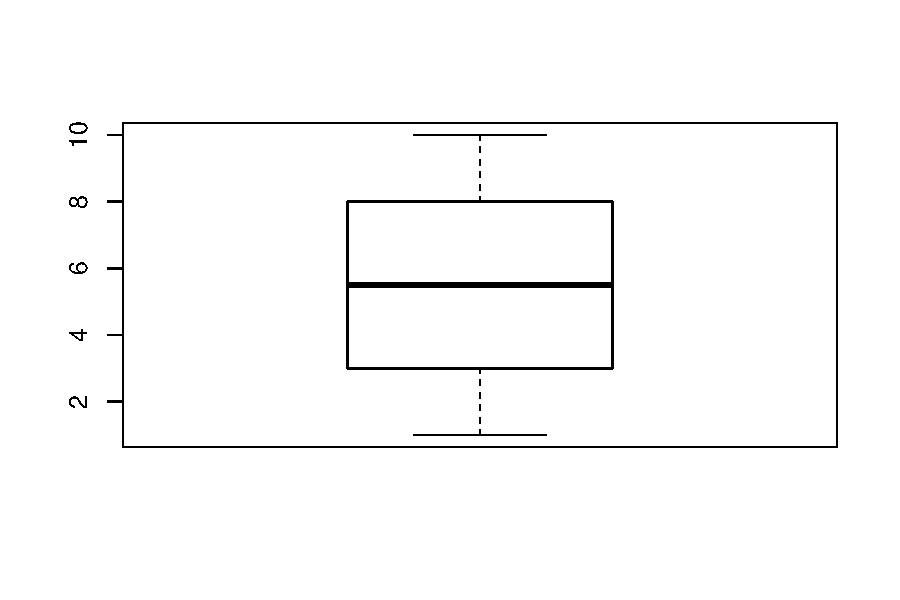
\includegraphics[width=0.5\linewidth]{/Users/serdarbalciold/histopathRprojects/histopathology-template/figs/unnamed-chunk-61-1}
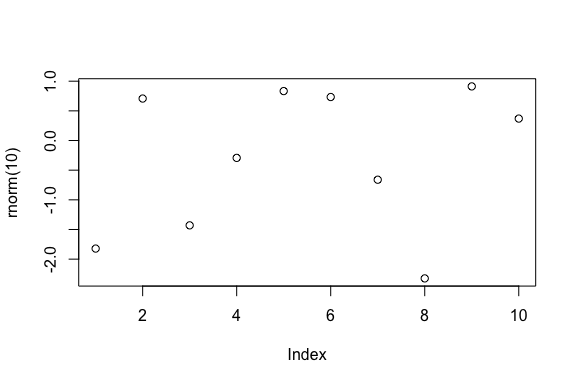
\includegraphics[width=0.5\linewidth]{/Users/serdarbalciold/histopathRprojects/histopathology-template/figs/unnamed-chunk-61-2}

\begin{center}\rule{0.5\linewidth}{0.5pt}\end{center}

Since R Markdown use the
\href{https://getbootstrap.com/docs/4.0/layout/grid/}{bootstrap
framework} under the hood. It is possible to benefit its powerful grid
system. Basically, you can consider that your row is divided in 12
subunits of same width. You can then choose to use only a few of this
subunits.

Here, I use 3 subunits of size 4 (4x3=12). The last column is used for a
plot. You can read more about the grid system
\href{bootstrap\%20grid\%20system}{here}. I got this result showing the
following code in my R Markdown document.

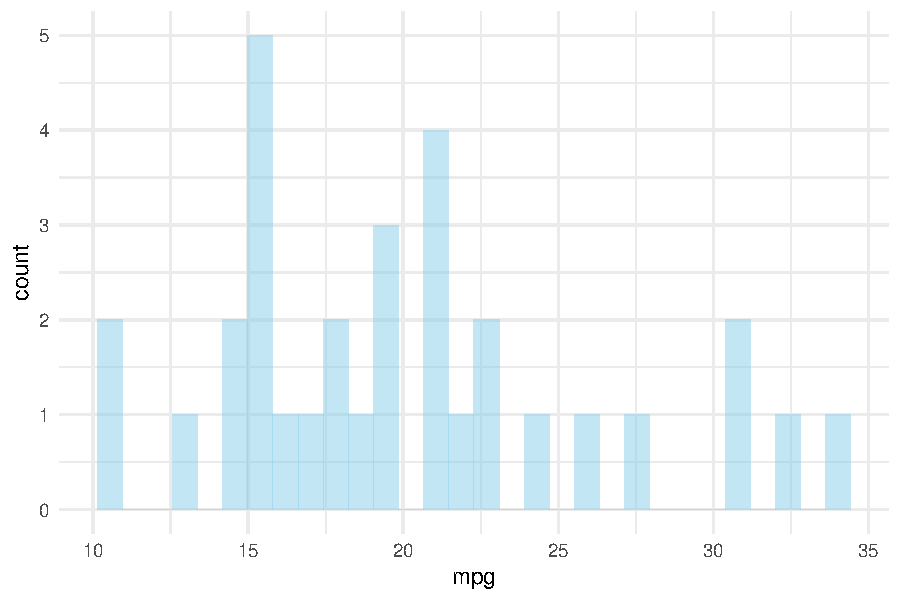
\includegraphics{/Users/serdarbalciold/histopathRprojects/histopathology-template/figs/unnamed-chunk-62-1.pdf}

\begin{center}\rule{0.5\linewidth}{0.5pt}\end{center}

\hypertarget{buttons}{%
\section{Tabs for sub-chapters}\label{buttons}}

\hypertarget{first}{%
\subsection{First}\label{first}}

content of sub-chapter \#1

\hypertarget{second}{%
\subsection{Second}\label{second}}

content of sub-chapter \#2

\hypertarget{third}{%
\subsection{Third}\label{third}}

content of sub-chapter \#3

\begin{center}\rule{0.5\linewidth}{0.5pt}\end{center}

\pagebreak

\hypertarget{discussion}{%
\section{Discussion}\label{discussion}}

\begin{itemize}
\item
  Interpret the results in context of the working hypothesis elaborated
  in the introduction and other relevant studies; include a discussion
  of limitations of the study.
\item
  Discuss potential clinical applications and implications for future
  research
\end{itemize}

\pagebreak

\hypertarget{footer}{%
\section{Footer}\label{footer}}

\textbf{Codes for explaining the software and the packages that are used
in the analysis}\footnote{See
  \href{https://github.com/sbalci/histopathology-template/blob/master/childRmd/_23footer.Rmd}{\texttt{childRmd/\_23footer.Rmd}}
  file for other codes}

\hypertarget{save-final-data}{%
\subsubsection{Save Final Data}\label{save-final-data}}

\begin{Shaded}
\begin{Highlighting}[]
\NormalTok{projectName <-}\StringTok{ }\KeywordTok{list.files}\NormalTok{(}\DataTypeTok{path =}\NormalTok{ here}\OperatorTok{::}\KeywordTok{here}\NormalTok{(), }\DataTypeTok{pattern =} \StringTok{"Rproj"}\NormalTok{)}
\NormalTok{projectName <-}\StringTok{ }\KeywordTok{gsub}\NormalTok{(}\DataTypeTok{pattern =} \StringTok{".Rproj"}\NormalTok{, }\DataTypeTok{replacement =} \StringTok{""}\NormalTok{, }\DataTypeTok{x =}\NormalTok{ projectName)}

\NormalTok{analysisDate <-}\StringTok{ }\KeywordTok{as.character}\NormalTok{(}\KeywordTok{Sys.Date}\NormalTok{())}

\NormalTok{imageName <-}\StringTok{ }\KeywordTok{paste0}\NormalTok{(projectName, analysisDate, }\StringTok{".RData"}\NormalTok{)}

\KeywordTok{save.image}\NormalTok{(}\DataTypeTok{file =}\NormalTok{ here}\OperatorTok{::}\KeywordTok{here}\NormalTok{(}\StringTok{"data"}\NormalTok{, imageName))}

\NormalTok{rdsName <-}\StringTok{ }\KeywordTok{paste0}\NormalTok{(projectName, analysisDate, }\StringTok{".rds"}\NormalTok{)}

\NormalTok{readr}\OperatorTok{::}\KeywordTok{write_rds}\NormalTok{(}\DataTypeTok{x =}\NormalTok{ mydata, }\DataTypeTok{path =}\NormalTok{ here}\OperatorTok{::}\KeywordTok{here}\NormalTok{(}\StringTok{"data"}\NormalTok{, rdsName))}

\KeywordTok{saveRDS}\NormalTok{(}\DataTypeTok{object =}\NormalTok{ mydata, }\DataTypeTok{file =}\NormalTok{ here}\OperatorTok{::}\KeywordTok{here}\NormalTok{(}\StringTok{"data"}\NormalTok{, rdsName))}

\NormalTok{excelName <-}\StringTok{ }\KeywordTok{paste0}\NormalTok{(projectName, analysisDate, }\StringTok{".xlsx"}\NormalTok{)}

\NormalTok{rio}\OperatorTok{::}\KeywordTok{export}\NormalTok{(}\DataTypeTok{x =}\NormalTok{ mydata, }\DataTypeTok{file =}\NormalTok{ here}\OperatorTok{::}\KeywordTok{here}\NormalTok{(}\StringTok{"data"}\NormalTok{, excelName), }\DataTypeTok{format =} \StringTok{"xlsx"}\NormalTok{)}

\CommentTok{# writexl::write_xlsx(mydata, here::here('data', excelName))}

\KeywordTok{print}\NormalTok{(glue}\OperatorTok{::}\KeywordTok{glue}\NormalTok{(}\StringTok{"saved data after analysis to "}\NormalTok{, }\KeywordTok{rownames}\NormalTok{(}\KeywordTok{file.info}\NormalTok{(here}\OperatorTok{::}\KeywordTok{here}\NormalTok{(}\StringTok{"data"}\NormalTok{, }
\NormalTok{    excelName))), }\StringTok{" : "}\NormalTok{, }\KeywordTok{as.character}\NormalTok{(}\KeywordTok{file.info}\NormalTok{(here}\OperatorTok{::}\KeywordTok{here}\NormalTok{(}\StringTok{"data"}\NormalTok{, excelName))}\OperatorTok{$}\NormalTok{ctime)))}
\end{Highlighting}
\end{Shaded}

\begin{verbatim}
saved data after analysis to /Users/serdarbalciold/histopathRprojects/histopathology-template/data/histopathology-template2020-02-26.xlsx : 2020-02-26 14:40:45
\end{verbatim}

\begin{Shaded}
\begin{Highlighting}[]
\NormalTok{mydata }\OperatorTok\StringTok{ }\NormalTok{downloadthis}\OperatorTok{::}\KeywordTok{download_this}\NormalTok{(}\DataTypeTok{output_name =}\NormalTok{ excelName, }\DataTypeTok{output_extension =} \StringTok{".csv"}\NormalTok{, }
    \DataTypeTok{button_label =} \StringTok{"Download data as csv"}\NormalTok{, }\DataTypeTok{button_type =} \StringTok{"default"}\NormalTok{)}
\end{Highlighting}
\end{Shaded}

Download data as csv

\begin{Shaded}
\begin{Highlighting}[]
\NormalTok{mydata }\OperatorTok\StringTok{ }\NormalTok{downloadthis}\OperatorTok{::}\KeywordTok{download_this}\NormalTok{(}\DataTypeTok{output_name =}\NormalTok{ excelName, }\DataTypeTok{output_extension =} \StringTok{".xlsx"}\NormalTok{, }
    \DataTypeTok{button_label =} \StringTok{"Download data as xlsx"}\NormalTok{, }\DataTypeTok{button_type =} \StringTok{"primary"}\NormalTok{)}
\end{Highlighting}
\end{Shaded}

Download data as xlsx

\begin{center}\rule{0.5\linewidth}{0.5pt}\end{center}

\pagebreak

\hypertarget{final-data-summary}{%
\subsubsection{Final Data Summary}\label{final-data-summary}}

\begin{Shaded}
\begin{Highlighting}[]
\CommentTok{# use summarytools to generate final data summary}
\CommentTok{# summarytools::view(summarytools::dfSummary(x = mydata}
\CommentTok{#                                            , style = "markdown"))}
\end{Highlighting}
\end{Shaded}

\begin{center}\rule{0.5\linewidth}{0.5pt}\end{center}

\pagebreak

\hypertarget{software-and-libraries-used}{%
\subsubsection{Software and Libraries
Used}\label{software-and-libraries-used}}

Why and how to cite software and packages?\footnote{Smith AM, Katz DS,
  Niemeyer KE, FORCE11 Software Citation Working Group. (2016) Software
  Citation Principles. PeerJ Computer Science 2:e86. DOI:
  10.7717/peerj-cs.86
  \url{https://www.force11.org/software-citation-principles}}

\begin{Shaded}
\begin{Highlighting}[]
\KeywordTok{citation}\NormalTok{()}
\end{Highlighting}
\end{Shaded}

\begin{verbatim}

To cite R in publications use:

  R Core Team (2019). R: A language and environment for statistical
  computing. R Foundation for Statistical Computing, Vienna, Austria.
  URL https://www.R-project.org/.

A BibTeX entry for LaTeX users is

  @Manual{,
    title = {R: A Language and Environment for Statistical Computing},
    author = {{R Core Team}},
    organization = {R Foundation for Statistical Computing},
    address = {Vienna, Austria},
    year = {2019},
    url = {https://www.R-project.org/},
  }

We have invested a lot of time and effort in creating R, please cite it
when using it for data analysis. See also 'citation("pkgname")' for
citing R packages.
\end{verbatim}

The jamovi project (2019). jamovi. (Version 0.9) {[}Computer
Software{]}. Retrieved from \url{https://www.jamovi.org}.\\
R Core Team (2018). R: A Language and envionment for statistical
computing. {[}Computer software{]}. Retrieved from
\url{https://cran.r-project.org/}.\\
Fox, J., \& Weisberg, S. (2018). car: Companion to Applied Regression.
{[}R package{]}. Retrieved from
\url{https://cran.r-project.org/package=car}. Wickham et al., (2019).
Welcome to the tidyverse. Journal of Open Source Software, 4(43), 1686,
\url{https://doi.org/10.21105/joss.01686} Data processing was carried
out with R (R Core Team, 2019) and the easystats ecosystem (Lüdecke,
Waggoner, \& Makowski, 2019; Makowski, Ben-Shachar, \& Lüdecke, 2019)

\begin{Shaded}
\begin{Highlighting}[]
\NormalTok{report}\OperatorTok{::}\KeywordTok{cite_packages}\NormalTok{(}\DataTypeTok{session =} \KeywordTok{sessionInfo}\NormalTok{())}
\end{Highlighting}
\end{Shaded}

\hypertarget{references}{%
\subsection{References}\label{references}}

Alastair Rushworth (2019). inspectdf: Inspection, Comparison and
Visualisation of Data Frames. R package version 0.0.7.
\url{https://CRAN.R-project.org/package=inspectdf}\\
Alboukadel Kassambara (2020). ggpubr: `ggplot2' Based Publication Ready
Plots. R package version 0.2.5.
\url{https://CRAN.R-project.org/package=ggpubr}\\
Alboukadel Kassambara, Marcin Kosinski and Przemyslaw Biecek (2019).
survminer: Drawing Survival Curves using `ggplot2'. R package version
0.4.6. \url{https://CRAN.R-project.org/package=survminer}\\
Benjamin Elbers (2020). tidylog: Logging for `dplyr' and `tidyr'
Functions. R package version 1.0.0.
\url{https://CRAN.R-project.org/package=tidylog}\\
Boxuan Cui (2020). DataExplorer: Automate Data Exploration and
Treatment. R package version 0.8.1.
\url{https://CRAN.R-project.org/package=DataExplorer}\\
Chung-hong Chan, Geoffrey CH Chan, Thomas J. Leeper, and Jason Becker
(2018). rio: A Swiss-army knife for data file I/O. R package version
0.5.16.\\
David Robinson and Alex Hayes (2020). broom: Convert Statistical
Analysis Objects into Tidy Tibbles. R package version 0.5.4.
\url{https://CRAN.R-project.org/package=broom}\\
Dayanand Ubrangala, Kiran R, Ravi Prasad Kondapalli and Sayan Putatunda
(2020). SmartEDA: Summarize and Explore the Data. R package version
0.3.3. \url{https://CRAN.R-project.org/package=SmartEDA}\\
Dirk Eddelbuettel and Romain Francois (2011). Rcpp: Seamless R and C++
Integration. Journal of Statistical Software, 40(8), 1-18. URL
\url{http://www.jstatsoft.org/v40/i08/}.\\
Dirk Eddelbuettel with contributions by Antoine Lucas, Jarek Tuszynski,
Henrik Bengtsson, Simon Urbanek, Mario Frasca, Bryan Lewis, Murray
Stokely, Hannes Muehleisen, Duncan Murdoch, Jim Hester, Wush Wu, Qiang
Kou, Thierry Onkelinx, Michel Lang, Viliam Simko, Kurt Hornik, Radford
Neal, Kendon Bell, Matthew de Queljoe, Ion Suruceanu and Bill Denney.
(2020). digest: Create Compact Hash Digests of R Objects. R package
version 0.6.24. \url{https://CRAN.R-project.org/package=digest} Ethan
Heinzen, Jason Sinnwell, Elizabeth Atkinson, Tina Gunderson and Gregory
Dougherty (2020). arsenal: An Arsenal of `R' Functions for Large-Scale
Statistical Summaries. R package version 3.4.0.
\url{https://CRAN.R-project.org/package=arsenal}\\
Ewen Harrison, Tom Drake and Riinu Ots (2019). finalfit: Quickly Create
Elegant Regression Results Tables and Plots when Modelling. R package
version 0.9.7. \url{https://CRAN.R-project.org/package=finalfit}\\
Garrett Grolemund, Hadley Wickham (2011). Dates and Times Made Easy with
lubridate. Journal of Statistical Software, 40(3), 1-25. URL
\url{http://www.jstatsoft.org/v40/i03/}.\\
H. Wickham. ggplot2: Elegant Graphics for Data Analysis. Springer-Verlag
New York, 2016.\\
Hadley Wickham (2019). feather: R Bindings to the Feather `API'. R
package version 0.3.5.
\url{https://CRAN.R-project.org/package=feather}\\
Hadley Wickham (2019). forcats: Tools for Working with Categorical
Variables (Factors). R package version 0.4.0.
\url{https://CRAN.R-project.org/package=forcats}\\
Hadley Wickham (2019). httr: Tools for Working with URLs and HTTP. R
package version 1.4.1. \url{https://CRAN.R-project.org/package=httr}\\
Hadley Wickham (2019). modelr: Modelling Functions that Work with the
Pipe. R package version 0.1.5.
\url{https://CRAN.R-project.org/package=modelr}\\
Hadley Wickham (2019). rvest: Easily Harvest (Scrape) Web Pages. R
package version 0.3.5. \url{https://CRAN.R-project.org/package=rvest}\\
Hadley Wickham (2019). stringr: Simple, Consistent Wrappers for Common
String Operations. R package version 1.4.0.
\url{https://CRAN.R-project.org/package=stringr}\\
Hadley Wickham and Evan Miller (2019). haven: Import and Export `SPSS',
`Stata' and `SAS' Files. R package version 2.2.0.
\url{https://CRAN.R-project.org/package=haven}\\
Hadley Wickham and Jennifer Bryan (2019). readxl: Read Excel Files. R
package version 1.3.1. \url{https://CRAN.R-project.org/package=readxl}\\
Hadley Wickham and Lionel Henry (2020). tidyr: Tidy Messy Data. R
package version 1.0.2. \url{https://CRAN.R-project.org/package=tidyr}\\
Hadley Wickham and Yihui Xie (2019). evaluate: Parsing and Evaluation
Tools that Provide More Details than the Default. R package version
0.14. \url{https://CRAN.R-project.org/package=evaluate}\\
Hadley Wickham, Jim Hester and Jeroen Ooms (2019). xml2: Parse XML. R
package version 1.2.2. \url{https://CRAN.R-project.org/package=xml2}\\
Hadley Wickham, Jim Hester and Romain Francois (2018). readr: Read
Rectangular Text Data. R package version 1.3.1.
\url{https://CRAN.R-project.org/package=readr}\\
Hadley Wickham, Romain François, Lionel Henry and Kirill Müller (2020).
dplyr: A Grammar of Data Manipulation. R package version 0.8.4.
\url{https://CRAN.R-project.org/package=dplyr}\\
Jeremy Stephens, Kirill Simonov, Yihui Xie, Zhuoer Dong, Hadley Wickham,
Jeffrey Horner, reikoch, Will Beasley, Brendan O'Connor and Gregory R.
Warnes (2020). yaml: Methods to Convert R Data to YAML and Back. R
package version 2.2.1. \url{https://CRAN.R-project.org/package=yaml}\\
Jeroen Ooms (2014). The jsonlite Package: A Practical and Consistent
Mapping Between JSON Data and R Objects. arXiv:1403.2805 {[}stat.CO{]}
URL \url{https://arxiv.org/abs/1403.2805}.\\
Jim Hester (2019). glue: Interpreted String Literals. R package version
1.3.1. \url{https://CRAN.R-project.org/package=glue}\\
Jim Hester and Gábor Csárdi (2019). pak: Another Approach to Package
Installation. R package version 0.1.2.
\url{https://CRAN.R-project.org/package=pak}\\
Jim Hester, Gábor Csárdi, Hadley Wickham, Winston Chang, Martin Morgan
and Dan Tenenbaum (2020). remotes: R Package Installation from Remote
Repositories, Including `GitHub'. R package version 2.1.1.
\url{https://CRAN.R-project.org/package=remotes}\\
JJ Allaire and Yihui Xie and Jonathan McPherson and Javier Luraschi and
Kevin Ushey and Aron Atkins and Hadley Wickham and Joe Cheng and Winston
Chang and Richard Iannone (2020). rmarkdown: Dynamic Documents for R. R
package version 2.1. URL \url{https://rmarkdown.rstudio.com}.\\
JJ Allaire, Jeffrey Horner, Yihui Xie, Vicent Marti and Natacha Porte
(2019). markdown: Render Markdown with the C Library `Sundown'. R
package version 1.1. \url{https://CRAN.R-project.org/package=markdown}\\
Kazuki Yoshida (2019). tableone: Create `Table 1' to Describe Baseline
Characteristics. R package version 0.10.0.
\url{https://CRAN.R-project.org/package=tableone}\\
Kevin Ushey (2020). renv: Project Environments. R package version 0.9.3.
\url{https://CRAN.R-project.org/package=renv}\\
Kirill Müller (2017). here: A Simpler Way to Find Your Files. R package
version 0.1. \url{https://CRAN.R-project.org/package=here}\\
Kirill Müller (2020). hms: Pretty Time of Day. R package version 0.5.3.
\url{https://CRAN.R-project.org/package=hms}\\
Kirill Müller and Hadley Wickham (2019). tibble: Simple Data Frames. R
package version 2.1.3. \url{https://CRAN.R-project.org/package=tibble}\\
Koji Makiyama (2016). magicfor: Magic Functions to Obtain Results from
for Loops. R package version 0.1.0.
\url{https://CRAN.R-project.org/package=magicfor}\\
Lionel Henry and Hadley Wickham (2019). purrr: Functional Programming
Tools. R package version 0.3.3.
\url{https://CRAN.R-project.org/package=purrr}\\
Lionel Henry and Hadley Wickham (2020). rlang: Functions for Base Types
and Core R and `Tidyverse' Features. R package version 0.4.4.
\url{https://CRAN.R-project.org/package=rlang}\\
Makowski, D. \& Lüdecke, D. (2019). The report package for R: Ensuring
the use of best practices for results reporting. CRAN. Available from
\url{https://github.com/easystats/report}. doi: .\\
Pablo Seibelt (2017). xray: X Ray Vision on your Datasets. R package
version 0.2. \url{https://CRAN.R-project.org/package=xray}\\
Paul Hendricks (2015). describer: Describe Data in R Using Common
Descriptive Statistics. R package version 0.2.0.
\url{https://CRAN.R-project.org/package=describer}\\
Petersen AH, Ekstrøm CT (2019). ``dataMaid: Your Assistant
forDocumenting Supervised Data Quality Screening in R.'' \emph{Journal
ofStatistical Software}, \emph{90}(6), 1-38. doi: 10.18637/jss.v090.i06
(URL:\url{https://doi.org/10.18637/jss.v090.i06}).\\
Rinker, T. W. (2018). wakefield: Generate Random Data. version 0.3.3.
Buffalo, New York. \url{https://github.com/trinker/wakefield}\\
Rinker, T. W. \& Kurkiewicz, D. (2017). pacman: Package Management for
R. version 0.5.0. Buffalo, New York.
\url{http://github.com/trinker/pacman}\\
Roland Krasser (2020). explore: Simplifies Exploratory Data Analysis. R
package version 0.5.4.
\url{https://CRAN.R-project.org/package=explore}\\
RStudio and Inc.~(2019). htmltools: Tools for HTML. R package version
0.4.0. \url{https://CRAN.R-project.org/package=htmltools}\\
Sam Firke (2020). janitor: Simple Tools for Examining and Cleaning Dirty
Data. R package version 1.2.1.
\url{https://CRAN.R-project.org/package=janitor}\\
Simon Urbanek (2015). base64enc: Tools for base64 encoding. R package
version 0.1-3. \url{https://CRAN.R-project.org/package=base64enc}\\
Stefan Milton Bache and Hadley Wickham (2014). magrittr: A Forward-Pipe
Operator for R. R package version 1.5.
\url{https://CRAN.R-project.org/package=magrittr}\\
Therneau T (2015). \emph{A Package for Survival Analysis in S}.
version2.38, \textless URL:
\url{https://CRAN.R-project.org/package=survival}\textgreater.\\
Tierney N (2017). ``visdat: Visualising Whole Data Frames.''
\emph{JOSS},\emph{2}(16), 355. doi: 10.21105/joss.00355
(URL:\url{https://doi.org/10.21105/joss.00355}),
\textless URL:\url{http://dx.doi.org/10.21105/joss.00355}\textgreater.\\
Yihui Xie (2019). formatR: Format R Code Automatically. R package
version 1.7. \url{https://CRAN.R-project.org/package=formatR}\\
Yihui Xie (2020). knitr: A General-Purpose Package for Dynamic Report
Generation in R. R package version 1.28.\\
Yihui Xie (2020). mime: Map Filenames to MIME Types. R package version
0.9. \url{https://CRAN.R-project.org/package=mime}\\
Yixuan Qiu and Yihui Xie (2019). highr: Syntax Highlighting for R Source
Code. R package version 0.8.
\url{https://CRAN.R-project.org/package=highr}

\begin{Shaded}
\begin{Highlighting}[]
\NormalTok{report}\OperatorTok{::}\KeywordTok{show_packages}\NormalTok{(}\DataTypeTok{session =} \KeywordTok{sessionInfo}\NormalTok{()) }\OperatorTok\StringTok{ }\NormalTok{kableExtra}\OperatorTok{::}\KeywordTok{kable}\NormalTok{()}
\end{Highlighting}
\end{Shaded}

\begin{Shaded}
\begin{Highlighting}[]
\CommentTok{# citation('tidyverse')}
\KeywordTok{citation}\NormalTok{(}\StringTok{"readxl"}\NormalTok{)}
\end{Highlighting}
\end{Shaded}

\begin{verbatim}

To cite package 'readxl' in publications use:

  Hadley Wickham and Jennifer Bryan (2019). readxl: Read Excel Files. R
  package version 1.3.1. https://CRAN.R-project.org/package=readxl

A BibTeX entry for LaTeX users is

  @Manual{,
    title = {readxl: Read Excel Files},
    author = {Hadley Wickham and Jennifer Bryan},
    year = {2019},
    note = {R package version 1.3.1},
    url = {https://CRAN.R-project.org/package=readxl},
  }
\end{verbatim}

\begin{Shaded}
\begin{Highlighting}[]
\KeywordTok{citation}\NormalTok{(}\StringTok{"janitor"}\NormalTok{)}
\end{Highlighting}
\end{Shaded}

\begin{verbatim}

To cite package 'janitor' in publications use:

  Sam Firke (2020). janitor: Simple Tools for Examining and Cleaning
  Dirty Data. R package version 1.2.1.
  https://CRAN.R-project.org/package=janitor

A BibTeX entry for LaTeX users is

  @Manual{,
    title = {janitor: Simple Tools for Examining and Cleaning Dirty Data},
    author = {Sam Firke},
    year = {2020},
    note = {R package version 1.2.1},
    url = {https://CRAN.R-project.org/package=janitor},
  }
\end{verbatim}

\begin{Shaded}
\begin{Highlighting}[]
\CommentTok{# citation('report')}
\KeywordTok{citation}\NormalTok{(}\StringTok{"finalfit"}\NormalTok{)}
\end{Highlighting}
\end{Shaded}

\begin{verbatim}

To cite package 'finalfit' in publications use:

  Ewen Harrison, Tom Drake and Riinu Ots (2019). finalfit: Quickly
  Create Elegant Regression Results Tables and Plots when Modelling. R
  package version 0.9.7. https://CRAN.R-project.org/package=finalfit

A BibTeX entry for LaTeX users is

  @Manual{,
    title = {finalfit: Quickly Create Elegant Regression Results Tables and Plots when
Modelling},
    author = {Ewen Harrison and Tom Drake and Riinu Ots},
    year = {2019},
    note = {R package version 0.9.7},
    url = {https://CRAN.R-project.org/package=finalfit},
  }
\end{verbatim}

\begin{Shaded}
\begin{Highlighting}[]
\CommentTok{# citation('ggstatsplot')}
\end{Highlighting}
\end{Shaded}

\begin{Shaded}
\begin{Highlighting}[]
\ControlFlowTok{if}\NormalTok{ (}\OperatorTok{!}\KeywordTok{dir.exists}\NormalTok{(here}\OperatorTok{::}\KeywordTok{here}\NormalTok{(}\StringTok{"bib"}\NormalTok{))) \{}
    \KeywordTok{dir.create}\NormalTok{(here}\OperatorTok{::}\KeywordTok{here}\NormalTok{(}\StringTok{"bib"}\NormalTok{))}
\NormalTok{\}}

\NormalTok{knitr}\OperatorTok{::}\KeywordTok{write_bib}\NormalTok{(}\DataTypeTok{x =} \KeywordTok{c}\NormalTok{(}\KeywordTok{.packages}\NormalTok{(), }\StringTok{"knitr"}\NormalTok{, }\StringTok{"shiny"}\NormalTok{), }\DataTypeTok{file =}\NormalTok{ here}\OperatorTok{::}\KeywordTok{here}\NormalTok{(}\StringTok{"bib"}\NormalTok{, }\StringTok{"packages.bib"}\NormalTok{))}
\end{Highlighting}
\end{Shaded}

\begin{center}\rule{0.5\linewidth}{0.5pt}\end{center}

\pagebreak

\hypertarget{session-info}{%
\subsubsection{Session Info}\label{session-info}}

\begin{Shaded}
\begin{Highlighting}[]
\KeywordTok{sessionInfo}\NormalTok{()}
\end{Highlighting}
\end{Shaded}

\begin{verbatim}
R version 3.6.0 (2019-04-26)
Platform: x86_64-apple-darwin15.6.0 (64-bit)
Running under: macOS  10.15.3

Matrix products: default
BLAS:   /Library/Frameworks/R.framework/Versions/3.6/Resources/lib/libRblas.0.dylib
LAPACK: /Library/Frameworks/R.framework/Versions/3.6/Resources/lib/libRlapack.dylib

locale:
[1] en_US.UTF-8/en_US.UTF-8/en_US.UTF-8/C/en_US.UTF-8/en_US.UTF-8

attached base packages:
[1] stats     graphics  grDevices datasets  utils     methods   base     

other attached packages:
 [1] survminer_0.4.6    ggpubr_0.2.5       survival_3.1-8     magrittr_1.5      
 [5] report_0.1.0       wakefield_0.3.3    SmartEDA_0.3.3     magicfor_0.1.0    
 [9] tableone_0.10.0    arsenal_3.4.0      DataExplorer_0.8.1 xray_0.2          
[13] visdat_0.5.3       inspectdf_0.0.7    describer_0.2.0    dataMaid_1.4.0    
[17] finalfit_0.9.7     explore_0.5.4      rio_0.5.16         janitor_1.2.1     
[21] formatR_1.7        renv_0.9.3         rlang_0.4.4        glue_1.3.1        
[25] tidylog_1.0.0      broom_0.5.4        modelr_0.1.5       rvest_0.3.5       
[29] xml2_1.2.2         readxl_1.3.1       httr_1.4.1         haven_2.2.0       
[33] feather_0.3.5      lubridate_1.7.4    hms_0.5.3          forcats_0.4.0     
[37] stringr_1.4.0      tibble_2.1.3       purrr_0.3.3        readr_1.3.1       
[41] tidyr_1.0.2        dplyr_0.8.4        ggplot2_3.2.1      rmarkdown_2.1     
[45] mime_0.9           base64enc_0.1-3    jsonlite_1.6.1     htmltools_0.4.0   
[49] Rcpp_1.0.3         yaml_2.2.1         markdown_1.1       highr_0.8         
[53] digest_0.6.24      evaluate_0.14      knitr_1.28         here_0.1          
[57] pak_0.1.2          pacman_0.5.1       remotes_2.1.1     

loaded via a namespace (and not attached):
  [1] utf8_1.1.4          tidyselect_1.0.0    lme4_1.1-21        
  [4] htmlwidgets_1.5.1   grid_3.6.0          lpSolve_5.6.15     
  [7] munsell_0.5.0       effectsize_0.1.2    codetools_0.2-16   
 [10] DT_0.12.1           withr_2.1.2         ISLR_1.2           
 [13] colorspace_1.4-1    rstudioapi_0.11     robustbase_0.93-5  
 [16] ggsignif_0.6.0      labeling_0.3        KMsurv_0.1-5       
 [19] farver_2.0.3        rprojroot_1.3-2     vctrs_0.2.3        
 [22] generics_0.0.2      xfun_0.12           downloadthis_0.1.0 
 [25] R6_2.4.1            reshape_0.8.8       assertthat_0.2.1   
 [28] promises_1.1.0      networkD3_0.4       scales_1.1.0       
 [31] nnet_7.3-12         gtable_0.3.0        processx_3.4.2     
 [34] clisymbols_1.2.0    whoami_1.3.0        splines_3.6.0      
 [37] lazyeval_0.2.2      acepack_1.4.1       bsplus_0.1.1       
 [40] checkmate_2.0.0     backports_1.1.5     httpuv_1.5.2       
 [43] Hmisc_4.3-1         tools_3.6.0         ellipsis_0.3.0     
 [46] RColorBrewer_1.1-2  plyr_1.8.5          jmvcore_1.2.5      
 [49] progress_1.2.2      ps_1.3.2            prettyunits_1.1.1  
 [52] rpart_4.1-15        sampling_2.8        zoo_1.8-7          
 [55] reactR_0.4.2        cluster_2.1.0       fs_1.3.1           
 [58] survey_3.37         data.table_1.12.8   openxlsx_4.1.4     
 [61] mitml_0.3-7         reactable_0.1.0     xtable_1.8-4       
 [64] jpeg_0.1-8.1        gridExtra_2.3       compiler_3.6.0     
 [67] mice_3.7.0          writexl_1.2         crayon_1.3.4       
 [70] minqa_1.2.4         later_1.0.0         Formula_1.2-3      
 [73] DBI_1.1.0           jmv_1.2.5           MASS_7.3-51.5      
 [76] boot_1.3-24         Matrix_1.2-18       cli_2.0.1          
 [79] mitools_2.4         parallel_3.6.0      insight_0.8.1      
 [82] pan_1.6             igraph_1.2.4.2      pkgconfig_2.0.3    
 [85] km.ci_0.5-2         foreign_0.8-75      foreach_1.4.8      
 [88] webshot_0.5.2       snakecase_0.11.0    callr_3.4.2        
 [91] parameters_0.5.0.1  cellranger_1.1.0    survMisc_0.5.5     
 [94] htmlTable_1.13.3    curl_4.3            shiny_1.4.0        
 [97] jomo_2.6-10         rjson_0.2.20        nloptr_1.2.1       
[100] lifecycle_0.1.0     nlme_3.1-144        fansi_0.4.1        
[103] labelled_2.2.2      pillar_1.4.3        ggsci_2.9          
[106] lattice_0.20-38     GGally_1.4.0        fastmap_1.0.1      
[109] DEoptimR_1.0-8      bayestestR_0.5.2    zip_2.0.4          
[112] png_0.1-7           iterators_1.0.12    pander_0.6.3       
[115] performance_0.4.4   class_7.3-15        stringi_1.4.6      
[118] ggfittext_0.8.1     latticeExtra_0.6-29 e1071_1.7-3        
\end{verbatim}

\pagebreak

\begin{center}\rule{0.5\linewidth}{0.5pt}\end{center}

\hypertarget{loaded-packages}{%
\subsubsection{Loaded packages}\label{loaded-packages}}

\begin{Shaded}
\begin{Highlighting}[]
\NormalTok{pacman}\OperatorTok{::}\KeywordTok{p_loaded}\NormalTok{(}\DataTypeTok{all =} \OtherTok{TRUE}\NormalTok{)}
\end{Highlighting}
\end{Shaded}

\begin{center}\rule{0.5\linewidth}{0.5pt}\end{center}

\pagebreak

\hypertarget{notes}{%
\subsubsection{Notes}\label{notes}}

Last update on \$ 2020-02-26 21:18:37 \$

Serdar Balci, MD, Pathologist\\
\href{mailto:drserdarbalci@gmail.com}{\nolinkurl{drserdarbalci@gmail.com}}\\
\url{https://rpubs.com/sbalci/CV}

\begin{center}\rule{0.5\linewidth}{0.5pt}\end{center}

\pagebreak

\hypertarget{code-appendix}{%
\subsection{Code Appendix}\label{code-appendix}}

\textbf{Use following chunk options to include all codes below the
report.}

\begin{Shaded}
\begin{Highlighting}[]
\NormalTok{\{r, echo=}\OtherTok{TRUE}\NormalTok{, eval=}\OtherTok{FALSE}\NormalTok{, ref.label=knitr}\OperatorTok{::}\KeywordTok{all_labels}\NormalTok{()\}}
\end{Highlighting}
\end{Shaded}

\begin{Shaded}
\begin{Highlighting}[]
\CommentTok{# installing necessary packages}
\ControlFlowTok{if}\NormalTok{ (}\KeywordTok{requireNamespace}\NormalTok{(}\StringTok{"magrittr"}\NormalTok{, }\DataTypeTok{quietly =} \OtherTok{TRUE}\NormalTok{)) \{}
  \StringTok{`}\DataTypeTok\StringTok{`}\NormalTok{ <-}\StringTok{ }\NormalTok{magrittr}\OperatorTok{::}\StringTok{`}\DataTypeTok\StringTok{`}
\NormalTok{\}}
\ControlFlowTok{if}\NormalTok{ (}\OperatorTok{!}\KeywordTok{require}\NormalTok{(}\StringTok{"remotes"}\NormalTok{)) }\KeywordTok{install.packages}\NormalTok{(}\StringTok{"remotes"}\NormalTok{)}
\ControlFlowTok{if}\NormalTok{ (}\OperatorTok{!}\KeywordTok{require}\NormalTok{(}\StringTok{"pacman"}\NormalTok{)) }\KeywordTok{install.packages}\NormalTok{(}\StringTok{"pacman"}\NormalTok{)}
\ControlFlowTok{if}\NormalTok{ (}\OperatorTok{!}\KeywordTok{require}\NormalTok{(}\StringTok{"pak"}\NormalTok{)) }\KeywordTok{install.packages}\NormalTok{(}\StringTok{"pak"}\NormalTok{)}
\ControlFlowTok{if}\NormalTok{ (}\OperatorTok{!}\KeywordTok{require}\NormalTok{(}\StringTok{"here"}\NormalTok{)) }\KeywordTok{install.packages}\NormalTok{(}\StringTok{"here"}\NormalTok{)}
\NormalTok{source_rmd <-}\StringTok{ }\ControlFlowTok{function}\NormalTok{(rmd_file)\{}
\NormalTok{  knitr}\OperatorTok{::}\KeywordTok{knit}\NormalTok{(rmd_file, }\DataTypeTok{output =} \KeywordTok{tempfile}\NormalTok{(), }\DataTypeTok{envir =} \KeywordTok{globalenv}\NormalTok{())}
\NormalTok{\}}

\NormalTok{list_of_Rmd <-}\StringTok{ }\KeywordTok{list.files}\NormalTok{(}\DataTypeTok{path =}\NormalTok{ here}\OperatorTok{::}\KeywordTok{here}\NormalTok{(}\StringTok{"childRmd"}\NormalTok{), }\DataTypeTok{pattern =} \StringTok{"Rmd"}\NormalTok{)}

\NormalTok{list_of_Rmd <-}\StringTok{ }\NormalTok{list_of_Rmd[}\OperatorTok{!}\NormalTok{list_of_Rmd }\OperatorTok\StringTok{ }\KeywordTok{c}\NormalTok{(}\StringTok{"_19shinySurvival.Rmd"}\NormalTok{)]}

\NormalTok{purrr}\OperatorTok{::}\KeywordTok{map}\NormalTok{(}\DataTypeTok{.x =}\NormalTok{ here}\OperatorTok{::}\KeywordTok{here}\NormalTok{(}\StringTok{"childRmd"}\NormalTok{, list_of_Rmd), }\DataTypeTok{.f =}\NormalTok{ source_rmd)}

\KeywordTok{source}\NormalTok{(}\DataTypeTok{file =}\NormalTok{ here}\OperatorTok{::}\KeywordTok{here}\NormalTok{(}\StringTok{"R"}\NormalTok{, }\StringTok{"force_git.R"}\NormalTok{))}
\NormalTok{knitr}\OperatorTok{::}\NormalTok{opts_chunk}\OperatorTok{$}\KeywordTok{set}\NormalTok{(}
    \DataTypeTok{eval =} \OtherTok{TRUE}\NormalTok{,}
    \DataTypeTok{echo =} \OtherTok{TRUE}\NormalTok{,}
    \DataTypeTok{fig.path =}\NormalTok{ here}\OperatorTok{::}\KeywordTok{here}\NormalTok{(}\StringTok{"figs/"}\NormalTok{),}
    \DataTypeTok{message =} \OtherTok{FALSE}\NormalTok{,}
    \DataTypeTok{warning =} \OtherTok{FALSE}\NormalTok{,}
    \DataTypeTok{error =} \OtherTok{TRUE}\NormalTok{,}
    \DataTypeTok{cache =} \OtherTok{TRUE}\NormalTok{,}
    \DataTypeTok{comment =} \OtherTok{NA}\NormalTok{,}
    \DataTypeTok{tidy =} \OtherTok{TRUE}\NormalTok{,}
    \DataTypeTok{fig.width =} \DecValTok{6}\NormalTok{,}
    \DataTypeTok{fig.height =} \DecValTok{4}
\NormalTok{)}
\KeywordTok{library}\NormalTok{(knitr)}
\NormalTok{hook_output =}\StringTok{ }\NormalTok{knit_hooks}\OperatorTok{$}\KeywordTok{get}\NormalTok{(}\StringTok{'output'}\NormalTok{)}
\NormalTok{knit_hooks}\OperatorTok{$}\KeywordTok{set}\NormalTok{(}\DataTypeTok{output =} \ControlFlowTok{function}\NormalTok{(x, options) \{}
  \CommentTok{# this hook is used only when the linewidth option is not NULL}
  \ControlFlowTok{if}\NormalTok{ (}\OperatorTok{!}\KeywordTok{is.null}\NormalTok{(n <-}\StringTok{ }\NormalTok{options}\OperatorTok{$}\NormalTok{linewidth)) \{}
\NormalTok{    x =}\StringTok{ }\NormalTok{knitr}\OperatorTok{:::}\KeywordTok{split_lines}\NormalTok{(x)}
    \CommentTok{# any lines wider than n should be wrapped}
    \ControlFlowTok{if}\NormalTok{ (}\KeywordTok{any}\NormalTok{(}\KeywordTok{nchar}\NormalTok{(x) }\OperatorTok{>}\StringTok{ }\NormalTok{n)) x =}\StringTok{ }\KeywordTok{strwrap}\NormalTok{(x, }\DataTypeTok{width =}\NormalTok{ n)}
\NormalTok{    x =}\StringTok{ }\KeywordTok{paste}\NormalTok{(x, }\DataTypeTok{collapse =} \StringTok{'}\CharTok{\textbackslash{}n}\StringTok{'}\NormalTok{)}
\NormalTok{  \}}
  \KeywordTok{hook_output}\NormalTok{(x, options)}
\NormalTok{\})}
\CommentTok{# linewidth css}
\NormalTok{  pre}\OperatorTok{:}\KeywordTok{not}\NormalTok{([class]) \{}
\NormalTok{    color}\OperatorTok{:}\StringTok{ }\CommentTok{#333333;}
\StringTok{    }\NormalTok{background}\OperatorTok{-}\NormalTok{color}\OperatorTok{:}\StringTok{ }\CommentTok{#cccccc;}
\StringTok{  }\NormalTok{\}}
\CommentTok{# linewidth css}
\CommentTok{# https://cran.r-project.org/web/packages/exploreR/vignettes/exploreR.html}
\CommentTok{# exploreR::reset()}
\KeywordTok{source}\NormalTok{(}\DataTypeTok{file =}\NormalTok{ here}\OperatorTok{::}\KeywordTok{here}\NormalTok{(}\StringTok{"R"}\NormalTok{, }\StringTok{"loadLibrary.R"}\NormalTok{))}
\KeywordTok{source}\NormalTok{(}\DataTypeTok{file =}\NormalTok{ here}\OperatorTok{::}\KeywordTok{here}\NormalTok{(}\StringTok{"R"}\NormalTok{, }\StringTok{"gc_fake_data.R"}\NormalTok{))}
\NormalTok{wakefield}\OperatorTok{::}\KeywordTok{table_heat}\NormalTok{(}\DataTypeTok{x =}\NormalTok{ fakedata, }\DataTypeTok{palette =} \StringTok{"Set1"}\NormalTok{, }\DataTypeTok{flip =} \OtherTok{TRUE}\NormalTok{, }\DataTypeTok{print =} \OtherTok{TRUE}\NormalTok{)}
\KeywordTok{library}\NormalTok{(readxl)}
\NormalTok{mydata <-}\StringTok{ }\NormalTok{readxl}\OperatorTok{::}\KeywordTok{read_excel}\NormalTok{(here}\OperatorTok{::}\KeywordTok{here}\NormalTok{(}\StringTok{"data"}\NormalTok{, }\StringTok{"mydata.xlsx"}\NormalTok{))}
\CommentTok{# View(mydata) # Use to view data after importing}
\CommentTok{# https://cran.r-project.org/web/packages/rio/vignettes/rio.html}
\CommentTok{# rio::install_formats()}

\NormalTok{x <-}\StringTok{ }\NormalTok{rio}\OperatorTok{::}\KeywordTok{import}\NormalTok{(}\StringTok{"mtcars.csv"}\NormalTok{)}
\NormalTok{y <-}\StringTok{ }\NormalTok{rio}\OperatorTok{::}\KeywordTok{import}\NormalTok{(}\StringTok{"mtcars.rds"}\NormalTok{)}
\NormalTok{z <-}\StringTok{ }\NormalTok{rio}\OperatorTok{::}\KeywordTok{import}\NormalTok{(}\StringTok{"mtcars.dta"}\NormalTok{)}

\NormalTok{rio}\OperatorTok{::}\KeywordTok{import}\NormalTok{(}\StringTok{"mtcars_noext"}\NormalTok{, }\DataTypeTok{format =} \StringTok{"csv"}\NormalTok{)}

\NormalTok{rio}\OperatorTok{::}\KeywordTok{export}\NormalTok{(mtcars, }\StringTok{"mtcars.csv"}\NormalTok{)}
\NormalTok{rio}\OperatorTok{::}\KeywordTok{export}\NormalTok{(mtcars, }\StringTok{"mtcars.rds"}\NormalTok{)}
\NormalTok{rio}\OperatorTok{::}\KeywordTok{export}\NormalTok{(mtcars, }\StringTok{"mtcars.dta"}\NormalTok{)}

\NormalTok{rio}\OperatorTok{::}\KeywordTok{export}\NormalTok{(}\KeywordTok{list}\NormalTok{(}\DataTypeTok{mtcars =}\NormalTok{ mtcars, }\DataTypeTok{iris =}\NormalTok{ iris), }\StringTok{"multi.xlsx"}\NormalTok{)}

\CommentTok{# Dataframe report}
\NormalTok{mydata }\OperatorTok\StringTok{ }
\StringTok{  }\NormalTok{dplyr}\OperatorTok{::}\KeywordTok{select}\NormalTok{(}\OperatorTok{-}\KeywordTok{contains}\NormalTok{(}\StringTok{"Date"}\NormalTok{)) }\OperatorTok
\StringTok{  }\NormalTok{report}\OperatorTok{::}\KeywordTok{report}\NormalTok{(.)}
\NormalTok{mydata }\OperatorTok\StringTok{ }\NormalTok{explore}\OperatorTok{::}\KeywordTok{describe_tbl}\NormalTok{()}
\KeywordTok{dput}\NormalTok{(}\KeywordTok{names}\NormalTok{(mydata))}
\NormalTok{keycolumns <-}\StringTok{  }
\StringTok{    }\NormalTok{mydata }\OperatorTok\StringTok{  }
\StringTok{    }\KeywordTok{sapply}\NormalTok{(., }\DataTypeTok{FUN =}\NormalTok{ dataMaid}\OperatorTok{::}\NormalTok{isKey) }\OperatorTok\StringTok{  }
\StringTok{    }\NormalTok{tibble}\OperatorTok{::}\KeywordTok{as_tibble}\NormalTok{() }\OperatorTok\StringTok{  }
\StringTok{    }\NormalTok{dplyr}\OperatorTok{::}\KeywordTok{select}\NormalTok{(  }
        \KeywordTok{which}\NormalTok{(.[}\DecValTok{1}\NormalTok{, ] }\OperatorTok{==}\StringTok{ }\OtherTok{TRUE}\NormalTok{)  }
\NormalTok{    ) }\OperatorTok\StringTok{   }
\StringTok{    }\KeywordTok{names}\NormalTok{()  }
\NormalTok{keycolumns  }
\NormalTok{mydata }\OperatorTok\StringTok{ }
\StringTok{  }\NormalTok{dplyr}\OperatorTok{::}\KeywordTok{select}\NormalTok{(}\OperatorTok{-}\NormalTok{keycolumns) }\OperatorTok\StringTok{ }
\NormalTok{inspectdf}\OperatorTok{::}\KeywordTok{inspect_types}\NormalTok{()}
\NormalTok{mydata }\OperatorTok\StringTok{ }
\StringTok{    }\NormalTok{dplyr}\OperatorTok{::}\KeywordTok{select}\NormalTok{(}\OperatorTok{-}\NormalTok{keycolumns,}
           \OperatorTok{-}\KeywordTok{contains}\NormalTok{(}\StringTok{"Date"}\NormalTok{)) }\OperatorTok\StringTok{ }
\StringTok{  }\NormalTok{describer}\OperatorTok{::}\KeywordTok{describe}\NormalTok{() }\OperatorTok\StringTok{ }
\StringTok{  }\NormalTok{knitr}\OperatorTok{::}\KeywordTok{kable}\NormalTok{(}\DataTypeTok{format =} \StringTok{"markdown"}\NormalTok{)}
\NormalTok{mydata }\OperatorTok\StringTok{ }
\StringTok{    }\NormalTok{dplyr}\OperatorTok{::}\KeywordTok{select}\NormalTok{(}\OperatorTok{-}\NormalTok{keycolumns) }\OperatorTok\StringTok{ }
\StringTok{  }\NormalTok{inspectdf}\OperatorTok{::}\KeywordTok{inspect_types}\NormalTok{() }\OperatorTok\StringTok{ }
\StringTok{  }\NormalTok{inspectdf}\OperatorTok{::}\KeywordTok{show_plot}\NormalTok{()}
\CommentTok{# https://github.com/ropensci/visdat}
\CommentTok{# http://visdat.njtierney.com/articles/using_visdat.html}
\CommentTok{# https://cran.r-project.org/web/packages/visdat/index.html}
\CommentTok{# http://visdat.njtierney.com/}

\CommentTok{# visdat::vis_guess(mydata)}

\NormalTok{visdat}\OperatorTok{::}\KeywordTok{vis_dat}\NormalTok{(mydata)}
\NormalTok{mydata }\OperatorTok\StringTok{ }\NormalTok{explore}\OperatorTok{::}\KeywordTok{explore_tbl}\NormalTok{()}
\NormalTok{mydata }\OperatorTok\StringTok{ }
\StringTok{    }\NormalTok{dplyr}\OperatorTok{::}\KeywordTok{select}\NormalTok{(}\OperatorTok{-}\NormalTok{keycolumns) }\OperatorTok\StringTok{ }
\StringTok{    }\NormalTok{inspectdf}\OperatorTok{::}\KeywordTok{inspect_types}\NormalTok{() }\OperatorTok\StringTok{ }
\StringTok{    }\NormalTok{dplyr}\OperatorTok{::}\KeywordTok{filter}\NormalTok{(type }\OperatorTok{==}\StringTok{ "character"}\NormalTok{) }\OperatorTok\StringTok{ }
\StringTok{    }\NormalTok{dplyr}\OperatorTok{::}\KeywordTok{select}\NormalTok{(col_name) }\OperatorTok\StringTok{ }
\StringTok{    }\NormalTok{dplyr}\OperatorTok{::}\KeywordTok{pull}\NormalTok{() }\OperatorTok\StringTok{ }
\StringTok{    }\KeywordTok{unlist}\NormalTok{() ->}\StringTok{ }\NormalTok{characterVariables}

\NormalTok{characterVariables}
\NormalTok{mydata }\OperatorTok
\StringTok{    }\NormalTok{dplyr}\OperatorTok{::}\KeywordTok{select}\NormalTok{(}\OperatorTok{-}\NormalTok{keycolumns,}
                  \OperatorTok{-}\KeywordTok{contains}\NormalTok{(}\StringTok{"Date"}\NormalTok{)}
\NormalTok{                  ) }\OperatorTok
\StringTok{  }\NormalTok{describer}\OperatorTok{::}\KeywordTok{describe}\NormalTok{() }\OperatorTok\StringTok{ }
\StringTok{    }\NormalTok{janitor}\OperatorTok{::}\KeywordTok{clean_names}\NormalTok{() }\OperatorTok\StringTok{ }
\StringTok{    }\NormalTok{dplyr}\OperatorTok{::}\KeywordTok{filter}\NormalTok{(column_type }\OperatorTok{==}\StringTok{ "factor"}\NormalTok{) }\OperatorTok\StringTok{ }
\StringTok{    }\NormalTok{dplyr}\OperatorTok{::}\KeywordTok{select}\NormalTok{(column_name) }\OperatorTok\StringTok{ }
\StringTok{    }\NormalTok{dplyr}\OperatorTok{::}\KeywordTok{pull}\NormalTok{() ->}\StringTok{ }\NormalTok{categoricalVariables}

\NormalTok{categoricalVariables}
\NormalTok{mydata }\OperatorTok
\StringTok{    }\NormalTok{dplyr}\OperatorTok{::}\KeywordTok{select}\NormalTok{(}\OperatorTok{-}\NormalTok{keycolumns,}
                  \OperatorTok{-}\KeywordTok{contains}\NormalTok{(}\StringTok{"Date"}\NormalTok{)) }\OperatorTok
\StringTok{  }\NormalTok{describer}\OperatorTok{::}\KeywordTok{describe}\NormalTok{() }\OperatorTok\StringTok{ }
\StringTok{    }\NormalTok{janitor}\OperatorTok{::}\KeywordTok{clean_names}\NormalTok{() }\OperatorTok\StringTok{ }
\StringTok{    }\NormalTok{dplyr}\OperatorTok{::}\KeywordTok{filter}\NormalTok{(column_type }\OperatorTok{==}\StringTok{ "numeric"} \OperatorTok{|}\StringTok{ }\NormalTok{column_type }\OperatorTok{==}\StringTok{ "double"}\NormalTok{) }\OperatorTok\StringTok{ }
\StringTok{    }\NormalTok{dplyr}\OperatorTok{::}\KeywordTok{select}\NormalTok{(column_name) }\OperatorTok\StringTok{ }
\StringTok{    }\NormalTok{dplyr}\OperatorTok{::}\KeywordTok{pull}\NormalTok{() ->}\StringTok{ }\NormalTok{continiousVariables}

\NormalTok{continiousVariables}
\NormalTok{mydata }\OperatorTok\StringTok{ }
\StringTok{    }\NormalTok{dplyr}\OperatorTok{::}\KeywordTok{select}\NormalTok{(}\OperatorTok{-}\NormalTok{keycolumns) }\OperatorTok\StringTok{ }
\NormalTok{inspectdf}\OperatorTok{::}\KeywordTok{inspect_types}\NormalTok{() }\OperatorTok\StringTok{ }
\StringTok{  }\NormalTok{dplyr}\OperatorTok{::}\KeywordTok{filter}\NormalTok{(type }\OperatorTok{==}\StringTok{ "numeric"}\NormalTok{) }\OperatorTok\StringTok{ }
\StringTok{  }\NormalTok{dplyr}\OperatorTok{::}\KeywordTok{select}\NormalTok{(col_name) }\OperatorTok\StringTok{ }
\StringTok{  }\NormalTok{dplyr}\OperatorTok{::}\KeywordTok{pull}\NormalTok{() }\OperatorTok\StringTok{ }
\StringTok{  }\KeywordTok{unlist}\NormalTok{() ->}\StringTok{ }\NormalTok{numericVariables}

\NormalTok{numericVariables}
\NormalTok{mydata }\OperatorTok\StringTok{ }
\StringTok{    }\NormalTok{dplyr}\OperatorTok{::}\KeywordTok{select}\NormalTok{(}\OperatorTok{-}\NormalTok{keycolumns) }\OperatorTok\StringTok{ }
\NormalTok{inspectdf}\OperatorTok{::}\KeywordTok{inspect_types}\NormalTok{() }\OperatorTok\StringTok{ }
\StringTok{  }\NormalTok{dplyr}\OperatorTok{::}\KeywordTok{filter}\NormalTok{(type }\OperatorTok{==}\StringTok{ "integer"}\NormalTok{) }\OperatorTok\StringTok{ }
\StringTok{  }\NormalTok{dplyr}\OperatorTok{::}\KeywordTok{select}\NormalTok{(col_name) }\OperatorTok\StringTok{ }
\StringTok{  }\NormalTok{dplyr}\OperatorTok{::}\KeywordTok{pull}\NormalTok{() }\OperatorTok\StringTok{ }
\StringTok{  }\KeywordTok{unlist}\NormalTok{() ->}\StringTok{ }\NormalTok{integerVariables}

\NormalTok{integerVariables}
\NormalTok{mydata }\OperatorTok\StringTok{ }
\StringTok{    }\NormalTok{dplyr}\OperatorTok{::}\KeywordTok{select}\NormalTok{(}\OperatorTok{-}\NormalTok{keycolumns) }\OperatorTok\StringTok{ }
\NormalTok{inspectdf}\OperatorTok{::}\KeywordTok{inspect_types}\NormalTok{() }\OperatorTok\StringTok{ }
\StringTok{  }\NormalTok{dplyr}\OperatorTok{::}\KeywordTok{filter}\NormalTok{(type }\OperatorTok{==}\StringTok{ "list"}\NormalTok{) }\OperatorTok\StringTok{ }
\StringTok{  }\NormalTok{dplyr}\OperatorTok{::}\KeywordTok{select}\NormalTok{(col_name) }\OperatorTok\StringTok{ }
\StringTok{  }\NormalTok{dplyr}\OperatorTok{::}\KeywordTok{pull}\NormalTok{() }\OperatorTok\StringTok{ }
\StringTok{  }\KeywordTok{unlist}\NormalTok{() ->}\StringTok{ }\NormalTok{listVariables}
\NormalTok{listVariables}
\NormalTok{is_date <-}\StringTok{ }\ControlFlowTok{function}\NormalTok{(x) }\KeywordTok{inherits}\NormalTok{(x, }\KeywordTok{c}\NormalTok{(}\StringTok{"POSIXct"}\NormalTok{, }\StringTok{"POSIXt"}\NormalTok{))}

\NormalTok{dateVariables <-}\StringTok{ }
\KeywordTok{names}\NormalTok{(}\KeywordTok{which}\NormalTok{(}\KeywordTok{sapply}\NormalTok{(mydata, }\DataTypeTok{FUN =}\NormalTok{ is_date) }\OperatorTok{==}\StringTok{ }\OtherTok{TRUE}\NormalTok{))}
\NormalTok{dateVariables}
\KeywordTok{View}\NormalTok{(mydata)}
\NormalTok{reactable}\OperatorTok{::}\KeywordTok{reactable}\NormalTok{(}\DataTypeTok{data =}\NormalTok{ mydata, }\DataTypeTok{sortable =} \OtherTok{TRUE}\NormalTok{, }\DataTypeTok{resizable =} \OtherTok{TRUE}\NormalTok{, }\DataTypeTok{filterable =} \OtherTok{TRUE}\NormalTok{, }\DataTypeTok{searchable =} \OtherTok{TRUE}\NormalTok{, }\DataTypeTok{pagination =} \OtherTok{TRUE}\NormalTok{, }\DataTypeTok{paginationType =} \StringTok{"numbers"}\NormalTok{, }\DataTypeTok{showPageSizeOptions =} \OtherTok{TRUE}\NormalTok{, }\DataTypeTok{highlight =} \OtherTok{TRUE}\NormalTok{, }\DataTypeTok{striped =} \OtherTok{TRUE}\NormalTok{, }\DataTypeTok{outlined =} \OtherTok{TRUE}\NormalTok{, }\DataTypeTok{compact =} \OtherTok{TRUE}\NormalTok{, }\DataTypeTok{wrap =} \OtherTok{FALSE}\NormalTok{, }\DataTypeTok{showSortIcon =} \OtherTok{TRUE}\NormalTok{, }\DataTypeTok{showSortable =} \OtherTok{TRUE}\NormalTok{)}
\NormalTok{summarytools}\OperatorTok{::}\KeywordTok{view}\NormalTok{(summarytools}\OperatorTok{::}\KeywordTok{dfSummary}\NormalTok{(mydata }\OperatorTok\StringTok{ }\NormalTok{dplyr}\OperatorTok{::}\KeywordTok{select}\NormalTok{(}\OperatorTok{-}\NormalTok{keycolumns)))}
\ControlFlowTok{if}\NormalTok{(}\OperatorTok{!}\KeywordTok{dir.exists}\NormalTok{(here}\OperatorTok{::}\KeywordTok{here}\NormalTok{(}\StringTok{"out"}\NormalTok{))) \{}\KeywordTok{dir.create}\NormalTok{(here}\OperatorTok{::}\KeywordTok{here}\NormalTok{(}\StringTok{"out"}\NormalTok{))\}}

\NormalTok{summarytools}\OperatorTok{::}\KeywordTok{view}\NormalTok{(}
  \DataTypeTok{x =}\NormalTok{ summarytools}\OperatorTok{::}\KeywordTok{dfSummary}\NormalTok{(}
\NormalTok{    mydata }\OperatorTok\StringTok{ }
\StringTok{      }\NormalTok{dplyr}\OperatorTok{::}\KeywordTok{select}\NormalTok{(}\OperatorTok{-}\NormalTok{keycolumns)}
\NormalTok{    ),}
  \DataTypeTok{file =}\NormalTok{ here}\OperatorTok{::}\KeywordTok{here}\NormalTok{(}\StringTok{"out"}\NormalTok{, }\StringTok{"mydata_summary.html"}\NormalTok{)}
\NormalTok{)}
\ControlFlowTok{if}\NormalTok{(}\OperatorTok{!}\KeywordTok{dir.exists}\NormalTok{(here}\OperatorTok{::}\KeywordTok{here}\NormalTok{(}\StringTok{"out"}\NormalTok{))) \{}\KeywordTok{dir.create}\NormalTok{(here}\OperatorTok{::}\KeywordTok{here}\NormalTok{(}\StringTok{"out"}\NormalTok{))\}}

\NormalTok{dataMaid}\OperatorTok{::}\KeywordTok{makeDataReport}\NormalTok{(}\DataTypeTok{data =}\NormalTok{ mydata, }
                         \DataTypeTok{file =}\NormalTok{ here}\OperatorTok{::}\KeywordTok{here}\NormalTok{(}\StringTok{"out"}\NormalTok{, }\StringTok{"dataMaid_mydata.Rmd"}\NormalTok{),}
                         \DataTypeTok{replace =} \OtherTok{TRUE}\NormalTok{,}
                         \DataTypeTok{openResult =} \OtherTok{FALSE}\NormalTok{, }
                         \DataTypeTok{render =} \OtherTok{FALSE}\NormalTok{,}
                         \DataTypeTok{quiet =} \OtherTok{TRUE}
\NormalTok{                         )}
\ControlFlowTok{if}\NormalTok{(}\OperatorTok{!}\KeywordTok{dir.exists}\NormalTok{(here}\OperatorTok{::}\KeywordTok{here}\NormalTok{(}\StringTok{"out"}\NormalTok{))) \{}\KeywordTok{dir.create}\NormalTok{(here}\OperatorTok{::}\KeywordTok{here}\NormalTok{(}\StringTok{"out"}\NormalTok{))\}}

\NormalTok{mydata }\OperatorTok\StringTok{ }
\StringTok{  }\NormalTok{dplyr}\OperatorTok{::}\KeywordTok{select}\NormalTok{(}
    \OperatorTok{-}\NormalTok{dateVariables}
\NormalTok{  ) }\OperatorTok\StringTok{ }
\StringTok{  }\NormalTok{explore}\OperatorTok{::}\KeywordTok{report}\NormalTok{(}
    \DataTypeTok{output_file =} \StringTok{"mydata_report.html"}\NormalTok{,}
    \DataTypeTok{output_dir =}\NormalTok{ here}\OperatorTok{::}\KeywordTok{here}\NormalTok{(}\StringTok{"out"}\NormalTok{) }
\NormalTok{    )}
\NormalTok{dplyr}\OperatorTok{::}\KeywordTok{glimpse}\NormalTok{(mydata }\OperatorTok\StringTok{ }\NormalTok{dplyr}\OperatorTok{::}\KeywordTok{select}\NormalTok{(}\OperatorTok{-}\NormalTok{keycolumns, }\OperatorTok{-}\NormalTok{dateVariables))}
\NormalTok{mydata }\OperatorTok\StringTok{ }\NormalTok{explore}\OperatorTok{::}\KeywordTok{describe}\NormalTok{()}
\NormalTok{explore}\OperatorTok{::}\KeywordTok{explore}\NormalTok{(mydata)}
\NormalTok{mydata }\OperatorTok
\StringTok{  }\NormalTok{explore}\OperatorTok{::}\KeywordTok{explore_all}\NormalTok{()}
\NormalTok{visdat}\OperatorTok{::}\KeywordTok{vis_expect}\NormalTok{(}\DataTypeTok{data =}\NormalTok{ mydata,}
                   \DataTypeTok{expectation =} \OperatorTok{~}\NormalTok{.x }\OperatorTok{==}\StringTok{ }\DecValTok{-1}\NormalTok{,}
                   \DataTypeTok{show_perc =} \OtherTok{TRUE}\NormalTok{)}

\NormalTok{visdat}\OperatorTok{::}\KeywordTok{vis_expect}\NormalTok{(mydata, }\OperatorTok{~}\NormalTok{.x }\OperatorTok{>=}\StringTok{ }\DecValTok{25}\NormalTok{)}
\NormalTok{visdat}\OperatorTok{::}\KeywordTok{vis_miss}\NormalTok{(airquality,}
                 \DataTypeTok{cluster =} \OtherTok{TRUE}\NormalTok{)}
\NormalTok{visdat}\OperatorTok{::}\KeywordTok{vis_miss}\NormalTok{(airquality,}
         \DataTypeTok{sort_miss =} \OtherTok{TRUE}\NormalTok{)}
\NormalTok{xray}\OperatorTok{::}\KeywordTok{anomalies}\NormalTok{(mydata)}
\NormalTok{xray}\OperatorTok{::}\KeywordTok{distributions}\NormalTok{(mydata)}
\NormalTok{DataExplorer}\OperatorTok{::}\KeywordTok{plot_str}\NormalTok{(mydata)}
\NormalTok{DataExplorer}\OperatorTok{::}\KeywordTok{plot_str}\NormalTok{(mydata, }\DataTypeTok{type =} \StringTok{"r"}\NormalTok{)}
\NormalTok{DataExplorer}\OperatorTok{::}\KeywordTok{introduce}\NormalTok{(mydata)}
\NormalTok{DataExplorer}\OperatorTok{::}\KeywordTok{plot_intro}\NormalTok{(mydata)}
\NormalTok{DataExplorer}\OperatorTok{::}\KeywordTok{plot_missing}\NormalTok{(mydata)}
\NormalTok{mydata2 <-}\StringTok{ }\NormalTok{DataExplorer}\OperatorTok{::}\KeywordTok{drop_columns}\NormalTok{(mydata, }\StringTok{"TStage"}\NormalTok{)}
\NormalTok{DataExplorer}\OperatorTok{::}\KeywordTok{plot_bar}\NormalTok{(mydata)}
\NormalTok{DataExplorer}\OperatorTok{::}\KeywordTok{plot_bar}\NormalTok{(mydata, }\DataTypeTok{with =} \StringTok{"Death"}\NormalTok{)}
\NormalTok{DataExplorer}\OperatorTok{::}\KeywordTok{plot_histogram}\NormalTok{(mydata)}
\ControlFlowTok{if}\NormalTok{(}\OperatorTok{!}\KeywordTok{dir.exists}\NormalTok{(here}\OperatorTok{::}\KeywordTok{here}\NormalTok{(}\StringTok{"out"}\NormalTok{))) \{}\KeywordTok{dir.create}\NormalTok{(here}\OperatorTok{::}\KeywordTok{here}\NormalTok{(}\StringTok{"out"}\NormalTok{))\}}

\CommentTok{# https://cran.r-project.org/web/packages/dataMaid/vignettes/extending_dataMaid.html}
\KeywordTok{library}\NormalTok{(}\StringTok{"dataMaid"}\NormalTok{)}
\NormalTok{dataMaid}\OperatorTok{::}\KeywordTok{makeDataReport}\NormalTok{(mydata,}
  \CommentTok{#add extra precheck function}
  \DataTypeTok{preChecks =} \KeywordTok{c}\NormalTok{(}\StringTok{"isKey"}\NormalTok{, }\StringTok{"isSingular"}\NormalTok{, }\StringTok{"isSupported"}\NormalTok{, }\StringTok{"isID"}\NormalTok{),}

  \CommentTok{#Add the extra summaries - countZeros() for character, factor,}
  \CommentTok{#integer, labelled and numeric variables and meanSummary() for integer,}
  \CommentTok{#numeric and logical variables:}
  \DataTypeTok{summaries =} \KeywordTok{setSummaries}\NormalTok{(}
    \DataTypeTok{character =} \KeywordTok{defaultCharacterSummaries}\NormalTok{(}\DataTypeTok{add =} \StringTok{"countZeros"}\NormalTok{),}
    \DataTypeTok{factor =} \KeywordTok{defaultFactorSummaries}\NormalTok{(}\DataTypeTok{add =} \StringTok{"countZeros"}\NormalTok{),}
    \DataTypeTok{labelled =} \KeywordTok{defaultLabelledSummaries}\NormalTok{(}\DataTypeTok{add =} \StringTok{"countZeros"}\NormalTok{),}
    \DataTypeTok{numeric =} \KeywordTok{defaultNumericSummaries}\NormalTok{(}\DataTypeTok{add =} \KeywordTok{c}\NormalTok{(}\StringTok{"countZeros"}\NormalTok{, }\StringTok{"meanSummary"}\NormalTok{)),}
    \DataTypeTok{integer =} \KeywordTok{defaultIntegerSummaries}\NormalTok{(}\DataTypeTok{add =} \KeywordTok{c}\NormalTok{(}\StringTok{"countZeros"}\NormalTok{, }\StringTok{"meanSummary"}\NormalTok{)),}
    \DataTypeTok{logical =} \KeywordTok{defaultLogicalSummaries}\NormalTok{(}\DataTypeTok{add =}  \KeywordTok{c}\NormalTok{(}\StringTok{"meanSummary"}\NormalTok{))}
\NormalTok{  ),}

  \CommentTok{#choose mosaicVisual() for categorical variables,}
  \CommentTok{#prettierHist() for all others:}
  \DataTypeTok{visuals =} \KeywordTok{setVisuals}\NormalTok{(}
    \DataTypeTok{factor =} \StringTok{"mosaicVisual"}\NormalTok{,}
    \DataTypeTok{numeric =} \StringTok{"prettierHist"}\NormalTok{,}
    \DataTypeTok{integer =} \StringTok{"prettierHist"}\NormalTok{,}
    \DataTypeTok{Date =} \StringTok{"prettierHist"}
\NormalTok{  ),}

  \CommentTok{#Add the new checkFunction, identifyColons, for character, factor and}
  \CommentTok{#labelled variables:}
  \DataTypeTok{checks =} \KeywordTok{setChecks}\NormalTok{(}
    \DataTypeTok{character =} \KeywordTok{defaultCharacterChecks}\NormalTok{(}\DataTypeTok{add =} \StringTok{"identifyColons"}\NormalTok{),}
    \DataTypeTok{factor =} \KeywordTok{defaultFactorChecks}\NormalTok{(}\DataTypeTok{add =} \StringTok{"identifyColons"}\NormalTok{),}
    \DataTypeTok{labelled =} \KeywordTok{defaultLabelledChecks}\NormalTok{(}\DataTypeTok{add =} \StringTok{"identifyColons"}\NormalTok{)}
\NormalTok{  ),}

  \CommentTok{#overwrite old versions of the report, render to html and don't}
  \CommentTok{#open the html file automatically:}
  \DataTypeTok{replace =} \OtherTok{TRUE}\NormalTok{,}
  \DataTypeTok{output =} \StringTok{"html"}\NormalTok{,}
  \DataTypeTok{open =} \OtherTok{FALSE}\NormalTok{,}
  \DataTypeTok{file =}\NormalTok{ here}\OperatorTok{::}\KeywordTok{here}\NormalTok{(}\StringTok{"out/dataMaid_mydata.Rmd"}\NormalTok{)}
\NormalTok{)}
\CommentTok{# https://cran.r-project.org/web/packages/summarytools/vignettes/Recommendations-rmarkdown.html}
\CommentTok{# https://github.com/dcomtois/summarytools}
\KeywordTok{library}\NormalTok{(knitr)}
\NormalTok{opts_chunk}\OperatorTok{$}\KeywordTok{set}\NormalTok{(}\DataTypeTok{comment=}\OtherTok{NA}\NormalTok{,}
               \DataTypeTok{prompt=}\OtherTok{FALSE}\NormalTok{,}
               \DataTypeTok{cache=}\OtherTok{FALSE}\NormalTok{,}
               \DataTypeTok{echo=}\OtherTok{TRUE}\NormalTok{,}
               \DataTypeTok{results=}\StringTok{'asis'} \CommentTok{# add to individual summarytools chunks}
\NormalTok{               )}
\KeywordTok{library}\NormalTok{(summarytools)}
\KeywordTok{st_css}\NormalTok{()}
\KeywordTok{st_options}\NormalTok{(}\DataTypeTok{bootstrap.css     =} \OtherTok{FALSE}\NormalTok{,       }\CommentTok{# Already part of the theme so no need for it}
           \DataTypeTok{plain.ascii       =} \OtherTok{FALSE}\NormalTok{,       }\CommentTok{# One of the essential settings}
           \DataTypeTok{style             =} \StringTok{"rmarkdown"}\NormalTok{, }\CommentTok{# Idem.}
           \DataTypeTok{dfSummary.silent  =} \OtherTok{TRUE}\NormalTok{,        }\CommentTok{# Suppresses messages about temporary files}
           \DataTypeTok{footnote          =} \OtherTok{NA}\NormalTok{,          }\CommentTok{# Keeping the results minimalistic}
           \DataTypeTok{subtitle.emphasis =} \OtherTok{FALSE}\NormalTok{)       }\CommentTok{# For the vignette theme, this gives}
                                            \CommentTok{# much better results. Your mileage may vary.}
\NormalTok{summarytools}\OperatorTok{::}\KeywordTok{freq}\NormalTok{(iris}\OperatorTok{$}\NormalTok{Species, }\DataTypeTok{plain.ascii =} \OtherTok{FALSE}\NormalTok{, }\DataTypeTok{style =} \StringTok{"rmarkdown"}\NormalTok{)}
\NormalTok{summarytools}\OperatorTok{::}\KeywordTok{freq}\NormalTok{(iris}\OperatorTok{$}\NormalTok{Species, }\DataTypeTok{report.nas =} \OtherTok{FALSE}\NormalTok{, }\DataTypeTok{headings =} \OtherTok{FALSE}\NormalTok{, }\DataTypeTok{cumul =} \OtherTok{TRUE}\NormalTok{, }\DataTypeTok{totals =} \OtherTok{TRUE}\NormalTok{)}
\NormalTok{summarytools}\OperatorTok{::}\KeywordTok{freq}\NormalTok{(tobacco}\OperatorTok{$}\NormalTok{gender, }\DataTypeTok{style =} \StringTok{'rmarkdown'}\NormalTok{)}
\NormalTok{summarytools}\OperatorTok{::}\KeywordTok{freq}\NormalTok{(tobacco[ ,}\KeywordTok{c}\NormalTok{(}\StringTok{"gender"}\NormalTok{, }\StringTok{"age.gr"}\NormalTok{, }\StringTok{"smoker"}\NormalTok{)])}
\KeywordTok{print}\NormalTok{(}\KeywordTok{freq}\NormalTok{(tobacco}\OperatorTok{$}\NormalTok{gender), }\DataTypeTok{method =} \StringTok{'render'}\NormalTok{)}
\KeywordTok{view}\NormalTok{(}\KeywordTok{dfSummary}\NormalTok{(iris))}
\KeywordTok{dfSummary}\NormalTok{(tobacco, }\DataTypeTok{style =} \StringTok{'grid'}\NormalTok{, }\DataTypeTok{graph.magnif =} \FloatTok{0.75}\NormalTok{, }\DataTypeTok{tmp.img.dir =} \StringTok{"/tmp"}\NormalTok{)}
\KeywordTok{dfSummary}\NormalTok{(tobacco, }\DataTypeTok{plain.ascii =} \OtherTok{FALSE}\NormalTok{, }\DataTypeTok{style =} \StringTok{"grid"}\NormalTok{,}
          \DataTypeTok{graph.magnif =} \FloatTok{0.75}\NormalTok{, }\DataTypeTok{valid.col =} \OtherTok{FALSE}\NormalTok{, }\DataTypeTok{tmp.img.dir =} \StringTok{"/tmp"}\NormalTok{)}
\KeywordTok{print}\NormalTok{(}\KeywordTok{dfSummary}\NormalTok{(tobacco, }\DataTypeTok{graph.magnif =} \FloatTok{0.75}\NormalTok{), }\DataTypeTok{method =} \StringTok{'render'}\NormalTok{)}
\CommentTok{# https://github.com/rolkra/explore}
\CommentTok{# https://cran.r-project.org/web/packages/explore/vignettes/explore.html}
\CommentTok{# https://cran.r-project.org/web/packages/explore/vignettes/explore_mtcars.html}


\CommentTok{# library(dplyr)}
\CommentTok{# library(explore)}

\NormalTok{explore}\OperatorTok{::}\KeywordTok{explore}\NormalTok{(mydata)}

\CommentTok{# iris %>% report(output_file = "report.html", output_dir = here::here())}


\CommentTok{# iris$is_versicolor <- ifelse(iris$Species == "versicolor", 1, 0)}
\CommentTok{# iris %>%}
\CommentTok{#   report(output_file = "report.html",}
\CommentTok{#          output_dir = here::here(),}
\CommentTok{#          target = is_versicolor}
\CommentTok{# # , split = FALSE}
\CommentTok{# )}
\NormalTok{iris }\OperatorTok\StringTok{ }\NormalTok{explore}\OperatorTok{::}\KeywordTok{explore_tbl}\NormalTok{()}

\NormalTok{iris }\OperatorTok\StringTok{ }\NormalTok{explore}\OperatorTok{::}\KeywordTok{describe_tbl}\NormalTok{()}

\NormalTok{iris }\OperatorTok\StringTok{ }\NormalTok{explore}\OperatorTok{::}\KeywordTok{explore}\NormalTok{(Species)}
\NormalTok{iris }\OperatorTok\StringTok{ }\NormalTok{explore}\OperatorTok{::}\KeywordTok{explore}\NormalTok{(Sepal.Length)}
\NormalTok{iris }\OperatorTok\StringTok{ }\NormalTok{explore}\OperatorTok{::}\KeywordTok{explore}\NormalTok{(Sepal.Length, }\DataTypeTok{target =}\NormalTok{ is_versicolor)}
\NormalTok{iris }\OperatorTok\StringTok{ }\NormalTok{explore}\OperatorTok{::}\KeywordTok{explore}\NormalTok{(Sepal.Length, }\DataTypeTok{target =}\NormalTok{ is_versicolor, }\DataTypeTok{split =} \OtherTok{FALSE}\NormalTok{)}
\NormalTok{iris }\OperatorTok\StringTok{ }\NormalTok{explore}\OperatorTok{::}\KeywordTok{explore}\NormalTok{(Sepal.Length, }\DataTypeTok{target =}\NormalTok{ Species)}
\NormalTok{iris }\OperatorTok\StringTok{ }\NormalTok{explore}\OperatorTok{::}\KeywordTok{explore}\NormalTok{(Sepal.Length, }\DataTypeTok{target =}\NormalTok{ Petal.Length)}


\OperatorTok\StringTok{ }\OperatorTok
\StringTok{  }\NormalTok{explore}\OperatorTok{::}\KeywordTok{explore_all}\NormalTok{()}

\NormalTok{iris }\OperatorTok
\StringTok{  }\NormalTok{dplyr}\OperatorTok{::}\KeywordTok{select}\NormalTok{(Sepal.Length, Sepal.Width) }\OperatorTok
\StringTok{  }\NormalTok{explore}\OperatorTok{::}\KeywordTok{explore_all}\NormalTok{()}

\NormalTok{iris }\OperatorTok
\StringTok{  }\NormalTok{dplyr}\OperatorTok{::}\KeywordTok{select}\NormalTok{(Sepal.Length, Sepal.Width, is_versicolor) }\OperatorTok
\StringTok{  }\NormalTok{explore}\OperatorTok{::}\KeywordTok{explore_all}\NormalTok{(}\DataTypeTok{target =}\NormalTok{ is_versicolor)}

\NormalTok{iris }\OperatorTok
\StringTok{  }\NormalTok{dplyr}\OperatorTok{::}\KeywordTok{select}\NormalTok{(Sepal.Length, Sepal.Width, is_versicolor) }\OperatorTok
\StringTok{  }\NormalTok{explore}\OperatorTok{::}\KeywordTok{explore_all}\NormalTok{(}\DataTypeTok{target =}\NormalTok{ is_versicolor, }\DataTypeTok{split =} \OtherTok{FALSE}\NormalTok{)}

\NormalTok{iris }\OperatorTok
\StringTok{  }\NormalTok{dplyr}\OperatorTok{::}\KeywordTok{select}\NormalTok{(Sepal.Length, Sepal.Width, Species) }\OperatorTok
\StringTok{  }\NormalTok{explore}\OperatorTok{::}\KeywordTok{explore_all}\NormalTok{(}\DataTypeTok{target =}\NormalTok{ Species)}

\NormalTok{iris }\OperatorTok
\StringTok{  }\NormalTok{dplyr}\OperatorTok{::}\KeywordTok{select}\NormalTok{(Sepal.Length, Sepal.Width, Petal.Length) }\OperatorTok
\StringTok{  }\NormalTok{explore}\OperatorTok{::}\KeywordTok{explore_all}\NormalTok{(}\DataTypeTok{target =}\NormalTok{ Petal.Length)}
\NormalTok{iris }\OperatorTok
\StringTok{  }\NormalTok{explore}\OperatorTok{::}\KeywordTok{explore_all}\NormalTok{()}

\NormalTok{knitr}\OperatorTok{::}\KeywordTok{opts_current}\NormalTok{(}\DataTypeTok{fig.height=}\NormalTok{explore}\OperatorTok{::}\KeywordTok{total_fig_height}\NormalTok{(iris, }\DataTypeTok{target =}\NormalTok{ Species))}

\NormalTok{explore}\OperatorTok{::}\KeywordTok{total_fig_height}\NormalTok{(iris, }\DataTypeTok{target =}\NormalTok{ Species)}

\NormalTok{iris }\OperatorTok\StringTok{ }\NormalTok{explore}\OperatorTok{::}\KeywordTok{explore_all}\NormalTok{(}\DataTypeTok{target =}\NormalTok{ Species)}
\NormalTok{iris }\OperatorTok\StringTok{ }\NormalTok{explore}\OperatorTok{::}\KeywordTok{explore}\NormalTok{(Sepal.Length, }\DataTypeTok{min_val =} \FloatTok{4.5}\NormalTok{, }\DataTypeTok{max_val =} \DecValTok{7}\NormalTok{)}
\NormalTok{iris }\OperatorTok\StringTok{ }\NormalTok{explore}\OperatorTok{::}\KeywordTok{explore}\NormalTok{(Sepal.Length, }\DataTypeTok{auto_scale =} \OtherTok{FALSE}\NormalTok{)}
\NormalTok{mtcars }\OperatorTok\StringTok{ }\NormalTok{explore}\OperatorTok{::}\KeywordTok{describe}\NormalTok{()}
\CommentTok{# https://cran.r-project.org/web/packages/dlookr/vignettes/EDA.html}

\NormalTok{dlookr}\OperatorTok{::}\KeywordTok{describe}\NormalTok{(mydata}
                 \CommentTok{# ,}
                 \CommentTok{# cols = c(statistic)}
\NormalTok{                 )}

\CommentTok{# dlookr::describe(carseats, Sales, CompPrice, Income)}
\CommentTok{# dlookr::describe(carseats, Sales:Income)}
\CommentTok{# dlookr::describe(carseats, -(Sales:Income))}
\NormalTok{mydata }\OperatorTok
\StringTok{  }\NormalTok{dlookr}\OperatorTok{::}\KeywordTok{describe}\NormalTok{() }\OperatorTok
\StringTok{  }\NormalTok{dplyr}\OperatorTok{::}\KeywordTok{select}\NormalTok{(variable, skewness, mean, p25, p50, p75) }\OperatorTok
\StringTok{  }\NormalTok{dplyr}\OperatorTok{::}\KeywordTok{filter}\NormalTok{(}\OperatorTok{!}\KeywordTok{is.na}\NormalTok{(skewness)) }\OperatorTok
\StringTok{  }\KeywordTok{arrange}\NormalTok{(}\KeywordTok{desc}\NormalTok{(}\KeywordTok{abs}\NormalTok{(skewness)))}
\CommentTok{# https://cran.r-project.org/web/packages/dlookr/vignettes/EDA.html}

\NormalTok{carseats }\OperatorTok
\StringTok{  }\NormalTok{dlookr}\OperatorTok{::}\KeywordTok{eda_report}\NormalTok{(}\DataTypeTok{target =}\NormalTok{ Sales,}
                     \DataTypeTok{output_format =} \StringTok{"pdf"}\NormalTok{,}
             \DataTypeTok{output_file =} \StringTok{"EDA.pdf"}
\NormalTok{             )}
\NormalTok{carseats }\OperatorTok
\StringTok{  }\NormalTok{dlookr}\OperatorTok{::}\KeywordTok{eda_report}\NormalTok{(}\DataTypeTok{target =}\NormalTok{ Sales,}
             \DataTypeTok{output_format =} \StringTok{"html"}\NormalTok{,}
             \DataTypeTok{output_file =} \StringTok{"EDA.html"}
\NormalTok{             )}
\CommentTok{# install.packages("ISLR")}
\KeywordTok{library}\NormalTok{(}\StringTok{"ISLR"}\NormalTok{)}
\CommentTok{# install.packages("SmartEDA")}
\KeywordTok{library}\NormalTok{(}\StringTok{"SmartEDA"}\NormalTok{)}
\CommentTok{## Load sample dataset from ISLR pacakge}
\NormalTok{Carseats <-}\StringTok{ }\NormalTok{ISLR}\OperatorTok{::}\NormalTok{Carseats}

\CommentTok{## overview of the data;}
\NormalTok{SmartEDA}\OperatorTok{::}\KeywordTok{ExpData}\NormalTok{(}\DataTypeTok{data=}\NormalTok{Carseats,}\DataTypeTok{type=}\DecValTok{1}\NormalTok{)}
\CommentTok{## structure of the data}
\NormalTok{SmartEDA}\OperatorTok{::}\KeywordTok{ExpData}\NormalTok{(}\DataTypeTok{data=}\NormalTok{Carseats,}\DataTypeTok{type=}\DecValTok{2}\NormalTok{)}


\CommentTok{# iris %>% explore::data_dict_md(output_dir = here::here())}
\CommentTok{# description <- data.frame(}
\CommentTok{#                   variable = c("Species"), }
\CommentTok{#                   description = c("Species of Iris flower"))}

\CommentTok{# explore::data_dict_md(data = mydata, }
\CommentTok{#              title = "Data Set", }
\CommentTok{#              # description =  description, }
\CommentTok{#              output_file = "data_dict.md",}
\CommentTok{#              output_dir = here::here("out"))}
\NormalTok{mydata <-}\StringTok{ }\NormalTok{janitor}\OperatorTok{::}\KeywordTok{clean_names}\NormalTok{(mydata)}
\CommentTok{# cat(names(mydata), sep = ",\textbackslash{}n")}
\CommentTok{# names(mydata) <- c(names(mydata)[1:21], paste0("Soru", 1:30))}
\NormalTok{iris }\OperatorTok\StringTok{ }
\StringTok{  }\NormalTok{explore}\OperatorTok{::}\KeywordTok{clean_var}\NormalTok{(}\DataTypeTok{data =}\NormalTok{ ., }
                     \DataTypeTok{var =}\NormalTok{ Sepal.Length,  }
            \DataTypeTok{min_val =} \FloatTok{4.5}\NormalTok{, }
            \DataTypeTok{max_val =} \FloatTok{7.0}\NormalTok{, }
            \DataTypeTok{na =} \FloatTok{5.8}\NormalTok{, }
            \DataTypeTok{name =} \StringTok{"sepal_length"}\NormalTok{) }\OperatorTok\StringTok{ }
\StringTok{  }\KeywordTok{describe}\NormalTok{()}
\NormalTok{summarytools}\OperatorTok{::}\KeywordTok{view}\NormalTok{(summarytools}\OperatorTok{::}\KeywordTok{dfSummary}\NormalTok{(mydata))}
\NormalTok{dplyr}\OperatorTok{::}\KeywordTok{glimpse}\NormalTok{(mydata)}
\KeywordTok{library}\NormalTok{(finalfit)}
\CommentTok{# https://www.datasurg.net/2019/10/15/jama-retraction-after-miscoding-new-finalfit-function-to-check-recoding/}
\CommentTok{# intentionally miscoded}
\NormalTok{colon_s }\OperatorTok
\StringTok{  }\KeywordTok{mutate}\NormalTok{(}
    \DataTypeTok{sex.factor2 =}\NormalTok{ forcats}\OperatorTok{::}\KeywordTok{fct_recode}\NormalTok{(sex.factor,}
      \StringTok{"F"}\NormalTok{ =}\StringTok{ "Male"}\NormalTok{,}
      \StringTok{"M"}\NormalTok{ =}\StringTok{ "Female"}\NormalTok{)}
\NormalTok{  ) }\OperatorTok
\StringTok{  }\KeywordTok{count}\NormalTok{(sex.factor, sex.factor2)}
\CommentTok{# Install}
\CommentTok{# devtools::install_github('ewenharrison/finalfit')}
\KeywordTok{library}\NormalTok{(finalfit)}
\KeywordTok{library}\NormalTok{(dplyr)}
\CommentTok{# Recode example}
\NormalTok{colon_s_small =}\StringTok{ }\NormalTok{colon_s }\OperatorTok
\StringTok{  }\KeywordTok{select}\NormalTok{(}\OperatorTok{-}\NormalTok{id, }\OperatorTok{-}\NormalTok{rx, }\OperatorTok{-}\NormalTok{rx.factor) }\OperatorTok
\StringTok{  }\KeywordTok{mutate}\NormalTok{(}
    \DataTypeTok{age.factor2 =}\NormalTok{ forcats}\OperatorTok{::}\KeywordTok{fct_collapse}\NormalTok{(age.factor,}
      \StringTok{"<60 years"}\NormalTok{ =}\StringTok{ }\KeywordTok{c}\NormalTok{(}\StringTok{"<40 years"}\NormalTok{, }\StringTok{"40-59 years"}\NormalTok{)),}
    \DataTypeTok{sex.factor2 =}\NormalTok{ forcats}\OperatorTok{::}\KeywordTok{fct_recode}\NormalTok{(sex.factor,}
    \CommentTok{# Intentional miscode}
      \StringTok{"F"}\NormalTok{ =}\StringTok{ "Male"}\NormalTok{,}
      \StringTok{"M"}\NormalTok{ =}\StringTok{ "Female"}\NormalTok{)}
\NormalTok{  )}
\CommentTok{# Check}
\NormalTok{colon_s_small }\OperatorTok
\StringTok{  }\NormalTok{finalfit}\OperatorTok{::}\KeywordTok{check_recode}\NormalTok{()}
\NormalTok{out =}\StringTok{ }\NormalTok{colon_s_small }\OperatorTok
\StringTok{  }\KeywordTok{select}\NormalTok{(}\OperatorTok{-}\NormalTok{extent, }\OperatorTok{-}\NormalTok{extent.factor,}\OperatorTok{-}\NormalTok{time, }\OperatorTok{-}\NormalTok{time.years) }\OperatorTok\StringTok{ }\CommentTok{# choose to exclude variables}
\StringTok{  }\KeywordTok{check_recode}\NormalTok{(}\DataTypeTok{include_numerics =} \OtherTok{TRUE}\NormalTok{)}
\CommentTok{## Recoding mydata$cinsiyet into mydata$Cinsiyet}
\NormalTok{mydata}\OperatorTok{$}\NormalTok{Cinsiyet <-}\StringTok{ }\KeywordTok{recode}\NormalTok{(mydata}\OperatorTok{$}\NormalTok{cinsiyet,}
               \StringTok{"K"}\NormalTok{ =}\StringTok{ "Kadin"}\NormalTok{,}
               \StringTok{"E"}\NormalTok{ =}\StringTok{ "Erkek"}\NormalTok{)}
\NormalTok{mydata}\OperatorTok{$}\NormalTok{Cinsiyet <-}\StringTok{ }\KeywordTok{factor}\NormalTok{(mydata}\OperatorTok{$}\NormalTok{Cinsiyet)}
\CommentTok{## Recoding mydata$tumor_yerlesimi into mydata$TumorYerlesimi}
\NormalTok{mydata}\OperatorTok{$}\NormalTok{TumorYerlesimi <-}\StringTok{ }\KeywordTok{recode}\NormalTok{(mydata}\OperatorTok{$}\NormalTok{tumor_yerlesimi,}
               \StringTok{"proksimal"}\NormalTok{ =}\StringTok{ "Proksimal"}\NormalTok{,}
               \StringTok{"distal"}\NormalTok{ =}\StringTok{ "Distal"}\NormalTok{,}
               \StringTok{"yaygın"}\NormalTok{ =}\StringTok{ "Yaygin"}\NormalTok{,}
               \StringTok{"gö bileşke"}\NormalTok{ =}\StringTok{ "GEJ"}\NormalTok{,}
               \StringTok{"antrum"}\NormalTok{ =}\StringTok{ "Antrum"}\NormalTok{)}
\NormalTok{mydata}\OperatorTok{$}\NormalTok{TumorYerlesimi <-}\StringTok{ }\KeywordTok{factor}\NormalTok{(mydata}\OperatorTok{$}\NormalTok{TumorYerlesimi)}

\CommentTok{## Reordering mydata$TumorYerlesimi}
\NormalTok{mydata}\OperatorTok{$}\NormalTok{TumorYerlesimi <-}\StringTok{ }\KeywordTok{factor}\NormalTok{(mydata}\OperatorTok{$}\NormalTok{TumorYerlesimi, }\DataTypeTok{levels=}\KeywordTok{c}\NormalTok{(}\StringTok{"GEJ"}\NormalTok{, }\StringTok{"Proksimal"}\NormalTok{, }\StringTok{"Antrum"}\NormalTok{, }\StringTok{"Distal"}\NormalTok{, }\StringTok{"Yaygin"}\NormalTok{))}
\CommentTok{## Recoding mydata$histolojik_alt_tip into mydata$HistolojikAltTip}
\NormalTok{mydata}\OperatorTok{$}\NormalTok{HistolojikAltTip <-}\StringTok{ }\KeywordTok{recode}\NormalTok{(mydata}\OperatorTok{$}\NormalTok{histolojik_alt_tip,}
               \StringTok{"medüller benzeri"}\NormalTok{ =}\StringTok{ "meduller benzeri"}\NormalTok{)}
\NormalTok{mydata}\OperatorTok{$}\NormalTok{HistolojikAltTip <-}\StringTok{ }\KeywordTok{factor}\NormalTok{(mydata}\OperatorTok{$}\NormalTok{HistolojikAltTip)}

\CommentTok{## Recoding mydata$lauren_siniflamasi into mydata$Lauren}
\NormalTok{mydata}\OperatorTok{$}\NormalTok{Lauren <-}\StringTok{ }\KeywordTok{recode}\NormalTok{(mydata}\OperatorTok{$}\NormalTok{lauren_siniflamasi,}
               \StringTok{"diffüz" = "}\NormalTok{diffuse}\StringTok{",}
\StringTok{               "}\NormalTok{???}\StringTok{" = "}\NormalTok{medullary}\StringTok{")}
\StringTok{mydata$Lauren <- factor(mydata$Lauren)}

\StringTok{## Recoding mydata$histolojik_derece into mydata$Grade}
\StringTok{mydata$Grade <- recode(mydata$histolojik_derece,}
\StringTok{               "}\NormalTok{az diferansiye}\StringTok{" = "}\NormalTok{az}\StringTok{",}
\StringTok{               "}\NormalTok{iyi diferansiye}\StringTok{" = "}\NormalTok{iyi}\StringTok{",}
\StringTok{               "}\NormalTok{orta diferansiye}\StringTok{" = "}\NormalTok{orta}\StringTok{")}
\StringTok{mydata$Grade <- factor(mydata$Grade)}

\StringTok{## Reordering mydata$Grade}
\StringTok{mydata$Grade <- factor(mydata$Grade, levels=c("}\NormalTok{iyi}\StringTok{", "}\NormalTok{orta}\StringTok{", "}\NormalTok{az}\StringTok{"))}
\StringTok{mydata$Tstage <- stringr::str_match(mydata$patolojik_evre, paste('(.+)', "}\NormalTok{N}\StringTok{", sep=''))[,2]}

\StringTok{mydata$Nstage <- paste0("}\NormalTok{N}\StringTok{",}
\StringTok{    stringr::str_match(mydata$patolojik_evre, paste( "}\NormalTok{N}\StringTok{", '(.+)', "}\NormalTok{M}\StringTok{", sep=''))[,2]}
\StringTok{    )}

\StringTok{mydata$Mstage <- paste0("}\NormalTok{M}\StringTok{", }
\StringTok{    stringr::str_match(mydata$patolojik_evre, paste("}\NormalTok{M}\StringTok{", '(.+)', sep=''))[,2]}
\StringTok{)}
\StringTok{mydata <- mydata %>% }
\StringTok{    dplyr::mutate(}
\StringTok{        T_stage = dplyr::case_when(}
\StringTok{            grepl(pattern = "}\NormalTok{T1}\StringTok{", x = .$Tstage) == TRUE ~ "}\NormalTok{T1}\StringTok{",}
\StringTok{            grepl(pattern = "}\NormalTok{T2}\StringTok{", x = .$Tstage) == TRUE ~ "}\NormalTok{T2}\StringTok{",}
\StringTok{            grepl(pattern = "}\NormalTok{T3}\StringTok{", x = .$Tstage) == TRUE ~ "}\NormalTok{T3}\StringTok{",}
\StringTok{            grepl(pattern = "}\NormalTok{T4}\StringTok{", x = .$Tstage) == TRUE ~ "}\NormalTok{T4}\StringTok{",}
\StringTok{            TRUE ~ "}\NormalTok{Tx}\StringTok{"}
\StringTok{        )}
\StringTok{    ) %>% }
\StringTok{dplyr::mutate(}
\StringTok{        N_stage = dplyr::case_when(}
\StringTok{            grepl(pattern = "}\NormalTok{N0}\StringTok{", x = .$Nstage) == TRUE ~ "}\NormalTok{N0}\StringTok{",}
\StringTok{            grepl(pattern = "}\NormalTok{N1}\StringTok{", x = .$Nstage) == TRUE ~ "}\NormalTok{N1}\StringTok{",}
\StringTok{            grepl(pattern = "}\NormalTok{N2}\StringTok{", x = .$Nstage) == TRUE ~ "}\NormalTok{N2}\StringTok{",}
\StringTok{            grepl(pattern = "}\NormalTok{N3}\StringTok{", x = .$Nstage) == TRUE ~ "}\NormalTok{N3}\StringTok{",}
\StringTok{            TRUE ~ "}\NormalTok{Nx}\StringTok{"}
\StringTok{        )}
\StringTok{    ) %>% }
\StringTok{dplyr::mutate(}
\StringTok{        M_stage = dplyr::case_when(}
\StringTok{            grepl(pattern = "}\NormalTok{M0}\StringTok{", x = .$Mstage) == TRUE ~ "}\NormalTok{M0}\StringTok{",}
\StringTok{            grepl(pattern = "}\NormalTok{M1}\StringTok{", x = .$Mstage) == TRUE ~ "}\NormalTok{M1}\StringTok{",}
\StringTok{            TRUE ~ "}\NormalTok{Mx}\StringTok{"}
\StringTok{        )}
\StringTok{    )}


\StringTok{## Recoding mydata$cd44_oran into mydata$CD44}
\StringTok{mydata$CD44 <- recode(mydata$cd44_oran,}
\StringTok{               "}\DecValTok{2}\StringTok{" = "}\NormalTok{positive}\StringTok{",}
\StringTok{               "}\DecValTok{0}\StringTok{" = "}\NormalTok{negative}\StringTok{",}
\StringTok{               "}\DecValTok{1}\StringTok{" = "}\NormalTok{negative}\StringTok{",}
\StringTok{               "}\DecValTok{3}\StringTok{" = "}\NormalTok{positive}\StringTok{")}
\StringTok{mydata$CD44 <- factor(mydata$CD44)}

\StringTok{## Recoding mydata$her2_skor into mydata$Her2}
\StringTok{mydata$Her2 <- recode(mydata$her2_skor,}
\StringTok{               "}\OperatorTok{+}\DecValTok{3}\StringTok{" = "}\DecValTok{3}\StringTok{",}
\StringTok{               "}\OperatorTok{+}\DecValTok{1}\StringTok{" = "}\DecValTok{1}\StringTok{",}
\StringTok{               "}\OperatorTok{+}\DecValTok{2}\StringTok{" = "}\DecValTok{2}\StringTok{")}
\StringTok{mydata$Her2 <- factor(mydata$Her2)}
\StringTok{## Reordering mydata$Her2}
\StringTok{mydata$Her2 <- factor(mydata$Her2, levels=c("}\DecValTok{0}\StringTok{", "}\DecValTok{1}\StringTok{", "}\DecValTok{2}\StringTok{", "}\DecValTok{3}\StringTok{"))}
\StringTok{## Recoding mydata$msi into mydata$MMR}
\StringTok{mydata$MMR <- recode(mydata$msi,}
\StringTok{               "}\NormalTok{MSS}\StringTok{" = "}\NormalTok{pMMR}\StringTok{",}
\StringTok{               "}\NormalTok{MSİ(PMS2,MLH1)}\StringTok{" = "}\KeywordTok{dMMR}\NormalTok{(PMS2,MLH1)}\StringTok{",}
\StringTok{               "}\NormalTok{MSİ(MSH2,MSH6)}\StringTok{" = "}\KeywordTok{dMMR}\NormalTok{(MSH2,MSH6)}\StringTok{",}
\StringTok{               "}\NormalTok{MSİ(PMS2)}\StringTok{" = "}\KeywordTok{dMMR}\NormalTok{(PMS2)}\StringTok{")}
\StringTok{mydata$MMR <- factor(mydata$MMR)}

\StringTok{## Recoding mydata$msi into mydata$MMR2}
\StringTok{mydata$MMR2 <- recode(mydata$msi,}
\StringTok{               "}\NormalTok{MSS}\StringTok{" = "}\NormalTok{pMMR}\StringTok{",}
\StringTok{               "}\NormalTok{MSİ(PMS2,MLH1)}\StringTok{" = "}\NormalTok{dMMR}\StringTok{",}
\StringTok{               "}\NormalTok{MSİ(MSH2,MSH6)}\StringTok{" = "}\NormalTok{dMMR}\StringTok{",}
\StringTok{               "}\NormalTok{MSİ(PMS2)}\StringTok{" = "}\NormalTok{dMMR}\StringTok{")}
\StringTok{mydata$MMR2 <- factor(mydata$MMR2)}


\StringTok{mydata <- mydata %>% }
\StringTok{    dplyr::mutate(}
\StringTok{TumorPDL1gr1 = dplyr::case_when(}
\StringTok{        t_pdl1 < 1 ~ "}\NormalTok{kucuk1}\StringTok{",}
\StringTok{        t_pdl1 >= 1 ~ "}\NormalTok{buyukesit1}\StringTok{"}
\StringTok{    )}
\StringTok{    ) %>% }
\StringTok{dplyr::mutate(}
\StringTok{TumorPDL1gr5 = dplyr::case_when(}
\StringTok{        t_pdl1 < 5 ~ "}\NormalTok{kucuk5}\StringTok{",}
\StringTok{        t_pdl1 >= 5 ~ "}\NormalTok{buyukesit5}\StringTok{"}
\StringTok{    )}
\StringTok{    )   %>% }
\StringTok{dplyr::mutate(}
\StringTok{inflPDL1gr1 = dplyr::case_when(}
\StringTok{        i_pdl1 < 1 ~ "}\NormalTok{kucuk1}\StringTok{",}
\StringTok{        i_pdl1 >= 1 ~ "}\NormalTok{buyukesit1}\StringTok{"}
\StringTok{    )}
\StringTok{    ) %>% }
\StringTok{dplyr::mutate(}
\StringTok{inflPDL1gr5 = dplyr::case_when(}
\StringTok{        i_pdl1 < 5 ~ "}\NormalTok{kucuk5}\StringTok{",}
\StringTok{        i_pdl1 >= 5 ~ "}\NormalTok{buyukesit5}\StringTok{"}
\StringTok{    )}
\StringTok{    )}

\StringTok{## Recoding mydata$lvi into mydata$LVI}
\StringTok{mydata$LVI <- recode(mydata$lvi,}
\StringTok{               "}\NormalTok{var}\StringTok{" = "}\NormalTok{Var}\StringTok{",}
\StringTok{               "}\NormalTok{yok}\StringTok{" = "}\NormalTok{Yok}\StringTok{")}
\StringTok{mydata$LVI <- factor(mydata$LVI)}
\StringTok{## Reordering mydata$LVI}
\StringTok{mydata$LVI <- factor(mydata$LVI, levels=c("}\NormalTok{Yok}\StringTok{", "}\NormalTok{Var}\StringTok{"))}
\StringTok{## Recoding mydata$pni into mydata$PNI}
\StringTok{mydata$PNI <- recode(mydata$pni,}
\StringTok{               "}\NormalTok{var}\StringTok{" = "}\NormalTok{Var}\StringTok{",}
\StringTok{               "}\NormalTok{yok}\StringTok{" = "}\NormalTok{Yok}\StringTok{")}
\StringTok{mydata$PNI <- factor(mydata$PNI)}
\StringTok{## Reordering mydata$PNI}
\StringTok{mydata$PNI <- factor(mydata$PNI, levels=c("}\NormalTok{Yok}\StringTok{", "}\NormalTok{Var}\StringTok{"))}
\StringTok{## Recoding mydata$ln into mydata$LenfNoduMetastazi}
\StringTok{mydata$LenfNoduMetastazi <- recode(mydata$ln,}
\StringTok{               "}\NormalTok{var}\StringTok{" = "}\NormalTok{Var}\StringTok{",}
\StringTok{               "}\NormalTok{yok}\StringTok{" = "}\NormalTok{Yok}\StringTok{")}
\StringTok{mydata$LenfNoduMetastazi <- factor(mydata$LenfNoduMetastazi)}
\StringTok{## Reordering mydata$LenfNoduMetastazi}
\StringTok{mydata$LenfNoduMetastazi <- factor(mydata$LenfNoduMetastazi, levels=c("}\NormalTok{Yok}\StringTok{", "}\NormalTok{Var}\StringTok{"))}
\StringTok{mydata$sontarih <- janitor::excel_numeric_to_date(as.numeric(mydata$olum_tarihi))}
\StringTok{mydata$Outcome <- "}\NormalTok{Dead}\StringTok{"}
\StringTok{mydata$Outcome[mydata$olum_tarihi == "}\NormalTok{yok}\StringTok{"] <- "}\NormalTok{Alive}\StringTok{"}
\StringTok{# cat(names(mydata), sep = "}\NormalTok{,\textbackslash{}n}\StringTok{")}

\StringTok{mydata <- mydata %>% }
\StringTok{    select(}
\StringTok{# sira_no,}
\StringTok{# no,}
\StringTok{# x3,}
\StringTok{# hasta_biyopsi_no,}
\StringTok{# cinsiyet,}
\StringTok{        Cinsiyet,}
\StringTok{        Yas = hasta_yasi,}
\StringTok{        TumorYerlesimi,}
\StringTok{        TumorCapi = tumor_capi,}
\StringTok{HistolojikAltTip,}
\StringTok{Lauren,}
\StringTok{Grade,}
\StringTok{TNM = patolojik_evre,}
\StringTok{Tstage,}
\StringTok{T_stage,}
\StringTok{Nstage,}
\StringTok{N_stage,}
\StringTok{Mstage,}
\StringTok{M_stage,}
\StringTok{CD44,}
\StringTok{Her2,}
\StringTok{MMR,}
\StringTok{MMR2,}
\StringTok{TumorPDL1gr1,}
\StringTok{TumorPDL1gr5,}
\StringTok{inflPDL1gr1,}
\StringTok{inflPDL1gr5,}
\StringTok{LVI,}
\StringTok{PNI,}
\StringTok{LenfNoduMetastazi,}
\StringTok{Outcome,        }
\StringTok{# tumor_yerlesimi,}

\StringTok{# histolojik_alt_tip,}
\StringTok{# lauren_siniflamasi,}
\StringTok{# histolojik_derece,}
\StringTok{# cd44_oran,}
\StringTok{# cd44_intense,}
\StringTok{# her2_skor,}
\StringTok{# msi,}
\StringTok{# t_pdl1,}
\StringTok{# i_pdl1,}
\StringTok{# lvi,}
\StringTok{# pni,}
\StringTok{# ln,}
\StringTok{CerrahiTarih = cerrahi_tarih,}
\StringTok{# olum_tarihi,}
\StringTok{genel_sagkalim,}
\StringTok{SonTarih = sontarih}
\StringTok{    )}

\StringTok{mydata <- janitor::clean_names(mydata)}
\StringTok{# cat(names(mydata), sep = "}\NormalTok{,\textbackslash{}n}\StringTok{")}

\StringTok{names(mydata) <- c(names(mydata)[1:21], paste0("}\NormalTok{Soru}\StringTok{", 1:30))}

\StringTok{library(arsenal)}
\StringTok{tab1 <- tableby(~ katilim_durumu}
\StringTok{                ,}
\StringTok{                data = mydata}
\StringTok{)}
\StringTok{summary(tab1)}
\StringTok{mydata <- mydata %>% }
\StringTok{  filter(katilim_durumu == "}\NormalTok{katılmış ve tamamlamış}\StringTok{")}
\StringTok{# summarytools::view(summarytools::dfSummary(mydata))}
\StringTok{# dplyr::glimpse(mydata)}
\StringTok{# mydata %>%}
\StringTok{#   select(starts_with("}\NormalTok{Soru}\StringTok{")) %>% }
\StringTok{#   pivot_longer(everything()) %>% }
\StringTok{#   select(value) %>% }
\StringTok{#   pull() %>% }
\StringTok{#   unique() %>% }
\StringTok{#   cat(sep = "}\NormalTok{\textbackslash{}n}\StringTok{")}
\StringTok{## Recoding mydata$x3_yasiniz_nedir into mydata$YasGrup}
\StringTok{mydata$YasGrup <- factor(mydata$x3_yasiniz_nedir)}
\StringTok{## Reordering mydata$YasGrup}
\StringTok{mydata$YasGrup <- factor(mydata$YasGrup, levels=c("}\DecValTok{20-29}\StringTok{", "}\DecValTok{30-39}\StringTok{", "}\DecValTok{40-49}\StringTok{", "}\DecValTok{50-59}\StringTok{", "}\DecValTok{60-69}\StringTok{", "}\DecValTok{70-79}\StringTok{", "}\DecValTok{80-89}\StringTok{"))}
\StringTok{## Recoding mydata$x4_cinsiyetiniz_nedir into mydata$Cinsiyet}
\StringTok{mydata$Cinsiyet <- recode(mydata$x4_cinsiyetiniz_nedir,}
\StringTok{               "}\NormalTok{Kadın}\StringTok{" = "}\NormalTok{Kadin}\StringTok{")}
\StringTok{mydata$Cinsiyet <- factor(mydata$Cinsiyet)}

\StringTok{## Recoding mydata$x5_kac_yildir_genel_cerrahi_uzmanisiniz into mydata$UzmanlikSuresi}
\StringTok{mydata$UzmanlikSuresi <- recode(mydata$x5_kac_yildir_genel_cerrahi_uzmanisiniz,}
\StringTok{               "}\DecValTok{43739}\StringTok{" = "}\DecValTok{10-19}\StringTok{")}
\StringTok{mydata$UzmanlikSuresi <- factor(mydata$UzmanlikSuresi)}

\StringTok{## Reordering mydata$UzmanlikSuresi}
\StringTok{mydata$UzmanlikSuresi <- factor(mydata$UzmanlikSuresi, levels=c("}\DecValTok{0-9}\StringTok{", "}\DecValTok{10-19}\StringTok{", "}\DecValTok{20-29}\StringTok{", "}\DecValTok{30-39}\StringTok{", "}\DecValTok{40-49}\StringTok{"))}


\StringTok{## Recoding mydata$x6_unvaniniz_nedir into mydata$Unvan}
\StringTok{mydata$Unvan <- factor(mydata$x6_unvaniniz_nedir)}

\StringTok{## Reordering mydata$Unvan}
\StringTok{mydata$Unvan <- factor(mydata$Unvan, levels=c("}\NormalTok{Op.Dr.}\StringTok{", "}\NormalTok{Doktor Öğretim Üyesi}\StringTok{", "}\NormalTok{Doç.Dr.}\StringTok{", "}\NormalTok{Prof.Dr}\StringTok{"))}

\StringTok{## Recoding mydata$x8_hangi_kurumda_calisiyorsunuz into mydata$Kurum}
\StringTok{mydata$Kurum <- recode(mydata$x8_hangi_kurumda_calisiyorsunuz,}
\StringTok{               "}\NormalTok{Eğitim Araştırma Hastanesi}\StringTok{" = "}\NormalTok{Eğitim Araştırma}\StringTok{",}
\StringTok{               "}\NormalTok{İlçe Devlet Hastanesi}\StringTok{" = "}\NormalTok{İlçe Devlet}\StringTok{",}
\StringTok{               "}\NormalTok{Üniversite Hastanesi}\StringTok{" = "}\NormalTok{Üniversite}\StringTok{",}
\StringTok{               "}\NormalTok{İl Devlet Hastanesi}\StringTok{" = "}\NormalTok{İl Devlet}\StringTok{",}
\StringTok{               "}\NormalTok{Özel Hastane ve Kurumlar}\StringTok{" = "}\NormalTok{Özel}\StringTok{")}
\StringTok{mydata$Kurum <- factor(mydata$Kurum)}

\StringTok{## Reordering mydata$Kurum}
\StringTok{mydata$Kurum <- factor(mydata$Kurum, levels=c("}\NormalTok{Özel}\StringTok{", "}\NormalTok{İlçe Devlet}\StringTok{", "}\NormalTok{İl Devlet}\StringTok{", "}\NormalTok{Eğitim Araştırma}\StringTok{", "}\NormalTok{Üniversite}\StringTok{"))}
\StringTok{tersSorular <- c("}\NormalTok{Soru1}\StringTok{",}
\StringTok{                 "}\NormalTok{Soru4}\StringTok{",}
\StringTok{                 "}\NormalTok{Soru15}\StringTok{",}
\StringTok{                 "}\NormalTok{Soru17}\StringTok{",}
\StringTok{                 "}\NormalTok{Soru29}\StringTok{")}

\StringTok{CSS <- c(}
\StringTok{  "}\NormalTok{Soru3}\StringTok{",}
\StringTok{  "}\NormalTok{Soru6}\StringTok{",}
\StringTok{  "}\NormalTok{Soru12}\StringTok{",}
\StringTok{  "}\NormalTok{Soru16}\StringTok{",}
\StringTok{  "}\NormalTok{Soru18}\StringTok{",}
\StringTok{  "}\NormalTok{Soru20}\StringTok{",}
\StringTok{  "}\NormalTok{Soru22}\StringTok{",}
\StringTok{  "}\NormalTok{Soru24}\StringTok{",}
\StringTok{  "}\NormalTok{Soru27}\StringTok{",}
\StringTok{  "}\NormalTok{Soru30}\StringTok{"}
\StringTok{)}


\StringTok{BS <- c(}
\StringTok{  "}\NormalTok{Soru1}\StringTok{",}
\StringTok{  "}\NormalTok{Soru4}\StringTok{",}
\StringTok{  "}\NormalTok{Soru8}\StringTok{",}
\StringTok{  "}\NormalTok{Soru10}\StringTok{",}
\StringTok{  "}\NormalTok{Soru15}\StringTok{",}
\StringTok{  "}\NormalTok{Soru17}\StringTok{",}
\StringTok{  "}\NormalTok{Soru19}\StringTok{",}
\StringTok{  "}\NormalTok{Soru21}\StringTok{",}
\StringTok{  "}\NormalTok{Soru26}\StringTok{",}
\StringTok{  "}\NormalTok{Soru29}\StringTok{"}
\StringTok{)}


\StringTok{STSS <- c(}
\StringTok{  "}\NormalTok{Soru2}\StringTok{",}
\StringTok{  "}\NormalTok{Soru5}\StringTok{",}
\StringTok{  "}\NormalTok{Soru7}\StringTok{",}
\StringTok{  "}\NormalTok{Soru9}\StringTok{",}
\StringTok{  "}\NormalTok{Soru11}\StringTok{",}
\StringTok{  "}\NormalTok{Soru13}\StringTok{",}
\StringTok{  "}\NormalTok{Soru14}\StringTok{",}
\StringTok{  "}\NormalTok{Soru23}\StringTok{",}
\StringTok{  "}\NormalTok{Soru25}\StringTok{",}
\StringTok{  "}\NormalTok{Soru28}\StringTok{"}
\StringTok{)}
\StringTok{recode_numberize <- function(x, ...) \{}
\StringTok{  dplyr::recode(}
\StringTok{    x,}
\StringTok{    "}\NormalTok{Bazı zamanlar}\StringTok{" = 3,}
\StringTok{    "}\NormalTok{Çoksık}\StringTok{" = 5,}
\StringTok{    "}\NormalTok{Hiçbir zaman}\StringTok{" = 1,}
\StringTok{    "}\NormalTok{Nadiren}\StringTok{" = 2,}
\StringTok{    "}\NormalTok{Sık sık}\StringTok{" = 4,}
\StringTok{    "}\NormalTok{Sıkça}\StringTok{" = 4,}
\StringTok{"}\NormalTok{Bazı zamanlarda}\StringTok{" = 3,}
\StringTok{"}\NormalTok{Çok sık}\StringTok{" = 5,}
\StringTok{"}\NormalTok{Sıksık}\StringTok{" = 4}
\StringTok{    )}
\StringTok{\}}


\StringTok{mydata <- mydata %>% }
\StringTok{    mutate_at(.tbl = .,}
\StringTok{              .vars = vars(starts_with("}\NormalTok{Soru}\StringTok{"), -tersSorular),}
\StringTok{              .funs = recode_numberize}
\StringTok{    )}



\StringTok{recode_numberize_ters <- function(x, ...) \{}
\StringTok{  recode(}
\StringTok{    x,}
\StringTok{    "}\NormalTok{Bazı zamanlar}\StringTok{" = 3,}
\StringTok{"}\NormalTok{Çoksık}\StringTok{" = 1,}
\StringTok{"}\NormalTok{Hiçbir zaman}\StringTok{" = 5,}
\StringTok{"}\NormalTok{Nadiren}\StringTok{" = 4,}
\StringTok{"}\NormalTok{Sık sık}\StringTok{" = 2,}
\StringTok{"}\NormalTok{Sıkça}\StringTok{" = 2,}
\StringTok{"}\NormalTok{Bazı zamanlarda}\StringTok{" = 3,}
\StringTok{"}\NormalTok{Çok sık}\StringTok{" = 1,}
\StringTok{"}\NormalTok{Sıksık}\StringTok{" = 2}
\StringTok{        )}
\StringTok{\}}


\StringTok{mydata <- mydata %>% }
\StringTok{    mutate_at(.tbl = .,}
\StringTok{              .vars = vars(tersSorular),}
\StringTok{              .funs = recode_numberize}
\StringTok{    )}

\StringTok{mydata <- mydata %>% }
\StringTok{  # böyle yazınca missing olunca hesaplamıyor}
\StringTok{  # mutate(}
\StringTok{  #   CSS_total = rowSums(select(., CSS), na.rm = FALSE)}
\StringTok{  # ) %>% }
\StringTok{  mutate(}
\StringTok{    CSS_total = rowSums(select(., CSS), na.rm = TRUE)}
\StringTok{  ) %>% }
\StringTok{mutate(}
\StringTok{    BS_total = rowSums(select(., BS), na.rm = TRUE)}
\StringTok{  ) %>% }
\StringTok{  mutate(}
\StringTok{    STSS_total = rowSums(select(., STSS), na.rm = TRUE)}
\StringTok{  )}


\StringTok{mydata <- mydata %>% }
\StringTok{  naniar::replace_with_na_at(}
\StringTok{    .vars = vars(ends_with("}\NormalTok{_total}\StringTok{")),}
\StringTok{    condition = ~.x == 0}
\StringTok{    )}

\StringTok{mydata <- mydata %>% }
\StringTok{  mutate_at(.tbl = .,}
\StringTok{            .vars = vars(ends_with("}\NormalTok{_total}\StringTok{")),}
\StringTok{            .funs = list(Gr = }
\StringTok{                           ~ case_when(}
\StringTok{                             . <= 22 ~ "}\NormalTok{Low}\StringTok{",}
\StringTok{                             . >= 23 & . <= 41 ~ "}\NormalTok{Average}\StringTok{",}
\StringTok{                             . >= 42 ~ "}\NormalTok{High}\StringTok{",}
\StringTok{                             TRUE ~ NA_character_}
\StringTok{                           )}
\StringTok{                           )}
\StringTok{    }
\StringTok{  ) %>% }
\StringTok{  mutate_at(.tbl = .,}
\StringTok{            .vars = vars(ends_with("}\NormalTok{_Gr}\StringTok{")),}
\StringTok{            .funs = ~ factor(., levels=c("}\NormalTok{Low}\StringTok{", "}\NormalTok{Average}\StringTok{", "}\NormalTok{High}\StringTok{"))}
\StringTok{              )}

\StringTok{# ## Reordering mydata$CSS_total_Gr}
\StringTok{# mydata$CSS_total_Gr <- factor(mydata$CSS_total_Gr, )}
\StringTok{# }
\StringTok{# ## Reordering mydata$BS_total_Gr}
\StringTok{# mydata$BS_total_Gr <- factor(mydata$BS_total_Gr, levels=c("}\NormalTok{Low}\StringTok{", "}\NormalTok{Average}\StringTok{", "}\NormalTok{High}\StringTok{"))}
\StringTok{# }
\StringTok{# }
\StringTok{# ## Reordering mydata$STSS_total_Gr}
\StringTok{# mydata$STSS_total_Gr <- factor(mydata$STSS_total_Gr, levels=c("}\NormalTok{Low}\StringTok{", "}\NormalTok{Average}\StringTok{", "}\NormalTok{High}\StringTok{"))}

\StringTok{visdat::vis_miss(mydata)}
\StringTok{visdat::vis_miss(airquality,}
\StringTok{                 cluster = TRUE)}
\StringTok{visdat::vis_miss(airquality,}
\StringTok{         sort_miss = TRUE)}
\StringTok{# https://cran.r-project.org/web/packages/dlookr/vignettes/transformation.html}

\StringTok{income <- dlookr::imputate_na(carseats, Income, US, method = "}\NormalTok{rpart}\StringTok{")}
\StringTok{income}
\StringTok{attr(income,"}\NormalTok{var_type}\StringTok{")}
\StringTok{attr(income,"}\NormalTok{method}\StringTok{")}
\StringTok{attr(income,"}\NormalTok{na_pos}\StringTok{")}
\StringTok{attr(income,"}\NormalTok{type}\StringTok{")}
\StringTok{attr(income,"}\NormalTok{message}\StringTok{")}
\StringTok{attr(income,"}\NormalTok{success}\StringTok{")}
\StringTok{attr(income,"}\NormalTok{class}\StringTok{")}

\StringTok{summary(income)}

\StringTok{plot(income)}
\StringTok{carseats %>%}
\StringTok{  mutate(Income_imp = dlookr::imputate_na(carseats, Income, US, method = "}\NormalTok{knn}\StringTok{")) %>%}
\StringTok{  group_by(US) %>%}
\StringTok{  summarise(orig = mean(Income, na.rm = TRUE),}
\StringTok{    imputation = mean(Income_imp))}
\StringTok{library(mice)}
\StringTok{urban <- dlookr::imputate_na(carseats, Urban, US, method = "}\NormalTok{mice}\StringTok{")}
\StringTok{urban }
\StringTok{summary(urban)}
\StringTok{plot(urban)}
\StringTok{price <- dlookr::imputate_outlier(carseats, Price, method = "}\NormalTok{capping}\StringTok{")}
\StringTok{price}
\StringTok{summary(price)}
\StringTok{plot(price)}
\StringTok{carseats %>%}
\StringTok{  mutate(Price_imp = dlookr::imputate_outlier(carseats, Price, method = "}\NormalTok{capping}\StringTok{")) %>%}
\StringTok{  group_by(US) %>%}
\StringTok{  summarise(orig = mean(Price, na.rm = TRUE),}
\StringTok{    imputation = mean(Price_imp, na.rm = TRUE))}
\StringTok{carseats %>% }
\StringTok{  mutate(Income_minmax = dlookr::transform(carseats$Income, method = "}\NormalTok{minmax}\StringTok{"),}
\StringTok{    Sales_minmax = dlookr::transform(carseats$Sales, method = "}\NormalTok{minmax}\StringTok{")) %>% }
\StringTok{  select(Income_minmax, Sales_minmax) %>% }
\StringTok{  boxplot()}
\StringTok{dlookr::find_skewness(carseats)}

\StringTok{dlookr::find_skewness(carseats, index = FALSE)}

\StringTok{dlookr::find_skewness(carseats, value = TRUE)}

\StringTok{dlookr::find_skewness(carseats, value = TRUE, thres = 0.1)}
\StringTok{Advertising_log = transform(carseats$Advertising, method = "}\NormalTok{log}\StringTok{")}
\StringTok{# Advertising_log <- transform(carseats$Advertising, method = "}\NormalTok{log}\OperatorTok{+}\DecValTok{1}\StringTok{")}
\StringTok{head(Advertising_log)}
\StringTok{summary(Advertising_log)}
\StringTok{plot(Advertising_log)}
\StringTok{bin <- dlookr::binning(carseats$Income)}
\StringTok{bin <- binning(carseats$Income, nbins = 4,}
\StringTok{              labels = c("}\NormalTok{LQ1}\StringTok{", "}\NormalTok{UQ1}\StringTok{", "}\NormalTok{LQ3}\StringTok{", "}\NormalTok{UQ3}\StringTok{"))}
\StringTok{binning(carseats$Income, nbins = 5, type = "}\NormalTok{equal}\StringTok{")}
\StringTok{binning(carseats$Income, nbins = 5, type = "}\NormalTok{pretty}\StringTok{")}
\StringTok{binning(carseats$Income, nbins = 5, type = "}\NormalTok{kmeans}\StringTok{")}
\StringTok{binning(carseats$Income, nbins = 5, type = "}\NormalTok{bclust}\StringTok{")}

\StringTok{bin}
\StringTok{summary(bin)}
\StringTok{plot(bin)}



\StringTok{carseats %>%}
\StringTok{ mutate(Income_bin = dlookr::binning(carseats$Income)) %>%}
\StringTok{ group_by(ShelveLoc, Income_bin) %>%}
\StringTok{ summarise(freq = n()) %>%}
\StringTok{ arrange(desc(freq)) %>%}
\StringTok{ head(10)}

\StringTok{bin <- dlookr::binning_by(carseats, "}\NormalTok{US}\StringTok{", "}\NormalTok{Advertising}\StringTok{")}
\StringTok{bin}
\StringTok{summary(bin)}
\StringTok{attr(bin, "}\NormalTok{iv}\StringTok{") # information value }
\StringTok{attr(bin, "}\NormalTok{ivtable}\StringTok{") # information value table}

\StringTok{plot(bin, sub = "}\NormalTok{bins of Advertising variable}\StringTok{")}

\StringTok{# https://cran.r-project.org/web/packages/exploreR/vignettes/exploreR.html}

\StringTok{(regressResults <- exploreR::masslm(iris,}
\StringTok{                                   "}\NormalTok{Sepal.Length}\StringTok{",}
\StringTok{                                   ignore = "}\NormalTok{Species}\StringTok{")}
\StringTok{)}
\StringTok{ }
\StringTok{exploreR::massregplot(iris, "}\NormalTok{Sepal.Length}\StringTok{", ignore = "}\NormalTok{Species}\StringTok{")}

\StringTok{(stand.Petals <- exploreR::standardize(iris,}
\StringTok{                                      c("}\NormalTok{Petal.Width}\StringTok{", "}\NormalTok{Petal.Length}\StringTok{"))}
\StringTok{)}
\StringTok{carseats %>%}
\StringTok{  dlookr::transformation_report(target = US)}

\StringTok{carseats %>%}
\StringTok{  dlookr::transformation_report(target = US, output_format = "}\NormalTok{html}\StringTok{", }
\StringTok{    output_file = "}\NormalTok{transformation.html}\StringTok{")}

\StringTok{inspectdf::inspect_na(starwars)}

\StringTok{inspectdf::inspect_na(starwars) %>% inspectdf::show_plot()}

\StringTok{inspectdf::inspect_na(star_1, star_2)}

\StringTok{inspectdf::inspect_na(star_1, star_2) %>% inspectdf::show_plot()}
\StringTok{mydata %>%}
\StringTok{  dplyr::select(-dplyr::contains("}\NormalTok{Date}\StringTok{")) %>%}
\StringTok{  report::report()}
\StringTok{# cat(names(mydata), sep = "} \OperatorTok{+}\StringTok{ }\NormalTok{\textbackslash{}n}\StringTok{")}
\StringTok{library(arsenal)}
\StringTok{tab1 <- arsenal::tableby(}
\StringTok{  ~ Sex +}
\StringTok{    Age +}
\StringTok{    Race +}
\StringTok{    PreinvasiveComponent +}
\StringTok{    LVI +}
\StringTok{    PNI +}
\StringTok{    Death +}
\StringTok{    Group +}
\StringTok{    Grade +}
\StringTok{    TStage +}
\StringTok{    # `Anti-X-intensity` +}
\StringTok{    # `Anti-Y-intensity` +}
\StringTok{    LymphNodeMetastasis +}
\StringTok{    Valid +}
\StringTok{    Smoker +}
\StringTok{    Grade_Level}
\StringTok{  ,}
\StringTok{  data = mydata }
\StringTok{)}
\StringTok{summary(tab1)}
\StringTok{library(tableone)}
\StringTok{mydata %>% }
\StringTok{  dplyr::select(-keycolumns,}
\StringTok{         -dateVariables}
\StringTok{         ) %>% }
\StringTok{tableone::CreateTableOne(data = .)}
\StringTok{# CreateTableOne(vars = myVars, data = mydata, factorVars = characterVariables)}
\StringTok{# tab <- CreateTableOne(vars = myVars, data = pbc, factorVars = catVars)}
\StringTok{# print(tab, showAllLevels = TRUE)}
\StringTok{# ?print.TableOne}
\StringTok{# summary(tab)}
\StringTok{# print(tab, nonnormal = biomarkers)}
\StringTok{# print(tab, nonnormal = biomarkers, exact = "}\NormalTok{stage}\StringTok{", quote = TRUE, noSpaces = TRUE)}
\StringTok{# tab3Mat <- print(tab3, nonnormal = biomarkers, exact = "}\NormalTok{stage}\StringTok{", quote = FALSE, noSpaces = TRUE, printToggle = FALSE)}
\StringTok{# write.csv(tab3Mat, file = "}\NormalTok{myTable.csv}\StringTok{")}
\StringTok{mydata %>% }
\StringTok{  dplyr::select(}
\StringTok{    continiousVariables,}
\StringTok{    numericVariables,}
\StringTok{    integerVariables}
\StringTok{  ) %>% }
\StringTok{summarytools::descr(., style = 'rmarkdown')}
\StringTok{print(summarytools::descr(mydata), method = 'render', table.classes = 'st-small')}
\StringTok{mydata %>% }
\StringTok{  summarytools::descr(.,}
\StringTok{                      stats = "}\NormalTok{common}\StringTok{",}
\StringTok{                      transpose = TRUE,}
\StringTok{                      headings = FALSE}
\StringTok{                      )}
\StringTok{mydata %>% }
\StringTok{  summarytools::descr(stats = "}\NormalTok{common}\StringTok{") %>%}
\StringTok{  summarytools::tb()}
\StringTok{mydata$Sex %>% }
\StringTok{  summarytools::freq(cumul = FALSE, report.nas = FALSE) %>%}
\StringTok{  summarytools::tb()}
\StringTok{mydata %>%}
\StringTok{  explore::describe() %>%}
\StringTok{  dplyr::filter(unique < 5)}
\StringTok{mydata %>%}
\StringTok{  explore::describe() %>%}
\StringTok{  dplyr::filter(na > 0)}
\StringTok{mydata %>% explore::describe()}
\StringTok{source(here::here("}\NormalTok{R}\StringTok{", "}\NormalTok{gc_desc_cat.R}\StringTok{"))}
\StringTok{tab <- }
\StringTok{  mydata %>% }
\StringTok{  dplyr::select(}
\StringTok{    -keycolumns}
\StringTok{    ) %>% }
\StringTok{  tableone::CreateTableOne(data = .)}
\StringTok{?print.CatTable}
\StringTok{tab$CatTable}
\StringTok{race_stats <- summarytools::freq(mydata$Race) }
\StringTok{print(race_stats,}
\StringTok{      report.nas = FALSE,}
\StringTok{      totals = FALSE,}
\StringTok{      display.type = FALSE,}
\StringTok{      Variable.label = "}\NormalTok{Race Group}\StringTok{"}
\StringTok{      )}
\StringTok{mydata %>% explore::describe(PreinvasiveComponent)}
\StringTok{## Frequency or custom tables for categorical variables}
\StringTok{SmartEDA::ExpCTable(}
\StringTok{  mydata,}
\StringTok{  Target = NULL,}
\StringTok{  margin = 1,}
\StringTok{  clim = 10,}
\StringTok{  nlim = 5,}
\StringTok{  round = 2,}
\StringTok{  bin = NULL,}
\StringTok{  per = T}
\StringTok{)}
\StringTok{inspectdf::inspect_cat(mydata)}

\StringTok{inspectdf::inspect_cat(mydata)$levels$Group}
\StringTok{library(summarytools)}

\StringTok{grouped_freqs <- stby(data = mydata$Smoker, }
\StringTok{                      INDICES = mydata$Sex, }
\StringTok{                      FUN = freq, cumul = FALSE, report.nas = FALSE)}

\StringTok{grouped_freqs %>% tb(order = 2)}
\StringTok{summarytools::stby(}
\StringTok{  list(x = mydata$LVI, y = mydata$LymphNodeMetastasis), }
\StringTok{  mydata$PNI,}
\StringTok{  summarytools::ctable}
\StringTok{  )}
\StringTok{with(mydata, }
\StringTok{     summarytools::stby(}
\StringTok{       list(x = LVI, y = LymphNodeMetastasis), PNI,}
\StringTok{       summarytools::ctable}
\StringTok{       )}
\StringTok{     )}
\StringTok{SmartEDA::ExpCTable(}
\StringTok{  mydata,}
\StringTok{  Target = "}\NormalTok{Sex}\StringTok{",}
\StringTok{  margin = 1,}
\StringTok{  clim = 10,}
\StringTok{  nlim = NULL,}
\StringTok{  round = 2,}
\StringTok{  bin = 4,}
\StringTok{  per = F}
\StringTok{)}
\StringTok{mydata %>% }
\StringTok{  dplyr::select(characterVariables) %>% }
\StringTok{  dplyr::select(PreinvasiveComponent,}
\StringTok{         PNI,}
\StringTok{         LVI}
\StringTok{         ) %>% }
\StringTok{reactable::reactable(data = ., groupBy = c("}\NormalTok{PreinvasiveComponent}\StringTok{", "}\NormalTok{PNI}\StringTok{"), columns = list(}
\StringTok{  LVI = reactable::colDef(aggregate = "}\NormalTok{count}\StringTok{")}
\StringTok{))}
\StringTok{questionr:::icut()}
\StringTok{source(here::here("}\NormalTok{R}\StringTok{", "}\NormalTok{gc_desc_cont.R}\StringTok{"))}
\StringTok{tab <- tableone::CreateTableOne(data = mydata)}
\StringTok{# ?print.ContTable}
\StringTok{tab$ContTable}
\StringTok{print(tab$ContTable, nonnormal = c("}\NormalTok{Anti}\OperatorTok{-}\NormalTok{X}\OperatorTok{-}\NormalTok{intensity}\StringTok{"))}
\StringTok{mydata %>% explore::describe(Age)}
\StringTok{mydata %>% }
\StringTok{  dplyr::select(continiousVariables) %>% }
\StringTok{SmartEDA::ExpNumStat(}
\StringTok{  data = .,}
\StringTok{  by = "}\NormalTok{A}\StringTok{",}
\StringTok{  gp = NULL,}
\StringTok{  Qnt = seq(0, 1, 0.1),}
\StringTok{  MesofShape = 2,}
\StringTok{  Outlier = TRUE,}
\StringTok{  round = 2}
\StringTok{)}
\StringTok{inspectdf::inspect_num(mydata, breaks = 10)}
\StringTok{inspectdf::inspect_num(mydata)$hist$Age}
\StringTok{inspectdf::inspect_num(mydata, breaks = 10) %>%}
\StringTok{  inspectdf::show_plot()}
\StringTok{grouped_descr <- summarytools::stby(data = mydata, }
\StringTok{                      INDICES = mydata$Sex, }
\StringTok{                      FUN = summarytools::descr, stats = "}\NormalTok{common}\StringTok{")}
\StringTok{# grouped_descr %>% summarytools::tb(order = 2)}
\StringTok{grouped_descr %>% summarytools::tb()}
\StringTok{mydata %>%}
\StringTok{  group_by(US) %>% }
\StringTok{  dlookr::describe(Sales, Income) }

\StringTok{carseats %>%}
\StringTok{  group_by(US, Urban) %>% }
\StringTok{  dlookr::describe(Sales, Income) }

\StringTok{categ <- dlookr::target_by(carseats, US)}
\StringTok{cat_num <- dlookr::relate(categ, Sales)}
\StringTok{cat_num}
\StringTok{summary(cat_num)}
\StringTok{plot(cat_num)}
\StringTok{   summarytools::stby(data = mydata, }
\StringTok{                               INDICES = mydata$PreinvasiveComponent, }
\StringTok{                               FUN = summarytools::descr,}
\StringTok{                      stats = c("}\NormalTok{mean}\StringTok{", "}\NormalTok{sd}\StringTok{", "}\NormalTok{min}\StringTok{", "}\NormalTok{med}\StringTok{", "}\NormalTok{max}\StringTok{"), }
\StringTok{                               transpose = TRUE)}
\StringTok{with(mydata, }
\StringTok{     summarytools::stby(Age, PreinvasiveComponent, summarytools::descr), }
\StringTok{                   stats = c("}\NormalTok{mean}\StringTok{", "}\NormalTok{sd}\StringTok{", "}\NormalTok{min}\StringTok{", "}\NormalTok{med}\StringTok{", "}\NormalTok{max}\StringTok{"),}
\StringTok{                   transpose = TRUE}
\StringTok{                   )}
\StringTok{mydata %>% }
\StringTok{  group_by(PreinvasiveComponent) %>% }
\StringTok{  summarytools::descr(stats = "}\NormalTok{fivenum}\StringTok{")}
\StringTok{## Summary statistics by – category}
\StringTok{SmartEDA::ExpNumStat(}
\StringTok{  mydata,}
\StringTok{  by = "}\NormalTok{GA}\StringTok{",}
\StringTok{  gp = "}\NormalTok{PreinvasiveComponent}\StringTok{",}
\StringTok{  Qnt = seq(0, 1, 0.1),}
\StringTok{  MesofShape = 2,}
\StringTok{  Outlier = TRUE,}
\StringTok{  round = 2}
\StringTok{)}
\StringTok{mydata %>% }
\StringTok{  janitor::tabyl(Sex) %>%}
\StringTok{  janitor::adorn_pct_formatting(rounding = 'half up', digits = 1) %>%}
\StringTok{  knitr::kable()}
\StringTok{mydata %>% }
\StringTok{  janitor::tabyl(Race) %>%}
\StringTok{  janitor::adorn_pct_formatting(rounding = 'half up', digits = 1) %>%}
\StringTok{  knitr::kable()}
\StringTok{mydata %>% }
\StringTok{  janitor::tabyl(PreinvasiveComponent) %>%}
\StringTok{  janitor::adorn_pct_formatting(rounding = 'half up', digits = 1) %>%}
\StringTok{  knitr::kable()}
\StringTok{mydata %>% }
\StringTok{  janitor::tabyl(LVI) %>%}
\StringTok{  janitor::adorn_pct_formatting(rounding = 'half up', digits = 1) %>%}
\StringTok{  knitr::kable()}
\StringTok{mydata %>% }
\StringTok{  janitor::tabyl(PNI) %>%}
\StringTok{  janitor::adorn_pct_formatting(rounding = 'half up', digits = 1) %>%}
\StringTok{  knitr::kable()}
\StringTok{mydata %>% }
\StringTok{  janitor::tabyl(Group) %>%}
\StringTok{  janitor::adorn_pct_formatting(rounding = 'half up', digits = 1) %>%}
\StringTok{  knitr::kable()}
\StringTok{mydata %>% }
\StringTok{  janitor::tabyl(Grade) %>%}
\StringTok{  janitor::adorn_pct_formatting(rounding = 'half up', digits = 1) %>%}
\StringTok{  knitr::kable()}
\StringTok{mydata %>% }
\StringTok{  janitor::tabyl(TStage) %>%}
\StringTok{  janitor::adorn_pct_formatting(rounding = 'half up', digits = 1) %>%}
\StringTok{  knitr::kable()}
\StringTok{mydata %>% }
\StringTok{  janitor::tabyl(LymphNodeMetastasis) %>%}
\StringTok{  janitor::adorn_pct_formatting(rounding = 'half up', digits = 1) %>%}
\StringTok{  knitr::kable()}
\StringTok{mydata %>% }
\StringTok{  janitor::tabyl(Grade_Level) %>%}
\StringTok{  janitor::adorn_pct_formatting(rounding = 'half up', digits = 1) %>%}
\StringTok{  knitr::kable()}
\StringTok{mydata %>% }
\StringTok{  janitor::tabyl(DeathTime) %>%}
\StringTok{  janitor::adorn_pct_formatting(rounding = 'half up', digits = 1) %>%}
\StringTok{  knitr::kable()}
\StringTok{mydata %>% }
\StringTok{jmv::descriptives(}
\StringTok{    data = .,}
\StringTok{    vars = 'Age',}
\StringTok{    hist = TRUE,}
\StringTok{    dens = TRUE,}
\StringTok{    box = TRUE,}
\StringTok{    violin = TRUE,}
\StringTok{    dot = TRUE,}
\StringTok{    mode = TRUE,}
\StringTok{    sd = TRUE,}
\StringTok{    variance = TRUE,}
\StringTok{    skew = TRUE,}
\StringTok{    kurt = TRUE,}
\StringTok{    quart = TRUE)}
\StringTok{mydata %>% }
\StringTok{jmv::descriptives(}
\StringTok{    data = .,}
\StringTok{    vars = 'AntiX_intensity',}
\StringTok{    hist = TRUE,}
\StringTok{    dens = TRUE,}
\StringTok{    box = TRUE,}
\StringTok{    violin = TRUE,}
\StringTok{    dot = TRUE,}
\StringTok{    mode = TRUE,}
\StringTok{    sd = TRUE,}
\StringTok{    variance = TRUE,}
\StringTok{    skew = TRUE,}
\StringTok{    kurt = TRUE,}
\StringTok{    quart = TRUE)}
\StringTok{mydata %>% }
\StringTok{jmv::descriptives(}
\StringTok{    data = .,}
\StringTok{    vars = 'AntiY_intensity',}
\StringTok{    hist = TRUE,}
\StringTok{    dens = TRUE,}
\StringTok{    box = TRUE,}
\StringTok{    violin = TRUE,}
\StringTok{    dot = TRUE,}
\StringTok{    mode = TRUE,}
\StringTok{    sd = TRUE,}
\StringTok{    variance = TRUE,}
\StringTok{    skew = TRUE,}
\StringTok{    kurt = TRUE,}
\StringTok{    quart = TRUE)}
\StringTok{library(finalfit)}
\StringTok{# dependent <- c("}\NormalTok{dependent1}\StringTok{",}
\StringTok{#                "}\NormalTok{dependent2}\StringTok{"}
\StringTok{#               )}

\StringTok{# explanatory <- c("}\NormalTok{explanatory1}\StringTok{",}
\StringTok{#                  "}\NormalTok{explanatory2}\StringTok{"}
\StringTok{#                  )}

\StringTok{dependent <- "}\NormalTok{PreinvasiveComponent}\StringTok{"}

\StringTok{explanatory <- c("}\NormalTok{Sex}\StringTok{", "}\NormalTok{Age}\StringTok{", "}\NormalTok{Grade}\StringTok{", "}\NormalTok{TStage}\StringTok{")}

\StringTok{source(here::here("}\NormalTok{R}\StringTok{", "}\NormalTok{gc_table_cross.R}\StringTok{"))}
\StringTok{CreateTableOne(vars = myVars, strata = "}\NormalTok{columnname}\StringTok{", data = pbc, factorVars = catVars)}
\StringTok{print(tab, nonnormal = biomarkers, exact = "}\NormalTok{exactVariable}\StringTok{", smd = TRUE)}

\StringTok{write2html(}
\StringTok{  knitr::kable(head(mockstudy)), paste0(tmpdir, "}\OperatorTok{/}\NormalTok{test.kable.keep.rmd.html}\StringTok{"),}
\StringTok{  quiet = TRUE, # passed to rmarkdown::render}
\StringTok{  keep.rmd = TRUE}
\StringTok{)}
\StringTok{ctable(tobacco$gender, tobacco$smoker, style = 'rmarkdown')}
\StringTok{print(ctable(tobacco$gender, tobacco$smoker), method = 'render')}
\StringTok{print(ctable(tobacco$smoker, tobacco$diseased, prop = "}\NormalTok{r}\StringTok{"), method = "}\NormalTok{render}\StringTok{")}
\StringTok{with(tobacco, }
\StringTok{     print(ctable(smoker, diseased, prop = 'n', totals = FALSE, chisq = TRUE),}
\StringTok{           headings = FALSE, method = "}\NormalTok{render}\StringTok{"))}
\StringTok{# devtools::install_github("}\NormalTok{ewenharrison}\OperatorTok{/}\NormalTok{summarizer}\StringTok{")}
\StringTok{# library(summarizer)}
\StringTok{# data(colon_s)}
\StringTok{explanatory = c("}\NormalTok{age}\StringTok{", "}\NormalTok{age.factor}\StringTok{", "}\NormalTok{sex.factor}\StringTok{", "}\NormalTok{obstruct.factor}\StringTok{")}
\StringTok{dependent = "}\NormalTok{perfor.factor}\StringTok{"}
\StringTok{colon_s %>%}
\StringTok{  summary.factorlist(dependent, explanatory, p=TRUE) %>% }
\StringTok{    knitr::kable(row.names=FALSE, align=c("}\NormalTok{l}\StringTok{", "}\NormalTok{l}\StringTok{", "}\NormalTok{r}\StringTok{", "}\NormalTok{r}\StringTok{", "}\NormalTok{r}\StringTok{"))}

\StringTok{explanatory = c("}\NormalTok{age.factor}\StringTok{", "}\NormalTok{sex.factor}\StringTok{", "}\NormalTok{obstruct.factor}\StringTok{", "}\NormalTok{perfor.factor}\StringTok{")}
\StringTok{dependent = 'mort_5yr'}
\StringTok{colon_s %>%}
\StringTok{  summary.factorlist(dependent, explanatory) %>% }
\StringTok{    knitr::kable(row.names=FALSE, align=c("}\NormalTok{l}\StringTok{", "}\NormalTok{l}\StringTok{", "}\NormalTok{r}\StringTok{", "}\NormalTok{r}\StringTok{", "}\NormalTok{r}\StringTok{"))}


\StringTok{library("}\NormalTok{rmngb}\StringTok{")}
\StringTok{# rmngb::pairwise.chisq.test(mydata$StageGr2, mydata$Ki67Gr)}
\StringTok{rmngb::pairwise.fisher.test(mydata$StageGr2, mydata$Ki67Gr)}

\StringTok{# rmngb::pairwise.chisq.test(mydata$LiverDistantMets, mydata$Ki67Gr, p.adj = "}\NormalTok{BH}\StringTok{")}
\StringTok{rmngb::pairwise.fisher.test(mydata$LiverDistantMets, mydata$Ki67Gr, p.adj = "}\NormalTok{BH}\StringTok{")}
\StringTok{# rmngb::pairwise.chisq.test(mydata$PNI, mydata$Ki67Gr, p.adj = "}\NormalTok{BH}\StringTok{")}
\StringTok{rmngb::pairwise.fisher.test(mydata$PNI, mydata$Ki67Gr, p.adj = "}\NormalTok{BH}\StringTok{")}
\StringTok{# rmngb::pairwise.chisq.test(mydata$LVI, mydata$Ki67Gr, p.adj = "}\NormalTok{BH}\StringTok{")}
\StringTok{rmngb::pairwise.fisher.test(mydata$LVI, mydata$Ki67Gr, p.adj = "}\NormalTok{BH}\StringTok{")}
\StringTok{MBStudy <- }
\StringTok{tibble::tribble(}
\StringTok{           ~Grup,                           ~Diagnosis,   ~Number,}
\StringTok{   "}\NormalTok{\textbackslash{}}\StringTok{"Grup1}\CharTok{\textbackslash{}"}\StringTok{"}\NormalTok{,           }\StringTok{"}\CharTok{\textbackslash{}"}\StringTok{Diseased}\CharTok{\textbackslash{}"}\StringTok{"}\NormalTok{, 1383L,}
  \StringTok{"}\CharTok{\textbackslash{}"}\StringTok{Grup2A}\CharTok{\textbackslash{}"}\StringTok{"}\NormalTok{,           }\StringTok{"}\CharTok{\textbackslash{}"}\StringTok{Diseased}\CharTok{\textbackslash{}"}\StringTok{"}\NormalTok{,   58L,}
  \StringTok{"}\CharTok{\textbackslash{}"}\StringTok{Grup2B}\CharTok{\textbackslash{}"}\StringTok{"}\NormalTok{,           }\StringTok{"}\CharTok{\textbackslash{}"}\StringTok{Diseased}\CharTok{\textbackslash{}"}\StringTok{"}\NormalTok{,  349L,}
   \StringTok{"}\CharTok{\textbackslash{}"}\StringTok{Grup3}\CharTok{\textbackslash{}"}\StringTok{"}\NormalTok{,           }\StringTok{"}\CharTok{\textbackslash{}"}\StringTok{Diseased}\CharTok{\textbackslash{}"}\StringTok{"}\NormalTok{, 5217L,}
   \StringTok{"}\CharTok{\textbackslash{}"}\StringTok{Grup1}\CharTok{\textbackslash{}"}\StringTok{"}\NormalTok{, }\StringTok{"}\CharTok{\textbackslash{}"}\StringTok{Stromal   Diseased}\CharTok{\textbackslash{}"}\StringTok{"}\NormalTok{,   13L,}
  \StringTok{"}\CharTok{\textbackslash{}"}\StringTok{Grup2A}\CharTok{\textbackslash{}"}\StringTok{"}\NormalTok{, }\StringTok{"}\CharTok{\textbackslash{}"}\StringTok{Stromal   Diseased}\CharTok{\textbackslash{}"}\StringTok{"}\NormalTok{,    2L,}
  \StringTok{"}\CharTok{\textbackslash{}"}\StringTok{Grup2B}\CharTok{\textbackslash{}"}\StringTok{"}\NormalTok{, }\StringTok{"}\CharTok{\textbackslash{}"}\StringTok{Stromal   Diseased}\CharTok{\textbackslash{}"}\StringTok{"}\NormalTok{,   47L,}
   \StringTok{"}\CharTok{\textbackslash{}"}\StringTok{Grup3}\CharTok{\textbackslash{}"}\StringTok{"}\NormalTok{, }\StringTok{"}\CharTok{\textbackslash{}"}\StringTok{Stromal   Diseased}\CharTok{\textbackslash{}"}\StringTok{"}\NormalTok{,  476L,}
   \StringTok{"}\CharTok{\textbackslash{}"}\StringTok{Grup1}\CharTok{\textbackslash{}"}\StringTok{"}\NormalTok{,   }\StringTok{"}\CharTok{\textbackslash{}"}\StringTok{Inflammation fibrosis}\CharTok{\textbackslash{}"}\StringTok{"}\NormalTok{,   56L,}
  \StringTok{"}\CharTok{\textbackslash{}"}\StringTok{Grup2A}\CharTok{\textbackslash{}"}\StringTok{"}\NormalTok{,   }\StringTok{"}\CharTok{\textbackslash{}"}\StringTok{Inflammation fibrosis}\CharTok{\textbackslash{}"}\StringTok{"}\NormalTok{,   52L,}
  \StringTok{"}\CharTok{\textbackslash{}"}\StringTok{Grup2B}\CharTok{\textbackslash{}"}\StringTok{"}\NormalTok{,   }\StringTok{"}\CharTok{\textbackslash{}"}\StringTok{Inflammation fibrosis}\CharTok{\textbackslash{}"}\StringTok{"}\NormalTok{,  267L,}
   \StringTok{"}\CharTok{\textbackslash{}"}\StringTok{Grup3}\CharTok{\textbackslash{}"}\StringTok{"}\NormalTok{,   }\StringTok{"}\CharTok{\textbackslash{}"}\StringTok{Inflammation fibrosis}\CharTok{\textbackslash{}"}\StringTok{"}\NormalTok{, 1387L}
\NormalTok{  )}


\NormalTok{MBStudy <-}\StringTok{ }
\StringTok{  }\NormalTok{tibble}\OperatorTok{::}\KeywordTok{tribble}\NormalTok{(}
    \OperatorTok{~}\NormalTok{Grup,                           }\OperatorTok{~}\NormalTok{Diagnosis,   }\OperatorTok{~}\NormalTok{Number,}
    \StringTok{"}\CharTok{\textbackslash{}"}\StringTok{Grup1}\CharTok{\textbackslash{}"}\StringTok{"}\NormalTok{,           }\StringTok{"}\CharTok{\textbackslash{}"}\StringTok{Diseased}\CharTok{\textbackslash{}"}\StringTok{"}\NormalTok{, 1383L,}
    \StringTok{"}\CharTok{\textbackslash{}"}\StringTok{Grup2A}\CharTok{\textbackslash{}"}\StringTok{"}\NormalTok{,           }\StringTok{"}\CharTok{\textbackslash{}"}\StringTok{Diseased}\CharTok{\textbackslash{}"}\StringTok{"}\NormalTok{,   58L,}
    \StringTok{"}\CharTok{\textbackslash{}"}\StringTok{Grup2B}\CharTok{\textbackslash{}"}\StringTok{"}\NormalTok{,           }\StringTok{"}\CharTok{\textbackslash{}"}\StringTok{Diseased}\CharTok{\textbackslash{}"}\StringTok{"}\NormalTok{,  349L,}
    \StringTok{"}\CharTok{\textbackslash{}"}\StringTok{Grup3}\CharTok{\textbackslash{}"}\StringTok{"}\NormalTok{,           }\StringTok{"}\CharTok{\textbackslash{}"}\StringTok{Diseased}\CharTok{\textbackslash{}"}\StringTok{"}\NormalTok{, 5217L,}
    \StringTok{"}\CharTok{\textbackslash{}"}\StringTok{Grup1}\CharTok{\textbackslash{}"}\StringTok{"}\NormalTok{, }\StringTok{"}\CharTok{\textbackslash{}"}\StringTok{Stromal   Diseased}\CharTok{\textbackslash{}"}\StringTok{"}\NormalTok{,   13L,}
    \StringTok{"}\CharTok{\textbackslash{}"}\StringTok{Grup2A}\CharTok{\textbackslash{}"}\StringTok{"}\NormalTok{, }\StringTok{"}\CharTok{\textbackslash{}"}\StringTok{Stromal   Diseased}\CharTok{\textbackslash{}"}\StringTok{"}\NormalTok{,    2L,}
    \StringTok{"}\CharTok{\textbackslash{}"}\StringTok{Grup2B}\CharTok{\textbackslash{}"}\StringTok{"}\NormalTok{, }\StringTok{"}\CharTok{\textbackslash{}"}\StringTok{Stromal   Diseased}\CharTok{\textbackslash{}"}\StringTok{"}\NormalTok{,   47L,}
    \StringTok{"}\CharTok{\textbackslash{}"}\StringTok{Grup3}\CharTok{\textbackslash{}"}\StringTok{"}\NormalTok{, }\StringTok{"}\CharTok{\textbackslash{}"}\StringTok{Stromal   Diseased}\CharTok{\textbackslash{}"}\StringTok{"}\NormalTok{,  476L,}
    \StringTok{"}\CharTok{\textbackslash{}"}\StringTok{Grup1}\CharTok{\textbackslash{}"}\StringTok{"}\NormalTok{,   }\StringTok{"}\CharTok{\textbackslash{}"}\StringTok{Inflammation fibrosis}\CharTok{\textbackslash{}"}\StringTok{"}\NormalTok{,   56L,}
    \StringTok{"}\CharTok{\textbackslash{}"}\StringTok{Grup2A}\CharTok{\textbackslash{}"}\StringTok{"}\NormalTok{,   }\StringTok{"}\CharTok{\textbackslash{}"}\StringTok{Inflammation fibrosis}\CharTok{\textbackslash{}"}\StringTok{"}\NormalTok{,   52L,}
    \StringTok{"}\CharTok{\textbackslash{}"}\StringTok{Grup2B}\CharTok{\textbackslash{}"}\StringTok{"}\NormalTok{,   }\StringTok{"}\CharTok{\textbackslash{}"}\StringTok{Inflammation fibrosis}\CharTok{\textbackslash{}"}\StringTok{"}\NormalTok{,  267L,}
    \StringTok{"}\CharTok{\textbackslash{}"}\StringTok{Grup3}\CharTok{\textbackslash{}"}\StringTok{"}\NormalTok{,   }\StringTok{"}\CharTok{\textbackslash{}"}\StringTok{Inflammation fibrosis}\CharTok{\textbackslash{}"}\StringTok{"}\NormalTok{, 1387L}
\NormalTok{  )}


\NormalTok{MBStudy <-}\StringTok{ }
\KeywordTok{data.frame}\NormalTok{(}
  \DataTypeTok{stringsAsFactors =} \OtherTok{FALSE}\NormalTok{,}
                \DataTypeTok{V1 =} \KeywordTok{c}\NormalTok{(}\StringTok{"}\CharTok{\textbackslash{}"}\StringTok{Grup1}\CharTok{\textbackslash{}"}\StringTok{"}\NormalTok{,}\StringTok{"}\CharTok{\textbackslash{}"}\StringTok{Grup2A}\CharTok{\textbackslash{}"}\StringTok{"}\NormalTok{,}
                       \StringTok{"}\CharTok{\textbackslash{}"}\StringTok{Grup2B}\CharTok{\textbackslash{}"}\StringTok{"}\NormalTok{,}\StringTok{"}\CharTok{\textbackslash{}"}\StringTok{Grup3}\CharTok{\textbackslash{}"}\StringTok{"}\NormalTok{,}\StringTok{"}\CharTok{\textbackslash{}"}\StringTok{Grup1}\CharTok{\textbackslash{}"}\StringTok{"}\NormalTok{,}\StringTok{"}\CharTok{\textbackslash{}"}\StringTok{Grup2A}\CharTok{\textbackslash{}"}\StringTok{"}\NormalTok{,}
                       \StringTok{"}\CharTok{\textbackslash{}"}\StringTok{Grup2B}\CharTok{\textbackslash{}"}\StringTok{"}\NormalTok{,}\StringTok{"}\CharTok{\textbackslash{}"}\StringTok{Grup3}\CharTok{\textbackslash{}"}\StringTok{"}\NormalTok{,}\StringTok{"}\CharTok{\textbackslash{}"}\StringTok{Grup1}\CharTok{\textbackslash{}"}\StringTok{"}\NormalTok{,}\StringTok{"}\CharTok{\textbackslash{}"}\StringTok{Grup2A}\CharTok{\textbackslash{}"}\StringTok{"}\NormalTok{,}
                       \StringTok{"}\CharTok{\textbackslash{}"}\StringTok{Grup2B}\CharTok{\textbackslash{}"}\StringTok{"}\NormalTok{,}\StringTok{"}\CharTok{\textbackslash{}"}\StringTok{Grup3}\CharTok{\textbackslash{}"}\StringTok{"}\NormalTok{),}
                \DataTypeTok{V2 =} \KeywordTok{c}\NormalTok{(}\StringTok{"}\CharTok{\textbackslash{}"}\StringTok{Diseased}\CharTok{\textbackslash{}"}\StringTok{"}\NormalTok{,}
                       \StringTok{"}\CharTok{\textbackslash{}"}\StringTok{Diseased}\CharTok{\textbackslash{}"}\StringTok{"}\NormalTok{,}\StringTok{"}\CharTok{\textbackslash{}"}\StringTok{Diseased}\CharTok{\textbackslash{}"}\StringTok{"}\NormalTok{,}\StringTok{"}\CharTok{\textbackslash{}"}\StringTok{Diseased}\CharTok{\textbackslash{}"}\StringTok{"}\NormalTok{,}
                       \StringTok{"}\CharTok{\textbackslash{}"}\StringTok{Stromal   Diseased}\CharTok{\textbackslash{}"}\StringTok{"}\NormalTok{,}\StringTok{"}\CharTok{\textbackslash{}"}\StringTok{Stromal   Diseased}\CharTok{\textbackslash{}"}\StringTok{"}\NormalTok{,}
                       \StringTok{"}\CharTok{\textbackslash{}"}\StringTok{Stromal   Diseased}\CharTok{\textbackslash{}"}\StringTok{"}\NormalTok{,}
                       \StringTok{"}\CharTok{\textbackslash{}"}\StringTok{Stromal   Diseased}\CharTok{\textbackslash{}"}\StringTok{"}\NormalTok{,}\StringTok{"}\CharTok{\textbackslash{}"}\StringTok{Inflammation fibrosis}\CharTok{\textbackslash{}"}\StringTok{"}\NormalTok{,}
                       \StringTok{"}\CharTok{\textbackslash{}"}\StringTok{Inflammation fibrosis}\CharTok{\textbackslash{}"}\StringTok{"}\NormalTok{,}\StringTok{"}\CharTok{\textbackslash{}"}\StringTok{Inflammation fibrosis}\CharTok{\textbackslash{}"}\StringTok{"}\NormalTok{,}
                       \StringTok{"}\CharTok{\textbackslash{}"}\StringTok{Inflammation fibrosis}\CharTok{\textbackslash{}"}\StringTok{"}\NormalTok{),}
                \DataTypeTok{V3 =} \KeywordTok{c}\NormalTok{(1383L,58L,349L,5217L,13L,}
\NormalTok{                       2L,47L,476L,56L,52L,267L,1387L)}
\NormalTok{)}

\NormalTok{MBStudy <-}\StringTok{ }\KeywordTok{matrix}\NormalTok{(}\KeywordTok{c}\NormalTok{(}
\NormalTok{1383L,                    13L,                    56L,}
\NormalTok{58L,                     2L,                    52L,}
\NormalTok{349L,                    47L,                   267L,}
\NormalTok{5217L,                   476L,                  1387L}
\NormalTok{  ), }\DataTypeTok{byrow =} \OtherTok{TRUE}\NormalTok{, }\DataTypeTok{nrow =} \DecValTok{4}\NormalTok{, }\DataTypeTok{dimnames =} \KeywordTok{list}\NormalTok{(}\KeywordTok{c}\NormalTok{(}\StringTok{"Grup1"}\NormalTok{, }\StringTok{"Grup2A"}\NormalTok{, }\StringTok{"Grup2B"}\NormalTok{, }\StringTok{"Grup3"}\NormalTok{), }\KeywordTok{c}\NormalTok{(}\StringTok{"Diseased"}\NormalTok{, }\StringTok{"Stromal Diseased"}\NormalTok{, }\StringTok{"Inflammation"}\NormalTok{)))}


\NormalTok{RVAideMemoire}\OperatorTok{::}\KeywordTok{chisq.multcomp}\NormalTok{(MBStudy)}
\NormalTok{MBStudy}
\NormalTok{MB_table <-}\StringTok{ }\NormalTok{RVAideMemoire}\OperatorTok{::}\KeywordTok{fisher.multcomp}\NormalTok{(}\DataTypeTok{tab.cont =}\NormalTok{ MBStudy)}

\NormalTok{MB_table}\OperatorTok{$}\NormalTok{p.value }\OperatorTok\StringTok{ }
\StringTok{  }\KeywordTok{as.data.frame}\NormalTok{() }\OperatorTok
\StringTok{  }\NormalTok{tibble}\OperatorTok{::}\KeywordTok{rownames_to_column}\NormalTok{(}\DataTypeTok{var =} \StringTok{"Grup"}\NormalTok{) }\OperatorTok\StringTok{ }
\StringTok{  }\NormalTok{gt}\OperatorTok{::}\KeywordTok{gt}\NormalTok{(.) }\OperatorTok\StringTok{ }
\StringTok{  }\NormalTok{gt}\OperatorTok{::}\KeywordTok{fmt_number}\NormalTok{(., }\DataTypeTok{columns =}\NormalTok{ dplyr}\OperatorTok{::}\KeywordTok{contains}\NormalTok{(}\StringTok{"Diseased"}\NormalTok{), }\DataTypeTok{decimals =} \DecValTok{4}\NormalTok{)}

\NormalTok{rmngb}\OperatorTok{::}\KeywordTok{pairwise.fisher.test.table}\NormalTok{(MBStudy)}
  
\NormalTok{MBStudy2 <-}\StringTok{ }\KeywordTok{matrix}\NormalTok{(}\KeywordTok{c}\NormalTok{(}
\NormalTok{13L,    53L,}
\NormalTok{9L, 5L,}
\NormalTok{3L, 26L),}
\DataTypeTok{byrow =} \OtherTok{TRUE}\NormalTok{,}
\DataTypeTok{nrow =} \DecValTok{3}\NormalTok{,}
\DataTypeTok{dimnames =} \KeywordTok{list}\NormalTok{(}
\KeywordTok{c}\NormalTok{(}\StringTok{"Diseased"}\NormalTok{, }\StringTok{"Inflammation"}\NormalTok{, }\StringTok{"Fibrosis"}\NormalTok{),}
\KeywordTok{c}\NormalTok{(}\StringTok{"sw"}\NormalTok{, }\StringTok{"cds"}\NormalTok{)}
\NormalTok{))}

\NormalTok{MBStudy2}

\NormalTok{MBStudy2_analysis <-}\StringTok{  }\NormalTok{RVAideMemoire}\OperatorTok{::}\KeywordTok{fisher.multcomp}\NormalTok{(}\DataTypeTok{tab.cont =} \KeywordTok{t}\NormalTok{(MBStudy2))}

\NormalTok{MBStudy2_analysis}\OperatorTok{$}\NormalTok{p.value}

\NormalTok{mydata }\OperatorTok
\StringTok{    }\KeywordTok{summary_factorlist}\NormalTok{(}\DataTypeTok{dependent =} \StringTok{'PreinvasiveComponent'}\NormalTok{, }
                       \DataTypeTok{explanatory =}\NormalTok{ explanatory,}
                       \CommentTok{# column = TRUE,}
                       \DataTypeTok{total_col =} \OtherTok{TRUE}\NormalTok{,}
                       \DataTypeTok{p =} \OtherTok{TRUE}\NormalTok{,}
                       \DataTypeTok{add_dependent_label =} \OtherTok{TRUE}\NormalTok{,}
                       \DataTypeTok{na_include=}\OtherTok{FALSE}
                       \CommentTok{# catTest = catTestfisher}
\NormalTok{                       ) ->}\StringTok{ }\NormalTok{table}

\NormalTok{knitr}\OperatorTok{::}\KeywordTok{kable}\NormalTok{(table, }\DataTypeTok{row.names =} \OtherTok{FALSE}\NormalTok{, }\DataTypeTok{align =} \KeywordTok{c}\NormalTok{(}\StringTok{'l'}\NormalTok{, }\StringTok{'l'}\NormalTok{, }\StringTok{'r'}\NormalTok{, }\StringTok{'r'}\NormalTok{, }\StringTok{'r'}\NormalTok{))}

\NormalTok{table1 <-}\StringTok{ }\NormalTok{arsenal}\OperatorTok{::}\KeywordTok{tableby}\NormalTok{(PreinvasiveComponent }\OperatorTok{~}\StringTok{ }\NormalTok{explanatory, mydata)}

\KeywordTok{summary}\NormalTok{(table1)}

\NormalTok{knitr}\OperatorTok{::}\KeywordTok{kable}\NormalTok{(table1,}
                         \DataTypeTok{row.names =} \OtherTok{FALSE}\NormalTok{,}
                         \DataTypeTok{align =} \KeywordTok{c}\NormalTok{(}\StringTok{'l'}\NormalTok{, }\StringTok{'l'}\NormalTok{, }\StringTok{'r'}\NormalTok{, }\StringTok{'r'}\NormalTok{, }\StringTok{'r'}\NormalTok{, }\StringTok{'r'}\NormalTok{),}
                         \DataTypeTok{format =} \StringTok{'html'}\NormalTok{) }\OperatorTok
\StringTok{                }\NormalTok{kableExtra}\OperatorTok{::}\KeywordTok{kable_styling}\NormalTok{(}\DataTypeTok{kable_input =}\NormalTok{ .,}
                                          \DataTypeTok{bootstrap_options =} \StringTok{'striped'}\NormalTok{,}
                                          \DataTypeTok{full_width =}\NormalTok{ F,}
                                          \DataTypeTok{position =} \StringTok{'left'}\NormalTok{)}
\NormalTok{tangram}\OperatorTok{::}\KeywordTok{tangram}\NormalTok{(PreinvasiveComponent }\OperatorTok{~}\StringTok{ }\NormalTok{explanatory, mydata)}

\NormalTok{tangram}\OperatorTok{::}\KeywordTok{html5}\NormalTok{(tangram}\OperatorTok{::}\KeywordTok{tangram}\NormalTok{(PreinvasiveComponent }\OperatorTok{~}\StringTok{ }\NormalTok{explanatory, mydata),}
                    \DataTypeTok{fragment =} \OtherTok{TRUE}\NormalTok{,}
                    \DataTypeTok{inline =} \StringTok{'nejm.css'}\NormalTok{,}
                    \DataTypeTok{caption =} \StringTok{'Cross TablePreinvasiveComponentNEJM Style'}\NormalTok{,}
                    \DataTypeTok{id =} \StringTok{'tbl3'}\NormalTok{)}
\NormalTok{tangram}\OperatorTok{::}\KeywordTok{html5}\NormalTok{(tangram}\OperatorTok{::}\KeywordTok{tangram}\NormalTok{(PreinvasiveComponent }\OperatorTok{~}\StringTok{ }\NormalTok{explanatory, mydata),}
                    \DataTypeTok{fragment =} \OtherTok{TRUE}\NormalTok{,}
                    \DataTypeTok{inline =} \StringTok{'lancet.css'}\NormalTok{,}
                    \DataTypeTok{caption =} \StringTok{'Cross TablePreinvasiveComponentLancet Style'}\NormalTok{,}
                    \DataTypeTok{id =} \StringTok{'tbl3'}\NormalTok{)}
\NormalTok{dependent <-}\StringTok{ }\KeywordTok{c}\NormalTok{(}\StringTok{"dependent1"}\NormalTok{,}
               \StringTok{"dependent2"}
\NormalTok{                 )}

\NormalTok{explanatory <-}\StringTok{ }\KeywordTok{c}\NormalTok{(}\StringTok{"explanatory1"}\NormalTok{,}
                 \StringTok{"explanatory2"}
\NormalTok{                 )}
\NormalTok{mydataCategorical <-}\StringTok{ }\NormalTok{mydata }\OperatorTok\StringTok{ }
\StringTok{    }\KeywordTok{select}\NormalTok{(}\OperatorTok{-}\NormalTok{var1,}
           \OperatorTok{-}\NormalTok{var2}
\NormalTok{    )}
\NormalTok{mydataCategorical_variable <-}\StringTok{ }\NormalTok{explanatory[}\DecValTok{1}\NormalTok{]}
\NormalTok{dependent2 <-}\StringTok{ }\NormalTok{dependent[}\OperatorTok{!}\NormalTok{dependent }\OperatorTok\StringTok{ }\NormalTok{mydataCategorical_variable]}
\KeywordTok{source}\NormalTok{(here}\OperatorTok{::}\KeywordTok{here}\NormalTok{(}\StringTok{"R"}\NormalTok{, }\StringTok{"gc_plot_cat.R"}\NormalTok{))}
\NormalTok{mydataCategorical_variable <-}\StringTok{ }\OtherTok{NA}
\NormalTok{dependent2 <-}\StringTok{ }\OtherTok{NA}
\NormalTok{mydataCategorical_variable <-}\StringTok{ }\NormalTok{explanatory[}\DecValTok{2}\NormalTok{]}
\NormalTok{dependent2 <-}\StringTok{ }\NormalTok{dependent[}\OperatorTok{!}\NormalTok{dependent }\OperatorTok\StringTok{ }\NormalTok{mydataCategorical_variable]}
\KeywordTok{source}\NormalTok{(here}\OperatorTok{::}\KeywordTok{here}\NormalTok{(}\StringTok{"R"}\NormalTok{, }\StringTok{"gc_plot_cat.R"}\NormalTok{))}
\NormalTok{mydataCategorical_variable <-}\StringTok{ }\OtherTok{NA}
\NormalTok{dependent2 <-}\StringTok{ }\OtherTok{NA}
\NormalTok{mydataCategorical_variable <-}\StringTok{ }\NormalTok{explanatory[}\DecValTok{3}\NormalTok{]}
\NormalTok{dependent2 <-}\StringTok{ }\NormalTok{dependent[}\OperatorTok{!}\NormalTok{dependent }\OperatorTok\StringTok{ }\NormalTok{mydataCategorical_variable]}
\KeywordTok{source}\NormalTok{(here}\OperatorTok{::}\KeywordTok{here}\NormalTok{(}\StringTok{"R"}\NormalTok{, }\StringTok{"gc_plot_cat.R"}\NormalTok{))}
\NormalTok{mydataCategorical_variable <-}\StringTok{ }\OtherTok{NA}
\NormalTok{dependent2 <-}\StringTok{ }\OtherTok{NA}
\NormalTok{mydataCategorical_variable <-}\StringTok{ }\NormalTok{explanatory[}\DecValTok{4}\NormalTok{]}
\NormalTok{dependent2 <-}\StringTok{ }\NormalTok{dependent[}\OperatorTok{!}\NormalTok{dependent }\OperatorTok\StringTok{ }\NormalTok{mydataCategorical_variable]}
\KeywordTok{source}\NormalTok{(here}\OperatorTok{::}\KeywordTok{here}\NormalTok{(}\StringTok{"R"}\NormalTok{, }\StringTok{"gc_plot_cat.R"}\NormalTok{))}
\NormalTok{mydataCategorical_variable <-}\StringTok{ }\OtherTok{NA}
\NormalTok{dependent2 <-}\StringTok{ }\OtherTok{NA}
\NormalTok{mydataCategorical_variable <-}\StringTok{ }\NormalTok{explanatory[}\DecValTok{5}\NormalTok{]}
\NormalTok{dependent2 <-}\StringTok{ }\NormalTok{dependent[}\OperatorTok{!}\NormalTok{dependent }\OperatorTok\StringTok{ }\NormalTok{mydataCategorical_variable]}
\KeywordTok{source}\NormalTok{(here}\OperatorTok{::}\KeywordTok{here}\NormalTok{(}\StringTok{"R"}\NormalTok{, }\StringTok{"gc_plot_cat.R"}\NormalTok{))}
\NormalTok{mydataCategorical_variable <-}\StringTok{ }\OtherTok{NA}
\NormalTok{dependent2 <-}\StringTok{ }\OtherTok{NA}
\NormalTok{mydataCategorical_variable <-}\StringTok{ }\NormalTok{explanatory[}\DecValTok{6}\NormalTok{]}
\NormalTok{dependent2 <-}\StringTok{ }\NormalTok{dependent[}\OperatorTok{!}\NormalTok{dependent }\OperatorTok\StringTok{ }\NormalTok{mydataCategorical_variable]}
\KeywordTok{source}\NormalTok{(here}\OperatorTok{::}\KeywordTok{here}\NormalTok{(}\StringTok{"R"}\NormalTok{, }\StringTok{"gc_plot_cat.R"}\NormalTok{))}
\NormalTok{mydataCategorical_variable <-}\StringTok{ }\OtherTok{NA}
\NormalTok{dependent2 <-}\StringTok{ }\OtherTok{NA}
\NormalTok{mydataCategorical_variable <-}\StringTok{ }\NormalTok{explanatory[}\DecValTok{7}\NormalTok{]}
\NormalTok{dependent2 <-}\StringTok{ }\NormalTok{dependent[}\OperatorTok{!}\NormalTok{dependent }\OperatorTok\StringTok{ }\NormalTok{mydataCategorical_variable]}
\KeywordTok{source}\NormalTok{(here}\OperatorTok{::}\KeywordTok{here}\NormalTok{(}\StringTok{"R"}\NormalTok{, }\StringTok{"gc_plot_cat.R"}\NormalTok{))}
\NormalTok{mydataCategorical_variable <-}\StringTok{ }\OtherTok{NA}
\NormalTok{dependent2 <-}\StringTok{ }\OtherTok{NA}
\NormalTok{mydataCategorical_variable <-}\StringTok{ }\NormalTok{explanatory[}\DecValTok{8}\NormalTok{]}
\NormalTok{dependent2 <-}\StringTok{ }\NormalTok{dependent[}\OperatorTok{!}\NormalTok{dependent }\OperatorTok\StringTok{ }\NormalTok{mydataCategorical_variable]}
\KeywordTok{source}\NormalTok{(here}\OperatorTok{::}\KeywordTok{here}\NormalTok{(}\StringTok{"R"}\NormalTok{, }\StringTok{"gc_plot_cat.R"}\NormalTok{))}
\NormalTok{mydataCategorical_variable <-}\StringTok{ }\OtherTok{NA}
\NormalTok{dependent2 <-}\StringTok{ }\OtherTok{NA}
\NormalTok{mydataCategorical_variable <-}\StringTok{ }\NormalTok{explanatory[}\DecValTok{9}\NormalTok{]}
\NormalTok{dependent2 <-}\StringTok{ }\NormalTok{dependent[}\OperatorTok{!}\NormalTok{dependent }\OperatorTok\StringTok{ }\NormalTok{mydataCategorical_variable]}
\KeywordTok{source}\NormalTok{(here}\OperatorTok{::}\KeywordTok{here}\NormalTok{(}\StringTok{"R"}\NormalTok{, }\StringTok{"gc_plot_cat.R"}\NormalTok{))}
\NormalTok{mydataCategorical_variable <-}\StringTok{ }\OtherTok{NA}
\NormalTok{dependent2 <-}\StringTok{ }\OtherTok{NA}
\NormalTok{mydataCategorical_variable <-}\StringTok{ }\NormalTok{explanatory[}\DecValTok{10}\NormalTok{]}
\NormalTok{dependent2 <-}\StringTok{ }\NormalTok{dependent[}\OperatorTok{!}\NormalTok{dependent }\OperatorTok\StringTok{ }\NormalTok{mydataCategorical_variable]}
\KeywordTok{source}\NormalTok{(here}\OperatorTok{::}\KeywordTok{here}\NormalTok{(}\StringTok{"R"}\NormalTok{, }\StringTok{"gc_plot_cat.R"}\NormalTok{))}
\NormalTok{mydataCategorical_variable <-}\StringTok{ }\OtherTok{NA}
\NormalTok{dependent2 <-}\StringTok{ }\OtherTok{NA}
\NormalTok{mydataCategorical_variable <-}\StringTok{ }\NormalTok{explanatory[}\DecValTok{11}\NormalTok{]}
\NormalTok{dependent2 <-}\StringTok{ }\NormalTok{dependent[}\OperatorTok{!}\NormalTok{dependent }\OperatorTok\StringTok{ }\NormalTok{mydataCategorical_variable]}
\KeywordTok{source}\NormalTok{(here}\OperatorTok{::}\KeywordTok{here}\NormalTok{(}\StringTok{"R"}\NormalTok{, }\StringTok{"gc_plot_cat.R"}\NormalTok{))}
\NormalTok{mydataCategorical_variable <-}\StringTok{ }\OtherTok{NA}
\NormalTok{dependent2 <-}\StringTok{ }\OtherTok{NA}
\NormalTok{mydataCategorical_variable <-}\StringTok{ }\NormalTok{explanatory[}\DecValTok{12}\NormalTok{]}
\NormalTok{dependent2 <-}\StringTok{ }\NormalTok{dependent[}\OperatorTok{!}\NormalTok{dependent }\OperatorTok\StringTok{ }\NormalTok{mydataCategorical_variable]}
\KeywordTok{source}\NormalTok{(here}\OperatorTok{::}\KeywordTok{here}\NormalTok{(}\StringTok{"R"}\NormalTok{, }\StringTok{"gc_plot_cat.R"}\NormalTok{))}
\NormalTok{mydataCategorical_variable <-}\StringTok{ }\OtherTok{NA}
\NormalTok{dependent2 <-}\StringTok{ }\OtherTok{NA}
\NormalTok{mydataCategorical_variable <-}\StringTok{ }\NormalTok{explanatory[}\DecValTok{13}\NormalTok{]}
\NormalTok{dependent2 <-}\StringTok{ }\NormalTok{dependent[}\OperatorTok{!}\NormalTok{dependent }\OperatorTok\StringTok{ }\NormalTok{mydataCategorical_variable]}
\KeywordTok{source}\NormalTok{(here}\OperatorTok{::}\KeywordTok{here}\NormalTok{(}\StringTok{"R"}\NormalTok{, }\StringTok{"gc_plot_cat.R"}\NormalTok{))}
\NormalTok{mydataCategorical_variable <-}\StringTok{ }\OtherTok{NA}
\NormalTok{dependent2 <-}\StringTok{ }\OtherTok{NA}
\NormalTok{mydataCategorical_variable <-}\StringTok{ }\NormalTok{explanatory[}\DecValTok{14}\NormalTok{]}
\NormalTok{dependent2 <-}\StringTok{ }\NormalTok{dependent[}\OperatorTok{!}\NormalTok{dependent }\OperatorTok\StringTok{ }\NormalTok{mydataCategorical_variable]}
\KeywordTok{source}\NormalTok{(here}\OperatorTok{::}\KeywordTok{here}\NormalTok{(}\StringTok{"R"}\NormalTok{, }\StringTok{"gc_plot_cat.R"}\NormalTok{))}
\NormalTok{mydataCategorical_variable <-}\StringTok{ }\OtherTok{NA}
\NormalTok{dependent2 <-}\StringTok{ }\OtherTok{NA}
\NormalTok{mydataCategorical_variable <-}\StringTok{ }\NormalTok{explanatory[}\DecValTok{15}\NormalTok{]}
\NormalTok{dependent2 <-}\StringTok{ }\NormalTok{dependent[}\OperatorTok{!}\NormalTok{dependent }\OperatorTok\StringTok{ }\NormalTok{mydataCategorical_variable]}
\KeywordTok{source}\NormalTok{(here}\OperatorTok{::}\KeywordTok{here}\NormalTok{(}\StringTok{"R"}\NormalTok{, }\StringTok{"gc_plot_cat.R"}\NormalTok{))}
\NormalTok{mydataCategorical_variable <-}\StringTok{ }\OtherTok{NA}
\NormalTok{dependent2 <-}\StringTok{ }\OtherTok{NA}
\NormalTok{mydataCategorical_variable <-}\StringTok{ }\NormalTok{explanatory[}\DecValTok{16}\NormalTok{]}
\NormalTok{dependent2 <-}\StringTok{ }\NormalTok{dependent[}\OperatorTok{!}\NormalTok{dependent }\OperatorTok\StringTok{ }\NormalTok{mydataCategorical_variable]}
\KeywordTok{source}\NormalTok{(here}\OperatorTok{::}\KeywordTok{here}\NormalTok{(}\StringTok{"R"}\NormalTok{, }\StringTok{"gc_plot_cat.R"}\NormalTok{))}
\CommentTok{## column chart}
\NormalTok{SmartEDA}\OperatorTok{::}\KeywordTok{ExpCatViz}\NormalTok{(}
\NormalTok{  Carseats,}
  \DataTypeTok{target =} \StringTok{"Urban"}\NormalTok{,}
  \DataTypeTok{fname =} \OtherTok{NULL}\NormalTok{,}
  \DataTypeTok{clim =} \DecValTok{10}\NormalTok{,}
  \DataTypeTok{col =} \OtherTok{NULL}\NormalTok{,}
  \DataTypeTok{margin =} \DecValTok{2}\NormalTok{,}
  \DataTypeTok{Page =} \KeywordTok{c}\NormalTok{(}\DecValTok{2}\NormalTok{, }\DecValTok{1}\NormalTok{),}
  \DataTypeTok{sample =} \DecValTok{2}
\NormalTok{)}
\CommentTok{## Stacked bar graph}
\NormalTok{SmartEDA}\OperatorTok{::}\KeywordTok{ExpCatViz}\NormalTok{(}
\NormalTok{  Carseats,}
  \DataTypeTok{target =} \StringTok{"Urban"}\NormalTok{,}
  \DataTypeTok{fname =} \OtherTok{NULL}\NormalTok{,}
  \DataTypeTok{clim =} \DecValTok{10}\NormalTok{,}
  \DataTypeTok{col =} \OtherTok{NULL}\NormalTok{,}
  \DataTypeTok{margin =} \DecValTok{2}\NormalTok{,}
  \DataTypeTok{Page =} \KeywordTok{c}\NormalTok{(}\DecValTok{2}\NormalTok{, }\DecValTok{1}\NormalTok{),}
  \DataTypeTok{sample =} \DecValTok{2}
\NormalTok{)}
\CommentTok{## Variable importance graph using information values}
\NormalTok{SmartEDA}\OperatorTok{::}\KeywordTok{ExpCatStat}\NormalTok{(}
\NormalTok{  Carseats,}
  \DataTypeTok{Target =} \StringTok{"Urban"}\NormalTok{,}
  \DataTypeTok{result =} \StringTok{"Stat"}\NormalTok{,}
  \DataTypeTok{Pclass =} \StringTok{"Yes"}\NormalTok{,}
  \DataTypeTok{plot =} \OtherTok{TRUE}\NormalTok{,}
  \DataTypeTok{top =} \DecValTok{20}\NormalTok{,}
  \DataTypeTok{Round =} \DecValTok{2}
\NormalTok{)}
\NormalTok{inspectdf}\OperatorTok{::}\KeywordTok{inspect_cat}\NormalTok{(starwars) }\OperatorTok\StringTok{ }\NormalTok{inspectdf}\OperatorTok{::}\KeywordTok{show_plot}\NormalTok{()}
\NormalTok{inspectdf}\OperatorTok{::}\KeywordTok{inspect_cat}\NormalTok{(starwars) }\OperatorTok\StringTok{ }
\StringTok{  }\NormalTok{inspectdf}\OperatorTok{::}\KeywordTok{show_plot}\NormalTok{(}\DataTypeTok{high_cardinality =} \DecValTok{1}\NormalTok{)}
\NormalTok{inspectdf}\OperatorTok{::}\KeywordTok{inspect_cat}\NormalTok{(star_}\DecValTok{1}\NormalTok{, star_}\DecValTok{2}\NormalTok{) }\OperatorTok\StringTok{ }\NormalTok{inspectdf}\OperatorTok{::}\KeywordTok{show_plot}\NormalTok{()}
\CommentTok{# mydataContinious}
\NormalTok{mydata }\OperatorTok
\StringTok{    }\KeywordTok{select}\NormalTok{(institution, }\KeywordTok{starts_with}\NormalTok{(}\StringTok{"Slide"}\NormalTok{)) }\OperatorTok
\StringTok{    }\KeywordTok{pivot_longer}\NormalTok{(}\DataTypeTok{cols =} \KeywordTok{starts_with}\NormalTok{(}\StringTok{"Slide"}\NormalTok{)) }\OperatorTok
\StringTok{    }\KeywordTok{ggplot}\NormalTok{(., }\KeywordTok{aes}\NormalTok{(name, value)) ->}\StringTok{ }\NormalTok{p}
\NormalTok{p }\OperatorTok{+}\StringTok{ }\KeywordTok{geom_jitter}\NormalTok{() }
\NormalTok{p }\OperatorTok{+}\StringTok{ }\KeywordTok{geom_jitter}\NormalTok{(}\KeywordTok{aes}\NormalTok{(}\DataTypeTok{colour =}\NormalTok{ institution)) }
\NormalTok{dxchanges <-}\StringTok{ }\NormalTok{mydata }\OperatorTok
\StringTok{    }\KeywordTok{select}\NormalTok{(bx_no, }\KeywordTok{starts_with}\NormalTok{(}\StringTok{"Slide"}\NormalTok{)) }\OperatorTok\StringTok{ }
\StringTok{    }\KeywordTok{filter}\NormalTok{(}\KeywordTok{complete.cases}\NormalTok{(.)) }\OperatorTok
\StringTok{    }\KeywordTok{group_by}\NormalTok{(Slide1_infiltrative, Slide2_Medium, Slide3_Demarcated) }\OperatorTok\StringTok{ }
\StringTok{    }\KeywordTok{tally}\NormalTok{()}

\KeywordTok{library}\NormalTok{(ggalluvial)}

\KeywordTok{ggplot}\NormalTok{(}\DataTypeTok{data =}\NormalTok{ dxchanges,}
       \KeywordTok{aes}\NormalTok{(}\DataTypeTok{axis1 =}\NormalTok{ Slide1_infiltrative, }\DataTypeTok{axis2 =}\NormalTok{ Slide2_Medium, }\DataTypeTok{axis3 =}\NormalTok{ Slide3_Demarcated,}
           \DataTypeTok{y =}\NormalTok{ n)) }\OperatorTok{+}
\StringTok{  }\KeywordTok{scale_x_discrete}\NormalTok{(}\DataTypeTok{limits =} \KeywordTok{c}\NormalTok{(}\StringTok{"Slide1"}\NormalTok{, }\StringTok{"Slide2"}\NormalTok{, }\StringTok{"Slide3"}\NormalTok{),}
                   \DataTypeTok{expand =} \KeywordTok{c}\NormalTok{(.}\DecValTok{1}\NormalTok{, }\FloatTok{.05}\NormalTok{)}
\NormalTok{                   ) }\OperatorTok{+}
\StringTok{  }\KeywordTok{xlab}\NormalTok{(}\StringTok{"Slide"}\NormalTok{) }\OperatorTok{+}
\StringTok{  }\KeywordTok{geom_alluvium}\NormalTok{(}\KeywordTok{aes}\NormalTok{(}\DataTypeTok{fill =}\NormalTok{ Slide1_infiltrative,}
                    \DataTypeTok{colour =}\NormalTok{ Slide1_infiltrative}
\NormalTok{                    )) }\OperatorTok{+}
\StringTok{  }\KeywordTok{geom_stratum}\NormalTok{() }\OperatorTok{+}
\StringTok{  }\KeywordTok{geom_text}\NormalTok{(}\DataTypeTok{stat =} \StringTok{"stratum"}\NormalTok{, }\DataTypeTok{label.strata =} \OtherTok{TRUE}\NormalTok{) }\OperatorTok{+}
\StringTok{  }\KeywordTok{theme_minimal}\NormalTok{() }\OperatorTok{+}
\StringTok{  }\KeywordTok{ggtitle}\NormalTok{(}\StringTok{"PanNET"}\NormalTok{)}

\CommentTok{## Generate Boxplot by category}
\NormalTok{SmartEDA}\OperatorTok{::}\KeywordTok{ExpNumViz}\NormalTok{(}
\NormalTok{  mtcars,}
  \DataTypeTok{target =} \StringTok{"gear"}\NormalTok{,}
  \DataTypeTok{type =} \DecValTok{2}\NormalTok{,}
  \DataTypeTok{nlim =} \DecValTok{25}\NormalTok{,}
  \DataTypeTok{fname =} \KeywordTok{file.path}\NormalTok{(here}\OperatorTok{::}\KeywordTok{here}\NormalTok{(), }\StringTok{"Mtcars2"}\NormalTok{),}
  \DataTypeTok{Page =} \KeywordTok{c}\NormalTok{(}\DecValTok{2}\NormalTok{, }\DecValTok{2}\NormalTok{)}
\NormalTok{)}
\CommentTok{## Generate Density plot}
\NormalTok{SmartEDA}\OperatorTok{::}\KeywordTok{ExpNumViz}\NormalTok{(}
\NormalTok{  mtcars,}
  \DataTypeTok{target =} \OtherTok{NULL}\NormalTok{,}
  \DataTypeTok{type =} \DecValTok{3}\NormalTok{,}
  \DataTypeTok{nlim =} \DecValTok{25}\NormalTok{,}
  \DataTypeTok{fname =} \KeywordTok{file.path}\NormalTok{(here}\OperatorTok{::}\KeywordTok{here}\NormalTok{(), }\StringTok{"Mtcars3"}\NormalTok{),}
  \DataTypeTok{Page =} \KeywordTok{c}\NormalTok{(}\DecValTok{2}\NormalTok{, }\DecValTok{2}\NormalTok{)}
\NormalTok{)}
\CommentTok{## Generate Scatter plot}
\NormalTok{SmartEDA}\OperatorTok{::}\KeywordTok{ExpNumViz}\NormalTok{(}
\NormalTok{  mtcars,}
  \DataTypeTok{target =} \StringTok{"carb"}\NormalTok{,}
  \DataTypeTok{type =} \DecValTok{3}\NormalTok{,}
  \DataTypeTok{nlim =} \DecValTok{25}\NormalTok{,}
  \DataTypeTok{fname =} \KeywordTok{file.path}\NormalTok{(here}\OperatorTok{::}\KeywordTok{here}\NormalTok{(), }\StringTok{"Mtcars4"}\NormalTok{),}
  \DataTypeTok{Page =} \KeywordTok{c}\NormalTok{(}\DecValTok{2}\NormalTok{, }\DecValTok{2}\NormalTok{)}
\NormalTok{)}
\NormalTok{SmartEDA}\OperatorTok{::}\KeywordTok{ExpNumViz}\NormalTok{(mtcars, }\DataTypeTok{target =} \StringTok{"am"}\NormalTok{, }\DataTypeTok{scatter =} \OtherTok{TRUE}\NormalTok{)}
\KeywordTok{library}\NormalTok{(ggplot2)}
\KeywordTok{library}\NormalTok{(plotly)}
\KeywordTok{library}\NormalTok{(gapminder)}
 
\NormalTok{p <-}\StringTok{ }\NormalTok{gapminder }\OperatorTok
\StringTok{  }\KeywordTok{filter}\NormalTok{(year}\OperatorTok{==}\DecValTok{1977}\NormalTok{) }\OperatorTok
\StringTok{  }\KeywordTok{ggplot}\NormalTok{( }\KeywordTok{aes}\NormalTok{(gdpPercap, lifeExp, }\DataTypeTok{size =}\NormalTok{ pop, }\DataTypeTok{color=}\NormalTok{continent)) }\OperatorTok{+}
\StringTok{  }\KeywordTok{geom_point}\NormalTok{() }\OperatorTok{+}
\StringTok{  }\KeywordTok{scale_x_log10}\NormalTok{() }\OperatorTok{+}
\StringTok{  }\KeywordTok{theme_bw}\NormalTok{()}
 
\KeywordTok{ggplotly}\NormalTok{(p)}
\KeywordTok{library}\NormalTok{(arsenal)}
\NormalTok{dat <-}\StringTok{ }\KeywordTok{data.frame}\NormalTok{(}
  \DataTypeTok{tp =} \KeywordTok{paste0}\NormalTok{(}\StringTok{"Time Point "}\NormalTok{, }\KeywordTok{c}\NormalTok{(}\DecValTok{1}\NormalTok{, }\DecValTok{2}\NormalTok{, }\DecValTok{1}\NormalTok{, }\DecValTok{2}\NormalTok{, }\DecValTok{1}\NormalTok{, }\DecValTok{2}\NormalTok{, }\DecValTok{1}\NormalTok{, }\DecValTok{2}\NormalTok{, }\DecValTok{1}\NormalTok{, }\DecValTok{2}\NormalTok{)),}
  \DataTypeTok{id =} \KeywordTok{c}\NormalTok{(}\DecValTok{1}\NormalTok{, }\DecValTok{1}\NormalTok{, }\DecValTok{2}\NormalTok{, }\DecValTok{2}\NormalTok{, }\DecValTok{3}\NormalTok{, }\DecValTok{3}\NormalTok{, }\DecValTok{4}\NormalTok{, }\DecValTok{4}\NormalTok{, }\DecValTok{5}\NormalTok{, }\DecValTok{6}\NormalTok{),}
  \DataTypeTok{Cat =} \KeywordTok{c}\NormalTok{(}\StringTok{"A"}\NormalTok{, }\StringTok{"A"}\NormalTok{, }\StringTok{"A"}\NormalTok{, }\StringTok{"B"}\NormalTok{, }\StringTok{"B"}\NormalTok{, }\StringTok{"B"}\NormalTok{, }\StringTok{"B"}\NormalTok{, }\StringTok{"A"}\NormalTok{, }\OtherTok{NA}\NormalTok{, }\StringTok{"B"}\NormalTok{),}
  \DataTypeTok{Fac =} \KeywordTok{factor}\NormalTok{(}\KeywordTok{c}\NormalTok{(}\StringTok{"A"}\NormalTok{, }\StringTok{"B"}\NormalTok{, }\StringTok{"C"}\NormalTok{, }\StringTok{"A"}\NormalTok{, }\StringTok{"B"}\NormalTok{, }\StringTok{"C"}\NormalTok{, }\StringTok{"A"}\NormalTok{, }\StringTok{"B"}\NormalTok{, }\StringTok{"C"}\NormalTok{, }\StringTok{"A"}\NormalTok{)),}
  \DataTypeTok{Num =} \KeywordTok{c}\NormalTok{(}\DecValTok{1}\NormalTok{, }\DecValTok{2}\NormalTok{, }\DecValTok{3}\NormalTok{, }\DecValTok{4}\NormalTok{, }\DecValTok{4}\NormalTok{, }\DecValTok{3}\NormalTok{, }\DecValTok{3}\NormalTok{, }\DecValTok{4}\NormalTok{, }\DecValTok{0}\NormalTok{, }\OtherTok{NA}\NormalTok{),}
  \DataTypeTok{Ord =} \KeywordTok{ordered}\NormalTok{(}\KeywordTok{c}\NormalTok{(}\StringTok{"I"}\NormalTok{, }\StringTok{"II"}\NormalTok{, }\StringTok{"II"}\NormalTok{, }\StringTok{"III"}\NormalTok{, }\StringTok{"III"}\NormalTok{, }\StringTok{"III"}\NormalTok{, }\StringTok{"I"}\NormalTok{, }\StringTok{"III"}\NormalTok{, }\StringTok{"II"}\NormalTok{, }\StringTok{"I"}\NormalTok{)),}
  \DataTypeTok{Lgl =} \KeywordTok{c}\NormalTok{(}\OtherTok{TRUE}\NormalTok{, }\OtherTok{TRUE}\NormalTok{, }\OtherTok{FALSE}\NormalTok{, }\OtherTok{TRUE}\NormalTok{, }\OtherTok{FALSE}\NormalTok{, }\OtherTok{TRUE}\NormalTok{, }\OtherTok{TRUE}\NormalTok{, }\OtherTok{FALSE}\NormalTok{, }\OtherTok{FALSE}\NormalTok{, }\OtherTok{FALSE}\NormalTok{),}
  \DataTypeTok{Dat =} \KeywordTok{as.Date}\NormalTok{(}\StringTok{"2018-05-01"}\NormalTok{) }\OperatorTok{+}\StringTok{ }\KeywordTok{c}\NormalTok{(}\DecValTok{1}\NormalTok{, }\DecValTok{1}\NormalTok{, }\DecValTok{2}\NormalTok{, }\DecValTok{2}\NormalTok{, }\DecValTok{3}\NormalTok{, }\DecValTok{4}\NormalTok{, }\DecValTok{5}\NormalTok{, }\DecValTok{6}\NormalTok{, }\DecValTok{3}\NormalTok{, }\DecValTok{4}\NormalTok{),}
  \DataTypeTok{stringsAsFactors =} \OtherTok{FALSE}
\NormalTok{)}


\NormalTok{p <-}\StringTok{ }\KeywordTok{paired}\NormalTok{(tp }\OperatorTok{~}\StringTok{ }\NormalTok{Cat }\OperatorTok{+}\StringTok{ }\NormalTok{Fac }\OperatorTok{+}\StringTok{ }\NormalTok{Num }\OperatorTok{+}\StringTok{ }\NormalTok{Ord }\OperatorTok{+}\StringTok{ }\NormalTok{Lgl }\OperatorTok{+}\StringTok{ }\NormalTok{Dat, }\DataTypeTok{data =}\NormalTok{ dat, }\DataTypeTok{id =}\NormalTok{ id, }\DataTypeTok{signed.rank.exact =} \OtherTok{FALSE}\NormalTok{)}
\KeywordTok{summary}\NormalTok{(p)}
\NormalTok{dlookr}\OperatorTok{::}\KeywordTok{normality}\NormalTok{(carseats)}
\NormalTok{dlookr}\OperatorTok{::}\KeywordTok{normality}\NormalTok{(carseats, Sales, CompPrice, Income)}
\NormalTok{dlookr}\OperatorTok{::}\KeywordTok{normality}\NormalTok{(carseats, Sales}\OperatorTok{:}\NormalTok{Income)}
\NormalTok{dlookr}\OperatorTok{::}\KeywordTok{normality}\NormalTok{(carseats, }\OperatorTok{-}\NormalTok{(Sales}\OperatorTok{:}\NormalTok{Income))}
\NormalTok{carseats }\OperatorTok
\StringTok{  }\NormalTok{dlookr}\OperatorTok{::}\KeywordTok{normality}\NormalTok{() }\OperatorTok
\StringTok{  }\NormalTok{dplyr}\OperatorTok{::}\KeywordTok{filter}\NormalTok{(p_value }\OperatorTok{<=}\StringTok{ }\FloatTok{0.01}\NormalTok{) }\OperatorTok\StringTok{ }
\StringTok{  }\KeywordTok{arrange}\NormalTok{(}\KeywordTok{abs}\NormalTok{(p_value))}
\NormalTok{carseats }\OperatorTok
\StringTok{  }\KeywordTok{group_by}\NormalTok{(ShelveLoc, US) }\OperatorTok
\StringTok{  }\NormalTok{dlookr}\OperatorTok{::}\KeywordTok{normality}\NormalTok{(Income) }\OperatorTok\StringTok{ }
\StringTok{  }\KeywordTok{arrange}\NormalTok{(}\KeywordTok{desc}\NormalTok{(p_value))}
\NormalTok{carseats }\OperatorTok
\StringTok{  }\KeywordTok{mutate}\NormalTok{(}\DataTypeTok{log_income =} \KeywordTok{log}\NormalTok{(Income)) }\OperatorTok
\StringTok{  }\KeywordTok{group_by}\NormalTok{(ShelveLoc, US) }\OperatorTok
\StringTok{  }\NormalTok{dlookr}\OperatorTok{::}\KeywordTok{normality}\NormalTok{(log_income) }\OperatorTok
\StringTok{  }\NormalTok{dplyr}\OperatorTok{::}\KeywordTok{filter}\NormalTok{(p_value }\OperatorTok{>}\StringTok{ }\FloatTok{0.01}\NormalTok{)}
\NormalTok{dlookr}\OperatorTok{::}\KeywordTok{plot_normality}\NormalTok{(carseats, Sales, CompPrice)}
\NormalTok{carseats }\OperatorTok
\StringTok{  }\NormalTok{dplyr}\OperatorTok{::}\KeywordTok{filter}\NormalTok{(ShelveLoc }\OperatorTok{==}\StringTok{ "Good"}\NormalTok{) }\OperatorTok
\StringTok{  }\KeywordTok{group_by}\NormalTok{(US) }\OperatorTok
\StringTok{  }\NormalTok{dlookr}\OperatorTok{::}\KeywordTok{plot_normality}\NormalTok{(Income)}

\NormalTok{categ <-}\StringTok{ }\NormalTok{dlookr}\OperatorTok{::}\KeywordTok{target_by}\NormalTok{(carseats, US)}
\NormalTok{cat_cat <-}\StringTok{ }\NormalTok{dlookr}\OperatorTok{::}\KeywordTok{relate}\NormalTok{(categ, ShelveLoc)}
\NormalTok{cat_cat}
\KeywordTok{summary}\NormalTok{(cat_cat)}
\KeywordTok{plot}\NormalTok{(cat_cat)}
\CommentTok{## Summary statistics of categorical variables}
\NormalTok{SmartEDA}\OperatorTok{::}\KeywordTok{ExpCatStat}\NormalTok{(}
\NormalTok{  Carseats,}
  \DataTypeTok{Target =} \StringTok{"Urban"}\NormalTok{,}
  \DataTypeTok{result =} \StringTok{"Stat"}\NormalTok{,}
  \DataTypeTok{clim =} \DecValTok{10}\NormalTok{,}
  \DataTypeTok{nlim =} \DecValTok{5}\NormalTok{,}
  \DataTypeTok{Pclass =} \StringTok{"Yes"}
\NormalTok{)}
\NormalTok{inspectdf}\OperatorTok{::}\KeywordTok{inspect_cat}\NormalTok{(star_}\DecValTok{1}\NormalTok{, star_}\DecValTok{2}\NormalTok{)}
\NormalTok{num <-}\StringTok{ }\NormalTok{dlookr}\OperatorTok{::}\KeywordTok{target_by}\NormalTok{(carseats, Sales)}
\NormalTok{num_num <-}\StringTok{ }\NormalTok{dlookr}\OperatorTok{::}\KeywordTok{relate}\NormalTok{(num, Price)}
\NormalTok{num_num}
\KeywordTok{summary}\NormalTok{(num_num)}
\KeywordTok{plot}\NormalTok{(num_num)}
\KeywordTok{plot}\NormalTok{(num_num, }\DataTypeTok{hex_thres =} \DecValTok{350}\NormalTok{)}
\CommentTok{## Inforamtion value and Odds value}
\NormalTok{SmartEDA}\OperatorTok{::}\KeywordTok{ExpCatStat}\NormalTok{(}
\NormalTok{  Carseats,}
  \DataTypeTok{Target =} \StringTok{"Urban"}\NormalTok{,}
  \DataTypeTok{result =} \StringTok{"IV"}\NormalTok{,}
  \DataTypeTok{clim =} \DecValTok{10}\NormalTok{,}
  \DataTypeTok{nlim =} \DecValTok{5}\NormalTok{,}
  \DataTypeTok{Pclass =} \StringTok{"Yes"}
\NormalTok{)}
\CommentTok{# library(OptimalCutpoints)}
\CommentTok{# https://tidymodels.github.io/yardstick/reference/roc_curve.html}

\NormalTok{roc_fit <-}\StringTok{ }\NormalTok{yardstick}\OperatorTok{::}\KeywordTok{roc_curve}\NormalTok{(mydata,}
                                \DataTypeTok{truth =} \StringTok{"classification"}\NormalTok{, }
                                \DataTypeTok{estimate =} \StringTok{"test"}\NormalTok{,}
                                \DataTypeTok{na_rm =} \OtherTok{TRUE}\NormalTok{,}
                                  \DataTypeTok{options =} \KeywordTok{list}\NormalTok{(}
                                    \DataTypeTok{smooth =} \OtherTok{FALSE}\NormalTok{,}
                                    \DataTypeTok{print.auc =} \OtherTok{TRUE}\NormalTok{,}
                                    \DataTypeTok{ret =} \KeywordTok{c}\NormalTok{(}\StringTok{"all_coords"}\NormalTok{)}
\NormalTok{                                    )}
\NormalTok{                                )}
                                
\NormalTok{ggplot2}\OperatorTok{::}\KeywordTok{autoplot}\NormalTok{(roc_fit)}

\KeywordTok{library}\NormalTok{(pROC)}

\NormalTok{m1 <-}\StringTok{ }\NormalTok{pROC}\OperatorTok{::}\KeywordTok{roc}\NormalTok{(mydata,}
          \StringTok{"classification"}\NormalTok{,}
          \StringTok{"test"}\NormalTok{,}
          \DataTypeTok{auc =} \OtherTok{TRUE}\NormalTok{, }
          \DataTypeTok{ci =} \OtherTok{TRUE}\NormalTok{,}
          \CommentTok{# plot = TRUE,}
          \CommentTok{# percent=TRUE, }
          \DataTypeTok{na.rm=}\OtherTok{TRUE}\NormalTok{,}
          \CommentTok{# smooth = TRUE,}
          \DataTypeTok{ret =} \StringTok{"all_coords"}\NormalTok{,}
          \CommentTok{# ret = "roc",}
          \DataTypeTok{quiet =} \OtherTok{FALSE}\NormalTok{,}
          \DataTypeTok{legacy.axes =} \OtherTok{TRUE}\NormalTok{,}
          \DataTypeTok{print.auc =} \OtherTok{TRUE}\NormalTok{,}
          \CommentTok{# xlab = "False Positive",}
          \CommentTok{# ylab = "True Positive"}
\NormalTok{          )}

\NormalTok{m1}

\NormalTok{pROC}\OperatorTok{::}\KeywordTok{roc}\NormalTok{(mydata,}
          \StringTok{"polyp_rec"}\NormalTok{,}
          \StringTok{"size"}\NormalTok{,}
          \DataTypeTok{auc =} \OtherTok{TRUE}\NormalTok{, }
          \DataTypeTok{ci =} \OtherTok{TRUE}\NormalTok{,}
          \CommentTok{# plot = TRUE,}
          \CommentTok{# percent=TRUE, }
          \DataTypeTok{na.rm=}\OtherTok{TRUE}\NormalTok{,}
          \CommentTok{# smooth = TRUE,}
          \CommentTok{# ret = "all_coords",}
          \DataTypeTok{ret =} \StringTok{"roc"}\NormalTok{,}
          \DataTypeTok{quiet =} \OtherTok{FALSE}\NormalTok{,}
          \DataTypeTok{legacy.axes =} \OtherTok{TRUE}\NormalTok{,}
          \DataTypeTok{print.auc =} \OtherTok{TRUE}\NormalTok{,}
          \CommentTok{# xlab = "False Positive",}
          \CommentTok{# ylab = "True Positive"}
\NormalTok{          )}


\KeywordTok{which.max}\NormalTok{(m1}\OperatorTok{$}\NormalTok{youden)}
\NormalTok{m1[}\KeywordTok{which.max}\NormalTok{(m1}\OperatorTok{$}\NormalTok{youden),]}

\NormalTok{roc_obj <-}\StringTok{ }\NormalTok{pROC}\OperatorTok{::}\KeywordTok{roc}\NormalTok{(polyp_rec }\OperatorTok{~}\StringTok{ }\NormalTok{size,}
          \DataTypeTok{data =}\NormalTok{ mydata,}
          \DataTypeTok{auc =} \OtherTok{TRUE}\NormalTok{,}
          \DataTypeTok{ci =} \OtherTok{TRUE}\NormalTok{,}
          \DataTypeTok{plot =} \OtherTok{TRUE}\NormalTok{,}
          \CommentTok{# percent=TRUE, }
          \DataTypeTok{na.rm=}\OtherTok{TRUE}\NormalTok{,}
          \CommentTok{# smooth = TRUE,}
          \CommentTok{# ret = "all_coords",}
          \DataTypeTok{ret =} \StringTok{"roc"}\NormalTok{,}
          \DataTypeTok{quiet =} \OtherTok{FALSE}\NormalTok{,}
          \DataTypeTok{legacy.axes =} \OtherTok{TRUE}\NormalTok{,}
          \DataTypeTok{print.auc =} \OtherTok{TRUE}\NormalTok{,}
          \DataTypeTok{xlab =} \StringTok{"False Positive"}\NormalTok{,}
          \DataTypeTok{ylab =} \StringTok{"True Positive"}
\NormalTok{          )}
\CommentTok{# devtools::install_github("sachsmc/plotROC")}
\KeywordTok{library}\NormalTok{(plotROC)}
\CommentTok{# shiny_plotROC()}


\NormalTok{iris }\OperatorTok\StringTok{ }\NormalTok{explore}\OperatorTok{::}\KeywordTok{explain_tree}\NormalTok{(}\DataTypeTok{target =}\NormalTok{ Species)}


\NormalTok{iris}\OperatorTok{$}\NormalTok{is_versicolor <-}\StringTok{ }\KeywordTok{ifelse}\NormalTok{(iris}\OperatorTok{$}\NormalTok{Species }\OperatorTok{==}\StringTok{ "versicolor"}\NormalTok{, }\DecValTok{1}\NormalTok{, }\DecValTok{0}\NormalTok{)}
\NormalTok{iris }\OperatorTok\StringTok{ }\KeywordTok{select}\NormalTok{(}\OperatorTok{-}\NormalTok{Species) }\OperatorTok\StringTok{ }\KeywordTok{explain_tree}\NormalTok{(}\DataTypeTok{target =}\NormalTok{ is_versicolor)}

\NormalTok{iris }\OperatorTok\StringTok{ }\KeywordTok{explain_tree}\NormalTok{(}\DataTypeTok{target =}\NormalTok{ Sepal.Length)}
\NormalTok{explore}\OperatorTok{::}\KeywordTok{explore}\NormalTok{(mydata)}
\NormalTok{mydata}\OperatorTok{$}\NormalTok{int <-}\StringTok{ }\NormalTok{lubridate}\OperatorTok{::}\KeywordTok{interval}\NormalTok{(}
\NormalTok{  lubridate}\OperatorTok{::}\KeywordTok{ymd}\NormalTok{(mydata}\OperatorTok{$}\NormalTok{SurgeryDate),}
\NormalTok{  lubridate}\OperatorTok{::}\KeywordTok{ymd}\NormalTok{(mydata}\OperatorTok{$}\NormalTok{LastFollowUpDate)}
\NormalTok{  )}
\NormalTok{mydata}\OperatorTok{$}\NormalTok{OverallTime <-}\StringTok{ }\NormalTok{lubridate}\OperatorTok{::}\KeywordTok{time_length}\NormalTok{(mydata}\OperatorTok{$}\NormalTok{int, }\StringTok{"month"}\NormalTok{)}
\NormalTok{mydata}\OperatorTok{$}\NormalTok{OverallTime <-}\StringTok{ }\KeywordTok{round}\NormalTok{(mydata}\OperatorTok{$}\NormalTok{OverallTime, }\DataTypeTok{digits =} \DecValTok{1}\NormalTok{)}
\NormalTok{mydata}\OperatorTok{$}\NormalTok{OverallTime <-}\StringTok{ }\NormalTok{mydata}\OperatorTok{$}\NormalTok{genel_sagkalim}
\CommentTok{## Recoding mydata$Death into mydata$Outcome}
\NormalTok{mydata}\OperatorTok{$}\NormalTok{Outcome <-}\StringTok{ }\NormalTok{forcats}\OperatorTok{::}\KeywordTok{fct_recode}\NormalTok{(}\KeywordTok{as.character}\NormalTok{(mydata}\OperatorTok{$}\NormalTok{Death),}
               \StringTok{"1"}\NormalTok{ =}\StringTok{ "TRUE"}\NormalTok{,}
               \StringTok{"0"}\NormalTok{ =}\StringTok{ "FALSE"}\NormalTok{)}
\NormalTok{mydata}\OperatorTok{$}\NormalTok{Outcome <-}\StringTok{ }\KeywordTok{as.numeric}\NormalTok{(}\KeywordTok{as.character}\NormalTok{(mydata}\OperatorTok{$}\NormalTok{Outcome))}
\KeywordTok{table}\NormalTok{(mydata}\OperatorTok{$}\NormalTok{Death, mydata}\OperatorTok{$}\NormalTok{Outcome)}
\KeywordTok{library}\NormalTok{(survival)}
\CommentTok{# data(lung)}
\CommentTok{# km <- with(lung, Surv(time, status))}
\NormalTok{km <-}\StringTok{ }\KeywordTok{with}\NormalTok{(mydata, }\KeywordTok{Surv}\NormalTok{(OverallTime, Outcome))}
\KeywordTok{head}\NormalTok{(km,}\DecValTok{80}\NormalTok{)}
\KeywordTok{plot}\NormalTok{(km)}
\CommentTok{# Drawing Survival Curves Using ggplot2}
\CommentTok{# https://rpkgs.datanovia.com/survminer/reference/ggsurvplot.html}
\NormalTok{dependentKM <-}\StringTok{ "Surv(OverallTime, Outcome)"}
\NormalTok{explanatoryKM <-}\StringTok{ "LVI"}

\NormalTok{mydata }\OperatorTok
\StringTok{  }\NormalTok{finalfit}\OperatorTok{::}\KeywordTok{surv_plot}\NormalTok{(}\DataTypeTok{.data =}\NormalTok{ .,}
                      \DataTypeTok{dependent =}\NormalTok{ dependentKM,}
                      \DataTypeTok{explanatory =}\NormalTok{ explanatoryKM,}
                      \DataTypeTok{xlab=}\StringTok{'Time (months)'}\NormalTok{,}
                      \DataTypeTok{pval=}\OtherTok{TRUE}\NormalTok{,}
                      \DataTypeTok{legend =} \StringTok{'none'}\NormalTok{,}
                      \DataTypeTok{break.time.by =} \DecValTok{12}\NormalTok{,}
                      \DataTypeTok{xlim =} \KeywordTok{c}\NormalTok{(}\DecValTok{0}\NormalTok{,}\DecValTok{60}\NormalTok{)}
                      \CommentTok{# legend.labs = c('a','b')}
\NormalTok{                      )}
\CommentTok{# Drawing Survival Curves Using ggplot2}
\CommentTok{# https://rpkgs.datanovia.com/survminer/reference/ggsurvplot.html}

\NormalTok{mydata }\OperatorTok
\StringTok{  }\NormalTok{finalfit}\OperatorTok{::}\KeywordTok{surv_plot}\NormalTok{(}\DataTypeTok{.data =}\NormalTok{ .,}
                      \DataTypeTok{dependent =} \StringTok{"Surv(OverallTime, Outcome)"}\NormalTok{,}
                      \DataTypeTok{explanatory =} \StringTok{"LVI"}\NormalTok{,}
                      \DataTypeTok{xlab=}\StringTok{'Time (months)'}\NormalTok{,}
                      \DataTypeTok{pval=}\OtherTok{TRUE}\NormalTok{,}
                      \DataTypeTok{legend =} \StringTok{'none'}\NormalTok{,}
                      \DataTypeTok{break.time.by =} \DecValTok{12}\NormalTok{,}
                      \DataTypeTok{xlim =} \KeywordTok{c}\NormalTok{(}\DecValTok{0}\NormalTok{,}\DecValTok{60}\NormalTok{)}
                      \CommentTok{# legend.labs = c('a','b')}
\NormalTok{                      )}
\KeywordTok{library}\NormalTok{(finalfit)}
\KeywordTok{library}\NormalTok{(survival)}
\NormalTok{explanatoryUni <-}\StringTok{ "LVI"}
\NormalTok{dependentUni <-}\StringTok{ "Surv(OverallTime, Outcome)"}

\NormalTok{mydata }\OperatorTok
\NormalTok{finalfit}\OperatorTok{::}\KeywordTok{finalfit}\NormalTok{(dependentUni, explanatoryUni) ->}\StringTok{ }\NormalTok{tUni}

\NormalTok{knitr}\OperatorTok{::}\KeywordTok{kable}\NormalTok{(tUni, }\DataTypeTok{row.names=}\OtherTok{FALSE}\NormalTok{, }\DataTypeTok{align=}\KeywordTok{c}\NormalTok{(}\StringTok{'l'}\NormalTok{, }\StringTok{'l'}\NormalTok{, }\StringTok{'r'}\NormalTok{, }\StringTok{'r'}\NormalTok{, }\StringTok{'r'}\NormalTok{, }\StringTok{'r'}\NormalTok{))}
\NormalTok{tUni_df <-}\StringTok{ }\NormalTok{tibble}\OperatorTok{::}\KeywordTok{as_tibble}\NormalTok{(tUni, }\DataTypeTok{.name_repair =} \StringTok{"minimal"}\NormalTok{) }\OperatorTok\StringTok{ }
\StringTok{  }\NormalTok{janitor}\OperatorTok{::}\KeywordTok{clean_names}\NormalTok{() }

\NormalTok{tUni_df_descr <-}\StringTok{ }\KeywordTok{paste0}\NormalTok{(}\StringTok{"When "}\NormalTok{,}
\NormalTok{                        tUni_df}\OperatorTok{$}\NormalTok{dependent_surv_overall_time_outcome[}\DecValTok{1}\NormalTok{],}
                        \StringTok{" is "}\NormalTok{,}
\NormalTok{                        tUni_df}\OperatorTok{$}\NormalTok{x[}\DecValTok{2}\NormalTok{],}
                        \StringTok{", there is "}\NormalTok{,}
\NormalTok{                        tUni_df}\OperatorTok{$}\NormalTok{hr_univariable[}\DecValTok{2}\NormalTok{],}
                        \StringTok{" times risk than "}\NormalTok{,}
                        \StringTok{"when "}\NormalTok{,}
\NormalTok{                        tUni_df}\OperatorTok{$}\NormalTok{dependent_surv_overall_time_outcome[}\DecValTok{1}\NormalTok{],}
                        \StringTok{" is "}\NormalTok{,}
\NormalTok{                        tUni_df}\OperatorTok{$}\NormalTok{x[}\DecValTok{1}\NormalTok{],}
                        \StringTok{"."}
\NormalTok{                        )}
\NormalTok{km_fit <-}\StringTok{ }\KeywordTok{survfit}\NormalTok{(}\KeywordTok{Surv}\NormalTok{(OverallTime, Outcome) }\OperatorTok{~}\StringTok{ }\NormalTok{LVI, }\DataTypeTok{data =}\NormalTok{ mydata)}
\NormalTok{km_fit}
\KeywordTok{plot}\NormalTok{(km_fit)}
\CommentTok{# summary(km_fit)}
\NormalTok{km_fit_median_df <-}\StringTok{ }\KeywordTok{summary}\NormalTok{(km_fit)}
\NormalTok{km_fit_median_df <-}\StringTok{ }\KeywordTok{as.data.frame}\NormalTok{(km_fit_median_df}\OperatorTok{$}\NormalTok{table) }\OperatorTok\StringTok{ }
\StringTok{  }\NormalTok{janitor}\OperatorTok{::}\KeywordTok{clean_names}\NormalTok{() }\OperatorTok\StringTok{ }
\StringTok{  }\NormalTok{tibble}\OperatorTok{::}\KeywordTok{rownames_to_column}\NormalTok{()}
\NormalTok{km_fit_median_df <-}\StringTok{ }\KeywordTok{summary}\NormalTok{(km_fit)}
\NormalTok{            km_fit_median_df <-}\StringTok{ }\KeywordTok{as.data.frame}\NormalTok{(km_fit_median_df}\OperatorTok{$}\NormalTok{table) }\OperatorTok
\StringTok{                }\NormalTok{tibble}\OperatorTok{::}\KeywordTok{rownames_to_column}\NormalTok{()}
            
            \KeywordTok{names}\NormalTok{(km_fit_median_df) <-}\StringTok{ }\KeywordTok{paste0}\NormalTok{(}\StringTok{"m"}\NormalTok{, }\DecValTok{1}\OperatorTok{:}\KeywordTok{dim}\NormalTok{(km_fit_median_df)[}\DecValTok{2}\NormalTok{])}

\NormalTok{            km_fit_median_definition <-}\StringTok{ }
\StringTok{                }
\StringTok{            }\NormalTok{km_fit_median_df }\OperatorTok
\StringTok{                }\NormalTok{dplyr}\OperatorTok{::}\KeywordTok{mutate}\NormalTok{(}
                    \DataTypeTok{description =}
\NormalTok{                        glue}\OperatorTok{::}\KeywordTok{glue}\NormalTok{(}
                            \StringTok{"When \{m1\}, median survival is \{m8\} [\{m9\} - \{m10\}, 95% CI] months."}
\NormalTok{                        )}
\NormalTok{                ) }\OperatorTok
\StringTok{                }\NormalTok{dplyr}\OperatorTok{::}\KeywordTok{select}\NormalTok{(description) }\OperatorTok
\StringTok{                }\NormalTok{dplyr}\OperatorTok{::}\KeywordTok{pull}\NormalTok{() }
\NormalTok{sTable <-}\StringTok{ }\KeywordTok{summary}\NormalTok{(km_fit)}\OperatorTok{$}\NormalTok{table}
\NormalTok{            st <-}\StringTok{ }\KeywordTok{data.frame}\NormalTok{()}
            
            \ControlFlowTok{for}\NormalTok{ (i }\ControlFlowTok{in} \KeywordTok{seq_len}\NormalTok{(}\KeywordTok{nrow}\NormalTok{(km_fit))) \{}
                \ControlFlowTok{if}\NormalTok{ (}\KeywordTok{nrow}\NormalTok{(km_fit) }\OperatorTok{==}\StringTok{ }\DecValTok{1}\NormalTok{)}
\NormalTok{                    g <-}\StringTok{ }\NormalTok{sTable}
                \ControlFlowTok{else}
\NormalTok{                    g <-}\StringTok{ }\NormalTok{sTable[i,]}
\NormalTok{                nevents <-}\StringTok{ }\KeywordTok{sum}\NormalTok{(g[}\StringTok{'events'}\NormalTok{])}
\NormalTok{                n <-}\StringTok{ }\NormalTok{g[}\StringTok{'n.max'}\NormalTok{]}
\NormalTok{                ncensor <-}\StringTok{ }\NormalTok{n }\OperatorTok{-}\StringTok{ }\NormalTok{nevents}
\NormalTok{                median <-}\StringTok{ }\NormalTok{g[}\StringTok{'median'}\NormalTok{]}
\NormalTok{                mean <-}\StringTok{ }\NormalTok{g[}\StringTok{'*rmean'}\NormalTok{]}
\NormalTok{                prop <-}\StringTok{ }\NormalTok{nevents }\OperatorTok{/}\StringTok{ }\NormalTok{n}
                
                \KeywordTok{print}\NormalTok{(}\DataTypeTok{rowNo=}\NormalTok{i, }\KeywordTok{list}\NormalTok{(}
                    \DataTypeTok{censored=}\NormalTok{ncensor,}
                    \DataTypeTok{events=}\NormalTok{nevents,}
                    \DataTypeTok{n=}\NormalTok{n,}
                    \DataTypeTok{prop=}\NormalTok{nevents}\OperatorTok{/}\NormalTok{n,}
                    \DataTypeTok{median=}\NormalTok{median,}
                    \DataTypeTok{mean=}\NormalTok{mean))}
\NormalTok{            \}}
            
\NormalTok{            st}\OperatorTok{$}\KeywordTok{setStatus}\NormalTok{(}\StringTok{'complete'}\NormalTok{)}
            
            
\NormalTok{            results1 <-}\StringTok{ }\NormalTok{st}
\NormalTok{km_fit}
\NormalTok{broom}\OperatorTok{::}\KeywordTok{tidy}\NormalTok{(km_fit)}
\NormalTok{km_fit_median_df }\OperatorTok\StringTok{ }
\StringTok{  }\NormalTok{dplyr}\OperatorTok{::}\KeywordTok{mutate}\NormalTok{(}
    \DataTypeTok{description =} 
\NormalTok{      glue}\OperatorTok{::}\KeywordTok{glue}\NormalTok{(}
      \StringTok{"When \{rowname\}, median survival is \{median\} [\{x0_95lcl\} - \{x0_95ucl\}, 95% CI] months."}
\NormalTok{    )}
\NormalTok{  ) }\OperatorTok\StringTok{ }
\StringTok{  }\NormalTok{dplyr}\OperatorTok{::}\KeywordTok{select}\NormalTok{(description) }\OperatorTok\StringTok{ }
\StringTok{  }\NormalTok{dplyr}\OperatorTok{::}\KeywordTok{pull}\NormalTok{() ->}\StringTok{ }\NormalTok{km_fit_median_definition}
\KeywordTok{summary}\NormalTok{(km_fit, }\DataTypeTok{times =} \KeywordTok{c}\NormalTok{(}\DecValTok{12}\NormalTok{,}\DecValTok{36}\NormalTok{,}\DecValTok{60}\NormalTok{))}
\NormalTok{km_fit_summary <-}\StringTok{ }\KeywordTok{summary}\NormalTok{(km_fit, }\DataTypeTok{times =} \KeywordTok{c}\NormalTok{(}\DecValTok{12}\NormalTok{,}\DecValTok{36}\NormalTok{,}\DecValTok{60}\NormalTok{))}

\NormalTok{km_fit_df <-}\StringTok{ }\KeywordTok{as.data.frame}\NormalTok{(km_fit_summary[}\KeywordTok{c}\NormalTok{(}\StringTok{"strata"}\NormalTok{, }\StringTok{"time"}\NormalTok{, }\StringTok{"n.risk"}\NormalTok{, }\StringTok{"n.event"}\NormalTok{, }\StringTok{"surv"}\NormalTok{, }\StringTok{"std.err"}\NormalTok{, }\StringTok{"lower"}\NormalTok{, }\StringTok{"upper"}\NormalTok{)])}
\NormalTok{km_fit_df }\OperatorTok\StringTok{ }
\StringTok{  }\NormalTok{dplyr}\OperatorTok{::}\KeywordTok{mutate}\NormalTok{(}
    \DataTypeTok{description =} 
\NormalTok{      glue}\OperatorTok{::}\KeywordTok{glue}\NormalTok{(}
      \StringTok{"When \{strata\}, \{time\} month survival is \{scales::percent(surv)\} [\{scales::percent(lower)\}-\{scales::percent(upper)\}, 95% CI]."}
\NormalTok{    )}
\NormalTok{  ) }\OperatorTok\StringTok{ }
\StringTok{  }\NormalTok{dplyr}\OperatorTok{::}\KeywordTok{select}\NormalTok{(description) }\OperatorTok\StringTok{ }
\StringTok{  }\NormalTok{dplyr}\OperatorTok{::}\KeywordTok{pull}\NormalTok{() ->}\StringTok{ }\NormalTok{km_fit_definition}
\KeywordTok{library}\NormalTok{(survival)}
\NormalTok{surv_fit <-}\StringTok{ }\NormalTok{survival}\OperatorTok{::}\KeywordTok{survfit}\NormalTok{(}\KeywordTok{Surv}\NormalTok{(time, status) }\OperatorTok{~}\StringTok{ }\NormalTok{ph.ecog, }\DataTypeTok{data=}\NormalTok{lung)}
\NormalTok{insight}\OperatorTok{::}\KeywordTok{is_model_supported}\NormalTok{(surv_fit)}
\NormalTok{insight}\OperatorTok{::}\KeywordTok{find_formula}\NormalTok{(surv_fit)}
\NormalTok{report}\OperatorTok{::}\KeywordTok{report_participants}\NormalTok{(mydata)}
\NormalTok{dependentKM <-}\StringTok{  "Surv(OverallTime, Outcome2)"}

\NormalTok{explanatoryKM <-}\StringTok{ }\KeywordTok{c}\NormalTok{(}\StringTok{"explanatory1"}\NormalTok{,}
               \StringTok{"explanatory2"}
\NormalTok{               )}
\KeywordTok{source}\NormalTok{(here}\OperatorTok{::}\KeywordTok{here}\NormalTok{(}\StringTok{"R"}\NormalTok{, }\StringTok{"gc_survival.R"}\NormalTok{))}
\NormalTok{mydependent <-}\StringTok{  "Surv(time, status)"}
\NormalTok{explanatory <-}\StringTok{ "Organ"}

\NormalTok{mysurvival <-}\StringTok{ }\ControlFlowTok{function}\NormalTok{(mydata, mydependent, explanatory) \{}
\NormalTok{    \{\{mydata\}\} }\OperatorTok
\StringTok{        }\NormalTok{finalfit}\OperatorTok{::}\KeywordTok{surv_plot}\NormalTok{(}\DataTypeTok{dependent =}\NormalTok{ \{\{mydependent\}\},}
                            \DataTypeTok{explanatory =}\NormalTok{ \{\{explanatory\}\},}
                            \DataTypeTok{xlab=}\StringTok{'Time (months)'}\NormalTok{,}
                            \DataTypeTok{pval=}\OtherTok{TRUE}\NormalTok{,}
                            \DataTypeTok{legend =} \StringTok{'none'}\NormalTok{,}
                            \DataTypeTok{break.time.by =} \DecValTok{12}\NormalTok{,}
                            \DataTypeTok{xlim =} \KeywordTok{c}\NormalTok{(}\DecValTok{0}\NormalTok{,}\DecValTok{60}\NormalTok{)}
\NormalTok{        )}
\NormalTok{\}}


\CommentTok{# library(tidyverse)}
\KeywordTok{mysurvival}\NormalTok{(}\DataTypeTok{mydata =}\NormalTok{ whippleables, }\DataTypeTok{mydependent =}\NormalTok{ mydependent, }\DataTypeTok{explanatory =}\NormalTok{ explanatory)}

\NormalTok{explanatory <-}\StringTok{ }\KeywordTok{c}\NormalTok{(}\StringTok{"Organ"}\NormalTok{, }\StringTok{"LVI"}\NormalTok{)}

\NormalTok{deneme <-}\StringTok{ }\NormalTok{purrr}\OperatorTok{::}\KeywordTok{map}\NormalTok{(explanatory, mysurvival, }\DataTypeTok{mydata =}\NormalTok{ whippleables, }\DataTypeTok{mydependent =}\NormalTok{ mydependent)}

\NormalTok{dependentKM <-}\StringTok{ "Surv(OverallTime, Outcome)"}
\NormalTok{explanatoryKM <-}\StringTok{ "TStage"}

\NormalTok{mydata }\OperatorTok
\StringTok{  }\NormalTok{finalfit}\OperatorTok{::}\KeywordTok{surv_plot}\NormalTok{(}\DataTypeTok{.data =}\NormalTok{ .,}
                      \DataTypeTok{dependent =}\NormalTok{ dependentKM,}
                      \DataTypeTok{explanatory =}\NormalTok{ explanatoryKM,}
                      \DataTypeTok{xlab=}\StringTok{'Time (months)'}\NormalTok{,}
                      \DataTypeTok{pval=}\OtherTok{TRUE}\NormalTok{,}
                      \DataTypeTok{legend =} \StringTok{'none'}\NormalTok{,}
                      \DataTypeTok{break.time.by =} \DecValTok{12}\NormalTok{,}
                      \DataTypeTok{xlim =} \KeywordTok{c}\NormalTok{(}\DecValTok{0}\NormalTok{,}\DecValTok{60}\NormalTok{)}
                      \CommentTok{# legend.labs = c('a','b')}
\NormalTok{                      )}
\NormalTok{survminer}\OperatorTok{::}\KeywordTok{pairwise_survdiff}\NormalTok{(}
  \DataTypeTok{formula =} \KeywordTok{Surv}\NormalTok{(OverallTime, Outcome) }\OperatorTok{~}\StringTok{ }\NormalTok{TStage, }
                             \DataTypeTok{data =}\NormalTok{ mydata,}
                             \DataTypeTok{p.adjust.method =} \StringTok{"BH"}
\NormalTok{  )}
\NormalTok{km_fit}
\KeywordTok{print}\NormalTok{(km_fit, }
      \DataTypeTok{scale=}\DecValTok{1}\NormalTok{,}
      \DataTypeTok{digits =} \KeywordTok{max}\NormalTok{(}\KeywordTok{options}\NormalTok{()}\OperatorTok{$}\NormalTok{digits }\OperatorTok{-}\StringTok{ }\DecValTok{4}\NormalTok{,}\DecValTok{3}\NormalTok{),}
      \DataTypeTok{print.rmean=}\KeywordTok{getOption}\NormalTok{(}\StringTok{"survfit.print.rmean"}\NormalTok{),}
      \DataTypeTok{rmean =} \KeywordTok{getOption}\NormalTok{(}\StringTok{'survfit.rmean'}\NormalTok{),}
      \DataTypeTok{print.median=}\KeywordTok{getOption}\NormalTok{(}\StringTok{"survfit.print.median"}\NormalTok{),}
      \DataTypeTok{median =} \KeywordTok{getOption}\NormalTok{(}\StringTok{'survfit.median'}\NormalTok{)}
      
\NormalTok{      )}
\KeywordTok{library}\NormalTok{(finalfit)}
\KeywordTok{library}\NormalTok{(survival)}
\NormalTok{explanatoryMultivariate <-}\StringTok{ }\NormalTok{explanatoryKM}
\NormalTok{dependentMultivariate <-}\StringTok{ }\NormalTok{dependentKM}

\NormalTok{mydata }\OperatorTok
\StringTok{  }\KeywordTok{finalfit}\NormalTok{(dependentMultivariate, explanatoryMultivariate, }\DataTypeTok{metrics=}\OtherTok{TRUE}\NormalTok{) ->}\StringTok{ }\NormalTok{tMultivariate}

\NormalTok{knitr}\OperatorTok{::}\KeywordTok{kable}\NormalTok{(tMultivariate, }\DataTypeTok{row.names=}\OtherTok{FALSE}\NormalTok{, }\DataTypeTok{align=}\KeywordTok{c}\NormalTok{(}\StringTok{"l"}\NormalTok{, }\StringTok{"l"}\NormalTok{, }\StringTok{"r"}\NormalTok{, }\StringTok{"r"}\NormalTok{, }\StringTok{"r"}\NormalTok{, }\StringTok{"r"}\NormalTok{))}
\CommentTok{# https://tidymodels.github.io/parsnip/reference/surv_reg.html}
\KeywordTok{library}\NormalTok{(parsnip)}
\KeywordTok{surv_reg}\NormalTok{()}
\CommentTok{#> Parametric Survival Regression Model Specification (regression)}
\CommentTok{#> # Parameters can be represented by a placeholder:}
\KeywordTok{surv_reg}\NormalTok{(}\DataTypeTok{dist =} \KeywordTok{varying}\NormalTok{())}

\CommentTok{#> Parametric Survival Regression Model Specification (regression)}
\CommentTok{#> }
\CommentTok{#> Main Arguments:}
\CommentTok{#>   dist = varying()}
\CommentTok{#> }
\NormalTok{model <-}\StringTok{ }\KeywordTok{surv_reg}\NormalTok{(}\DataTypeTok{dist =} \StringTok{"weibull"}\NormalTok{)}
\NormalTok{model}
\CommentTok{#> Parametric Survival Regression Model Specification (regression)}
\CommentTok{#> }
\CommentTok{#> Main Arguments:}
\CommentTok{#>   dist = weibull}
\CommentTok{#> update(model, dist = "lnorm")#> Parametric Survival Regression Model Specification (regression)}
\CommentTok{#> }
\CommentTok{#> Main Arguments:}
\CommentTok{#>   dist = lnorm}
\CommentTok{#> }


\CommentTok{# From randomForest}
\NormalTok{rf_}\DecValTok{1}\NormalTok{ <-}\StringTok{ }\KeywordTok{randomForest}\NormalTok{(x, y, }\DataTypeTok{mtry =} \DecValTok{12}\NormalTok{, }\DataTypeTok{ntree =} \DecValTok{2000}\NormalTok{, }\DataTypeTok{importance =} \OtherTok{TRUE}\NormalTok{)}

\CommentTok{# From ranger}
\NormalTok{rf_}\DecValTok{2}\NormalTok{ <-}\StringTok{ }\KeywordTok{ranger}\NormalTok{(}
\NormalTok{  y }\OperatorTok{~}\StringTok{ }\NormalTok{., }
  \DataTypeTok{data =}\NormalTok{ dat, }
  \DataTypeTok{mtry =} \DecValTok{12}\NormalTok{, }
  \DataTypeTok{num.trees =} \DecValTok{2000}\NormalTok{, }
  \DataTypeTok{importance =} \StringTok{'impurity'}
\NormalTok{)}

\CommentTok{# From sparklyr}
\NormalTok{rf_}\DecValTok{3}\NormalTok{ <-}\StringTok{ }\KeywordTok{ml_random_forest}\NormalTok{(}
\NormalTok{  dat, }
  \DataTypeTok{intercept =} \OtherTok{FALSE}\NormalTok{, }
  \DataTypeTok{response =} \StringTok{"y"}\NormalTok{, }
  \DataTypeTok{features =} \KeywordTok{names}\NormalTok{(dat)[}\KeywordTok{names}\NormalTok{(dat) }\OperatorTok{!=}\StringTok{ "y"}\NormalTok{], }
  \DataTypeTok{col.sample.rate =} \DecValTok{12}\NormalTok{,}
  \DataTypeTok{num.trees =} \DecValTok{2000}
\NormalTok{)}




\KeywordTok{rand_forest}\NormalTok{(}\DataTypeTok{mtry =} \DecValTok{12}\NormalTok{, }\DataTypeTok{trees =} \DecValTok{2000}\NormalTok{) }\OperatorTok
\StringTok{  }\KeywordTok{set_engine}\NormalTok{(}\StringTok{"ranger"}\NormalTok{, }\DataTypeTok{importance =} \StringTok{'impurity'}\NormalTok{) }\OperatorTok
\StringTok{  }\KeywordTok{fit}\NormalTok{(y }\OperatorTok{~}\StringTok{ }\NormalTok{., }\DataTypeTok{data =}\NormalTok{ dat)}


\KeywordTok{rand_forest}\NormalTok{(}\DataTypeTok{mtry =} \DecValTok{12}\NormalTok{, }\DataTypeTok{trees =} \DecValTok{2000}\NormalTok{) }\OperatorTok
\StringTok{  }\KeywordTok{set_engine}\NormalTok{(}\StringTok{"spark"}\NormalTok{) }\OperatorTok
\StringTok{  }\KeywordTok{fit}\NormalTok{(y }\OperatorTok{~}\StringTok{ }\NormalTok{., }\DataTypeTok{data =}\NormalTok{ dat)}



\NormalTok{mb_followup}\OperatorTok{$}\NormalTok{OverallTime <-}\StringTok{ }\NormalTok{mb_followup}\OperatorTok{$}\NormalTok{months}
\NormalTok{mb_followup}\OperatorTok{$}\NormalTok{Outcome <-}\StringTok{ }\NormalTok{mb_followup}\OperatorTok{$}\StringTok{`}\DataTypeTok{rec(1,0)}\StringTok{`}
\NormalTok{mb_followup}\OperatorTok{$}\NormalTok{Operation <-}\StringTok{ }\NormalTok{mb_followup}\OperatorTok{$}\StringTok{`}\DataTypeTok{op type (1,2,3)}\StringTok{`}

\CommentTok{## Recoding mb_followup$Operation}
\NormalTok{mb_followup}\OperatorTok{$}\NormalTok{Operation <-}\StringTok{ }\KeywordTok{as.character}\NormalTok{(mb_followup}\OperatorTok{$}\NormalTok{Operation)}
\NormalTok{mb_followup}\OperatorTok{$}\NormalTok{Operation <-}\StringTok{ }\NormalTok{forcats}\OperatorTok{::}\KeywordTok{fct_recode}\NormalTok{(mb_followup}\OperatorTok{$}\NormalTok{Operation,}
               \StringTok{"Type3"}\NormalTok{ =}\StringTok{ "3"}\NormalTok{,}
               \StringTok{"Type2"}\NormalTok{ =}\StringTok{ "2"}\NormalTok{,}
               \StringTok{"Type1"}\NormalTok{ =}\StringTok{ "1"}\NormalTok{)}


\CommentTok{## Reordering mb_followup$Operation}
\NormalTok{mb_followup}\OperatorTok{$}\NormalTok{Operation <-}\StringTok{ }\KeywordTok{factor}\NormalTok{(mb_followup}\OperatorTok{$}\NormalTok{Operation, }\DataTypeTok{levels=}\KeywordTok{c}\NormalTok{(}\StringTok{"Type3"}\NormalTok{, }\StringTok{"Type2"}\NormalTok{, }\StringTok{"Type1"}\NormalTok{))}

\KeywordTok{library}\NormalTok{(magrittr)}
\NormalTok{mb_followup }\OperatorTok\StringTok{ }\KeywordTok{table}\NormalTok{(Operation, }\StringTok{`}\DataTypeTok{op type (1,2,3)}\StringTok{`}\NormalTok{) }

\KeywordTok{library}\NormalTok{(survival)}
\KeywordTok{library}\NormalTok{(survminer)}
\KeywordTok{library}\NormalTok{(finalfit)}
\NormalTok{mb_followup }\OperatorTok
\StringTok{  }\NormalTok{finalfit}\OperatorTok{::}\KeywordTok{surv_plot}\NormalTok{(}\StringTok{'Surv(OverallTime, Outcome)'}\NormalTok{, }\StringTok{'Operation'}\NormalTok{, }
  \DataTypeTok{xlab=}\StringTok{'Time (months)'}\NormalTok{, }\DataTypeTok{pval=}\OtherTok{TRUE}\NormalTok{, }\DataTypeTok{legend =} \StringTok{'none'}\NormalTok{,}
  \CommentTok{# pval.coord}
    \DataTypeTok{break.time.by =} \DecValTok{12}\NormalTok{, }\DataTypeTok{xlim =} \KeywordTok{c}\NormalTok{(}\DecValTok{0}\NormalTok{,}\DecValTok{60}\NormalTok{), }\DataTypeTok{ylim =} \KeywordTok{c}\NormalTok{(}\FloatTok{0.8}\NormalTok{, }\DecValTok{1}\NormalTok{)}

\CommentTok{# legend.labs = c('a','b')}

\NormalTok{)}
\NormalTok{explanatoryUni <-}\StringTok{ 'Operation'}
\NormalTok{dependentUni <-}\StringTok{ 'Surv(OverallTime, Outcome)'}
\NormalTok{mb_followup }\OperatorTok
\KeywordTok{finalfit}\NormalTok{(dependentUni, explanatoryUni) ->}\StringTok{ }\NormalTok{tUni}

\NormalTok{knitr}\OperatorTok{::}\KeywordTok{kable}\NormalTok{(tUni, }\DataTypeTok{row.names=}\OtherTok{FALSE}\NormalTok{, }\DataTypeTok{align=}\KeywordTok{c}\NormalTok{(}\StringTok{'l'}\NormalTok{, }\StringTok{'l'}\NormalTok{, }\StringTok{'r'}\NormalTok{, }\StringTok{'r'}\NormalTok{, }\StringTok{'r'}\NormalTok{, }\StringTok{'r'}\NormalTok{))}

\NormalTok{tUni_df <-}\StringTok{ }\NormalTok{tibble}\OperatorTok{::}\KeywordTok{as_tibble}\NormalTok{(tUni, }\DataTypeTok{.name_repair =} \StringTok{'minimal'}\NormalTok{) }\OperatorTok
\NormalTok{janitor}\OperatorTok{::}\KeywordTok{clean_names}\NormalTok{(}\DataTypeTok{dat =}\NormalTok{ ., }\DataTypeTok{case =} \StringTok{'snake'}\NormalTok{)}


\NormalTok{n_level <-}\StringTok{ }\KeywordTok{dim}\NormalTok{(tUni_df)[}\DecValTok{1}\NormalTok{]}

\NormalTok{tUni_df_descr <-}\StringTok{ }\ControlFlowTok{function}\NormalTok{(n) \{}
    \KeywordTok{paste0}\NormalTok{(}
        \StringTok{'When '}\NormalTok{,}
\NormalTok{        tUni_df}\OperatorTok{$}\NormalTok{dependent_surv_overall_time_outcome[}\DecValTok{1}\NormalTok{],}
        \StringTok{' is '}\NormalTok{,}
\NormalTok{        tUni_df}\OperatorTok{$}\NormalTok{x[n }\OperatorTok{+}\StringTok{ }\DecValTok{1}\NormalTok{],}
        \StringTok{', there is '}\NormalTok{,}
\NormalTok{        tUni_df}\OperatorTok{$}\NormalTok{hr_univariable[n }\OperatorTok{+}\StringTok{ }\DecValTok{1}\NormalTok{],}
        \StringTok{' times risk than '}\NormalTok{,}
        \StringTok{'when '}\NormalTok{,}
\NormalTok{        tUni_df}\OperatorTok{$}\NormalTok{dependent_surv_overall_time_outcome[}\DecValTok{1}\NormalTok{],}
        \StringTok{' is '}\NormalTok{,}
\NormalTok{        tUni_df}\OperatorTok{$}\NormalTok{x[}\DecValTok{1}\NormalTok{],}
        \StringTok{'.'}
\NormalTok{    )}

\NormalTok{\}}



\NormalTok{results5 <-}\StringTok{ }\NormalTok{purrr}\OperatorTok{::}\KeywordTok{map}\NormalTok{(}\DataTypeTok{.x =} \KeywordTok{c}\NormalTok{(}\DecValTok{2}\OperatorTok{:}\NormalTok{n_level}\DecValTok{-1}\NormalTok{), }\DataTypeTok{.f =}\NormalTok{ tUni_df_descr)}

\KeywordTok{print}\NormalTok{(}\KeywordTok{unlist}\NormalTok{(results5))}

\NormalTok{km_fit <-}\StringTok{ }\KeywordTok{survfit}\NormalTok{(}\KeywordTok{Surv}\NormalTok{(OverallTime, Outcome) }\OperatorTok{~}\StringTok{ }\NormalTok{Operation, }\DataTypeTok{data =}\NormalTok{ mb_followup)}

\CommentTok{# km_fit}

\CommentTok{# summary(km_fit)}

\NormalTok{km_fit_median_df <-}\StringTok{ }\KeywordTok{summary}\NormalTok{(km_fit)}
\NormalTok{km_fit_median_df <-}\StringTok{ }\KeywordTok{as.data.frame}\NormalTok{(km_fit_median_df}\OperatorTok{$}\NormalTok{table) }\OperatorTok
\StringTok{    }\NormalTok{janitor}\OperatorTok{::}\KeywordTok{clean_names}\NormalTok{(}\DataTypeTok{dat =}\NormalTok{ ., }\DataTypeTok{case =} \StringTok{'snake'}\NormalTok{) }\OperatorTok
\StringTok{    }\NormalTok{tibble}\OperatorTok{::}\KeywordTok{rownames_to_column}\NormalTok{(}\DataTypeTok{.data =}\NormalTok{ ., }\DataTypeTok{var =} \StringTok{'Derece'}\NormalTok{)}

\NormalTok{km_fit_median_df}

\CommentTok{# km_fit_median_df %>% }
\CommentTok{#   knitr::kable(format = "latex") %>% }
\CommentTok{#   kableExtra::kable_styling(latex_options="scale_down")}

\NormalTok{km_fit_median_df }\OperatorTok
\StringTok{    }\NormalTok{dplyr}\OperatorTok{::}\KeywordTok{mutate}\NormalTok{(}
        \DataTypeTok{description =}
\NormalTok{        glue}\OperatorTok{::}\KeywordTok{glue}\NormalTok{(}
        \StringTok{'When, Derece, \{Derece\}, median survival is \{median\} [\{x0_95lcl\} - \{x0_95ucl\}, 95% CI] months.'}
\NormalTok{)}
\NormalTok{    ) }\OperatorTok
\StringTok{        }\NormalTok{dplyr}\OperatorTok{::}\KeywordTok{mutate}\NormalTok{(}
\DataTypeTok{description =} \KeywordTok{gsub}\NormalTok{(}\DataTypeTok{pattern =} \StringTok{'thefactor='}\NormalTok{, }\DataTypeTok{replacement =} \StringTok{' is '}\NormalTok{, }\DataTypeTok{x =}\NormalTok{ description)}
\NormalTok{        ) }\OperatorTok
\StringTok{    }\NormalTok{dplyr}\OperatorTok{::}\KeywordTok{select}\NormalTok{(description) }\OperatorTok
\StringTok{    }\NormalTok{dplyr}\OperatorTok{::}\KeywordTok{pull}\NormalTok{() ->}\StringTok{ }\NormalTok{km_fit_median_definition}

\CommentTok{# km_fit_median_definition}




\KeywordTok{summary}\NormalTok{(km_fit, }\DataTypeTok{times =} \KeywordTok{c}\NormalTok{(}\DecValTok{12}\NormalTok{,}\DecValTok{36}\NormalTok{,}\DecValTok{60}\NormalTok{))}

\NormalTok{km_fit_summary <-}\StringTok{ }\KeywordTok{summary}\NormalTok{(km_fit, }\DataTypeTok{times =} \KeywordTok{c}\NormalTok{(}\DecValTok{12}\NormalTok{,}\DecValTok{36}\NormalTok{,}\DecValTok{60}\NormalTok{))}

\NormalTok{km_fit_df <-}\StringTok{ }\KeywordTok{as.data.frame}\NormalTok{(km_fit_summary[}\KeywordTok{c}\NormalTok{(}\StringTok{'strata'}\NormalTok{, }\StringTok{'time'}\NormalTok{, }\StringTok{'n.risk'}\NormalTok{, }\StringTok{'n.event'}\NormalTok{, }\StringTok{'surv'}\NormalTok{, }\StringTok{'std.err'}\NormalTok{, }\StringTok{'lower'}\NormalTok{, }\StringTok{'upper'}\NormalTok{)])}

\NormalTok{km_fit_df }\OperatorTok\StringTok{ }
\StringTok{  }\NormalTok{knitr}\OperatorTok{::}\KeywordTok{kable}\NormalTok{(}\DataTypeTok{format =} \StringTok{"latex"}\NormalTok{) }\OperatorTok\StringTok{ }
\StringTok{  }\NormalTok{kableExtra}\OperatorTok{::}\KeywordTok{kable_styling}\NormalTok{(}\DataTypeTok{latex_options=}\StringTok{"scale_down"}\NormalTok{)}

     


\NormalTok{km_fit_df }\OperatorTok
\StringTok{    }\NormalTok{dplyr}\OperatorTok{::}\KeywordTok{mutate}\NormalTok{(}
        \DataTypeTok{description =}
\NormalTok{glue}\OperatorTok{::}\KeywordTok{glue}\NormalTok{(}
    \StringTok{'When \{strata\}, \{time\} month survival is \{scales::percent(surv)\} [\{scales::percent(lower)\}-\{scales::percent(upper)\}, 95% CI].'}
\NormalTok{)}
\NormalTok{    ) }\OperatorTok
\StringTok{    }\NormalTok{dplyr}\OperatorTok{::}\KeywordTok{select}\NormalTok{(description) }\OperatorTok
\StringTok{    }\NormalTok{dplyr}\OperatorTok{::}\KeywordTok{pull}\NormalTok{() ->}\StringTok{ }\NormalTok{km_fit_definition}

\NormalTok{km_fit_definition}

\NormalTok{    survminer}\OperatorTok{::}\KeywordTok{pairwise_survdiff}\NormalTok{(}
    \DataTypeTok{formula =} \KeywordTok{Surv}\NormalTok{(OverallTime, Outcome) }\OperatorTok{~}\StringTok{ }\NormalTok{Operation,}
    \DataTypeTok{data =}\NormalTok{ mb_followup,}
    \DataTypeTok{p.adjust.method =} \StringTok{'BH'}
\NormalTok{)}
\KeywordTok{library}\NormalTok{(survival)}
\KeywordTok{library}\NormalTok{(survminer)}
\KeywordTok{library}\NormalTok{(finalfit)}

\NormalTok{mydata }\OperatorTok
\StringTok{  }\NormalTok{finalfit}\OperatorTok{::}\KeywordTok{surv_plot}\NormalTok{(}\StringTok{'Surv(OverallTime, Outcome)'}\NormalTok{, }\StringTok{'LVI'}\NormalTok{, }
  \DataTypeTok{xlab=}\StringTok{'Time (months)'}\NormalTok{, }\DataTypeTok{pval=}\OtherTok{TRUE}\NormalTok{, }\DataTypeTok{legend =} \StringTok{'none'}\NormalTok{,}
    \DataTypeTok{break.time.by =} \DecValTok{12}\NormalTok{, }\DataTypeTok{xlim =} \KeywordTok{c}\NormalTok{(}\DecValTok{0}\NormalTok{,}\DecValTok{60}\NormalTok{)}

\CommentTok{# legend.labs = c('a','b')}

\NormalTok{)}
\NormalTok{explanatoryUni <-}\StringTok{ 'LVI'}
\NormalTok{dependentUni <-}\StringTok{ 'Surv(OverallTime, Outcome)'}
\NormalTok{mydata }\OperatorTok
\KeywordTok{finalfit}\NormalTok{(dependentUni, explanatoryUni, }\DataTypeTok{metrics=}\OtherTok{TRUE}\NormalTok{) ->}\StringTok{ }\NormalTok{tUni}

\NormalTok{knitr}\OperatorTok{::}\KeywordTok{kable}\NormalTok{(tUni, }\DataTypeTok{row.names=}\OtherTok{FALSE}\NormalTok{, }\DataTypeTok{align=}\KeywordTok{c}\NormalTok{(}\StringTok{'l'}\NormalTok{, }\StringTok{'l'}\NormalTok{, }\StringTok{'r'}\NormalTok{, }\StringTok{'r'}\NormalTok{, }\StringTok{'r'}\NormalTok{, }\StringTok{'r'}\NormalTok{))}

\NormalTok{tUni_df <-}\StringTok{ }\NormalTok{tibble}\OperatorTok{::}\KeywordTok{as_tibble}\NormalTok{(tUni, }\DataTypeTok{.name_repair =} \StringTok{'minimal'}\NormalTok{) }\OperatorTok
\NormalTok{janitor}\OperatorTok{::}\KeywordTok{clean_names}\NormalTok{(}\DataTypeTok{dat =}\NormalTok{ ., }\DataTypeTok{case =} \StringTok{'snake'}\NormalTok{)}


\NormalTok{n_level <-}\StringTok{ }\KeywordTok{dim}\NormalTok{(tUni_df)[}\DecValTok{1}\NormalTok{]}

\NormalTok{tUni_df_descr <-}\StringTok{ }\ControlFlowTok{function}\NormalTok{(n) \{}
    \KeywordTok{paste0}\NormalTok{(}
        \StringTok{'When '}\NormalTok{,}
\NormalTok{        tUni_df}\OperatorTok{$}\NormalTok{dependent_surv_overall_time_outcome[}\DecValTok{1}\NormalTok{],}
        \StringTok{' is '}\NormalTok{,}
\NormalTok{        tUni_df}\OperatorTok{$}\NormalTok{x[n }\OperatorTok{+}\StringTok{ }\DecValTok{1}\NormalTok{],}
        \StringTok{', there is '}\NormalTok{,}
\NormalTok{        tUni_df}\OperatorTok{$}\NormalTok{hr_univariable[n }\OperatorTok{+}\StringTok{ }\DecValTok{1}\NormalTok{],}
        \StringTok{' times risk than '}\NormalTok{,}
        \StringTok{'when '}\NormalTok{,}
\NormalTok{        tUni_df}\OperatorTok{$}\NormalTok{dependent_surv_overall_time_outcome[}\DecValTok{1}\NormalTok{],}
        \StringTok{' is '}\NormalTok{,}
\NormalTok{        tUni_df}\OperatorTok{$}\NormalTok{x[}\DecValTok{1}\NormalTok{],}
        \StringTok{'.'}
\NormalTok{    )}

\NormalTok{\}}



\NormalTok{results5 <-}\StringTok{ }\NormalTok{purrr}\OperatorTok{::}\KeywordTok{map}\NormalTok{(}\DataTypeTok{.x =} \KeywordTok{c}\NormalTok{(}\DecValTok{2}\OperatorTok{:}\NormalTok{n_level}\DecValTok{-1}\NormalTok{), }\DataTypeTok{.f =}\NormalTok{ tUni_df_descr)}

\KeywordTok{print}\NormalTok{(}\KeywordTok{unlist}\NormalTok{(results5))}

\NormalTok{km_fit <-}\StringTok{ }\KeywordTok{survfit}\NormalTok{(}\KeywordTok{Surv}\NormalTok{(OverallTime, Outcome) }\OperatorTok{~}\StringTok{ }\NormalTok{LVI, }\DataTypeTok{data =}\NormalTok{ mydata)}
\NormalTok{km_fit}

\NormalTok{km_fit_median_df <-}\StringTok{ }\KeywordTok{summary}\NormalTok{(km_fit)}
\NormalTok{km_fit_median_df <-}\StringTok{ }\KeywordTok{as.data.frame}\NormalTok{(km_fit_median_df}\OperatorTok{$}\NormalTok{table) }\OperatorTok
\StringTok{    }\NormalTok{janitor}\OperatorTok{::}\KeywordTok{clean_names}\NormalTok{(}\DataTypeTok{dat =}\NormalTok{ ., }\DataTypeTok{case =} \StringTok{'snake'}\NormalTok{) }\OperatorTok
\StringTok{    }\NormalTok{tibble}\OperatorTok{::}\KeywordTok{rownames_to_column}\NormalTok{(}\DataTypeTok{.data =}\NormalTok{ ., }\DataTypeTok{var =} \StringTok{'LVI'}\NormalTok{)}



\NormalTok{km_fit_median_df }\OperatorTok
\StringTok{    }\NormalTok{dplyr}\OperatorTok{::}\KeywordTok{mutate}\NormalTok{(}
        \DataTypeTok{description =}
\NormalTok{        glue}\OperatorTok{::}\KeywordTok{glue}\NormalTok{(}
        \StringTok{'When, LVI, \{LVI\}, median survival is \{median\} [\{x0_95lcl\} - \{x0_95ucl\}, 95% CI] months.'}
\NormalTok{)}
\NormalTok{    ) }\OperatorTok
\StringTok{        }\NormalTok{dplyr}\OperatorTok{::}\KeywordTok{mutate}\NormalTok{(}
\DataTypeTok{description =} \KeywordTok{gsub}\NormalTok{(}\DataTypeTok{pattern =} \StringTok{'thefactor='}\NormalTok{, }\DataTypeTok{replacement =} \StringTok{' is '}\NormalTok{, }\DataTypeTok{x =}\NormalTok{ description)}
\NormalTok{        ) }\OperatorTok
\StringTok{    }\NormalTok{dplyr}\OperatorTok{::}\KeywordTok{select}\NormalTok{(description) }\OperatorTok
\StringTok{    }\NormalTok{dplyr}\OperatorTok{::}\KeywordTok{pull}\NormalTok{() ->}\StringTok{ }\NormalTok{km_fit_median_definition}

\NormalTok{km_fit_median_definition}




\KeywordTok{summary}\NormalTok{(km_fit, }\DataTypeTok{times =} \KeywordTok{c}\NormalTok{(}\DecValTok{12}\NormalTok{,}\DecValTok{36}\NormalTok{,}\DecValTok{60}\NormalTok{))}

\NormalTok{km_fit_summary <-}\StringTok{ }\KeywordTok{summary}\NormalTok{(km_fit, }\DataTypeTok{times =} \KeywordTok{c}\NormalTok{(}\DecValTok{12}\NormalTok{,}\DecValTok{36}\NormalTok{,}\DecValTok{60}\NormalTok{))}

\NormalTok{km_fit_df <-}\StringTok{ }\KeywordTok{as.data.frame}\NormalTok{(km_fit_summary[}\KeywordTok{c}\NormalTok{(}\StringTok{'strata'}\NormalTok{, }\StringTok{'time'}\NormalTok{, }\StringTok{'n.risk'}\NormalTok{, }\StringTok{'n.event'}\NormalTok{, }\StringTok{'surv'}\NormalTok{, }\StringTok{'std.err'}\NormalTok{, }\StringTok{'lower'}\NormalTok{, }\StringTok{'upper'}\NormalTok{)])}

\NormalTok{km_fit_df}

     


\NormalTok{km_fit_df }\OperatorTok
\StringTok{    }\NormalTok{dplyr}\OperatorTok{::}\KeywordTok{mutate}\NormalTok{(}
        \DataTypeTok{description =}
\NormalTok{glue}\OperatorTok{::}\KeywordTok{glue}\NormalTok{(}
    \StringTok{'When \{strata\}, \{time\} month survival is \{scales::percent(surv)\} [\{scales::percent(lower)\}-\{scales::percent(upper)\}, 95% CI].'}
\NormalTok{)}
\NormalTok{    ) }\OperatorTok
\StringTok{    }\NormalTok{dplyr}\OperatorTok{::}\KeywordTok{select}\NormalTok{(description) }\OperatorTok
\StringTok{    }\NormalTok{dplyr}\OperatorTok{::}\KeywordTok{pull}\NormalTok{() ->}\StringTok{ }\NormalTok{km_fit_definition}

\NormalTok{km_fit_definition}


\KeywordTok{summary}\NormalTok{(km_fit)}\OperatorTok{$}\NormalTok{table}

\NormalTok{km_fit_median_df <-}\StringTok{ }\KeywordTok{summary}\NormalTok{(km_fit)}
\NormalTok{results1html <-}\StringTok{ }\KeywordTok{as.data.frame}\NormalTok{(km_fit_median_df}\OperatorTok{$}\NormalTok{table) }\OperatorTok
\StringTok{    }\NormalTok{janitor}\OperatorTok{::}\KeywordTok{clean_names}\NormalTok{(}\DataTypeTok{dat =}\NormalTok{ ., }\DataTypeTok{case =} \StringTok{'snake'}\NormalTok{) }\OperatorTok
\StringTok{    }\NormalTok{tibble}\OperatorTok{::}\KeywordTok{rownames_to_column}\NormalTok{(}\DataTypeTok{.data =}\NormalTok{ ., }\DataTypeTok{var =} \StringTok{'LVI'}\NormalTok{)}

\NormalTok{results1html[,}\DecValTok{1}\NormalTok{] <-}\StringTok{ }\KeywordTok{gsub}\NormalTok{(}\DataTypeTok{pattern =} \StringTok{'thefactor='}\NormalTok{,}
 \DataTypeTok{replacement =} \StringTok{''}\NormalTok{,}
 \DataTypeTok{x =}\NormalTok{ results1html[,}\DecValTok{1}\NormalTok{])}

\NormalTok{knitr}\OperatorTok{::}\KeywordTok{kable}\NormalTok{(results1html,}
 \DataTypeTok{row.names =} \OtherTok{FALSE}\NormalTok{,}
 \DataTypeTok{align =} \KeywordTok{c}\NormalTok{(}\StringTok{'l'}\NormalTok{, }\KeywordTok{rep}\NormalTok{(}\StringTok{'r'}\NormalTok{, }\DecValTok{9}\NormalTok{)),}
 \DataTypeTok{format =} \StringTok{'html'}\NormalTok{,}
 \DataTypeTok{digits =} \DecValTok{1}\NormalTok{)}

\NormalTok{    survminer}\OperatorTok{::}\KeywordTok{pairwise_survdiff}\NormalTok{(}
    \DataTypeTok{formula =}\NormalTok{ formula_p,}
    \DataTypeTok{data =}\NormalTok{ self}\OperatorTok{$}\NormalTok{data,}
    \DataTypeTok{p.adjust.method =} \StringTok{'BH'}
\NormalTok{)}
\KeywordTok{library}\NormalTok{(}\StringTok{"shiny"}\NormalTok{)}
\KeywordTok{library}\NormalTok{(}\StringTok{"dplyr"}\NormalTok{)}
\KeywordTok{library}\NormalTok{(}\StringTok{"magrittr"}\NormalTok{)}
\KeywordTok{library}\NormalTok{(}\StringTok{"viridis"}\NormalTok{)}
\KeywordTok{library}\NormalTok{(}\StringTok{"readxl"}\NormalTok{)}
\KeywordTok{library}\NormalTok{(}\StringTok{"survival"}\NormalTok{)}
\KeywordTok{library}\NormalTok{(}\StringTok{"survminer"}\NormalTok{)}
\KeywordTok{library}\NormalTok{(}\StringTok{"finalfit"}\NormalTok{)}
\KeywordTok{library}\NormalTok{(}\StringTok{"glue"}\NormalTok{)}
\NormalTok{mydata <-}\StringTok{ }\NormalTok{readxl}\OperatorTok{::}\KeywordTok{read_excel}\NormalTok{(here}\OperatorTok{::}\KeywordTok{here}\NormalTok{(}\StringTok{"data"}\NormalTok{, }\StringTok{"mydata.xlsx"}\NormalTok{))}
\NormalTok{mydata}\OperatorTok{$}\NormalTok{int <-}\StringTok{ }\NormalTok{lubridate}\OperatorTok{::}\KeywordTok{interval}\NormalTok{(}
\NormalTok{  lubridate}\OperatorTok{::}\KeywordTok{ymd}\NormalTok{(mydata}\OperatorTok{$}\NormalTok{SurgeryDate),}
\NormalTok{  lubridate}\OperatorTok{::}\KeywordTok{ymd}\NormalTok{(mydata}\OperatorTok{$}\NormalTok{LastFollowUpDate)}
\NormalTok{  )}
\NormalTok{mydata}\OperatorTok{$}\NormalTok{OverallTime <-}\StringTok{ }\NormalTok{lubridate}\OperatorTok{::}\KeywordTok{time_length}\NormalTok{(mydata}\OperatorTok{$}\NormalTok{int, }\StringTok{"month"}\NormalTok{)}
\NormalTok{mydata}\OperatorTok{$}\NormalTok{OverallTime <-}\StringTok{ }\KeywordTok{round}\NormalTok{(mydata}\OperatorTok{$}\NormalTok{OverallTime, }\DataTypeTok{digits =} \DecValTok{1}\NormalTok{)}

\NormalTok{mydata}\OperatorTok{$}\NormalTok{Outcome <-}\StringTok{ }\NormalTok{forcats}\OperatorTok{::}\KeywordTok{fct_recode}\NormalTok{(}\KeywordTok{as.character}\NormalTok{(mydata}\OperatorTok{$}\NormalTok{Death),}
               \StringTok{"1"}\NormalTok{ =}\StringTok{ "TRUE"}\NormalTok{,}
               \StringTok{"0"}\NormalTok{ =}\StringTok{ "FALSE"}\NormalTok{)}

\NormalTok{mydata}\OperatorTok{$}\NormalTok{Outcome <-}\StringTok{ }\KeywordTok{as.numeric}\NormalTok{(}\KeywordTok{as.character}\NormalTok{(mydata}\OperatorTok{$}\NormalTok{Outcome))}

\NormalTok{mydata }\OperatorTok\StringTok{ }
\StringTok{  }\KeywordTok{select}\NormalTok{(}\OperatorTok{-}\NormalTok{ID,}
         \OperatorTok{-}\NormalTok{Name) }\OperatorTok\StringTok{ }
\StringTok{  }\NormalTok{inspectdf}\OperatorTok{::}\KeywordTok{inspect_types}\NormalTok{() }\OperatorTok\StringTok{ }
\StringTok{  }\NormalTok{dplyr}\OperatorTok{::}\KeywordTok{filter}\NormalTok{(type }\OperatorTok{==}\StringTok{ "character"}\NormalTok{) }\OperatorTok\StringTok{ }
\StringTok{  }\NormalTok{dplyr}\OperatorTok{::}\KeywordTok{select}\NormalTok{(col_name) }\OperatorTok\StringTok{ }
\StringTok{  }\KeywordTok{pull}\NormalTok{() }\OperatorTok\StringTok{ }
\StringTok{  }\KeywordTok{unlist}\NormalTok{() ->}\StringTok{ }\NormalTok{characterVariables}
\KeywordTok{selectInput}\NormalTok{(}
  \DataTypeTok{inputId =} \StringTok{"Factor"}\NormalTok{,}
  \DataTypeTok{label =} \StringTok{"Choose a Factor Affecting Survival"}\NormalTok{,}
  \DataTypeTok{choices =}\NormalTok{ characterVariables,}
  \DataTypeTok{selected =} \StringTok{"LVI"}
\NormalTok{)}


\NormalTok{dependentKM <-}\StringTok{ "Surv(OverallTime, Outcome)"}


\KeywordTok{renderPrint}\NormalTok{(\{}

  \KeywordTok{print}\NormalTok{(input}\OperatorTok{$}\NormalTok{Factor)}
  
  
\NormalTok{\})}

\NormalTok{tags}\OperatorTok{$}\KeywordTok{b}\NormalTok{(}\StringTok{"Kaplan-Meier Plot, Log-Rank Test"}\NormalTok{)}
\NormalTok{tags}\OperatorTok{$}\KeywordTok{br}\NormalTok{()}

\KeywordTok{renderPlot}\NormalTok{(\{}

    
\NormalTok{  mydata }\OperatorTok
\StringTok{    }\NormalTok{finalfit}\OperatorTok{::}\KeywordTok{surv_plot}\NormalTok{(}
      \DataTypeTok{.data =}\NormalTok{ .,}
      \DataTypeTok{dependent =}\NormalTok{ dependentKM,}
      \DataTypeTok{explanatory =}\NormalTok{ input}\OperatorTok{$}\NormalTok{Factor,}
      \DataTypeTok{xlab =} \StringTok{'Time (months)'}\NormalTok{,}
      \DataTypeTok{pval =} \OtherTok{TRUE}\NormalTok{,}
      \DataTypeTok{legend =} \StringTok{'none'}\NormalTok{,}
      \DataTypeTok{break.time.by =} \DecValTok{12}\NormalTok{,}
      \DataTypeTok{xlim =} \KeywordTok{c}\NormalTok{(}\DecValTok{0}\NormalTok{, }\DecValTok{60}\NormalTok{)}
\NormalTok{    )}
  
\NormalTok{\})}



\NormalTok{tags}\OperatorTok{$}\KeywordTok{b}\NormalTok{(}\StringTok{"Univariate Cox-Regression"}\NormalTok{)}
\NormalTok{tags}\OperatorTok{$}\KeywordTok{br}\NormalTok{()}


\KeywordTok{renderPrint}\NormalTok{(\{}

\NormalTok{  mydata }\OperatorTok
\StringTok{    }\NormalTok{finalfit}\OperatorTok{::}\KeywordTok{finalfit}\NormalTok{(dependentKM, input}\OperatorTok{$}\NormalTok{Factor) ->}\StringTok{ }\NormalTok{tUni}
  
\NormalTok{  knitr}\OperatorTok{::}\KeywordTok{kable}\NormalTok{(tUni,}
               \DataTypeTok{row.names =} \OtherTok{FALSE}\NormalTok{,}
               \DataTypeTok{align =} \KeywordTok{c}\NormalTok{(}\StringTok{'l'}\NormalTok{, }\StringTok{'l'}\NormalTok{, }\StringTok{'r'}\NormalTok{, }\StringTok{'r'}\NormalTok{, }\StringTok{'r'}\NormalTok{, }\StringTok{'r'}\NormalTok{))}
  
  
\NormalTok{\})}




\NormalTok{tags}\OperatorTok{$}\KeywordTok{b}\NormalTok{(}\StringTok{"Median Survival"}\NormalTok{)}
\NormalTok{tags}\OperatorTok{$}\KeywordTok{br}\NormalTok{()}


\KeywordTok{renderPrint}\NormalTok{(\{}
  
\NormalTok{  formula_text <-}\StringTok{ }\KeywordTok{paste0}\NormalTok{(}\StringTok{"Surv(OverallTime, Outcome) ~ "}\NormalTok{,input}\OperatorTok{$}\NormalTok{Factor)}
  
\NormalTok{  km_fit <-}\StringTok{ }\KeywordTok{survfit}\NormalTok{(}\KeywordTok{as.formula}\NormalTok{(formula_text),}
                              \DataTypeTok{data =}\NormalTok{ mydata)}
  
\NormalTok{  km_fit}
  
\NormalTok{\})}




\NormalTok{tags}\OperatorTok{$}\KeywordTok{b}\NormalTok{(}\StringTok{"1-3-5-yr Survival"}\NormalTok{)}
\NormalTok{tags}\OperatorTok{$}\KeywordTok{br}\NormalTok{()}


\KeywordTok{renderPrint}\NormalTok{(\{}

\NormalTok{  formula_text <-}\StringTok{ }\KeywordTok{paste0}\NormalTok{(}\StringTok{"Surv(OverallTime, Outcome) ~ "}\NormalTok{,input}\OperatorTok{$}\NormalTok{Factor)}
  
\NormalTok{  km_fit <-}\StringTok{ }\KeywordTok{survfit}\NormalTok{(}\KeywordTok{as.formula}\NormalTok{(formula_text),}
                              \DataTypeTok{data =}\NormalTok{ mydata)}

  \KeywordTok{summary}\NormalTok{(km_fit, }\DataTypeTok{times =} \KeywordTok{c}\NormalTok{(}\DecValTok{12}\NormalTok{, }\DecValTok{36}\NormalTok{, }\DecValTok{60}\NormalTok{))}
  
\NormalTok{\})}


\KeywordTok{renderPrint}\NormalTok{(\{}

  
\NormalTok{  formula_text <-}\StringTok{ }\KeywordTok{paste0}\NormalTok{(}\StringTok{"Surv(OverallTime, Outcome) ~ "}\NormalTok{,input}\OperatorTok{$}\NormalTok{Factor)}
  
\NormalTok{  km_fit <-}\StringTok{ }\KeywordTok{survfit}\NormalTok{(}\KeywordTok{as.formula}\NormalTok{(formula_text),}
                              \DataTypeTok{data =}\NormalTok{ mydata)}
  
\NormalTok{km_fit_summary <-}\StringTok{ }\KeywordTok{summary}\NormalTok{(km_fit, }\DataTypeTok{times =} \KeywordTok{c}\NormalTok{(}\DecValTok{12}\NormalTok{,}\DecValTok{36}\NormalTok{,}\DecValTok{60}\NormalTok{))}

\NormalTok{km_fit_df <-}\StringTok{ }\KeywordTok{as.data.frame}\NormalTok{(km_fit_summary[}\KeywordTok{c}\NormalTok{(}\StringTok{"strata"}\NormalTok{, }\StringTok{"time"}\NormalTok{, }\StringTok{"n.risk"}\NormalTok{, }\StringTok{"n.event"}\NormalTok{, }\StringTok{"surv"}\NormalTok{, }\StringTok{"std.err"}\NormalTok{, }\StringTok{"lower"}\NormalTok{, }\StringTok{"upper"}\NormalTok{)])}

\NormalTok{km_fit_df }\OperatorTok\StringTok{ }
\StringTok{  }\NormalTok{dplyr}\OperatorTok{::}\KeywordTok{mutate}\NormalTok{(}
    \DataTypeTok{description =} 
\NormalTok{      glue}\OperatorTok{::}\KeywordTok{glue}\NormalTok{(}
      \StringTok{"When \{strata\}, \{time\} month survival is \{scales::percent(surv)\} [\{scales::percent(lower)\}-\{scales::percent(upper)\}, 95% CI]."}
\NormalTok{    )}
\NormalTok{  ) }\OperatorTok\StringTok{ }
\StringTok{  }\NormalTok{dplyr}\OperatorTok{::}\KeywordTok{select}\NormalTok{(description) }\OperatorTok\StringTok{ }
\StringTok{  }\KeywordTok{pull}\NormalTok{()}

\NormalTok{\})}

\CommentTok{#  https://easystats.github.io/correlation/}
\CommentTok{# install.packages("devtools")}
\CommentTok{# devtools::install_github("easystats/correlation")}
\KeywordTok{library}\NormalTok{(}\StringTok{"correlation"}\NormalTok{)}
\NormalTok{correlation}\OperatorTok{::}\KeywordTok{correlation}\NormalTok{(iris)}
\KeywordTok{library}\NormalTok{(dplyr)}

\NormalTok{iris }\OperatorTok\StringTok{ }
\StringTok{  }\KeywordTok{select}\NormalTok{(Species, }\KeywordTok{starts_with}\NormalTok{(}\StringTok{"Sepal"}\NormalTok{)) }\OperatorTok\StringTok{ }
\StringTok{  }\KeywordTok{group_by}\NormalTok{(Species) }\OperatorTok\StringTok{ }
\StringTok{  }\NormalTok{correlation}\OperatorTok{::}\KeywordTok{correlation}\NormalTok{() }\OperatorTok\StringTok{ }
\StringTok{  }\KeywordTok{filter}\NormalTok{(r }\OperatorTok{<}\StringTok{ }\FloatTok{0.9}\NormalTok{)}

\NormalTok{correlation}\OperatorTok{::}\KeywordTok{correlation}\NormalTok{(}\KeywordTok{select}\NormalTok{(iris, Species, }\KeywordTok{starts_with}\NormalTok{(}\StringTok{"Sepal"}\NormalTok{)),}
            \KeywordTok{select}\NormalTok{(iris, Species, }\KeywordTok{starts_with}\NormalTok{(}\StringTok{"Petal"}\NormalTok{)),}
            \DataTypeTok{partial=}\OtherTok{TRUE}\NormalTok{)}

\KeywordTok{correlation}\NormalTok{(iris, }\DataTypeTok{bayesian=}\OtherTok{TRUE}\NormalTok{)}
\KeywordTok{library}\NormalTok{(report)}
\NormalTok{iris }\OperatorTok\StringTok{ }
\StringTok{  }\KeywordTok{select}\NormalTok{(}\KeywordTok{starts_with}\NormalTok{(}\StringTok{"Sepal"}\NormalTok{)) }\OperatorTok\StringTok{ }
\StringTok{  }\NormalTok{correlation}\OperatorTok{::}\KeywordTok{correlation}\NormalTok{(}\DataTypeTok{bayesian=}\OtherTok{TRUE}\NormalTok{) }\OperatorTok\StringTok{ }
\StringTok{  }\KeywordTok{report}\NormalTok{()}
\NormalTok{report}\OperatorTok{::}\KeywordTok{report}\NormalTok{(}\KeywordTok{cor.test}\NormalTok{(iris}\OperatorTok{$}\NormalTok{Sepal.Length, iris}\OperatorTok{$}\NormalTok{Petal.Length))}

\NormalTok{iris }\OperatorTok\StringTok{ }
\StringTok{  }\KeywordTok{group_by}\NormalTok{(Species) }\OperatorTok\StringTok{ }
\StringTok{  }\KeywordTok{correlation}\NormalTok{() }\OperatorTok\StringTok{ }
\StringTok{  }\KeywordTok{report}\NormalTok{() }\OperatorTok\StringTok{ }
\StringTok{  }\KeywordTok{to_table}\NormalTok{()}
\NormalTok{iris }\OperatorTok\StringTok{ }\KeywordTok{explore}\NormalTok{(Sepal.Length, Petal.Length)}

\NormalTok{iris}\OperatorTok{$}\NormalTok{is_versicolor <-}\StringTok{ }\KeywordTok{ifelse}\NormalTok{(iris}\OperatorTok{$}\NormalTok{Species }\OperatorTok{==}\StringTok{ "versicolor"}\NormalTok{, }\DecValTok{1}\NormalTok{, }\DecValTok{0}\NormalTok{)}
\NormalTok{iris }\OperatorTok\StringTok{ }\KeywordTok{explore}\NormalTok{(Sepal.Length, Petal.Length, }\DataTypeTok{target =}\NormalTok{ is_versicolor)}
\NormalTok{dlookr}\OperatorTok{::}\KeywordTok{correlate}\NormalTok{(carseats)}
\NormalTok{dlookr}\OperatorTok{::}\KeywordTok{correlate}\NormalTok{(carseats, Sales, CompPrice, Income)}
\NormalTok{dlookr}\OperatorTok{::}\KeywordTok{correlate}\NormalTok{(carseats, Sales}\OperatorTok{:}\NormalTok{Income)}
\NormalTok{dlookr}\OperatorTok{::}\KeywordTok{correlate}\NormalTok{(carseats, }\OperatorTok{-}\NormalTok{(Sales}\OperatorTok{:}\NormalTok{Income))}
\NormalTok{carseats }\OperatorTok
\StringTok{  }\NormalTok{dlookr}\OperatorTok{::}\KeywordTok{correlate}\NormalTok{(Sales}\OperatorTok{:}\NormalTok{Income) }\OperatorTok
\StringTok{  }\NormalTok{dplyr}\OperatorTok{::}\KeywordTok{filter}\NormalTok{(}\KeywordTok{as.integer}\NormalTok{(var1) }\OperatorTok{>}\StringTok{ }\KeywordTok{as.integer}\NormalTok{(var2))}
\NormalTok{carseats }\OperatorTok
\StringTok{  }\NormalTok{dplyr}\OperatorTok{::}\KeywordTok{filter}\NormalTok{(ShelveLoc }\OperatorTok{==}\StringTok{ "Good"}\NormalTok{) }\OperatorTok
\StringTok{  }\KeywordTok{group_by}\NormalTok{(Urban, US) }\OperatorTok
\StringTok{  }\NormalTok{dlookr}\OperatorTok{::}\KeywordTok{correlate}\NormalTok{(Sales) }\OperatorTok
\StringTok{  }\NormalTok{dplyr}\OperatorTok{::}\KeywordTok{filter}\NormalTok{(}\KeywordTok{abs}\NormalTok{(coef_corr) }\OperatorTok{>}\StringTok{ }\FloatTok{0.5}\NormalTok{)}
\NormalTok{dlookr}\OperatorTok{::}\KeywordTok{plot_correlate}\NormalTok{(carseats)}
\NormalTok{dlookr}\OperatorTok{::}\KeywordTok{plot_correlate}\NormalTok{(carseats, Sales, Price)}
\NormalTok{carseats }\OperatorTok
\StringTok{  }\NormalTok{dplyr}\OperatorTok{::}\KeywordTok{filter}\NormalTok{(ShelveLoc }\OperatorTok{==}\StringTok{ "Good"}\NormalTok{) }\OperatorTok
\StringTok{  }\NormalTok{dplyr}\OperatorTok{::}\KeywordTok{group_by}\NormalTok{(Urban, US) }\OperatorTok
\StringTok{  }\NormalTok{dlookr}\OperatorTok{::}\KeywordTok{plot_correlate}\NormalTok{(Sales)}
\CommentTok{## Summary statistics by – overall with correlation}
\NormalTok{SmartEDA}\OperatorTok{::}\KeywordTok{ExpNumStat}\NormalTok{(}
\NormalTok{  Carseats,}
  \DataTypeTok{by =} \StringTok{"A"}\NormalTok{,}
  \DataTypeTok{gp =} \StringTok{"Price"}\NormalTok{,}
  \DataTypeTok{Qnt =} \KeywordTok{seq}\NormalTok{(}\DecValTok{0}\NormalTok{, }\DecValTok{1}\NormalTok{, }\FloatTok{0.1}\NormalTok{),}
  \DataTypeTok{MesofShape =} \DecValTok{1}\NormalTok{,}
  \DataTypeTok{Outlier =} \OtherTok{TRUE}\NormalTok{,}
  \DataTypeTok{round =} \DecValTok{2}
\NormalTok{)}
\CommentTok{# https://alastairrushworth.github.io/inspectdf/articles/pkgdown/inspect_cor_exampes.html}
\NormalTok{inspectdf}\OperatorTok{::}\KeywordTok{inspect_cor}\NormalTok{(storms)}

\NormalTok{inspectdf}\OperatorTok{::}\KeywordTok{inspect_cor}\NormalTok{(storms) }\OperatorTok\StringTok{ }\NormalTok{inspectdf}\OperatorTok{::}\KeywordTok{show_plot}\NormalTok{()}

\NormalTok{inspectdf}\OperatorTok{::}\KeywordTok{inspect_cor}\NormalTok{(storms, storms[}\OperatorTok{-}\KeywordTok{c}\NormalTok{(}\DecValTok{1}\OperatorTok{:}\DecValTok{200}\NormalTok{), ])}

\NormalTok{inspectdf}\OperatorTok{::}\KeywordTok{inspect_cor}\NormalTok{(storms, storms[}\OperatorTok{-}\KeywordTok{c}\NormalTok{(}\DecValTok{1}\OperatorTok{:}\DecValTok{200}\NormalTok{), ]) }\OperatorTok\StringTok{ }
\StringTok{  }\KeywordTok{slice}\NormalTok{(}\DecValTok{1}\OperatorTok{:}\DecValTok{20}\NormalTok{) }\OperatorTok
\StringTok{  }\NormalTok{inspectdf}\OperatorTok{::}\KeywordTok{show_plot}\NormalTok{()}

\NormalTok{cor }\OperatorTok\StringTok{ }
\StringTok{    }\NormalTok{report}\OperatorTok{::}\KeywordTok{to_values}\NormalTok{()}
\NormalTok{mydata }\OperatorTok
\StringTok{  }\KeywordTok{select}\NormalTok{(continiousVariables,}
         \OperatorTok{-}\NormalTok{dateVariables) }\OperatorTok\StringTok{ }
\NormalTok{visdat}\OperatorTok{::}\KeywordTok{vis_cor}\NormalTok{()}
\KeywordTok{library}\NormalTok{(report)}
\NormalTok{model <-}\StringTok{ }\KeywordTok{lm}\NormalTok{(Sepal.Length }\OperatorTok{~}\StringTok{ }\NormalTok{Species, }\DataTypeTok{data =}\NormalTok{ iris)}
\NormalTok{report}\OperatorTok{::}\KeywordTok{report}\NormalTok{(model)}
\CommentTok{# Table report for a linear model}
\KeywordTok{lm}\NormalTok{(Sepal.Length }\OperatorTok{~}\StringTok{ }\NormalTok{Petal.Length }\OperatorTok{+}\StringTok{ }\NormalTok{Species, }\DataTypeTok{data=}\NormalTok{iris) }\OperatorTok\StringTok{ }
\StringTok{  }\NormalTok{report}\OperatorTok{::}\KeywordTok{report}\NormalTok{() }\OperatorTok\StringTok{ }
\StringTok{  }\NormalTok{report}\OperatorTok{::}\KeywordTok{to_table}\NormalTok{() }\OperatorTok\StringTok{ }
\StringTok{  }\NormalTok{kableExtra}\OperatorTok{::}\KeywordTok{kable}\NormalTok{()}
\NormalTok{explanatory =}\StringTok{ }\KeywordTok{c}\NormalTok{(}\StringTok{"age.factor"}\NormalTok{, }\StringTok{"sex.factor"}\NormalTok{, }\StringTok{"obstruct.factor"}\NormalTok{, }\StringTok{"perfor.factor"}\NormalTok{)}
\NormalTok{dependent =}\StringTok{ 'mort_5yr'}
\NormalTok{colon_s }\OperatorTok
\StringTok{  }\KeywordTok{summarizer}\NormalTok{(dependent, explanatory)}
\NormalTok{num_cat <-}\StringTok{ }\NormalTok{dlookr}\OperatorTok{::}\KeywordTok{relate}\NormalTok{(num, ShelveLoc)}
\NormalTok{num_cat}
\KeywordTok{summary}\NormalTok{(num_cat)}
\KeywordTok{plot}\NormalTok{(num_cat)}

\NormalTok{my_text <-}\StringTok{ }\NormalTok{kableExtra}\OperatorTok{::}\KeywordTok{text_spec}\NormalTok{(}\StringTok{"Some Text"}\NormalTok{, }
                                 \DataTypeTok{color =} \StringTok{"red"}\NormalTok{,}
                                 \DataTypeTok{background =} \StringTok{"yellow"}
\NormalTok{                                 )}
\CommentTok{# `r my_text`}
\NormalTok{mylongtext <-}\StringTok{ }\KeywordTok{paste}\NormalTok{(}\StringTok{"İstatistik Metod:}

\StringTok{Sürekli verilerin ortalama, standart sapma, median, minimum ve maksimum değerleri verildi. Kategorik veriler ve gruplanan sürekli veriler için frekans tabloları oluşturuldu. Genel sağkalım analizinde ölüm tarihi ve son başvuru tarihi hasta dosyalarından elde edildi. }
\StringTok{Sağkalım analizinde Kaplan-Meier grafikleri, Log-rank testi ve Cox-Regresyon testleri uygulandı. Analizler R-project (version 3.6.0) ve RStudio ile survival ve finalfit paketleri kullanılarak yapıldı. p değeri 0.05 düzeyinde anlamlı olarak kabul edildi.}


\StringTok{R Core Team (2019). R: A language and environment for statistical computing. R Foundation for Statistical Computing, Vienna, Austria. URL https://www.R-project.org/.}

\StringTok{Therneau T (2015). A Package for Survival Analysis in S. version 2.38, https://CRAN.R-project.org/package=survival}

\StringTok{Terry M. Therneau, Patricia M. Grambsch (2000). Modeling Survival Data: Extending the Cox Model. Springer, New York. ISBN 0-387-98784-3.}

\StringTok{Ewen Harrison, Tom Drake and Riinu Ots (2019). finalfit: Quickly Create Elegant Regression Results Tables and Plots when Modelling. R package version 0.9.6. https://github.com/ewenharrison/finalfit"}
\NormalTok{)}


\NormalTok{mylongtext <-}\StringTok{ }\KeywordTok{strwrap}\NormalTok{(mylongtext)}

\CommentTok{# `r mylongtext`}

\KeywordTok{boxplot}\NormalTok{(}\DecValTok{1}\OperatorTok{:}\DecValTok{10}\NormalTok{)}
\KeywordTok{plot}\NormalTok{(}\KeywordTok{rnorm}\NormalTok{(}\DecValTok{10}\NormalTok{))}
\NormalTok{ggplot2}\OperatorTok{::}\KeywordTok{ggplot}\NormalTok{(mtcars,}
\NormalTok{                ggplot2}\OperatorTok{::}\KeywordTok{aes}\NormalTok{(}\DataTypeTok{x=}\NormalTok{mpg)}
\NormalTok{                ) }\OperatorTok{+}\StringTok{ }
\NormalTok{ggplot2}\OperatorTok{::}\KeywordTok{geom_histogram}\NormalTok{(}\DataTypeTok{fill=}\StringTok{"skyblue"}\NormalTok{, }\DataTypeTok{alpha=}\FloatTok{0.5}\NormalTok{) }\OperatorTok{+}\StringTok{ }
\NormalTok{ggplot2}\OperatorTok{::}\KeywordTok{theme_minimal}\NormalTok{()}
\NormalTok{projectName <-}\StringTok{ }\KeywordTok{list.files}\NormalTok{(}\DataTypeTok{path =}\NormalTok{ here}\OperatorTok{::}\KeywordTok{here}\NormalTok{(), }\DataTypeTok{pattern =} \StringTok{"Rproj"}\NormalTok{)}
\NormalTok{projectName <-}\StringTok{ }\KeywordTok{gsub}\NormalTok{(}\DataTypeTok{pattern =} \StringTok{".Rproj"}\NormalTok{, }\DataTypeTok{replacement =} \StringTok{""}\NormalTok{, }\DataTypeTok{x =}\NormalTok{ projectName)}

\NormalTok{analysisDate <-}\StringTok{ }\KeywordTok{as.character}\NormalTok{(}\KeywordTok{Sys.Date}\NormalTok{())}

\NormalTok{imageName <-}\StringTok{ }\KeywordTok{paste0}\NormalTok{(projectName, analysisDate, }\StringTok{".RData"}\NormalTok{)}

\KeywordTok{save.image}\NormalTok{(}\DataTypeTok{file =}\NormalTok{ here}\OperatorTok{::}\KeywordTok{here}\NormalTok{(}\StringTok{"data"}\NormalTok{, imageName))}

\NormalTok{rdsName <-}\StringTok{ }\KeywordTok{paste0}\NormalTok{(projectName, analysisDate, }\StringTok{".rds"}\NormalTok{)}

\NormalTok{readr}\OperatorTok{::}\KeywordTok{write_rds}\NormalTok{(}\DataTypeTok{x =}\NormalTok{ mydata, }\DataTypeTok{path =}\NormalTok{ here}\OperatorTok{::}\KeywordTok{here}\NormalTok{(}\StringTok{"data"}\NormalTok{, rdsName))}

\KeywordTok{saveRDS}\NormalTok{(}\DataTypeTok{object =}\NormalTok{ mydata, }\DataTypeTok{file =}\NormalTok{ here}\OperatorTok{::}\KeywordTok{here}\NormalTok{(}\StringTok{"data"}\NormalTok{, rdsName))}

\NormalTok{excelName <-}\StringTok{ }\KeywordTok{paste0}\NormalTok{(projectName, analysisDate, }\StringTok{".xlsx"}\NormalTok{)}

\NormalTok{rio}\OperatorTok{::}\KeywordTok{export}\NormalTok{(}
  \DataTypeTok{x =}\NormalTok{ mydata,}
  \DataTypeTok{file =}\NormalTok{ here}\OperatorTok{::}\KeywordTok{here}\NormalTok{(}\StringTok{"data"}\NormalTok{, excelName),}
  \DataTypeTok{format =} \StringTok{"xlsx"}
\NormalTok{)}

\CommentTok{# writexl::write_xlsx(mydata, here::here("data", excelName))}

\KeywordTok{print}\NormalTok{(glue}\OperatorTok{::}\KeywordTok{glue}\NormalTok{(}
    \StringTok{"saved data after analysis to "}\NormalTok{,}
    \KeywordTok{rownames}\NormalTok{(}\KeywordTok{file.info}\NormalTok{(here}\OperatorTok{::}\KeywordTok{here}\NormalTok{(}\StringTok{"data"}\NormalTok{, excelName))),}
    \StringTok{" : "}\NormalTok{,}
    \KeywordTok{as.character}\NormalTok{(}
        \KeywordTok{file.info}\NormalTok{(here}\OperatorTok{::}\KeywordTok{here}\NormalTok{(}\StringTok{"data"}\NormalTok{, excelName))}\OperatorTok{$}\NormalTok{ctime}
\NormalTok{    )}
\NormalTok{    )}
\NormalTok{)}
\NormalTok{mydata }\OperatorTok\StringTok{ }
\StringTok{  }\NormalTok{downloadthis}\OperatorTok{::}\KeywordTok{download_this}\NormalTok{(}
    \DataTypeTok{output_name =}\NormalTok{ excelName,}
    \DataTypeTok{output_extension =} \StringTok{".csv"}\NormalTok{,}
    \DataTypeTok{button_label =} \StringTok{"Download data as csv"}\NormalTok{,}
    \DataTypeTok{button_type =} \StringTok{"default"}
\NormalTok{  )}

\NormalTok{mydata }\OperatorTok\StringTok{ }
\StringTok{  }\NormalTok{downloadthis}\OperatorTok{::}\KeywordTok{download_this}\NormalTok{(}
    \DataTypeTok{output_name =}\NormalTok{ excelName,}
    \DataTypeTok{output_extension =} \StringTok{".xlsx"}\NormalTok{,}
    \DataTypeTok{button_label =} \StringTok{"Download data as xlsx"}\NormalTok{,}
    \DataTypeTok{button_type =} \StringTok{"primary"}
\NormalTok{  )}
\CommentTok{# pacman::p_load(here, lubridate, glue)}
\CommentTok{# here::here("data", glue("\{today()\}_trends.csv"))}
\CommentTok{# mydata %>% select(}
\CommentTok{#     -c(}
\CommentTok{#         rapor_yil,}
\CommentTok{#         rapor_no,}
\CommentTok{#         protokol_no,}
\CommentTok{#         istek_tarihi,}
\CommentTok{#         nux_yada_met_varsa_tarihi,}
\CommentTok{#         son_hastane_vizit_tarihi,}
\CommentTok{#         Outcome}
\CommentTok{#     )}
\CommentTok{# ) -> finalSummary}
\CommentTok{# }
\CommentTok{# summarytools::view(summarytools::dfSummary(x = finalSummary}
\CommentTok{#                                            , style = "markdown"))}
\KeywordTok{citation}\NormalTok{()}
\NormalTok{report}\OperatorTok{::}\KeywordTok{cite_packages}\NormalTok{(}\DataTypeTok{session =} \KeywordTok{sessionInfo}\NormalTok{())}
\NormalTok{report}\OperatorTok{::}\KeywordTok{show_packages}\NormalTok{(}\DataTypeTok{session =} \KeywordTok{sessionInfo}\NormalTok{()) }\OperatorTok\StringTok{ }
\StringTok{    }\NormalTok{kableExtra}\OperatorTok{::}\KeywordTok{kable}\NormalTok{()}
\CommentTok{# citation("tidyverse")}
\KeywordTok{citation}\NormalTok{(}\StringTok{"readxl"}\NormalTok{)}
\KeywordTok{citation}\NormalTok{(}\StringTok{"janitor"}\NormalTok{)}
\CommentTok{# citation("report")}
\KeywordTok{citation}\NormalTok{(}\StringTok{"finalfit"}\NormalTok{)}
\CommentTok{# citation("ggstatsplot")}
\ControlFlowTok{if}\NormalTok{(}\OperatorTok{!}\KeywordTok{dir.exists}\NormalTok{(here}\OperatorTok{::}\KeywordTok{here}\NormalTok{(}\StringTok{"bib"}\NormalTok{))) \{}\KeywordTok{dir.create}\NormalTok{(here}\OperatorTok{::}\KeywordTok{here}\NormalTok{(}\StringTok{"bib"}\NormalTok{))\}}

\NormalTok{knitr}\OperatorTok{::}\KeywordTok{write_bib}\NormalTok{(}\DataTypeTok{x =} \KeywordTok{c}\NormalTok{(}\KeywordTok{.packages}\NormalTok{(), }\StringTok{"knitr"}\NormalTok{, }\StringTok{"shiny"}\NormalTok{),}
                 \DataTypeTok{file =}\NormalTok{ here}\OperatorTok{::}\KeywordTok{here}\NormalTok{(}\StringTok{"bib"}\NormalTok{, }\StringTok{"packages.bib"}\NormalTok{)}
\NormalTok{)}
\KeywordTok{sessionInfo}\NormalTok{()}
\NormalTok{pacman}\OperatorTok{::}\KeywordTok{p_loaded}\NormalTok{(}\DataTypeTok{all =} \OtherTok{TRUE}\NormalTok{)}
\KeywordTok{search}\NormalTok{()}
\KeywordTok{library}\NormalTok{()}
\KeywordTok{installed.packages}\NormalTok{()[}\DecValTok{1}\OperatorTok{:}\DecValTok{5}\NormalTok{, }\KeywordTok{c}\NormalTok{(}\StringTok{"Package"}\NormalTok{, }\StringTok{"Version"}\NormalTok{)]}
\KeywordTok{installed.packages}\NormalTok{()}
\end{Highlighting}
\end{Shaded}

\begin{center}\rule{0.5\linewidth}{0.5pt}\end{center}

\pagebreak

\textbf{push all changes to GitHub repository}

\begin{Shaded}
\begin{Highlighting}[]
\KeywordTok{source}\NormalTok{(}\DataTypeTok{file =}\NormalTok{ here}\OperatorTok{::}\KeywordTok{here}\NormalTok{(}\StringTok{"R"}\NormalTok{, }\StringTok{"force_git.R"}\NormalTok{))}
\end{Highlighting}
\end{Shaded}

\begin{center}\rule{0.5\linewidth}{0.5pt}\end{center}

\hypertarget{references-1}{%
\section*{References}\label{references-1}}
\addcontentsline{toc}{section}{References}

\hypertarget{refs}{}
\leavevmode\hypertarget{ref-Knijn2015}{}%
Knijn, N., F. Simmer, and I. D. Nagtegaal. 2015. ``Recommendations for
Reporting Histopathology Studies: A Proposal.'' \emph{Virchows Archiv}
466 (6): 611--15. \url{https://doi.org/10.1007/s00428-015-1762-3}.

\leavevmode\hypertarget{ref-Schmidt2017}{}%
Schmidt, Robert L., Deborah J. Chute, Jorie M. Colbert-Getz, Adolfo
Firpo-Betancourt, Daniel S. James, Julie K. Karp, Douglas C. Miller, et
al. 2017. ``Statistical Literacy Among Academic Pathologists: A Survey
Study to Gauge Knowledge of Frequently Used Statistical Tests Among
Trainees and Faculty.'' \emph{Archives of Pathology \& Laboratory
Medicine} 141 (2): 279--87.
\url{https://doi.org/10.5858/arpa.2016-0200-OA}.

\end{document}
